% Options for packages loaded elsewhere
\PassOptionsToPackage{unicode}{hyperref}
\PassOptionsToPackage{hyphens}{url}
\PassOptionsToPackage{dvipsnames,svgnames*,x11names*}{xcolor}
%
\documentclass[
]{book}
\usepackage{lmodern}
\usepackage{amssymb,amsmath}
\usepackage{ifxetex,ifluatex}
\ifnum 0\ifxetex 1\fi\ifluatex 1\fi=0 % if pdftex
  \usepackage[T1]{fontenc}
  \usepackage[utf8]{inputenc}
  \usepackage{textcomp} % provide euro and other symbols
\else % if luatex or xetex
  \usepackage{unicode-math}
  \defaultfontfeatures{Scale=MatchLowercase}
  \defaultfontfeatures[\rmfamily]{Ligatures=TeX,Scale=1}
\fi
% Use upquote if available, for straight quotes in verbatim environments
\IfFileExists{upquote.sty}{\usepackage{upquote}}{}
\IfFileExists{microtype.sty}{% use microtype if available
  \usepackage[]{microtype}
  \UseMicrotypeSet[protrusion]{basicmath} % disable protrusion for tt fonts
}{}
\makeatletter
\@ifundefined{KOMAClassName}{% if non-KOMA class
  \IfFileExists{parskip.sty}{%
    \usepackage{parskip}
  }{% else
    \setlength{\parindent}{0pt}
    \setlength{\parskip}{6pt plus 2pt minus 1pt}}
}{% if KOMA class
  \KOMAoptions{parskip=half}}
\makeatother
\usepackage{xcolor}
\IfFileExists{xurl.sty}{\usepackage{xurl}}{} % add URL line breaks if available
\IfFileExists{bookmark.sty}{\usepackage{bookmark}}{\usepackage{hyperref}}
\hypersetup{
  pdftitle={Data Structures and Dynamic Optimization with Matlab},
  pdfauthor={Fan Wang},
  colorlinks=true,
  linkcolor=Maroon,
  filecolor=Maroon,
  citecolor=Blue,
  urlcolor=blue,
  pdfcreator={LaTeX via pandoc}}
\urlstyle{same} % disable monospaced font for URLs
\usepackage{longtable,booktabs}
% Correct order of tables after \paragraph or \subparagraph
\usepackage{etoolbox}
\makeatletter
\patchcmd\longtable{\par}{\if@noskipsec\mbox{}\fi\par}{}{}
\makeatother
% Allow footnotes in longtable head/foot
\IfFileExists{footnotehyper.sty}{\usepackage{footnotehyper}}{\usepackage{footnote}}
\makesavenoteenv{longtable}
\usepackage{graphicx}
\makeatletter
\def\maxwidth{\ifdim\Gin@nat@width>\linewidth\linewidth\else\Gin@nat@width\fi}
\def\maxheight{\ifdim\Gin@nat@height>\textheight\textheight\else\Gin@nat@height\fi}
\makeatother
% Scale images if necessary, so that they will not overflow the page
% margins by default, and it is still possible to overwrite the defaults
% using explicit options in \includegraphics[width, height, ...]{}
\setkeys{Gin}{width=\maxwidth,height=\maxheight,keepaspectratio}
% Set default figure placement to htbp
\makeatletter
\def\fps@figure{htbp}
\makeatother
\setlength{\emergencystretch}{3em} % prevent overfull lines
\providecommand{\tightlist}{%
  \setlength{\itemsep}{0pt}\setlength{\parskip}{0pt}}
\setcounter{secnumdepth}{5}
\usepackage{bbm}
\usepackage{booktabs}
\usepackage{longtable}
\usepackage{array}
\usepackage{multirow}
\usepackage{wrapfig}
\usepackage{float}
% \floatplacement{figure}{H}
\usepackage[labelformat = empty]{caption}
\usepackage{colortbl}
\usepackage{pdflscape}
\usepackage{tabu}
\usepackage{threeparttable}
\usepackage{threeparttablex}
\usepackage[normalem]{ulem}
\usepackage{makecell}
\usepackage{xcolor}
\usepackage{geometry}
\geometry{
	a4paper,
	left=1.0in,
	right=1.0in,
	top=1.0in,
	bottom=1.0in,
}
\setcounter{secnumdepth}{5}
\setcounter{tocdepth}{5}
\ifluatex
  \usepackage{selnolig}  % disable illegal ligatures
\fi
\usepackage[]{natbib}
\bibliographystyle{apalike}

\title{Data Structures and Dynamic Optimization with Matlab}
\author{Fan Wang}
\date{2021-05-11}

\begin{document}
\maketitle

{
\hypersetup{linkcolor=}
\setcounter{tocdepth}{2}
\tableofcontents
}
\hypertarget{preface}{%
\chapter*{Preface}\label{preface}}
\addcontentsline{toc}{chapter}{Preface}

This is a work-in-progress \href{https://fanwangecon.github.io/M4Econ/}{website} of support files for using matlab. Materials gathered from various \href{https://fanwangecon.github.io/research}{projects} in which matlab is used. Matlab files are linked below by section with livescript files. Tested with \href{https://www.mathworks.com/products/matlab.html}{Matlab} 2019a \citep{matlab}. This is not a Matlab package, but a list of examples in PDF/HTML/Mlx formats. \href{https://github.com/FanWangEcon/MEconTools}{MEconTools} is a package that can be installed with tools used in projects involving matlab code.

Bullet points in the Appendix show which matlab functions/commands are used to achieve various objectives. The goal of this repository is to make it easier to find/re-use codes produced for various projects. Some functions also rely on or correspond to functions from \href{https://github.com/FanWangEcon/MEconTools}{MEconTools} \citep{M-MEconTools}.

From other repositories: For code examples, see \href{https://fanwangecon.github.io/Py4Econ/}{Python Example Code}, \href{https://fanwangecon.github.io/R4Econ/}{R Example Code}, and \href{https://fanwangecon.github.io/Stata4Econ/}{Stata Example Code}; For intro stat with R, see \href{https://fanwangecon.github.io/Stat4Econ/}{Intro Statistics for Undergraduates}, and intro Math with Matlab, see \href{https://fanwangecon.github.io/Math4Econ/}{Intro Mathematics for Economists}. See \href{https://github.com/FanWangEcon}{here} for all of \href{https://fanwangecon.github.io/}{Fan}'s public repositories.

The site is built using \href{https://bookdown.org/}{Bookdown} \citep{R-bookdown}.

Please contact \href{https://fanwangecon.github.io/}{FanWangEcon} for issues or problems.

\hypertarget{data-structures}{%
\chapter{Data Structures}\label{data-structures}}

\hypertarget{matrices-and-arrays}{%
\section{Matrices and Arrays}\label{matrices-and-arrays}}

\hypertarget{array-reshape-repeat-and-expand-examples}{%
\subsection{Array Reshape, Repeat and Expand Examples}\label{array-reshape-repeat-and-expand-examples}}

\begin{quote}
Go back to \href{http://fanwangecon.github.io/}{fan}'s \href{https://fanwangecon.github.io/MEconTools/}{MEconTools} Package, \href{https://fanwangecon.github.io/M4Econ/}{Matlab Code Examples} Repository (\href{https://fanwangecon.github.io/M4Econ/bookdown}{bookdown site}), or \href{https://fanwangecon.github.io/Math4Econ/}{Math for Econ with Matlab} Repository (\href{https://fanwangecon.github.io/Math4Econ/bookdown}{bookdown site}).
\end{quote}

\hypertarget{basic-examples-of-reshape}{%
\subsubsection{Basic Examples of Reshape}\label{basic-examples-of-reshape}}

\begin{verbatim}
a = [1,2,3,4,5,6]';
b = reshape(a, [3,2])

b = 3x2    
     1     4
     2     5
     3     6

b(:)

ans = 6x1    
     1
     2
     3
     4
     5
     6

a = [1,2,3;4,5,6;7,8,9;10,11,12]'

a = 3x4    
     1     4     7    10
     2     5     8    11
     3     6     9    12

b = reshape(a, [6,2])

b = 6x2    
     1     7
     2     8
     3     9
     4    10
     5    11
     6    12
\end{verbatim}

\hypertarget{stack-two-matrix-of-equal-column-count-together}{%
\subsubsection{\texorpdfstring{\textbf{Stack Two Matrix of Equal Column Count Together}}{Stack Two Matrix of Equal Column Count Together}}\label{stack-two-matrix-of-equal-column-count-together}}

\begin{verbatim}
a = [1,2;3,4];
a_stacked = [a;a;a];
disp(a_stacked);

     1     2
     3     4
     1     2
     3     4
     1     2
     3     4
\end{verbatim}

\hypertarget{repeatduplicate-matrix-downwards}{%
\subsubsection{\texorpdfstring{\textbf{Repeat/Duplicate Matrix Downwards}}{Repeat/Duplicate Matrix Downwards}}\label{repeatduplicate-matrix-downwards}}

There is a 2 by 3 matrix, to be repeated 4 times, downwards. This is
useful for replicating data matrix for say counterfactual purposes.

Below, we have two ways of repeating a matrix downwards. Copy as whole,
or copy row by row.

\begin{verbatim}
row_count = 2;
col_count = 3;
repeat_mat_count = 2;

data_vec = 1:(row_count*col_count);
searchMatrix = reshape(data_vec,row_count,col_count);

% To repeat matrix downwards
rep_rows_idx = [1:row_count]'*ones(1,repeat_mat_count);
rep_rows_idx = rep_rows_idx(:);

rep_cols_idx = [1:col_count];
rep_cols_idx = rep_cols_idx(:);

searchMatrixRep_stack = searchMatrix(rep_rows_idx, rep_cols_idx);

% To insert repeated rows following original rows
rep_rows_idx = ([1:row_count]'*ones(1,repeat_mat_count))';
rep_rows_idx = rep_rows_idx(:);

searchMatrixRep_dup = searchMatrix(rep_rows_idx, rep_cols_idx);

disp(searchMatrix)

     1     3     5
     2     4     6

disp(searchMatrixRep_stack)

     1     3     5
     2     4     6
     1     3     5
     2     4     6

disp(searchMatrixRep_dup)

     1     3     5
     1     3     5
     2     4     6
     2     4     6
\end{verbatim}

\hypertarget{index-dimension-transform}{%
\subsubsection{Index Dimension Transform}\label{index-dimension-transform}}

it\_inner\_fin = 5; it\_outter\_fin = 3;

it\_inner\_cur = it\_outter\_fin it\_outter\_cur = it\_inner\_fin

ar\_it\_cols\_idx = 1:1:(it\_inner\_fin*it\_outter\_fin) ar\_it\_cols\_inner\_dim
= repmat(1:it\_inner\_cur, \[it_outter_cur, 1\]) ar\_it\_cols\_inner\_dim(:)'

mt\_it\_cols\_idx = reshape(ar\_it\_cols\_idx, \[it_inner_cur,
it_outter_cur\])' mt\_it\_cols\_idx(:)'

\begin{verbatim}
it_inner_fin = 5;
it_outter_fin = 3;

ar_it_cols_idx = 1:1:(it_inner_fin*it_outter_fin)

ar_it_cols_idx = 1x15    
     1     2     3     4     5     6     7     8     9    10    11    12    13    14    15

mt_it_cols_idx = reshape(ar_it_cols_idx, [it_outter_fin, it_inner_fin])'

mt_it_cols_idx = 5x3    
     1     2     3
     4     5     6
     7     8     9
    10    11    12
    13    14    15

mt_it_cols_idx(:)'

ans = 1x15    
     1     4     7    10    13     2     5     8    11    14     3     6     9    12    15
\end{verbatim}

\hypertarget{array-index-slicing-and-subsetting-to-replace-and-expand}{%
\subsection{Array Index Slicing and Subsetting to Replace and Expand}\label{array-index-slicing-and-subsetting-to-replace-and-expand}}

\begin{quote}
Go back to \href{http://fanwangecon.github.io/}{fan}'s \href{https://fanwangecon.github.io/MEconTools/}{MEconTools} Package, \href{https://fanwangecon.github.io/M4Econ/}{Matlab Code Examples} Repository (\href{https://fanwangecon.github.io/M4Econ/bookdown}{bookdown site}), or \href{https://fanwangecon.github.io/Math4Econ/}{Math for Econ with Matlab} Repository (\href{https://fanwangecon.github.io/Math4Econ/bookdown}{bookdown site}).
\end{quote}

\hypertarget{find-the-first-negative-element-of-array}{%
\subsubsection{Find the First Negative Element of Array}\label{find-the-first-negative-element-of-array}}

There is an array with positive, negative and NaN values, find the first
negative number's index, and the last positive number index. Use the
find function.

\begin{verbatim}
for it_array=1:1:2
    % Construct Array
    if (it_array == 1) 
        ar_alpha_sum_devi_one = [0.1, 0.7, -0.001, NaN, NaN];
    elseif (it_array ==2)
        ar_alpha_sum_devi_one = [0.1, 0.7, 0.001, NaN, NaN];
    end
    % Find last positive
    it_last_pos_idx = find(ar_alpha_sum_devi_one > 0, 1, 'last');
    % Find first negative
    it_first_neg_idx = find(ar_alpha_sum_devi_one < 0, 1, 'first');
    if (isempty(it_first_neg_idx))
        it_first_neg_idx = NaN;
    end
    disp(['it_last_pos_idx=' num2str(it_last_pos_idx) ...
        ', it_first_neg_idx=' num2str(it_first_neg_idx)])
end

it_last_pos_idx=2, it_first_neg_idx=3
it_last_pos_idx=3, it_first_neg_idx=NaN
\end{verbatim}

\hypertarget{first-the-first-negative-element-of-last-segment-of-array}{%
\subsubsection{First the First Negative Element of Last Segment of Array}\label{first-the-first-negative-element-of-last-segment-of-array}}

There is an array with some negative numbers, then some positive
numbers, then some negative numbers again. Find the first element of the
final segment of negative numbers.

\begin{verbatim}
for it_array=1:5
    
    % Construct Array
    if (it_array == 1) 
        ar_alpha_sum_devi_one = [0.1, 0.7, -0.001, NaN, NaN];
    elseif (it_array ==2)
        ar_alpha_sum_devi_one = [0.1, 0.7, 0.001, NaN, NaN];
    elseif (it_array ==3)
        ar_alpha_sum_devi_one = [-0.001, 0.1, 0.7, 0.001, NaN, NaN];
    elseif (it_array ==4)
        ar_alpha_sum_devi_one = [-0.001, 0.1, 0.7, 0.001, -0.0002, -0.05, NaN, NaN];
    elseif (it_array ==5)
        ar_alpha_sum_devi_one = [NaN, NaN, -0.001, 0.1, 0.7, 0.001, -0.0002, NaN];
    end
    
    % Find last positive
    it_last_pos_idx = find(ar_alpha_sum_devi_one > 0, 1, 'last');
    % Find first negative
    it_first_neg_idx = find(ar_alpha_sum_devi_one < 0, 1, 'first');
    % Find first negative of last negative segment
    ar_alpha_sum_after_last_pos = ...
        ar_alpha_sum_devi_one(it_last_pos_idx:length(ar_alpha_sum_devi_one));
    it_first_neg_last_neg_seg_idx = it_last_pos_idx - 1 + ...
        find(ar_alpha_sum_after_last_pos < 0, 1, 'first');
    
    if (isempty(it_first_neg_idx))
        it_first_neg_idx = NaN;
    end
    if (isempty(it_first_neg_last_neg_seg_idx))
        it_first_neg_last_neg_seg_idx = NaN;
    end
    
    disp(['it_last_pos_idx=' num2str(it_last_pos_idx) ...
        ', it_first_neg_idx=' num2str(it_first_neg_idx)... 
        ', it_first_neg_last_neg_seg_idx=' num2str(it_first_neg_last_neg_seg_idx)])
end

it_last_pos_idx=2, it_first_neg_idx=3, it_first_neg_last_neg_seg_idx=3
it_last_pos_idx=3, it_first_neg_idx=NaN, it_first_neg_last_neg_seg_idx=NaN
it_last_pos_idx=4, it_first_neg_idx=1, it_first_neg_last_neg_seg_idx=NaN
it_last_pos_idx=4, it_first_neg_idx=1, it_first_neg_last_neg_seg_idx=5
it_last_pos_idx=6, it_first_neg_idx=3, it_first_neg_last_neg_seg_idx=7
\end{verbatim}

\hypertarget{index-select-rows-and-columns-of-a-2d-matrix}{%
\subsubsection{Index Select Rows and Columns of a 2D matrix}\label{index-select-rows-and-columns-of-a-2d-matrix}}

In the example below, select by entire rows and columns:

\begin{verbatim}
% There is a 2D Matrix
rng(123);
randMatZ = rand(3,6);
disp(randMatZ);

    0.6965    0.5513    0.9808    0.3921    0.4386    0.7380
    0.2861    0.7195    0.6848    0.3432    0.0597    0.1825
    0.2269    0.4231    0.4809    0.7290    0.3980    0.1755

% Duplicate Select Row sand Columns of Elements
disp(randMatZ([1,2,3,3,3,2], [1,1,2,2,2,1]))

    0.6965    0.6965    0.5513    0.5513    0.5513    0.6965
    0.2861    0.2861    0.7195    0.7195    0.7195    0.2861
    0.2269    0.2269    0.4231    0.4231    0.4231    0.2269
    0.2269    0.2269    0.4231    0.4231    0.4231    0.2269
    0.2269    0.2269    0.4231    0.4231    0.4231    0.2269
    0.2861    0.2861    0.7195    0.7195    0.7195    0.2861
\end{verbatim}

\hypertarget{index-select-set-of-elements-from-2d-matrix}{%
\subsubsection{Index Select Set of Elements from 2D matrix}\label{index-select-set-of-elements-from-2d-matrix}}

Rather than selecting entire rows and columns, suppose we want to select
only one element at row 1 col 2, the element at row 2 col 4, element at
row 5 col 1, etc.

\begin{verbatim}
% Select Subset of Elements
it_row_idx = [1,2,3,1,3,2];
it_col_idx = [1,1,5,4,2,3];
% Select sub2idx
ar_lin_idx = sub2ind(size(randMatZ), it_row_idx, it_col_idx);
ar_sel_val = randMatZ(ar_lin_idx);
disp(ar_sel_val');

    0.6965
    0.2861
    0.3980
    0.3921
    0.4231
    0.6848
\end{verbatim}

\hypertarget{find-closest-element-of-array-to-each-element-of-another-array}{%
\subsubsection{Find Closest Element of Array to Each Element of Another Array}\label{find-closest-element-of-array-to-each-element-of-another-array}}

Given scalar value, find the cloest value in array:

\begin{verbatim}
fl_a = 3.4;
ar_bb = [1,2,3,4];
[fl_min, it_min_idx] = min(abs(ar_bb-fl_a));
disp(it_min_idx);

     3
\end{verbatim}

Given a scalar value and an array, find the closest smaller value in the
array to the scalar value:

\begin{verbatim}
fl_a = 2.1;
ar_bb = [1,2,3,4];
disp(sum(ar_bb<fl_a));

     2
\end{verbatim}

Array A is between 0 and 1, on some grid. Array B is also between 0 and
1, but scattered. Find for each element of B the index of the cloest
value on A that is smaller than the element in B.

\begin{verbatim}
rng(1234);
ar_a = linspace(0,10,5);
ar_b = rand([5,1])*10;
mt_a_less_b = ar_a<ar_b;
mt_a_less_b_idx = sum(ar_a<ar_b, 2);
disp(ar_a);

         0    2.5000    5.0000    7.5000   10.0000

disp(ar_b);

    1.9152
    6.2211
    4.3773
    7.8536
    7.7998

disp(mt_a_less_b);

   1   0   0   0   0
   1   1   1   0   0
   1   1   0   0   0
   1   1   1   1   0
   1   1   1   1   0

disp(mt_a_less_b_idx);

     1
     3
     2
     4
     4
\end{verbatim}

\hypertarget{matlab-index-based-replacement-of-subset-of-matrix-values}{%
\subsubsection{Matlab Index based Replacement of Subset of Matrix Values}\label{matlab-index-based-replacement-of-subset-of-matrix-values}}

\begin{verbatim}
rng(123);
randMatZ = rand(3,6)+1;
randMat = rand(3,6)-0.5;
 
output = max(-randMat,0);
randMatZ(output==0) = 999;
min(randMatZ,[],2);
 randMatZ((max(-randMat,0))==0) = 999;
disp(randMatZ);

  999.0000  999.0000  999.0000    1.3921    1.4386    1.7380
  999.0000  999.0000    1.6848    1.3432    1.0597    1.1825
  999.0000  999.0000    1.4809  999.0000    1.3980    1.1755

disp(min(randMatZ,[],2));

    1.3921
    1.0597
    1.1755
\end{verbatim}

\hypertarget{matlab-matrix-index-based-matrix-expansion-manual}{%
\subsubsection{Matlab Matrix Index Based Matrix Expansion (Manual)}\label{matlab-matrix-index-based-matrix-expansion-manual}}

In the example below, we start with a 4 by 2 matrix, than we expand
specific rows and columns of the matrix. Specifically, we expand the
matrix such that the result matrix repeats the 1st, 2nd, 1st, 2nd, then
3rd, than 1st, 1st, and 1st rows. And repeats column 1, then 2nd, then
2nd, then 2nd, and finally the first column.

\begin{verbatim}
% Original Matrix
Z = 2;
N = 2;
Q = 2;
base_mat = reshape(1:(Z*N*Q),Z*N,Q);
disp(base_mat);

     1     5
     2     6
     3     7
     4     8

% Expanded Matrix
base_expand = base_mat([1,2,1,2,3,1,1,1],[1,2,2,2,1]);
disp(base_expand);

     1     5     5     5     1
     2     6     6     6     2
     1     5     5     5     1
     2     6     6     6     2
     3     7     7     7     3
     1     5     5     5     1
     1     5     5     5     1
     1     5     5     5     1
\end{verbatim}

\hypertarget{duplicate-matrix-downwards-n-times-using-index}{%
\subsubsection{Duplicate Matrix Downwards N times Using Index}\label{duplicate-matrix-downwards-n-times-using-index}}

The example here has the same idea, but we do the operations above in a
more automated way. This could be done using alternative methods.

\begin{verbatim}
% Original Matrix
Z = 2;
N = 2;
Q = 2;
base_mat = reshape(1:(Z*N*Q),Z*N,Q);
disp(base_mat);

     1     5
     2     6
     3     7
     4     8

% Generate row Index many times automatically depending on how many times
% to replicate
vmat_repeat_count = 3;
vmat_reindex_rows_repeat = [1:(Z*N)]'* ones(1,vmat_repeat_count);
vmat_reindex_rows_repeat = vmat_reindex_rows_repeat(:);
disp(vmat_reindex_rows_repeat');

     1     2     3     4     1     2     3     4     1     2     3     4

% Duplicate Matrix by the Rows specified above, and using the same number
% of columns.
mat_repdown = base_mat(vmat_reindex_rows_repeat(:), 1:Q);
disp(mat_repdown');

     1     2     3     4     1     2     3     4     1     2     3     4
     5     6     7     8     5     6     7     8     5     6     7     8
\end{verbatim}

\hypertarget{given-nd-array-get-row-and-column-and-other-dimension-index-with-value-conditioning}{%
\subsubsection{Given ND Array, Get Row and Column (and other dimension) Index With Value Conditioning}\label{given-nd-array-get-row-and-column-and-other-dimension-index-with-value-conditioning}}

There is a matrix where some values are equal to 1 (based on some prior
selection), get the row and column index of the matrix.

\begin{verbatim}
% Some matrix with 1s
rng(123);
mt_some_ones = rand(3,3);
disp(mt_some_ones);

    0.6965    0.5513    0.9808
    0.2861    0.7195    0.6848
    0.2269    0.4231    0.4809

% find the location of the ones
[r_idx, c_idx] = find(mt_some_ones<0.5);
% the set of locations
disp([r_idx,c_idx]);

     2     1
     3     1
     3     2
     3     3
\end{verbatim}

Now do the same three with a three dimensional array:

\begin{verbatim}
% Some matrix with 1s
rng(123);
mn3_some_ones = rand(3,3,3);
disp(mn3_some_ones);

(:,:,1) =

    0.6965    0.5513    0.9808
    0.2861    0.7195    0.6848
    0.2269    0.4231    0.4809


(:,:,2) =

    0.3921    0.4386    0.7380
    0.3432    0.0597    0.1825
    0.7290    0.3980    0.1755


(:,:,3) =

    0.5316    0.8494    0.7224
    0.5318    0.7245    0.3230
    0.6344    0.6110    0.3618

% find the location of the ones
[d1_idx, d2_idx, d3_idx] = ind2sub(size(mn3_some_ones), find(mn3_some_ones<0.5));
% the set of locations
disp([d1_idx, d2_idx, d3_idx]);

     2     1     1
     3     1     1
     3     2     1
     3     3     1
     1     1     2
     2     1     2
     1     2     2
     2     2     2
     3     2     2
     2     3     2
     3     3     2
     2     3     3
     3     3     3
\end{verbatim}

\hypertarget{max-of-matrix-column-by-column-linear-to-2d-index}{%
\subsubsection{Max of Matrix column by Column Linear to 2d Index}\label{max-of-matrix-column-by-column-linear-to-2d-index}}

Finding max of matrix column by column, then obtain the linear index
associated with the max values.

\begin{verbatim}
randMat = rand(5,3);
disp(randMat);

    0.2283    0.4309    0.8934
    0.2937    0.4937    0.9442
    0.6310    0.4258    0.5018
    0.0921    0.3123    0.6240
    0.4337    0.4264    0.1156

[maxVal maxIndex] = max(randMat);
linearIndex = sub2ind(size(randMat),maxIndex,(1:1:size(randMat,2)))

linearIndex = 1x3    
     3     7    12

randMat(linearIndex)

ans = 1x3    
    0.6310    0.4937    0.9442

t_pV = [1,2;3,4;5,6];
t_pV_Ind = [1,1;0,0;1,1];
[maxVal maxIndex] = max(t_pV(t_pV_Ind==1))

maxVal = 6
maxIndex = 4
\end{verbatim}

\hypertarget{given-array-of-size-m-select-n-somewhat-equi-distance-elements}{%
\subsubsection{Given Array of size M, Select N somewhat equi-distance elements}\label{given-array-of-size-m-select-n-somewhat-equi-distance-elements}}

\begin{verbatim}
% Subset count
it_n = 5;

% Example 1, long array
ar_fl_a = 1:1.1:100;
ar_it_subset_idx = unique(round(((0:1:(it_n-1))/(it_n-1))*(length(ar_fl_a)-1)+1));
ar_fl_a_subset = ar_fl_a(ar_it_subset_idx);
disp(ar_fl_a_subset);

    1.0000   26.3000   50.5000   75.8000  100.0000


% Example 2, Short Array
ar_fl_a = 1:1.1:3;
ar_it_subset_idx = unique(round(((0:1:(it_n-1))/(it_n-1))*(length(ar_fl_a)-1)+1));
ar_fl_a_subset = ar_fl_a(ar_it_subset_idx);
disp(ar_fl_a_subset);

    1.0000    2.1000


% Write As function
f_subset = @(it_subset_n, it_ar_n) unique(round(((0:1:(it_subset_n-1))/(it_subset_n-1))*(it_ar_n-1)+1));

% Select 5 out of 10
disp(f_subset(5, 10));

     1     3     6     8    10


% Select 10 out of 5
disp(f_subset(10, 5));

     1     2     3     4     5


% Select 5 out of 5
disp(f_subset(5, 5));

     1     2     3     4     5
\end{verbatim}

\hypertarget{maximum-of-matrix-columns-sort-matrix-columns}{%
\subsection{Maximum of Matrix Columns, Sort Matrix Columns}\label{maximum-of-matrix-columns-sort-matrix-columns}}

\begin{quote}
Go back to \href{http://fanwangecon.github.io/}{fan}'s \href{https://fanwangecon.github.io/MEconTools/}{MEconTools} Package, \href{https://fanwangecon.github.io/M4Econ/}{Matlab Code Examples} Repository (\href{https://fanwangecon.github.io/M4Econ/bookdown}{bookdown site}), or \href{https://fanwangecon.github.io/Math4Econ/}{Math for Econ with Matlab} Repository (\href{https://fanwangecon.github.io/Math4Econ/bookdown}{bookdown site}).
\end{quote}

\hypertarget{max-value-from-a-matrix}{%
\subsubsection{Max Value from a Matrix}\label{max-value-from-a-matrix}}

Given a matrix of values, what is the maximum element, what are the row
and column indexes of this max element of the matrix.

\begin{verbatim}
rng(123);
N = 3;
M = 4;
mt_rand = rand(M,N);
disp(mt_rand);

    0.6965    0.7195    0.4809
    0.2861    0.4231    0.3921
    0.2269    0.9808    0.3432
    0.5513    0.6848    0.7290

[max_val, max_idx] = max(mt_rand(:));
[max_row, max_col] = ind2sub(size(mt_rand), max_idx)

max_row = 3
max_col = 2
\end{verbatim}

\hypertarget{max-value-from-each-column}{%
\subsubsection{MAX Value from Each Column}\label{max-value-from-each-column}}

There is a matrix with N columns, and M rows, with numerical values.
Generate a table of sorted index, indicating in each column which row
was the highest in value, second highest, etc. (1) sort each column. (2)
show the row number from descending or ascending sort for each column as
a matrix.

\begin{verbatim}
% Create a 2D Array
rng(123);
N = 2;
M = 4;
mt_rand = rand(M,N);
disp(mt_rand);

    0.6965    0.7195
    0.2861    0.4231
    0.2269    0.9808
    0.5513    0.6848
\end{verbatim}

Use the maxk function to generate sorted index:

\begin{verbatim}
% maxk function
[val, idx] = max(mt_rand);
disp(val);

    0.6965    0.9808

disp(idx);

     1     3
\end{verbatim}

\hypertarget{maxk-sorted-sorted-index-for-each-column-of-matrix}{%
\subsubsection{MAXK Sorted Sorted Index for Each Column of Matrix}\label{maxk-sorted-sorted-index-for-each-column-of-matrix}}

There is a matrix with N columns, and M rows, with numerical values.
Generate a table of sorted index, indicating in each column which row
was the highest in value, second highest, etc. (1) sort each column. (2)
show the row number from descending or ascending sort for each column as
a matrix.

\begin{verbatim}
% Create a 2D Array
rng(123);
N = 2;
M = 4;
mt_rand = rand(M,N);
disp(mt_rand);

    0.6965    0.7195
    0.2861    0.4231
    0.2269    0.9808
    0.5513    0.6848
\end{verbatim}

Use the maxk function to generate sorted index:

\begin{verbatim}
% maxk function
[val, idx] = maxk(mt_rand, M);
disp(val);

    0.6965    0.9808
    0.5513    0.7195
    0.2861    0.6848
    0.2269    0.4231

disp(idx);

     1     3
     4     1
     2     4
     3     2
\end{verbatim}

\hypertarget{array-broadcast-and-expansion-examples}{%
\subsection{Array Broadcast and Expansion Examples}\label{array-broadcast-and-expansion-examples}}

\begin{quote}
Go back to \href{http://fanwangecon.github.io/}{fan}'s \href{https://fanwangecon.github.io/MEconTools/}{MEconTools} Package, \href{https://fanwangecon.github.io/M4Econ/}{Matlab Code Examples} Repository (\href{https://fanwangecon.github.io/M4Econ/bookdown}{bookdown site}), or \href{https://fanwangecon.github.io/Math4Econ/}{Math for Econ with Matlab} Repository (\href{https://fanwangecon.github.io/Math4Econ/bookdown}{bookdown site}).
\end{quote}

Matrix broadcasting was added to matlab's recent editions. This is an
important step for vectorizing codes. Proper usage of broadcasting
reduces memory allocation requirements for matrix matrix operations.

\hypertarget{broadcasting-with-a-row-and-a-column}{%
\subsubsection{Broadcasting with A Row and a Column}\label{broadcasting-with-a-row-and-a-column}}

Below we add together a 1 by 3 and 4 by 1 array, that should not work.
With broadcasting, it is assumed that we will mesh the arrays and then
sum up the meshed matrixes.

\begin{verbatim}
clear all
ar_A = [1,2,3];
ar_B = [4,3,2,1]';
disp(size(ar_A));

     1     3

disp(size(ar_B));

     4     1

mt_A_B_broadcast = ar_A + ar_B;
disp(mt_A_B_broadcast);

     5     6     7
     4     5     6
     3     4     5
     2     3     4

mt_A_B_broadcast_product = ar_A.*ar_B;
disp(mt_A_B_broadcast_product);

     4     8    12
     3     6     9
     2     4     6
     1     2     3
\end{verbatim}

\hypertarget{broadcasting-with-one-row-and-one-matrix}{%
\subsubsection{Broadcasting with One Row and One Matrix}\label{broadcasting-with-one-row-and-one-matrix}}

Below we add together a 1 by 3 and 4 by 3 matrix, that should not work.
With broadcasting, it is assumed that we will repeat the array four
times, duplicating the single row four times, so the matrix dimensions
match up.

\begin{verbatim}
clear all
ar_A = [1,2,3];
mt_B = [4,3,2,1;5,4,3,2;6,5,4,3]';
disp(size(ar_A));

     1     3

disp(size(mt_B));

     4     3

mt_A_B_broadcast = ar_A + mt_B;
disp(mt_A_B_broadcast);

     5     7     9
     4     6     8
     3     5     7
     2     4     6

mt_A_B_broadcast_product = ar_A.*mt_B;
disp(mt_A_B_broadcast_product);

     4    10    18
     3     8    15
     2     6    12
     1     4     9
\end{verbatim}

\hypertarget{broadcasting-with-one-column-and-one-matrix}{%
\subsubsection{Broadcasting with One Column and One Matrix}\label{broadcasting-with-one-column-and-one-matrix}}

Below we add together a 4 by 1 and 4 by 3 matrix, that should not work.
With broadcasting, it is assumed that we will repeat the column three
times, duplicating the single column three times, so the matrix
dimensions match up.

\begin{verbatim}
clear all
ar_A = [4,3,2,1]';
mt_B = [4,3,2,1;5,4,3,2;6,5,4,3]';
disp(size(ar_A));

     4     1

disp(size(mt_B));

     4     3

mt_A_B_broadcast = ar_A + mt_B;
disp(mt_A_B_broadcast);

     8     9    10
     6     7     8
     4     5     6
     2     3     4

mt_A_B_broadcast_product = ar_A.*mt_B;
disp(mt_A_B_broadcast_product);

    16    20    24
     9    12    15
     4     6     8
     1     2     3
\end{verbatim}

\hypertarget{expand-with-broadcast-percentage-choice-grids}{%
\subsubsection{Expand with Broadcast, Percentage Choice grids}\label{expand-with-broadcast-percentage-choice-grids}}

\begin{verbatim}
clear all
ar_w_perc = [0.1,0.5,0.9]

ar_w_perc = 1x3    
    0.1000    0.5000    0.9000

ar_w_level = [-2,0,2]

ar_w_level = 1x3    
    -2     0     2

fl_b_bd = -4

fl_b_bd = -4

ar_k_max = ar_w_level - fl_b_bd

ar_k_max = 1x3    
     2     4     6

ar_ak_perc = [0.1,0.3,0.7,0.9]

ar_ak_perc = 1x4    
    0.1000    0.3000    0.7000    0.9000

mt_k = (ar_k_max'*ar_ak_perc)'

mt_k = 4x3    
    0.2000    0.4000    0.6000
    0.6000    1.2000    1.8000
    1.4000    2.8000    4.2000
    1.8000    3.6000    5.4000

mt_a = (ar_w_level - mt_k)

mt_a = 4x3    
   -2.2000   -0.4000    1.4000
   -2.6000   -1.2000    0.2000
   -3.4000   -2.8000   -2.2000
   -3.8000   -3.6000   -3.4000
\end{verbatim}

\hypertarget{expand-matrix-twice}{%
\subsubsection{Expand Matrix Twice}\label{expand-matrix-twice}}

\begin{verbatim}
clear all
% Same as above
ar_w_level = [-2,-1,-0.1]

ar_w_level = 1x3    
   -2.0000   -1.0000   -0.1000

fl_b_bd = -4

fl_b_bd = -4

ar_k_max = ar_w_level - fl_b_bd

ar_k_max = 1x3    
    2.0000    3.0000    3.9000

ar_ak_perc = [0.001, 0.1,0.3,0.7,0.9, 0.999]

ar_ak_perc = 1x6    
    0.0010    0.1000    0.3000    0.7000    0.9000    0.9990

mt_k = (ar_k_max'*ar_ak_perc)'

mt_k = 6x3    
    0.0020    0.0030    0.0039
    0.2000    0.3000    0.3900
    0.6000    0.9000    1.1700
    1.4000    2.1000    2.7300
    1.8000    2.7000    3.5100
    1.9980    2.9970    3.8961

mt_a = (ar_w_level - mt_k)

mt_a = 6x3    
   -2.0020   -1.0030   -0.1039
   -2.2000   -1.3000   -0.4900
   -2.6000   -1.9000   -1.2700
   -3.4000   -3.1000   -2.8300
   -3.8000   -3.7000   -3.6100
   -3.9980   -3.9970   -3.9961


% fraction of borrowing for bridge loan
ar_coh_bridge_perc = [0, 0.5, 0.999];

% Expand matrix to include coh percentage dimension
mt_k = repmat(mt_k, [1, length(ar_coh_bridge_perc)])

mt_k = 6x9    
    0.0020    0.0030    0.0039    0.0020    0.0030    0.0039    0.0020    0.0030    0.0039
    0.2000    0.3000    0.3900    0.2000    0.3000    0.3900    0.2000    0.3000    0.3900
    0.6000    0.9000    1.1700    0.6000    0.9000    1.1700    0.6000    0.9000    1.1700
    1.4000    2.1000    2.7300    1.4000    2.1000    2.7300    1.4000    2.1000    2.7300
    1.8000    2.7000    3.5100    1.8000    2.7000    3.5100    1.8000    2.7000    3.5100
    1.9980    2.9970    3.8961    1.9980    2.9970    3.8961    1.9980    2.9970    3.8961

mt_a = repmat(mt_a, [1, length(ar_coh_bridge_perc)])

mt_a = 6x9    
   -2.0020   -1.0030   -0.1039   -2.0020   -1.0030   -0.1039   -2.0020   -1.0030   -0.1039
   -2.2000   -1.3000   -0.4900   -2.2000   -1.3000   -0.4900   -2.2000   -1.3000   -0.4900
   -2.6000   -1.9000   -1.2700   -2.6000   -1.9000   -1.2700   -2.6000   -1.9000   -1.2700
   -3.4000   -3.1000   -2.8300   -3.4000   -3.1000   -2.8300   -3.4000   -3.1000   -2.8300
   -3.8000   -3.7000   -3.6100   -3.8000   -3.7000   -3.6100   -3.8000   -3.7000   -3.6100
   -3.9980   -3.9970   -3.9961   -3.9980   -3.9970   -3.9961   -3.9980   -3.9970   -3.9961

mt_a = mt_a

mt_a = 6x9    
   -2.0020   -1.0030   -0.1039   -2.0020   -1.0030   -0.1039   -2.0020   -1.0030   -0.1039
   -2.2000   -1.3000   -0.4900   -2.2000   -1.3000   -0.4900   -2.2000   -1.3000   -0.4900
   -2.6000   -1.9000   -1.2700   -2.6000   -1.9000   -1.2700   -2.6000   -1.9000   -1.2700
   -3.4000   -3.1000   -2.8300   -3.4000   -3.1000   -2.8300   -3.4000   -3.1000   -2.8300
   -3.8000   -3.7000   -3.6100   -3.8000   -3.7000   -3.6100   -3.8000   -3.7000   -3.6100
   -3.9980   -3.9970   -3.9961   -3.9980   -3.9970   -3.9961   -3.9980   -3.9970   -3.9961


% bridge loan component of borrowing
ar_brdige_a = (ar_coh_bridge_perc'*ar_w_level)'

ar_brdige_a = 3x3    
         0   -1.0000   -1.9980
         0   -0.5000   -0.9990
         0   -0.0500   -0.0999

ar_brdige_a = ar_brdige_a(:)'

ar_brdige_a = 1x9    
         0         0         0   -1.0000   -0.5000   -0.0500   -1.9980   -0.9990   -0.0999


% borrowing choices excluding bridge loan
mt_a_nobridge = mt_a - ar_brdige_a

mt_a_nobridge = 6x9    
   -2.0020   -1.0030   -0.1039   -1.0020   -0.5030   -0.0539   -0.0040   -0.0040   -0.0040
   -2.2000   -1.3000   -0.4900   -1.2000   -0.8000   -0.4400   -0.2020   -0.3010   -0.3901
   -2.6000   -1.9000   -1.2700   -1.6000   -1.4000   -1.2200   -0.6020   -0.9010   -1.1701
   -3.4000   -3.1000   -2.8300   -2.4000   -2.6000   -2.7800   -1.4020   -2.1010   -2.7301
   -3.8000   -3.7000   -3.6100   -2.8000   -3.2000   -3.5600   -1.8020   -2.7010   -3.5101
   -3.9980   -3.9970   -3.9961   -2.9980   -3.4970   -3.9461   -2.0000   -2.9980   -3.8962
\end{verbatim}

\hypertarget{grid-states-choices-and-optimal-choices-example}{%
\subsection{Grid States, Choices and Optimal Choices Example}\label{grid-states-choices-and-optimal-choices-example}}

\begin{quote}
Go back to \href{http://fanwangecon.github.io/}{fan}'s \href{https://fanwangecon.github.io/MEconTools/}{MEconTools} Package, \href{https://fanwangecon.github.io/M4Econ/}{Matlab Code Examples} Repository (\href{https://fanwangecon.github.io/M4Econ/bookdown}{bookdown site}), or \href{https://fanwangecon.github.io/Math4Econ/}{Math for Econ with Matlab} Repository (\href{https://fanwangecon.github.io/Math4Econ/bookdown}{bookdown site}).
\end{quote}

\hypertarget{generate-state-grid}{%
\subsubsection{\texorpdfstring{\textbf{Generate State Grid}}{Generate State Grid}}\label{generate-state-grid}}

There many multiple individuals, each individual's value for each state
space variable is different. We duplicate that by shockCount and
choicecount:

\begin{verbatim}
stateCount = 2;
shockCount = 3;
choiceCount = 4;

state1 = rand(1,stateCount)

state1 = 1x2    
    0.0571    0.6694

states1ShkDup = state1(ones(shockCount*choiceCount,1),:)

states1ShkDup = 12x2    
    0.0571    0.6694
    0.0571    0.6694
    0.0571    0.6694
    0.0571    0.6694
    0.0571    0.6694
    0.0571    0.6694
    0.0571    0.6694
    0.0571    0.6694
    0.0571    0.6694
    0.0571    0.6694

states1ShkDup(:)

ans = 24x1    
    0.0571
    0.0571
    0.0571
    0.0571
    0.0571
    0.0571
    0.0571
    0.0571
    0.0571
    0.0571
\end{verbatim}

\hypertarget{generate-choices}{%
\subsubsection{\texorpdfstring{\textbf{Generate Choices}}{Generate Choices}}\label{generate-choices}}

Generate Choice Grid, Example: Each individual has minimal protein and
maximal protein they can get Generate a evenly set grid of choices for
each individual from min to max. Individual min and max choice is a
function of some component of their state-space, such as wealth/income
level, and choice is the quantity of good to purchase.

\begin{verbatim}
stateCount = 2;
shockCount = 3;
choiceCount = 4;

% 1. Min and Max Choices for each state
minprot_n = floor(rand(1,stateCount)*10)

minprot_n = 1x2    
     7     7

maxprot_n = minprot_n + floor(rand(1,stateCount)*10)

maxprot_n = 1x2    
    14    12

% 2. Choice Ratios, ratios of max-min difference
protChoiceGrid = linspace(0,1,choiceCount)

protChoiceGrid = 1x4    
         0    0.3333    0.6667    1.0000

% 3. Each column is a different state.
searchMatrix = (protChoiceGrid'*(maxprot_n-minprot_n)+minprot_n(ones(choiceCount,1),:))

searchMatrix = 4x2    
    7.0000    7.0000
    9.3333    8.6667
   11.6667   10.3333
   14.0000   12.0000

% 4. Each column is a different state, each set of rows is a different shock% for the state. In this structure, shocks (to preference for example), do% not change choice grid for a given state
searchMatrix = searchMatrix([1:choiceCount]'* ones(1,shockCount), [1:stateCount]' * ones(1,1))

searchMatrix = 12x2    
    7.0000    7.0000
    9.3333    8.6667
   11.6667   10.3333
   14.0000   12.0000
    7.0000    7.0000
    9.3333    8.6667
   11.6667   10.3333
   14.0000   12.0000
    7.0000    7.0000
    9.3333    8.6667

searchMatrix(:)

ans = 24x1    
    7.0000
    9.3333
   11.6667
   14.0000
    7.0000
    9.3333
   11.6667
   14.0000
    7.0000
    9.3333
\end{verbatim}

\hypertarget{average-utility-over-shocks}{%
\subsubsection{\texorpdfstring{\textbf{Average Utility over Shocks}}{Average Utility over Shocks}}\label{average-utility-over-shocks}}

Average of Shocks, E(value) For each STATE and CHOICE, x number of
shocks. Need to average over shocks; The raw value output is: STATES *
SHOCKS * CHOICES; Code below turn into various things, see MATLAB CODE
STRUCTURE in oneNOTE GCC working notes

\begin{verbatim}
shockCount = 2;
choiceCount = 3;
stateCount = 4;

% 1. VALUE vector (STATES * SHOCKS * CHOICES by 1), this is generated by utility% evaluation function that takes as input STATES, SHOCKS, and CHOICES
valuesOri = sort(rand(choiceCount*shockCount*stateCount,1))

valuesOri = 24x1    
    0.0296
    0.1141
    0.1472
    0.1514
    0.1826
    0.1936
    0.2526
    0.2911
    0.3257
    0.3352

% 2. CHOICES by STATES * SHOCKS (ST1 SK1, ST1 SK2; ST2 SK1, etc), each% column are values for different choices given the same state and shock.
values = reshape(valuesOri,[choiceCount,shockCount*stateCount])

values = 3x8    
    0.0296    0.1514    0.2526    0.3352    0.5939    0.7065    0.8791    0.9204
    0.1141    0.1826    0.2911    0.3480    0.5992    0.7267    0.9001    0.9508
    0.1472    0.1936    0.3257    0.4578    0.6576    0.7792    0.9018    0.9658

% 3. SHOCKS by CHOICES * STATES (CH1 ST1, CH1 ST2; CH2 ST1, etc), each% column are two shocks for each state given the same choice. Note this% assumes that for different shocks of the same state choice vector is the% same.
values = reshape(values',[shockCount, choiceCount*stateCount])

values = 2x12    
    0.0296    0.2526    0.5939    0.8791    0.1141    0.2911    0.5992    0.9001    0.1472    0.3257    0.6576    0.9018
    0.1514    0.3352    0.7065    0.9204    0.1826    0.3480    0.7267    0.9508    0.1936    0.4578    0.7792    0.9658

% 4. AVG: 1 by CHOICES * STATES (CH1 ST1, CH1 ST2; CH2 ST1, etc), take% average over shocks for each state and choice combo
valuesMn = mean(values,1)

valuesMn = 1x12    
    0.0905    0.2939    0.6502    0.8997    0.1483    0.3196    0.6629    0.9254    0.1704    0.3918    0.7184    0.9338

% 5. AVG: CHOICES * STATES. From this matrix, one can now pick maximum% utility, and match that to the index on choice vector
valuesMn = reshape(valuesMn, [stateCount, choiceCount])'

valuesMn = 3x4    
    0.0905    0.2939    0.6502    0.8997
    0.1483    0.3196    0.6629    0.9254
    0.1704    0.3918    0.7184    0.9338
\end{verbatim}

\hypertarget{pick-optimal-choice}{%
\subsubsection{\texorpdfstring{\textbf{Pick Optimal Choice}}{Pick Optimal Choice}}\label{pick-optimal-choice}}

\begin{verbatim}
choiceCount = 3;
stateCount = 4;

% 1. Matrix, each column is a state, each row is a choice
randMat = rand(choiceCount,stateCount)

randMat = 3x4    
    0.0733    0.5905    0.1731    0.1795
    0.0550    0.8539    0.1340    0.3175
    0.3232    0.2871    0.9947    0.5683

% 2. Maximum Value and Maximum Index
[maxVal maxIndex] = max(randMat)

maxVal = 1x4    
    0.3232    0.8539    0.9947    0.5683

maxIndex = 1x4    
     3     2     3     3

% 3. Linear index
linearIdx = maxIndex + ((1:stateCount)-1)*choiceCount

linearIdx = 1x4    
     3     5     9    12

% 4. Optimal Choices
randMat(linearIdx)

ans = 1x4    
    0.3232    0.8539    0.9947    0.5683
\end{verbatim}

\hypertarget{accumarray-examples}{%
\subsection{Accumarray Examples}\label{accumarray-examples}}

\begin{quote}
Go back to \href{http://fanwangecon.github.io/}{fan}'s \href{https://fanwangecon.github.io/MEconTools/}{MEconTools} Package, \href{https://fanwangecon.github.io/M4Econ/}{Matlab Code Examples} Repository (\href{https://fanwangecon.github.io/M4Econ/bookdown}{bookdown site}), or \href{https://fanwangecon.github.io/Math4Econ/}{Math for Econ with Matlab} Repository (\href{https://fanwangecon.github.io/Math4Econ/bookdown}{bookdown site}).
\end{quote}

\hypertarget{accumarry-basic-example}{%
\subsubsection{Accumarry Basic Example}\label{accumarry-basic-example}}

There are three unique values in ar\_a, sum up the probabilities for each
of the unique states. This is equivalent to sorting a matrix with a and
prob, and computing sum for each.

\begin{verbatim}
ar_a = [3,2,1,3]';
ar_prob = [0.1,0.2,0.31,0.39]';
ar_sumprob = accumarray(ar_a, ar_prob);
tb_summed_prob = table(sort(unique(ar_a)), ar_sumprob);
disp(tb_summed_prob);

    Var1    ar_sumprob
    ____    __________

     1         0.31   
     2          0.2   
     3         0.49   
\end{verbatim}

\hypertarget{accumarry-for-discrete-random-variable}{%
\subsubsection{Accumarry For Discrete Random Variable}\label{accumarry-for-discrete-random-variable}}

Upon solving a model, if we look for the mass at certain choices or
states, accumarray could help aggregate up probabilities

\begin{verbatim}
a1 = [1,1,2,2]

a1 = 1x4    
     1     1     2     2

a2 = [3,2,1,3]

a2 = 1x4    
     3     2     1     3

a3 = [1,2,3,3]

a3 = 1x4    
     1     2     3     3


a = [a1;a2;a3]'/2

a = 4x3    
    0.5000    1.5000    0.5000
    0.5000    1.0000    1.0000
    1.0000    0.5000    1.5000
    1.0000    1.5000    1.5000


prob_a = zeros(size(a)) + 1/12

prob_a = 4x3    
    0.0833    0.0833    0.0833
    0.0833    0.0833    0.0833
    0.0833    0.0833    0.0833
    0.0833    0.0833    0.0833

[ar_idx_full, ~, ar_idx_of_unique] = unique(a)

ar_idx_full = 3x1    
    0.5000
    1.0000
    1.5000

ar_idx_of_unique = 12x1    
     1
     1
     2
     2
     3
     2
     1
     3
     1
     2

mt_idx_of_unique = reshape(ar_idx_of_unique, size(a))

mt_idx_of_unique = 4x3    
     1     3     1
     1     2     2
     2     1     3
     2     3     3


accumarray(mt_idx_of_unique(:,1), prob_a(:,1))

ans = 2x1    
    0.1667
    0.1667

accumarray(mt_idx_of_unique(:,2), prob_a(:,2))

ans = 3x1    
    0.0833
    0.0833
    0.1667

accumarray(mt_idx_of_unique(:,3), prob_a(:,3))

ans = 3x1    
    0.0833
    0.0833
    0.1667
\end{verbatim}

\hypertarget{matlab-array-basics-and-miscellaneous}{%
\subsection{Matlab Array Basics and Miscellaneous}\label{matlab-array-basics-and-miscellaneous}}

\begin{quote}
Go back to \href{http://fanwangecon.github.io/}{fan}'s \href{https://fanwangecon.github.io/MEconTools/}{MEconTools} Package, \href{https://fanwangecon.github.io/M4Econ/}{Matlab Code Examples} Repository (\href{https://fanwangecon.github.io/M4Econ/bookdown}{bookdown site}), or \href{https://fanwangecon.github.io/Math4Econ/}{Math for Econ with Matlab} Repository (\href{https://fanwangecon.github.io/Math4Econ/bookdown}{bookdown site}).
\end{quote}

\hypertarget{check-if-array-is-all-above-or-below-zero}{%
\subsubsection{Check if Array is All Above or Below Zero}\label{check-if-array-is-all-above-or-below-zero}}

There is an array that contains possible NaN values, check if all
elements of array are positive, or all elements are negative, ignoring
the NaN values.

\begin{verbatim}
for it_arrays=[1,2,3,4,5,6]
    if (it_arrays == 1)
        ar_values = [0.0001, 0.0002, 0.0005, 0.0012, 0.0013, NaN, NaN, NaN, NaN];
    elseif (it_arrays == 2)
        ar_values = [NaN, -0.0002, -0.0005, -0.0012, -0.0013, NaN, NaN, NaN, NaN];
    elseif (it_arrays == 3)
        ar_values = [0.0001, 0.0002, 0.0005, 0.0012, 0.0013];
    elseif (it_arrays == 4)
        ar_values = [-0.0002, -0.0005, -0.0012, -0.0013];
    elseif (it_arrays == 5)
        ar_values = [-0.0002, 0.0005, -0.0012, -0.0013];
    elseif (it_arrays == 6)
        ar_values = [-0.0002, 0.0005, -0.0012, NaN, -0.0013];
    end
    bl_all_pos = min(ar_values(~isnan(ar_values))>=0);
    bl_all_neg = min(ar_values(~isnan(ar_values))<=0);
    st_print = ['str=' num2str(it_arrays) ...
        ' has bl_all_pos=' num2str(bl_all_pos) ' and bl_all_neg=' num2str(bl_all_neg)];
    disp(st_print);
end

str=1 has bl_all_pos=1 and bl_all_neg=0
str=2 has bl_all_pos=0 and bl_all_neg=1
str=3 has bl_all_pos=1 and bl_all_neg=0
str=4 has bl_all_pos=0 and bl_all_neg=1
str=5 has bl_all_pos=0 and bl_all_neg=0
str=6 has bl_all_pos=0 and bl_all_neg=0
\end{verbatim}

\hypertarget{check-parameter-types}{%
\subsubsection{Check Parameter Types}\label{check-parameter-types}}

There parameter input can either be a cell array or an integer,
conditional processing based on parameter input type

\begin{verbatim}
% Float and Cell
curEstiParamA = 1;
curEstiParamB = {146, 'R3'};
% test if is float
st_test = strjoin(...
    ["", ...
    ['isfloat(curEstiParamA)=' num2str(isfloat(curEstiParamA))], ...
    ['isfloat(curEstiParamB)=' num2str(isfloat(curEstiParamB))], ...
    ], ";");
disp(st_test);

;isfloat(curEstiParamA)=1;isfloat(curEstiParamB)=0

% test if is cell
st_test = strjoin(...
    ["", ...
    ['iscell(curEstiParamA)=' num2str(iscell(curEstiParamA))], ...
    ['iscell(curEstiParamB)=' num2str(iscell(curEstiParamB))], ...
    ], ";");
disp(st_test);

;iscell(curEstiParamA)=0;iscell(curEstiParamB)=1
\end{verbatim}

\hypertarget{compare-array-values-that-are-approximately-similar}{%
\subsubsection{Compare Array Values That are Approximately Similar}\label{compare-array-values-that-are-approximately-similar}}

\href{https://stackoverflow.com/a/33024979/8280804}{What is the best way to compare floats for almost-equality in
Python?}

\begin{itemize}
\item
  \texttt{rel\_tol\ is\ a\ relative\ tolerance,\ it\ is\ multiplied\ by\ the\ greater\ of\ the\ magnitudes\ of\ the\ two\ arguments;\ as\ the\ values\ get\ larger,\ so\ does\ the\ allowed\ difference\ between\ them\ while\ still\ considering\ them\ equal.}
\item
  \texttt{abs\_tol\ is\ an\ absolute\ tolerance\ that\ is\ applied\ as-is\ in\ all\ cases.\ If\ the\ difference\ is\ less\ than\ either\ of\ those\ tolerances,\ the\ values\ are\ considered\ equal.}
\end{itemize}

\begin{verbatim}
rel_tol=1e-09;
abs_tol=0.0;
if_is_close = @(a,b) (abs(a-b) <= max(rel_tol * max(abs(a), abs(b)), abs_tol));
disp(['1 and 1, if_is_close:' num2str(if_is_close(1,1))]);

1 and 1, if_is_close:1

disp(['1e-300 and 1e-301, if_is_close:' num2str(if_is_close(1e-300,1e-301))]);

1e-300 and 1e-301, if_is_close:0

disp(['1+1e-9 and 1+1e-10, if_is_close:' num2str(if_is_close(1+1e-9,1+1e-10))]);

1+1e-9 and 1+1e-10, if_is_close:1
\end{verbatim}

\hypertarget{imaginary-number-examples}{%
\subsubsection{Imaginary Number Examples}\label{imaginary-number-examples}}

\begin{verbatim}
rng(123);

% Imaginary array
ar_img = rand([1,7]) + 1i*rand([1,7]);

% Regular Array
ar_real = rand([1,10]);

% Combine arrays
ar_full = [ar_real ar_img];
ar_full = ar_full(randperm(length(ar_full)));
disp(ar_full);

  Columns 1 through 7

   0.6344 + 0.0000i   0.1755 + 0.0000i   0.5316 + 0.0000i   0.2861 + 0.4809i   0.7380 + 0.0000i   0.1825 + 0.0000i   0.6965 + 0.6848i

  Columns 8 through 14

   0.2269 + 0.3921i   0.7245 + 0.0000i   0.8494 + 0.0000i   0.6110 + 0.0000i   0.4231 + 0.4386i   0.9808 + 0.0597i   0.5318 + 0.0000i

  Columns 15 through 17

   0.3980 + 0.0000i   0.5513 + 0.3432i   0.7195 + 0.7290i


% real index
disp(~imag(ar_full));

   1   1   1   0   1   1   0   0   1   1   1   0   0   1   1   0   0


% Get Real and not real Components
disp(ar_full(imag(ar_full) == 0));

    0.6344    0.1755    0.5316    0.7380    0.1825    0.7245    0.8494    0.6110    0.5318    0.3980

disp(ar_full(imag(ar_full) ~= 0));

   0.2861 + 0.4809i   0.6965 + 0.6848i   0.2269 + 0.3921i   0.4231 + 0.4386i   0.9808 + 0.0597i   0.5513 + 0.3432i   0.7195 + 0.7290i
\end{verbatim}

\hypertarget{nd-dimensional-arrays}{%
\section{ND Dimensional Arrays}\label{nd-dimensional-arrays}}

\hypertarget{joint-arrays-all-combinations-and-by-random-subset}{%
\subsection{Joint Arrays All Combinations and by Random Subset}\label{joint-arrays-all-combinations-and-by-random-subset}}

\begin{quote}
Go back to \href{http://fanwangecon.github.io/}{fan}'s \href{https://fanwangecon.github.io/MEconTools/}{MEconTools} Package, \href{https://fanwangecon.github.io/M4Econ/}{Matlab Code Examples} Repository (\href{https://fanwangecon.github.io/M4Econ/bookdown}{bookdown site}), or \href{https://fanwangecon.github.io/Math4Econ/}{Math for Econ with Matlab} Repository (\href{https://fanwangecon.github.io/Math4Econ/bookdown}{bookdown site}).
\end{quote}

\hypertarget{given-several-arrays-general-all-possible-combinations}{%
\subsubsection{Given Several Arrays, General all Possible Combinations}\label{given-several-arrays-general-all-possible-combinations}}

There are several parameters, might want to simulate at all possible
combinations. In the example below, there are four parmeters, generate a
table with all possible combinations of the four parameters.

\begin{verbatim}
%% A. Quadc linh refh and refsd parameter grids
[it_p1, it_p2, it_p3] = deal(4, 3, 3);
ar_p1 = linspace(-0.09, -0.02, it_p1);
ar_p2 =  linspace( 0.020, 0.100, it_p2);
ar_p3 =  linspace(-0.100, -0.020, it_p3);
ar_p4 =  [0.05];

%% B. Mesh Parameters together
% ndgrid mesh together
[mn_p1, ~] = ndgrid(ar_p1, ar_p2, ar_p3, ar_p4);
% combine
[ar_p1_idx, ar_p2_idx, ar_p3_idx, ar_p4_idx] = ind2sub(size(mn_p1), find(mn_p1));
% Index and values
ar_p1_flat = ar_p1(ar_p1_idx)';
ar_p2_flat = ar_p2(ar_p2_idx)';
ar_p3_flat = ar_p3(ar_p3_idx)';
ar_p4_flat = ar_p4(ar_p4_idx)';
mt_paramsmesh_long = [ar_p1_idx(:), ar_p1_flat(:), ...
    ar_p2_idx(:), ar_p2_flat(:), ...
    ar_p3_idx(:), ar_p3_flat(:), ...
    ar_p4_idx(:), ar_p4_flat(:)];
% Sort by a and z
mt_paramsmesh_long = sortrows(mt_paramsmesh_long, [1,3, 5]);

% C. Create Table
tb_paramsmesh_long = array2table(mt_paramsmesh_long);
cl_col_names_a = {'quadc_idx', 'quadc_val', ...
    'linh_idx', 'linh_val', ...
    'refh_idx', 'rehfh_val', ...
    'refsd_idx', 'rehfsd_val'};
tb_paramsmesh_long.Properties.VariableNames = cl_col_names_a;
% D. Display Table
disp(tb_paramsmesh_long);

    quadc_idx    quadc_val    linh_idx    linh_val    refh_idx    rehfh_val    refsd_idx    rehfsd_val
    _________    _________    ________    ________    ________    _________    _________    __________

        1            -0.09       1          0.02         1           -0.1          1           0.05   
        1            -0.09       1          0.02         2          -0.06          1           0.05   
        1            -0.09       1          0.02         3          -0.02          1           0.05   
        1            -0.09       2          0.06         1           -0.1          1           0.05   
        1            -0.09       2          0.06         2          -0.06          1           0.05   
        1            -0.09       2          0.06         3          -0.02          1           0.05   
        1            -0.09       3           0.1         1           -0.1          1           0.05   
        1            -0.09       3           0.1         2          -0.06          1           0.05   
        1            -0.09       3           0.1         3          -0.02          1           0.05   
        2        -0.066667       1          0.02         1           -0.1          1           0.05   
        2        -0.066667       1          0.02         2          -0.06          1           0.05   
        2        -0.066667       1          0.02         3          -0.02          1           0.05   
        2        -0.066667       2          0.06         1           -0.1          1           0.05   
        2        -0.066667       2          0.06         2          -0.06          1           0.05   
        2        -0.066667       2          0.06         3          -0.02          1           0.05   
        2        -0.066667       3           0.1         1           -0.1          1           0.05   
        2        -0.066667       3           0.1         2          -0.06          1           0.05   
        2        -0.066667       3           0.1         3          -0.02          1           0.05   
        3        -0.043333       1          0.02         1           -0.1          1           0.05   
        3        -0.043333       1          0.02         2          -0.06          1           0.05   
        3        -0.043333       1          0.02         3          -0.02          1           0.05   
        3        -0.043333       2          0.06         1           -0.1          1           0.05   
        3        -0.043333       2          0.06         2          -0.06          1           0.05   
        3        -0.043333       2          0.06         3          -0.02          1           0.05   
        3        -0.043333       3           0.1         1           -0.1          1           0.05   
        3        -0.043333       3           0.1         2          -0.06          1           0.05   
        3        -0.043333       3           0.1         3          -0.02          1           0.05   
        4            -0.02       1          0.02         1           -0.1          1           0.05   
        4            -0.02       1          0.02         2          -0.06          1           0.05   
        4            -0.02       1          0.02         3          -0.02          1           0.05   
        4            -0.02       2          0.06         1           -0.1          1           0.05   
        4            -0.02       2          0.06         2          -0.06          1           0.05   
        4            -0.02       2          0.06         3          -0.02          1           0.05   
        4            -0.02       3           0.1         1           -0.1          1           0.05   
        4            -0.02       3           0.1         2          -0.06          1           0.05   
        4            -0.02       3           0.1         3          -0.02          1           0.05   
\end{verbatim}

\hypertarget{matlab-draw-random-with-and-without-replacement}{%
\subsubsection{Matlab Draw Random with and without Replacement}\label{matlab-draw-random-with-and-without-replacement}}

\begin{verbatim}
%Generate a matrix named foo, with limited numbers
rng(1234);
foo = unique((round((randn(5,1)+1)*100)));
disp(foo);

     5
    78
   154
   219
   232


% draw 10 random samples without replacement
index = randsample(1:length(foo), 4);
bar_rand_noreplace = foo(index,:);

% draw 1000 random samples with replacement
index = randsample(1:length(foo), 4, true);
bar_rand_replace = foo(index,:);

% Display
disp(table(bar_rand_noreplace, bar_rand_replace));

    bar_rand_noreplace    bar_rand_replace
    __________________    ________________

             5                   78       
            78                  154       
           154                  219       
           232                  219       
\end{verbatim}

\hypertarget{matrix-meshgrid-to-loop-permutated-vectors}{%
\subsubsection{Matrix Meshgrid to Loop Permutated Vectors}\label{matrix-meshgrid-to-loop-permutated-vectors}}

Meshgrid to generate all permutations of arrays.

\begin{verbatim}
k = linspace(1,10,10);
kp = linspace(1,10,10);
z = linspace(0,1,10);
 
[kM kpM zM] = meshgrid(k,kp,z);
kMVec = kM(:);
kMpVec = kpM(:);
zMVec = zM(:);
 
outputVec = zeros(size(zMVec));
for a=1:length(zMVec)
     outputVec(a) = kMVec(a)+kMpVec(a)+zMVec(a);
end
 
outputTens = reshape(outputVec,size(kM));
disp(outputTens);

(:,:,1) =

     2     3     4     5     6     7     8     9    10    11
     3     4     5     6     7     8     9    10    11    12
     4     5     6     7     8     9    10    11    12    13
     5     6     7     8     9    10    11    12    13    14
     6     7     8     9    10    11    12    13    14    15
     7     8     9    10    11    12    13    14    15    16
     8     9    10    11    12    13    14    15    16    17
     9    10    11    12    13    14    15    16    17    18
    10    11    12    13    14    15    16    17    18    19
    11    12    13    14    15    16    17    18    19    20


(:,:,2) =

    2.1111    3.1111    4.1111    5.1111    6.1111    7.1111    8.1111    9.1111   10.1111   11.1111
    3.1111    4.1111    5.1111    6.1111    7.1111    8.1111    9.1111   10.1111   11.1111   12.1111
    4.1111    5.1111    6.1111    7.1111    8.1111    9.1111   10.1111   11.1111   12.1111   13.1111
    5.1111    6.1111    7.1111    8.1111    9.1111   10.1111   11.1111   12.1111   13.1111   14.1111
    6.1111    7.1111    8.1111    9.1111   10.1111   11.1111   12.1111   13.1111   14.1111   15.1111
    7.1111    8.1111    9.1111   10.1111   11.1111   12.1111   13.1111   14.1111   15.1111   16.1111
    8.1111    9.1111   10.1111   11.1111   12.1111   13.1111   14.1111   15.1111   16.1111   17.1111
    9.1111   10.1111   11.1111   12.1111   13.1111   14.1111   15.1111   16.1111   17.1111   18.1111
   10.1111   11.1111   12.1111   13.1111   14.1111   15.1111   16.1111   17.1111   18.1111   19.1111
   11.1111   12.1111   13.1111   14.1111   15.1111   16.1111   17.1111   18.1111   19.1111   20.1111


(:,:,3) =

    2.2222    3.2222    4.2222    5.2222    6.2222    7.2222    8.2222    9.2222   10.2222   11.2222
    3.2222    4.2222    5.2222    6.2222    7.2222    8.2222    9.2222   10.2222   11.2222   12.2222
    4.2222    5.2222    6.2222    7.2222    8.2222    9.2222   10.2222   11.2222   12.2222   13.2222
    5.2222    6.2222    7.2222    8.2222    9.2222   10.2222   11.2222   12.2222   13.2222   14.2222
    6.2222    7.2222    8.2222    9.2222   10.2222   11.2222   12.2222   13.2222   14.2222   15.2222
    7.2222    8.2222    9.2222   10.2222   11.2222   12.2222   13.2222   14.2222   15.2222   16.2222
    8.2222    9.2222   10.2222   11.2222   12.2222   13.2222   14.2222   15.2222   16.2222   17.2222
    9.2222   10.2222   11.2222   12.2222   13.2222   14.2222   15.2222   16.2222   17.2222   18.2222
   10.2222   11.2222   12.2222   13.2222   14.2222   15.2222   16.2222   17.2222   18.2222   19.2222
   11.2222   12.2222   13.2222   14.2222   15.2222   16.2222   17.2222   18.2222   19.2222   20.2222


(:,:,4) =

    2.3333    3.3333    4.3333    5.3333    6.3333    7.3333    8.3333    9.3333   10.3333   11.3333
    3.3333    4.3333    5.3333    6.3333    7.3333    8.3333    9.3333   10.3333   11.3333   12.3333
    4.3333    5.3333    6.3333    7.3333    8.3333    9.3333   10.3333   11.3333   12.3333   13.3333
    5.3333    6.3333    7.3333    8.3333    9.3333   10.3333   11.3333   12.3333   13.3333   14.3333
    6.3333    7.3333    8.3333    9.3333   10.3333   11.3333   12.3333   13.3333   14.3333   15.3333
    7.3333    8.3333    9.3333   10.3333   11.3333   12.3333   13.3333   14.3333   15.3333   16.3333
    8.3333    9.3333   10.3333   11.3333   12.3333   13.3333   14.3333   15.3333   16.3333   17.3333
    9.3333   10.3333   11.3333   12.3333   13.3333   14.3333   15.3333   16.3333   17.3333   18.3333
   10.3333   11.3333   12.3333   13.3333   14.3333   15.3333   16.3333   17.3333   18.3333   19.3333
   11.3333   12.3333   13.3333   14.3333   15.3333   16.3333   17.3333   18.3333   19.3333   20.3333


(:,:,5) =

    2.4444    3.4444    4.4444    5.4444    6.4444    7.4444    8.4444    9.4444   10.4444   11.4444
    3.4444    4.4444    5.4444    6.4444    7.4444    8.4444    9.4444   10.4444   11.4444   12.4444
    4.4444    5.4444    6.4444    7.4444    8.4444    9.4444   10.4444   11.4444   12.4444   13.4444
    5.4444    6.4444    7.4444    8.4444    9.4444   10.4444   11.4444   12.4444   13.4444   14.4444
    6.4444    7.4444    8.4444    9.4444   10.4444   11.4444   12.4444   13.4444   14.4444   15.4444
    7.4444    8.4444    9.4444   10.4444   11.4444   12.4444   13.4444   14.4444   15.4444   16.4444
    8.4444    9.4444   10.4444   11.4444   12.4444   13.4444   14.4444   15.4444   16.4444   17.4444
    9.4444   10.4444   11.4444   12.4444   13.4444   14.4444   15.4444   16.4444   17.4444   18.4444
   10.4444   11.4444   12.4444   13.4444   14.4444   15.4444   16.4444   17.4444   18.4444   19.4444
   11.4444   12.4444   13.4444   14.4444   15.4444   16.4444   17.4444   18.4444   19.4444   20.4444


(:,:,6) =

    2.5556    3.5556    4.5556    5.5556    6.5556    7.5556    8.5556    9.5556   10.5556   11.5556
    3.5556    4.5556    5.5556    6.5556    7.5556    8.5556    9.5556   10.5556   11.5556   12.5556
    4.5556    5.5556    6.5556    7.5556    8.5556    9.5556   10.5556   11.5556   12.5556   13.5556
    5.5556    6.5556    7.5556    8.5556    9.5556   10.5556   11.5556   12.5556   13.5556   14.5556
    6.5556    7.5556    8.5556    9.5556   10.5556   11.5556   12.5556   13.5556   14.5556   15.5556
    7.5556    8.5556    9.5556   10.5556   11.5556   12.5556   13.5556   14.5556   15.5556   16.5556
    8.5556    9.5556   10.5556   11.5556   12.5556   13.5556   14.5556   15.5556   16.5556   17.5556
    9.5556   10.5556   11.5556   12.5556   13.5556   14.5556   15.5556   16.5556   17.5556   18.5556
   10.5556   11.5556   12.5556   13.5556   14.5556   15.5556   16.5556   17.5556   18.5556   19.5556
   11.5556   12.5556   13.5556   14.5556   15.5556   16.5556   17.5556   18.5556   19.5556   20.5556


(:,:,7) =

    2.6667    3.6667    4.6667    5.6667    6.6667    7.6667    8.6667    9.6667   10.6667   11.6667
    3.6667    4.6667    5.6667    6.6667    7.6667    8.6667    9.6667   10.6667   11.6667   12.6667
    4.6667    5.6667    6.6667    7.6667    8.6667    9.6667   10.6667   11.6667   12.6667   13.6667
    5.6667    6.6667    7.6667    8.6667    9.6667   10.6667   11.6667   12.6667   13.6667   14.6667
    6.6667    7.6667    8.6667    9.6667   10.6667   11.6667   12.6667   13.6667   14.6667   15.6667
    7.6667    8.6667    9.6667   10.6667   11.6667   12.6667   13.6667   14.6667   15.6667   16.6667
    8.6667    9.6667   10.6667   11.6667   12.6667   13.6667   14.6667   15.6667   16.6667   17.6667
    9.6667   10.6667   11.6667   12.6667   13.6667   14.6667   15.6667   16.6667   17.6667   18.6667
   10.6667   11.6667   12.6667   13.6667   14.6667   15.6667   16.6667   17.6667   18.6667   19.6667
   11.6667   12.6667   13.6667   14.6667   15.6667   16.6667   17.6667   18.6667   19.6667   20.6667


(:,:,8) =

    2.7778    3.7778    4.7778    5.7778    6.7778    7.7778    8.7778    9.7778   10.7778   11.7778
    3.7778    4.7778    5.7778    6.7778    7.7778    8.7778    9.7778   10.7778   11.7778   12.7778
    4.7778    5.7778    6.7778    7.7778    8.7778    9.7778   10.7778   11.7778   12.7778   13.7778
    5.7778    6.7778    7.7778    8.7778    9.7778   10.7778   11.7778   12.7778   13.7778   14.7778
    6.7778    7.7778    8.7778    9.7778   10.7778   11.7778   12.7778   13.7778   14.7778   15.7778
    7.7778    8.7778    9.7778   10.7778   11.7778   12.7778   13.7778   14.7778   15.7778   16.7778
    8.7778    9.7778   10.7778   11.7778   12.7778   13.7778   14.7778   15.7778   16.7778   17.7778
    9.7778   10.7778   11.7778   12.7778   13.7778   14.7778   15.7778   16.7778   17.7778   18.7778
   10.7778   11.7778   12.7778   13.7778   14.7778   15.7778   16.7778   17.7778   18.7778   19.7778
   11.7778   12.7778   13.7778   14.7778   15.7778   16.7778   17.7778   18.7778   19.7778   20.7778


(:,:,9) =

    2.8889    3.8889    4.8889    5.8889    6.8889    7.8889    8.8889    9.8889   10.8889   11.8889
    3.8889    4.8889    5.8889    6.8889    7.8889    8.8889    9.8889   10.8889   11.8889   12.8889
    4.8889    5.8889    6.8889    7.8889    8.8889    9.8889   10.8889   11.8889   12.8889   13.8889
    5.8889    6.8889    7.8889    8.8889    9.8889   10.8889   11.8889   12.8889   13.8889   14.8889
    6.8889    7.8889    8.8889    9.8889   10.8889   11.8889   12.8889   13.8889   14.8889   15.8889
    7.8889    8.8889    9.8889   10.8889   11.8889   12.8889   13.8889   14.8889   15.8889   16.8889
    8.8889    9.8889   10.8889   11.8889   12.8889   13.8889   14.8889   15.8889   16.8889   17.8889
    9.8889   10.8889   11.8889   12.8889   13.8889   14.8889   15.8889   16.8889   17.8889   18.8889
   10.8889   11.8889   12.8889   13.8889   14.8889   15.8889   16.8889   17.8889   18.8889   19.8889
   11.8889   12.8889   13.8889   14.8889   15.8889   16.8889   17.8889   18.8889   19.8889   20.8889


(:,:,10) =

     3     4     5     6     7     8     9    10    11    12
     4     5     6     7     8     9    10    11    12    13
     5     6     7     8     9    10    11    12    13    14
     6     7     8     9    10    11    12    13    14    15
     7     8     9    10    11    12    13    14    15    16
     8     9    10    11    12    13    14    15    16    17
     9    10    11    12    13    14    15    16    17    18
    10    11    12    13    14    15    16    17    18    19
    11    12    13    14    15    16    17    18    19    20
    12    13    14    15    16    17    18    19    20    21
\end{verbatim}

\hypertarget{given-integer-arrays-all-possible-combinations}{%
\subsubsection{Given Integer Arrays, All Possible Combinations}\label{given-integer-arrays-all-possible-combinations}}

given any sizes arrays, N of them, create all possible combinations

\begin{verbatim}
ar_it_a = 1:3;
ar_it_b = 1:2;
ar_it_c = 2:4;
ar_it_d = -1:-1:-2;
ar_it_e = 0.1;

cl_ar_all = {ar_it_a, ar_it_b, ar_it_c, ar_it_d, ar_it_e};
cl_mt_all = cl_ar_all;
[cl_mt_all{:}] = ndgrid(cl_ar_all{:});
mt_it_allcombo = cell2mat(cellfun(@(m) m(:), cl_mt_all, 'uni', 0));

disp(mt_it_allcombo)

    1.0000    1.0000    2.0000   -1.0000    0.1000
    2.0000    1.0000    2.0000   -1.0000    0.1000
    3.0000    1.0000    2.0000   -1.0000    0.1000
    1.0000    2.0000    2.0000   -1.0000    0.1000
    2.0000    2.0000    2.0000   -1.0000    0.1000
    3.0000    2.0000    2.0000   -1.0000    0.1000
    1.0000    1.0000    3.0000   -1.0000    0.1000
    2.0000    1.0000    3.0000   -1.0000    0.1000
    3.0000    1.0000    3.0000   -1.0000    0.1000
    1.0000    2.0000    3.0000   -1.0000    0.1000
    2.0000    2.0000    3.0000   -1.0000    0.1000
    3.0000    2.0000    3.0000   -1.0000    0.1000
    1.0000    1.0000    4.0000   -1.0000    0.1000
    2.0000    1.0000    4.0000   -1.0000    0.1000
    3.0000    1.0000    4.0000   -1.0000    0.1000
    1.0000    2.0000    4.0000   -1.0000    0.1000
    2.0000    2.0000    4.0000   -1.0000    0.1000
    3.0000    2.0000    4.0000   -1.0000    0.1000
    1.0000    1.0000    2.0000   -2.0000    0.1000
    2.0000    1.0000    2.0000   -2.0000    0.1000
    3.0000    1.0000    2.0000   -2.0000    0.1000
    1.0000    2.0000    2.0000   -2.0000    0.1000
    2.0000    2.0000    2.0000   -2.0000    0.1000
    3.0000    2.0000    2.0000   -2.0000    0.1000
    1.0000    1.0000    3.0000   -2.0000    0.1000
    2.0000    1.0000    3.0000   -2.0000    0.1000
    3.0000    1.0000    3.0000   -2.0000    0.1000
    1.0000    2.0000    3.0000   -2.0000    0.1000
    2.0000    2.0000    3.0000   -2.0000    0.1000
    3.0000    2.0000    3.0000   -2.0000    0.1000
    1.0000    1.0000    4.0000   -2.0000    0.1000
    2.0000    1.0000    4.0000   -2.0000    0.1000
    3.0000    1.0000    4.0000   -2.0000    0.1000
    1.0000    2.0000    4.0000   -2.0000    0.1000
    2.0000    2.0000    4.0000   -2.0000    0.1000
    3.0000    2.0000    4.0000   -2.0000    0.1000
\end{verbatim}

\hypertarget{d-4d-nd-arrays-reshape-and-rearrange-dimensions}{%
\subsection{3D, 4D, ND Arrays Reshape and Rearrange Dimensions}\label{d-4d-nd-arrays-reshape-and-rearrange-dimensions}}

\begin{quote}
Go back to \href{http://fanwangecon.github.io/}{fan}'s \href{https://fanwangecon.github.io/MEconTools/}{MEconTools} Package, \href{https://fanwangecon.github.io/M4Econ/}{Matlab Code Examples} Repository (\href{https://fanwangecon.github.io/M4Econ/bookdown}{bookdown site}), or \href{https://fanwangecon.github.io/Math4Econ/}{Math for Econ with Matlab} Repository (\href{https://fanwangecon.github.io/Math4Econ/bookdown}{bookdown site}).
\end{quote}

\hypertarget{d-array-to-cell-array-of-matrix-split-by-last-dimension}{%
\subsubsection{3D Array to Cell Array of Matrix Split by Last Dimension}\label{d-array-to-cell-array-of-matrix-split-by-last-dimension}}

Convert Multi-dimensional arrays to a cell array consistent of two
dimensional arrays. In this example, we split by the 3rd dimension, so
the number of output matrixes is equal to the length of the 3rd
dimension.

First create a three dimensional array, two matrixes that are 4 by 3
each:

\begin{verbatim}
% Create a 3D Array
rng(123);
mn_rand = rand(4,3,2);
disp(mn_rand);

(:,:,1) =

    0.6965    0.7195    0.4809
    0.2861    0.4231    0.3921
    0.2269    0.9808    0.3432
    0.5513    0.6848    0.7290


(:,:,2) =

    0.4386    0.1825    0.6344
    0.0597    0.1755    0.8494
    0.3980    0.5316    0.7245
    0.7380    0.5318    0.6110
\end{verbatim}

Now convert the 3 dimensional array to a 2 by 1 cell array that contains
matrixes in each cell:

\begin{verbatim}
% Squeece 3D array to a Cell array of matrixes
cl_mn_rand = squeeze(num2cell(mn_rand, [1,2]));
celldisp(cl_mn_rand);


cl_mn_rand{1} =
 
    0.6965    0.7195    0.4809
    0.2861    0.4231    0.3921
    0.2269    0.9808    0.3432
    0.5513    0.6848    0.7290



cl_mn_rand{2} =
 
    0.4386    0.1825    0.6344
    0.0597    0.1755    0.8494
    0.3980    0.5316    0.7245
    0.7380    0.5318    0.6110
\end{verbatim}

\hypertarget{d-array-to-cell-array-of-matrix-split-by-last-two-dimensions}{%
\subsubsection{4D Array to Cell Array of Matrix Split by Last Two Dimensions}\label{d-array-to-cell-array-of-matrix-split-by-last-two-dimensions}}

Convert 4D Multi-dimensional arrays to a cell array consistent of two
dimensional arrays. In this example, the first two dimensions determine
the resulting matrix size, the the 3rd and the 4th dimensions are
categorical.

First create a four dimensional array, four matrixes stored each matrix
is 2 by 2:

\begin{verbatim}
% Create a 3D Array
rng(123);
mn_rand = rand(2,2,2,2);
disp(mn_rand);

(:,:,1,1) =

    0.6965    0.2269
    0.2861    0.5513


(:,:,2,1) =

    0.7195    0.9808
    0.4231    0.6848


(:,:,1,2) =

    0.4809    0.3432
    0.3921    0.7290


(:,:,2,2) =

    0.4386    0.3980
    0.0597    0.7380
\end{verbatim}

Now convert the 4 dimensional array to a 2 by 2 cell array that contains
matrixes in each cell:

\begin{verbatim}
% Squeece 3D array to a Cell array of matrixes
cl_mn_rand = squeeze(num2cell(mn_rand, [1,2]));
celldisp(cl_mn_rand);


cl_mn_rand{1,1} =
 
    0.6965    0.2269
    0.2861    0.5513



cl_mn_rand{2,1} =
 
    0.7195    0.9808
    0.4231    0.6848



cl_mn_rand{1,2} =
 
    0.4809    0.3432
    0.3921    0.7290



cl_mn_rand{2,2} =
 
    0.4386    0.3980
    0.0597    0.7380
\end{verbatim}

\hypertarget{d-array-to-cell-array-of-matrix-split-by-first-and-fourth-dimensions-rearrange-dimensions}{%
\subsubsection{4D Array to Cell Array of Matrix Split by First and Fourth Dimensions Rearrange Dimensions}\label{d-array-to-cell-array-of-matrix-split-by-first-and-fourth-dimensions-rearrange-dimensions}}

Suppose we store policy and value function given four state variables.
The first one is age, the second one is asset, the third one is shock,
and the fourth one is the number of kids. We start out with a four
dimensional matrix. The objective is to create a two dimensional cell
array as output where indexed by the 1st and 4th dimension of the
underlying numeric array, and the elements of the 2D cell array are
matrixes.

This is achieved by the
\href{https://www.mathworks.com/help/matlab/ref/permute.html}{permute}
function. We first rearrange the matrix, so that the 2nd and 3rd
dimensions become the 1st and 2nd, then we use the technique used above
to squeeze out the first two dimensions as matrixes with the last two as
categories.

First, generate the 2 by 2 by 2 by 2, (Age, A, Z, Kids Count), matrix:

\begin{verbatim}
% Create a 3D Array
rng(123);
% (Age, A, Z, Kids Count)
mn_rand = rand(2,2,2,2);
\end{verbatim}

Second, loop out the (A,Z) matrix by Age and Kids Count, this shows us
what we want to achieve. Note that each row is Age, each column is A,
each submatrix is z, and each super-matrix is kid-count. So from
slicing, each column printed out are different value of A, the two
submatrixes printed out are for each z. For the output structure where
we want a (A,Z) matrix, the columns need to become rows, and the
submatrix need to become columns.

\begin{verbatim}
% Show Matrix by Age and Kids
for it_age = 1:size(mn_rand,1)
    for it_kids = 1:size(mn_rand,4)
        disp(strcat(['it_age:' num2str(it_age) ', it_kids:' num2str(it_kids)]))
        disp(mn_rand(it_age,:,:,it_kids));
    end
end

it_age:1, it_kids:1
(:,:,1) =

    0.6965    0.2269


(:,:,2) =

    0.7195    0.9808
it_age:1, it_kids:2
(:,:,1) =

    0.4809    0.3432


(:,:,2) =

    0.4386    0.3980
it_age:2, it_kids:1
(:,:,1) =

    0.2861    0.5513


(:,:,2) =

    0.4231    0.6848
it_age:2, it_kids:2
(:,:,1) =

    0.3921    0.7290


(:,:,2) =

    0.0597    0.7380
\end{verbatim}

Third, we permutate the matrix and squeeze to arrive at the 2 by 2 cell,
note that step two is just to show via loop what we should get:

\begin{verbatim}
% Rearrange dimensions
mn_rand_2314 = permute(mn_rand, [2,3,1,4]);
% Squeeze the first two dimensiosn as before
cl_mn_rand = squeeze(num2cell(mn_rand_2314, [1,2]));
% show
celldisp(cl_mn_rand);


cl_mn_rand{1,1} =
 
    0.6965    0.7195
    0.2269    0.9808



cl_mn_rand{2,1} =
 
    0.2861    0.4231
    0.5513    0.6848



cl_mn_rand{1,2} =
 
    0.4809    0.4386
    0.3432    0.3980



cl_mn_rand{2,2} =
 
    0.3921    0.0597
    0.7290    0.7380
\end{verbatim}

\hypertarget{nd-array-summarize-in-table}{%
\subsubsection{ND Array Summarize in Table}\label{nd-array-summarize-in-table}}

Given an ND dataframe, summarize the first two dimensions. For each
possible combination of the 3rd and 4th dimension, generate mean, sd,
min and max over the matrix of the first two dimensions. This is similar
to a tabulation function.

First, we generate several array of information:

\begin{verbatim}
% Initialize and Squeeze
rng(123);
mn_rand = rand(2,2,2,2);
cln_mt_rand = squeeze(num2cell(mn_rand, [1,2]));
cl_mt_rand = cln_mt_rand(:);
celldisp(cl_mt_rand);


cl_mt_rand{1} =
 
    0.6965    0.2269
    0.2861    0.5513



cl_mt_rand{2} =
 
    0.7195    0.9808
    0.4231    0.6848



cl_mt_rand{3} =
 
    0.4809    0.3432
    0.3921    0.7290



cl_mt_rand{4} =
 
    0.4386    0.3980
    0.0597    0.7380
\end{verbatim}

Second, create two arrays that tracks for each element of cl\_mt\_rand,
which one of the 3rd and 4th dimensions they correspond to:

\begin{verbatim}
ar_dim_3 = [31,32]';
ar_dim_4 = [41,42]';
[mt_dim_3, mt_dim_4] = ndgrid(ar_dim_3, ar_dim_4);
ar_dim_3 = mt_dim_3(:);
ar_dim_4 = mt_dim_4(:);
\end{verbatim}

Third, summarize each matrix:

\begin{verbatim}
% Over of matrix and summarize
ar_mean = zeros(size(cl_mt_rand));
ar_std = zeros(size(cl_mt_rand));
for it_mt=1:length(cl_mt_rand)
    mt_cur = cl_mt_rand{it_mt};
    ar_mean(it_mt) = mean(mt_cur, 'all');
    ar_std(it_mt) = std(mt_cur, [], 'all');
end
\end{verbatim}

Fourth Construct a Table

\begin{verbatim}
% Constructe Table
tb_rowcols_tab = array2table([(1:length(cl_mt_rand))', ...
    ar_dim_3, ar_dim_4, ar_mean, ar_std]);
tb_rowcols_tab.Properties.VariableNames = ...
    matlab.lang.makeValidName(["i", "dim3", "dim4",  "mean", "std"]);
disp(tb_rowcols_tab);

    i    dim3    dim4     mean        std  
    _    ____    ____    _______    _______

    1     31      41     0.44019    0.22156
    2     32      41     0.70204     0.2281
    3     31      42     0.48632    0.17157
    4     32      42     0.40857    0.27764
\end{verbatim}

\hypertarget{nd-array-two-way-summarize-in-table}{%
\subsubsection{ND Array Two-Way Summarize in Table}\label{nd-array-two-way-summarize-in-table}}

Given dataframe as above, but we now want to add to the resulting
summary table additional columns, rather than taking the means of the
entire matrix in the first two dimensions, we only take average with
respect to the rows, the first dimension, the second dimension show up
as coumn statistics names, still multiple stats. The results worked out
here are embedded in the
\href{https://fanwangecon.github.io/MEconTools/MEconTools/doc/summ/htmlpdfm/fx_summ_nd_array.html}{fx\_summ\_nd\_array}
function of the \href{https://fanwangecon.github.io/MEconTools/}{MEconTools}
Package.

First, we generate several array of information:

\begin{verbatim}
% dimension names
st_title = 'Summarize values over a conditional on z (columns) and kids and marriage (rows)';
st_dim_1 = 'a';
st_dim_2 = 'z';
st_dim_3 = 'kid';
st_dim_4 = 'marriage';
% 3rd and fourth dimension values
ar_dim_2 = [-3, -1, 1, 3];
ar_dim_3 = [1,2,3];
ar_dim_4 = [0,1];
% Initialize and Squeeze
rng(123);
mn_rand = rand(10,4,3,2);
cln_mt_rand = squeeze(num2cell(mn_rand, [1,2]));
cl_mt_rand = cln_mt_rand(:);
\end{verbatim}

Second, create two arrays that tracks for each element of cl\_mt\_rand,
which one of the 3rd and 4th dimensions they correspond to:

\begin{verbatim}
[mt_dim_3, mt_dim_4] = ndgrid(ar_dim_3', ar_dim_4');
ar_dim_3 = mt_dim_3(:);
ar_dim_4 = mt_dim_4(:);
\end{verbatim}

Third, summarize each matrix:

\begin{verbatim}
% Over of matrix and summarize
mt_mean = zeros(length(cl_mt_rand), size(mn_rand,2));
mt_std = zeros(length(cl_mt_rand), size(mn_rand,2));
for it_mt=1:length(cl_mt_rand)
    mt_cur = cl_mt_rand{it_mt};
    mt_mean(it_mt,:) = mean(mt_cur, 1);
    mt_std(it_mt,:) = std(mt_cur, [], 1);
end
\end{verbatim}

Fourth Construct a Table

\begin{verbatim}
% Constructe Table
tb_rowcols_tab = array2table([(1:length(cl_mt_rand))', ...
    ar_dim_3, ar_dim_4, mt_mean, mt_std]);
% Column Names
cl_col_names_cate_dims = [string(st_dim_3), string(st_dim_4)];
cl_col_names_mn = strcat('mean_', st_dim_2, string(ar_dim_2));
cl_col_names_sd = strcat('sd_', st_dim_2, string(ar_dim_2));
tb_rowcols_tab.Properties.VariableNames = ...
    matlab.lang.makeValidName(["group", cl_col_names_cate_dims, cl_col_names_mn, cl_col_names_sd]);
% disp(['xxx ' st_title ' xxxxxxxxxxxxxxxxxxxxxxxxxxx']);
disp(tb_rowcols_tab);

    group    kid    marriage    mean_z_3    mean_z_1    mean_z1    mean_z3    sd_z_3     sd_z_1      sd_z1      sd_z3 
    _____    ___    ________    ________    ________    _______    _______    _______    _______    _______    _______

      1       1        0         0.5442     0.41278     0.53795    0.49542    0.22935    0.22945    0.21653    0.25245
      2       2        0        0.51894     0.52262     0.52544    0.45066    0.26787    0.23615    0.25833    0.31178
      3       3        0        0.48248      0.5238     0.50392    0.46534    0.27009    0.26676    0.26644    0.29449
      4       1        1        0.58343     0.50529     0.54361     0.5006    0.29578    0.30182    0.30952    0.27317
      5       2        1        0.58408     0.45941     0.50466    0.40081    0.25026    0.34704    0.31039    0.28693
      6       3        1        0.51148     0.49531     0.48963    0.47698     0.3271    0.24336    0.34498    0.34004
\end{verbatim}

\hypertarget{multidimensional-nd-array-to-2d-matrix-with-wide-to-long}{%
\subsection{Multidimensional ND Array to 2D Matrix with Wide to Long}\label{multidimensional-nd-array-to-2d-matrix-with-wide-to-long}}

\begin{quote}
Go back to \href{http://fanwangecon.github.io/}{fan}'s \href{https://fanwangecon.github.io/MEconTools/}{MEconTools} Package, \href{https://fanwangecon.github.io/M4Econ/}{Matlab Code Examples} Repository (\href{https://fanwangecon.github.io/M4Econ/bookdown}{bookdown site}), or \href{https://fanwangecon.github.io/Math4Econ/}{Math for Econ with Matlab} Repository (\href{https://fanwangecon.github.io/Math4Econ/bookdown}{bookdown site}).
\end{quote}

\hypertarget{d-matrix-wide-to-long}{%
\subsubsection{2D Matrix Wide to Long}\label{d-matrix-wide-to-long}}

There is a 2D matrix, the rows and columns are state variables (savings
levels and shocks) for storage and graphing purposes, convert the 2D
matrix where each row is a savings level and each column is a shock
level to a 2D table where the first column records savings state, second
column the level of shocks, and the third column stores the optimal
policy or value at that particular combination of savings level and
shock level.

First, generate a random 2D matrix:

\begin{verbatim}
% Create a 3D Array
it_z_n = 3;
it_a_n = 5;
% shock savings and shock array
ar_a = linspace(0.1, 50, it_a_n);
ar_z = linspace(-3, 3, it_z_n);
% function of a and z
mt_f_a_z = ar_a' + exp(ar_z);
% Display
disp(mt_f_a_z);

    0.1498    1.1000   20.1855
   12.6248   13.5750   32.6605
   25.0998   26.0500   45.1355
   37.5748   38.5250   57.6105
   50.0498   51.0000   70.0855
\end{verbatim}

Second, from linear index to row and column index:

\begin{verbatim}
% Row and Column index for each matrix value
% Only keep non-NAN values
ar_id_isnan = isnan(mt_f_a_z);
[ar_a_idx, ar_z_idx] = ind2sub(size(mt_f_a_z), find(~ar_id_isnan));
% Display
disp([ar_a_idx, ar_a(ar_a_idx)', ar_z_idx, ar_z(ar_z_idx)']);

    1.0000    0.1000    1.0000   -3.0000
    2.0000   12.5750    1.0000   -3.0000
    3.0000   25.0500    1.0000   -3.0000
    4.0000   37.5250    1.0000   -3.0000
    5.0000   50.0000    1.0000   -3.0000
    1.0000    0.1000    2.0000         0
    2.0000   12.5750    2.0000         0
    3.0000   25.0500    2.0000         0
    4.0000   37.5250    2.0000         0
    5.0000   50.0000    2.0000         0
    1.0000    0.1000    3.0000    3.0000
    2.0000   12.5750    3.0000    3.0000
    3.0000   25.0500    3.0000    3.0000
    4.0000   37.5250    3.0000    3.0000
    5.0000   50.0000    3.0000    3.0000
\end{verbatim}

Third, generate a 2d matrix in "table" format:

\begin{verbatim}
% Index and values
mt_policy_long = [ar_a_idx, ar_a(ar_a_idx)', ar_z_idx, ar_z(ar_z_idx)', mt_f_a_z(~ar_id_isnan)];
% Sort by a and z
mt_policy_long = sortrows(mt_policy_long, [1,3]);
\end{verbatim}

Fourth, generate a Table with Column names:

\begin{verbatim}
% Create Table
tb_policy_long = array2table(mt_policy_long);
cl_col_names_a = {'a_idx', 'a_val', 'z_idx', 'z_val', 'pol_at_a_z'};
tb_policy_long.Properties.VariableNames = cl_col_names_a;
disp(tb_policy_long);

    a_idx    a_val     z_idx    z_val    pol_at_a_z
    _____    ______    _____    _____    __________

      1         0.1      1       -3       0.14979  
      1         0.1      2        0           1.1  
      1         0.1      3        3        20.186  
      2      12.575      1       -3        12.625  
      2      12.575      2        0        13.575  
      2      12.575      3        3        32.661  
      3       25.05      1       -3          25.1  
      3       25.05      2        0         26.05  
      3       25.05      3        3        45.136  
      4      37.525      1       -3        37.575  
      4      37.525      2        0        38.525  
      4      37.525      3        3        57.611  
      5          50      1       -3         50.05  
      5          50      2        0            51  
      5          50      3        3        70.086  
\end{verbatim}

\hypertarget{a-multidimensional-nd-array-with-many-nan-values}{%
\subsubsection{A Multidimensional ND Array with Many NaN Values}\label{a-multidimensional-nd-array-with-many-nan-values}}

Continue with the previous exercise, but now we have more than 2 state
variables.

Create a multidimensional Array with Many NaN Values. For example, we
could have a dynamic lifecycle model with three endogenous varaibles,
years of education accumulated, years of experiencesin blue and white
collar jobs. By age 22, after starting to work at age 16, there are
different possible combinations of G (schooling), X1 (white-collar), and
X2 (blue-collar) jobs. These are exclusive choices in each year, so at
age 16, assume that G = 0, X1 = 0 and X2 = 0. At age 16, they can choose
to stay at home, school, or X1, or X2, exclusively. G, X1, X2 accumulate
over time.

For each age, we can create multi-dimensional arrays with equal
dimension for G, X1 and X2, to record consumption, value, etc at each
element of the possible state-space. However, that matrix could have a
lot of empty values.

In the example below, also has a X3 (military category).

\begin{verbatim}
% random number
rng(123);

% Max age means number of
MAX_YRS_POST16 = 3;

% store all
cl_EV = cell(MAX_YRS_POST16,1);

% Loop 1, solve BACKWARD
for it_yrs_post16=MAX_YRS_POST16:-1:1
    
    % Store some results, the matrix below includes all possible
    % state-space elements
    mn_ev_at_gx123 = NaN(it_yrs_post16, it_yrs_post16, it_yrs_post16, it_yrs_post16);
    
    % Loops 2, possibles Years attained so far as well as experiences
    for G=0:1:(it_yrs_post16-1)
        for X1=0:1:(it_yrs_post16-1-G)
            for X2=0:1:(it_yrs_post16-1-G-X1)
                for X3=0:1:(it_yrs_post16-1-G-X1-X2)
                    
                    % Double checkAre these combinations feasible?
                    if (G+X1+X2+X3 <= it_yrs_post16)
                        % just plug in a random number
                        mn_ev_at_gx123(G+1, X1+1, X2+1, X3+1) = rand();
                    end
                end
            end
        end
    end
    
    % store matrixes
    cl_EV{it_yrs_post16} = mn_ev_at_gx123;
    
end

% Display Results
celldisp(cl_EV);


cl_EV{1} =
 
    0.6344



cl_EV{2} =
 

(:,:,1,1) =

    0.7380    0.5316
    0.5318       NaN


(:,:,2,1) =

    0.1755       NaN
       NaN       NaN


(:,:,1,2) =

    0.1825       NaN
       NaN       NaN


(:,:,2,2) =

   NaN   NaN
   NaN   NaN



cl_EV{3} =
 

(:,:,1,1) =

    0.6965    0.9808    0.3921
    0.3432    0.0597       NaN
    0.3980       NaN       NaN


(:,:,2,1) =

    0.5513    0.4809       NaN
    0.4386       NaN       NaN
       NaN       NaN       NaN


(:,:,3,1) =

    0.4231       NaN       NaN
       NaN       NaN       NaN
       NaN       NaN       NaN


(:,:,1,2) =

    0.2861    0.6848       NaN
    0.7290       NaN       NaN
       NaN       NaN       NaN


(:,:,2,2) =

    0.7195       NaN       NaN
       NaN       NaN       NaN
       NaN       NaN       NaN


(:,:,3,2) =

   NaN   NaN   NaN
   NaN   NaN   NaN
   NaN   NaN   NaN


(:,:,1,3) =

    0.2269       NaN       NaN
       NaN       NaN       NaN
       NaN       NaN       NaN


(:,:,2,3) =

   NaN   NaN   NaN
   NaN   NaN   NaN
   NaN   NaN   NaN


(:,:,3,3) =

   NaN   NaN   NaN
   NaN   NaN   NaN
   NaN   NaN   NaN
\end{verbatim}

\hypertarget{generate-a-two-dimensional-matrix-based-on-nd-array-for-only-non-nan-cell-values}{%
\subsubsection{Generate a Two Dimensional Matrix Based on ND Array for Only non-NaN Cell Values}\label{generate-a-two-dimensional-matrix-based-on-nd-array-for-only-non-nan-cell-values}}

We can generate a 2-dimensional matrix, what we can consider as a Table,
with the information stored in the structures earlier. In this example,
we can drop the NaN values. This matrix will be much larger in size due
to explicitly storing X1, X2, X3 and G values then the ND array when
most values are not NaN. But this output matrix can be much more easily
interpretable and readable. When there are many many NaNs in the ND
array, this matrix could be much smaller in size.

First, convert each element of the cell array above to a 2D matrix (with
the same number of columns), then stack resulting matrixes together to
form one big table.

\begin{verbatim}
% Create a 2D Array
for it_yrs_post16=MAX_YRS_POST16:-1:1
    % Get matrix at cell element
    mn_ev_at_gx123 = cl_EV{it_yrs_post16};
    % flaten multi-dimensional matrix
    ar_ev_at_gx123_flat = mn_ev_at_gx123(:);
    % find nan values
    ar_id_isnan = isnan(ar_ev_at_gx123_flat);
    % obtain dimension-specific index for nan positions
    [id_G, id_X1, id_X2, id_X3] = ind2sub(size(mn_ev_at_gx123), find(~ar_id_isnan));
    % generate 2-dimensional matrix (table)
    mt_ev_at_gx123 = [it_yrs_post16 + zeros(size(id_G)), ...
        (id_G-1), (id_X1-1), (id_X2-1), (id_X3-1), ...
        ar_ev_at_gx123_flat(~ar_id_isnan)];
    % stack results
    if (it_yrs_post16 == MAX_YRS_POST16)
        mt_ev_at_gx123_all = mt_ev_at_gx123;
    else
        mt_ev_at_gx123_all = [mt_ev_at_gx123_all; mt_ev_at_gx123];
    end
end
% Sort
mt_ev_at_gx123_all = sortrows(mt_ev_at_gx123_all, [1,2,3,4]);
% Create Table
tb_ev_at_gx123_all = array2table(mt_ev_at_gx123_all);
cl_col_names_a = {'YRS_POST16', 'G', 'X1', 'X2', 'X3', 'EV'};
tb_ev_at_gx123_all.Properties.VariableNames = cl_col_names_a;
disp(tb_ev_at_gx123_all);

    YRS_POST16    G    X1    X2    X3       EV   
    __________    _    __    __    __    ________

        1         0    0     0     0       0.6344
        2         0    0     0     0        0.738
        2         0    0     0     1      0.18249
        2         0    0     1     0      0.17545
        2         0    1     0     0      0.53155
        2         1    0     0     0      0.53183
        3         0    0     0     0      0.69647
        3         0    0     0     1      0.28614
        3         0    0     0     2      0.22685
        3         0    0     1     0      0.55131
        3         0    0     1     1      0.71947
        3         0    0     2     0      0.42311
        3         0    1     0     0      0.98076
        3         0    1     0     1      0.68483
        3         0    1     1     0      0.48093
        3         0    2     0     0      0.39212
        3         1    0     0     0      0.34318
        3         1    0     0     1      0.72905
        3         1    0     1     0      0.43857
        3         1    1     0     0     0.059678
        3         2    0     0     0      0.39804
\end{verbatim}

\hypertarget{mesh-three-vectors-together-then-generate-a-flat-table}{%
\subsubsection{Mesh Three Vectors Together then Generate A Flat Table}\label{mesh-three-vectors-together-then-generate-a-flat-table}}

There are three parameters, quadratic of preference, height preference,
and reference points preference. Mesh three vectors together with
ndgrid. Then generate a flat table with the index of the parameters as
well as the values of the parameters.

\begin{verbatim}
% Generate Arrays
[it_quadc, it_linh, it_refh] = deal(2, 2, 2);
ar_fl_quadc = linspace(-0.01, -0.001, it_quadc);
ar_fl_linh = linspace(0.01, 0.05, it_linh);
ar_fl_refh = linspace(-0.01, -0.05, it_refh);
% ndgrid mesh together
[mn_fl_quadc, ~] = ndgrid(ar_fl_quadc, ar_fl_linh, ar_fl_refh);
% combine
[ar_it_quadc_idx, ar_it_linh_idx, ar_it_refh_idx] = ind2sub(size(mn_fl_quadc), find(mn_fl_quadc));
% Index and values
mt_paramsmesh_long = [ar_it_quadc_idx, ar_fl_quadc(ar_it_quadc_idx)', ...
    ar_it_linh_idx, ar_fl_linh(ar_it_linh_idx)', ...
    ar_it_refh_idx, ar_fl_refh(ar_it_refh_idx)'];
% Sort by a and z
mt_paramsmesh_long = sortrows(mt_paramsmesh_long, [1,3, 5]);
\end{verbatim}

Generate a table with Column names:

\begin{verbatim}
% Create Table
tb_paramsmesh_long = array2table(mt_paramsmesh_long);
cl_col_names_a = {'quadc_idx', 'quadc_val', 'linh_idx', 'linh_val', 'refh_idx', 'rehfh_val'};
tb_paramsmesh_long.Properties.VariableNames = cl_col_names_a;
disp(tb_paramsmesh_long);

    quadc_idx    quadc_val    linh_idx    linh_val    refh_idx    rehfh_val
    _________    _________    ________    ________    ________    _________

        1          -0.01         1          0.01         1          -0.01  
        1          -0.01         1          0.01         2          -0.05  
        1          -0.01         2          0.05         1          -0.01  
        1          -0.01         2          0.05         2          -0.05  
        2         -0.001         1          0.01         1          -0.01  
        2         -0.001         1          0.01         2          -0.05  
        2         -0.001         2          0.05         1          -0.01  
        2         -0.001         2          0.05         2          -0.05  
\end{verbatim}

\hypertarget{cells}{%
\section{Cells}\label{cells}}

\hypertarget{matlab-cell-array-basic-operations}{%
\subsection{Matlab Cell Array Basic Operations}\label{matlab-cell-array-basic-operations}}

\begin{quote}
Go back to \href{http://fanwangecon.github.io/}{fan}'s \href{https://fanwangecon.github.io/MEconTools/}{MEconTools} Package, \href{https://fanwangecon.github.io/M4Econ/}{Matlab Code Examples} Repository (\href{https://fanwangecon.github.io/M4Econ/bookdown}{bookdown site}), or \href{https://fanwangecon.github.io/Math4Econ/}{Math for Econ with Matlab} Repository (\href{https://fanwangecon.github.io/Math4Econ/bookdown}{bookdown site}).
\end{quote}

\hypertarget{string-combine-with-string-cell}{%
\subsubsection{String Combine with string cell}\label{string-combine-with-string-cell}}

\begin{verbatim}
ls_st_param_key = {'fl_crra', 'fl_beta', ...
                   'fl_w', 'fl_r_save', ...
                   'fl_a_max', 'it_z_n', 'it_a_n'};
cl_st_param_keys = {'fl_wad', 'fl_betart', 'it_z_nfg'};
st_param = 'asdjfl';
disp([{st_param}, ls_st_param_key, cl_st_param_keys]);

  Columns 1 through 10

    {'asdjfl'}    {'fl_crra'}    {'fl_beta'}    {'fl_w'}    {'fl_r_save'}    {'fl_a_max'}    {'it_z_n'}    {'it_a_n'}    {'fl_wad'}    {'fl_betart'}

  Column 11

    {'it_z_nfg'}
\end{verbatim}

\hypertarget{matlab-list-comprehension-with-cells}{%
\subsection{Matlab List Comprehension with Cells}\label{matlab-list-comprehension-with-cells}}

\begin{quote}
Go back to \href{http://fanwangecon.github.io/}{fan}'s \href{https://fanwangecon.github.io/MEconTools/}{MEconTools} Package, \href{https://fanwangecon.github.io/M4Econ/}{Matlab Code Examples} Repository (\href{https://fanwangecon.github.io/M4Econ/bookdown}{bookdown site}), or \href{https://fanwangecon.github.io/Math4Econ/}{Math for Econ with Matlab} Repository (\href{https://fanwangecon.github.io/Math4Econ/bookdown}{bookdown site}).
\end{quote}

\hypertarget{concatenate-numeric-values-as-string-with-trimming}{%
\subsubsection{Concatenate Numeric Values as String with Trimming}\label{concatenate-numeric-values-as-string-with-trimming}}

There is a list of numbers, combine (paste) to single string with some
connector, trim each element to eliminate spaces.

\begin{verbatim}
rng(123,'philox')
ar_rand = rand([5,1]);
st_fl_rand = string(num2str(ar_rand));
st_untrimmmed = strjoin(st_fl_rand, "#");
cl_st_trimmmed = cellfun(@(x) strtrim(x), cellstr(st_fl_rand), 'UniformOutput', false);
st_trimmmed = strjoin(string(cl_st_trimmmed), "#");
disp(['st_untrimmmed:' st_untrimmmed]);

    "st_untrimmmed:"    "  0.53162##  0.60704##  0.31843#0.0016474##  0.65784"

disp(['st_trimmmed:' st_trimmmed]);

    "st_trimmmed:"    "0.53162#0.60704#0.31843#0.0016474#0.65784"
\end{verbatim}

\hypertarget{find-index-of-elements-of-string-cells-in-a-larger-string-cells}{%
\subsubsection{Find Index of Elements of String Cells in a larger String Cells}\label{find-index-of-elements-of-string-cells-in-a-larger-string-cells}}

the function below returns the position of cl\_st\_param\_keys in
ls\_st\_param\_key should only include in cl\_st\_param\_keys strings that
also exist in ls\_st\_param\_key.

\begin{verbatim}
ls_st_param_key = {'fl_crra', 'fl_beta', ...
                   'fl_w', 'fl_r_save', ...
                   'fl_a_max', 'it_z_n', 'it_a_n'};

cl_st_param_keys = {'fl_w', 'fl_beta', 'it_z_n'};

cell2mat(cellfun(@(m) find(strcmp(ls_st_param_key, m)), ...
                 cl_st_param_keys, 'UniformOutput', false))

ans = 1x3    
     3     2     6
\end{verbatim}

\hypertarget{given-container-of-arrays-find-total-length-of-all-arrays-for-selected-keys}{%
\subsubsection{Given Container of Arrays, Find Total Length of All Arrays for Selected Keys}\label{given-container-of-arrays-find-total-length-of-all-arrays-for-selected-keys}}

\begin{verbatim}
cl_st_param_keys = {'fl_crra', 'fl_beta'};

param_tstar_map = containers.Map('KeyType','char', 'ValueType','any');
it_simu_vec_len = 5;

param_tstar_map('fl_crra') = linspace(1, 2, 5);
param_tstar_map('fl_beta') = linspace(0.94, 0.98, 10);
param_tstar_map('w') = linspace(1.1, 1.4, it_simu_vec_len);
param_tstar_map('r') = linspace(0.01, 0.04, it_simu_vec_len);

ar_it_array_len = cell2mat(cellfun(@(m) length(param_tstar_map(m)), ...
                           cl_st_param_keys, 'UniformOutput', false));

it_total_length = sum(ar_it_array_len);
disp(['ar_it_array_len: ' num2str(ar_it_array_len)])

ar_it_array_len: 5  10

disp(['it_total_length: ' num2str(it_total_length)])

it_total_length: 15
\end{verbatim}

\hypertarget{given-container-of-arrays-find-min-and-max-of-each-and-draw-random-n-sets}{%
\subsubsection{Given Container of Arrays, Find Min and Max of Each and Draw Random N sets}\label{given-container-of-arrays-find-min-and-max-of-each-and-draw-random-n-sets}}

\begin{verbatim}
cl_st_param_keys = {'fl_crra', 'fl_beta'};

param_tstar_map = containers.Map('KeyType','char', 'ValueType','any');
it_simu_vec_len = 5;

param_tstar_map('fl_crra') = linspace(1, 2, 5);
param_tstar_map('fl_beta') = linspace(0.94, 0.98, 10);
param_tstar_map('w') = linspace(1.1, 1.4, it_simu_vec_len);
param_tstar_map('r') = linspace(0.01, 0.04, it_simu_vec_len);

rng(123);
it_simu_length = 20;
mt_param_rand = cell2mat(cellfun(@(m) ...
                           rand([it_simu_length,1]).*(max(param_tstar_map(m)) - min(param_tstar_map(m))) ...
                           + min(param_tstar_map(m)), ...
                           cl_st_param_keys, 'UniformOutput', false));

tb_rand_draws = array2table(mt_param_rand, 'VariableNames', cl_st_param_keys);

disp(tb_rand_draws);

    fl_crra    fl_beta
    _______    _______

    1.5316     0.97337
     1.607     0.97305
    1.3184     0.94644
    1.0016     0.97349
    1.6578     0.94983
    1.7505     0.97152
    1.7407     0.94277
    1.7108     0.94781
    1.3542     0.97625
    1.1479     0.95709
    1.8834     0.94962
    1.1274     0.96042
    1.2132     0.96637
    1.0676     0.94936
    1.4318     0.96911
    1.3791     0.97365
    1.9399     0.94242
    1.6369     0.96946
    1.9791     0.95752
    1.5709     0.96145
\end{verbatim}

\hypertarget{all-possible-combinations-of-multiple-arrays}{%
\subsection{All Possible Combinations of Multiple Arrays}\label{all-possible-combinations-of-multiple-arrays}}

\begin{quote}
Go back to \href{http://fanwangecon.github.io/}{fan}'s \href{https://fanwangecon.github.io/MEconTools/}{MEconTools} Package, \href{https://fanwangecon.github.io/M4Econ/}{Matlab Code Examples} Repository (\href{https://fanwangecon.github.io/M4Econ/bookdown}{bookdown site}), or \href{https://fanwangecon.github.io/Math4Econ/}{Math for Econ with Matlab} Repository (\href{https://fanwangecon.github.io/Math4Econ/bookdown}{bookdown site}).
\end{quote}

\hypertarget{given-several-arrays-of-possibly-different-length-in-container-all-possible-combinations}{%
\subsubsection{Given Several Arrays of Possibly different Length in Container, all Possible combinations}\label{given-several-arrays-of-possibly-different-length-in-container-all-possible-combinations}}

\begin{verbatim}
param_tstar_map = containers.Map('KeyType','char', 'ValueType','any');
param_tstar_map('a') = linspace(1, 5, 5);
param_tstar_map('b') = linspace(0.87, 0.97, 6);
param_tstar_map('c') = linspace(0, 0.5, 10);

cl_st_param_keys = {'a','c'};
cl_ar_param_subset_values = values(param_tstar_map, {'a','c'});

cl_mt_all = cl_ar_param_subset_values;
[cl_mt_all{:}] = ndgrid(cl_ar_param_subset_values{:});
mt_param_vals_combi = cell2mat(cellfun(@(m) m(:), cl_mt_all, 'uni', 0));

tb_all_combi = array2table(mt_param_vals_combi, 'VariableNames', cl_st_param_keys);

disp(tb_all_combi);

    a       c    
    _    ________

    1           0
    2           0
    3           0
    4           0
    5           0
    1    0.055556
    2    0.055556
    3    0.055556
    4    0.055556
    5    0.055556
    1     0.11111
    2     0.11111
    3     0.11111
    4     0.11111
    5     0.11111
    1     0.16667
    2     0.16667
    3     0.16667
    4     0.16667
    5     0.16667
    1     0.22222
    2     0.22222
    3     0.22222
    4     0.22222
    5     0.22222
    1     0.27778
    2     0.27778
    3     0.27778
    4     0.27778
    5     0.27778
    1     0.33333
    2     0.33333
    3     0.33333
    4     0.33333
    5     0.33333
    1     0.38889
    2     0.38889
    3     0.38889
    4     0.38889
    5     0.38889
    1     0.44444
    2     0.44444
    3     0.44444
    4     0.44444
    5     0.44444
    1         0.5
    2         0.5
    3         0.5
    4         0.5
    5         0.5
\end{verbatim}

\hypertarget{nested-cells}{%
\subsection{Nested Cells}\label{nested-cells}}

\begin{quote}
Go back to \href{http://fanwangecon.github.io/}{fan}'s \href{https://fanwangecon.github.io/MEconTools/}{MEconTools} Package, \href{https://fanwangecon.github.io/M4Econ/}{Matlab Code Examples} Repository (\href{https://fanwangecon.github.io/M4Econ/bookdown}{bookdown site}), or \href{https://fanwangecon.github.io/Math4Econ/}{Math for Econ with Matlab} Repository (\href{https://fanwangecon.github.io/Math4Econ/bookdown}{bookdown site}).
\end{quote}

\hypertarget{nested-cells-and-access}{%
\subsubsection{Nested Cells and access}\label{nested-cells-and-access}}

\begin{verbatim}
cl_st_param_keys = {'fl_crra', 'fl_beta'};

it_simu_vec_len = 3;
clns_parm_tstar = cell([4,1]);
clns_parm_tstar{1} = {'fl_crra', 'CRRA', linspace(1, 2, it_simu_vec_len)};
clns_parm_tstar{2} = {'fl_beta', 'Discount', linspace(0.94, 0.98, it_simu_vec_len)};
clns_parm_tstar{3} = {'w', 'Wage', linspace(1.1, 1.4, it_simu_vec_len)};
clns_parm_tstar{4} = {'r', 'Save Interest', linspace(0.01, 0.04, it_simu_vec_len)};

disp(clns_parm_tstar(1));

    {1x3 cell}

disp(clns_parm_tstar{1}{1})

fl_crra

disp(clns_parm_tstar{1}{2});

CRRA

disp(clns_parm_tstar{1}{3});

    1.0000    1.5000    2.0000
\end{verbatim}

\hypertarget{characters-and-strings}{%
\section{Characters and Strings}\label{characters-and-strings}}

\hypertarget{basic-string-operations}{%
\subsection{Basic String Operations}\label{basic-string-operations}}

\begin{quote}
Go back to \href{http://fanwangecon.github.io/}{fan}'s \href{https://fanwangecon.github.io/MEconTools/}{MEconTools} Package, \href{https://fanwangecon.github.io/M4Econ/}{Matlab Code Examples} Repository (\href{https://fanwangecon.github.io/M4Econ/bookdown}{bookdown site}), or \href{https://fanwangecon.github.io/Math4Econ/}{Math for Econ with Matlab} Repository (\href{https://fanwangecon.github.io/Math4Econ/bookdown}{bookdown site}).
\end{quote}

\hypertarget{combine-string-numeric-values-etc-single-and-double-quotes}{%
\subsubsection{Combine String, Numeric values etc, Single and Double Quotes}\label{combine-string-numeric-values-etc-single-and-double-quotes}}

Convert a string array into a single string, note the double quotes, and
the auto space between:

\begin{verbatim}
st_a = "another string";
ar_st = ["abc", num2str(2), "opq", st_a];
disp(strjoin(ar_st));

abc 2 opq another string
\end{verbatim}

If we do not want to have spaces between words, the second parameter for
strjoin allows for string connectors:

\begin{verbatim}
st_a = "another string";
ar_st = ["abc", num2str(2), "opq", st_a];
disp(strjoin(ar_st, ""));

abc2opqanother string
\end{verbatim}

With single quotes, the str element is not an array, so does not need
strjoin, but not need to have spaces:

\begin{verbatim}
st_a = 'another string';
str = ['abc ', num2str(2), ' opq ', st_a];
disp((str));

abc 2 opq another string
\end{verbatim}

\hypertarget{construct-string-array-and-string-elements-of-string-array}{%
\subsubsection{Construct String Array and String Elements of String Array}\label{construct-string-array-and-string-elements-of-string-array}}

In the example below, we have a number of strings we want to put inside
a string array, then join with strjoin, but two of the strings need to
be constructed as strings first. Note below that double quoates are own
strings, single quotes in brackets constructing additional strings.

\begin{verbatim}
st_a = "another string";
ar_st = strjoin(...
    ["Completed SNW_DS_MAIN", ...
     ['SNW_MP_PARAM=' num2str(123.345)], ...
     ['SNW_MP_CONTROL=' num2str(678.90)], ...
     st_a...
    ], ";");
disp(ar_st);

Completed SNW_DS_MAIN;SNW_MP_PARAM=123.345;SNW_MP_CONTROL=678.9;another string
\end{verbatim}

\hypertarget{paste-join-strings-together-with-separator}{%
\subsubsection{Paste Join Strings Together with Separator}\label{paste-join-strings-together-with-separator}}

Join strings together with separator, this is similar to the paste0
function in R.

\begin{verbatim}
ar_st = ["abc", "efg", "opq"];
disp(strjoin(ar_st, '-'));

abc-efg-opq
\end{verbatim}

\hypertarget{combine-char-with-numeric-value}{%
\subsubsection{Combine Char with Numeric Value}\label{combine-char-with-numeric-value}}

Compose a string with words and numerical values

\begin{verbatim}
st_title = strcat("Figure Title ", ...
    "(", ...
    "threedeci=%.3f,", ...
    "twodeci=%.2f,", ...
    "int=%.0f", ...
    ")");
ar_params = 123.4567 + zeros(1,3);
st_combo = compose(st_title, ar_params);
disp(st_combo);

Figure Title (threedeci=123.457,twodeci=123.46,int=123)
\end{verbatim}

\hypertarget{search-if-string-contains-substring}{%
\subsubsection{Search if String Contains Substring}\label{search-if-string-contains-substring}}

Does string contain substring?

\begin{verbatim}
st_long1 = 'simu_dense';
st_long2 = 'simu_denser';
st_long3 = 'simuverydense';
st_long4 = 'simu_medium';
st_long5 = 'simuverysmall';
disp([contains(st_long1, 'dense'), contains(st_long2, 'dense'), contains(st_long3, 'dense'), ...
    contains(st_long4, 'dense'), contains(st_long5, 'dense')]);

   1   1   1   0   0
\end{verbatim}

\hypertarget{change-file-name-mlx-to-m}{%
\subsubsection{Change File Name MLX to M}\label{change-file-name-mlx-to-m}}

\begin{verbatim}
st_file_name_mlx = 'continuous_differentiable.mlx';
at_st_split_file_name = split(st_file_name_mlx, ".");
st_file_name_m = strcat(at_st_split_file_name{1}, '_m.m');
disp(st_file_name_m);

continuous_differentiable_m.m
\end{verbatim}

\hypertarget{string-manipulations-with-arrays}{%
\subsection{String Manipulations with Arrays}\label{string-manipulations-with-arrays}}

\begin{quote}
Go back to \href{http://fanwangecon.github.io/}{fan}'s \href{https://fanwangecon.github.io/MEconTools/}{MEconTools} Package, \href{https://fanwangecon.github.io/M4Econ/}{Matlab Code Examples} Repository (\href{https://fanwangecon.github.io/M4Econ/bookdown}{bookdown site}), or \href{https://fanwangecon.github.io/Math4Econ/}{Math for Econ with Matlab} Repository (\href{https://fanwangecon.github.io/Math4Econ/bookdown}{bookdown site}).
\end{quote}

\hypertarget{string-array}{%
\subsubsection{String Array}\label{string-array}}

Empty String Array:

\begin{verbatim}
ar_st_titles = strings([3,1]);
ar_st_titles(1) = 'Title1';
ar_st_titles(2) = 'Title2';
ar_st_titles(3) = 'Title3';
disp(ar_st_titles);

    "Title1"
    "Title2"
    "Title3"
\end{verbatim}

Three title lines, with double quotes:

\begin{verbatim}
ar_st_titles = ["Title1","Title2","Title3"]';
disp(ar_st_titles);

    "Title1"
    "Title2"
    "Title3"
\end{verbatim}

Three words, joined together, now single quotes, this creates one
string, rather than a string array:

\begin{verbatim}
st_titles = ['Title1','Title2','Title3'];
disp(st_titles);

Title1Title2Title3
\end{verbatim}

Convert the string array to a cell string array

\begin{verbatim}
disp(cellstr(ar_st_titles));

    {'Title1'}
    {'Title2'}
    {'Title3'}
\end{verbatim}

\hypertarget{string-cell-array}{%
\subsubsection{String Cell Array}\label{string-cell-array}}

Create a string array:

\begin{verbatim}
ar_st_title_one = {'Title One Line'};
ar_st_titles = {'Title1','Title2','Title3'};
disp(ar_st_title_one);

    {'Title One Line'}

disp(ar_st_titles);

    {'Title1'}    {'Title2'}    {'Title3'}
\end{verbatim}

Add to a string array:

\begin{verbatim}
ar_st_titles{4} = 'Title4';
disp(ar_st_titles);

    {'Title1'}    {'Title2'}    {'Title3'}    {'Title4'}
\end{verbatim}

Update one of the strings:

\begin{verbatim}
ar_st_title_one{1} = strcat('log(', ar_st_title_one{1},')');
ar_st_titles{1} = strcat('log(', ar_st_titles{1},')');
disp(ar_st_title_one);

    {'log(Title One Line)'}

disp(ar_st_titles);

    {'log(Title1)'}    {'Title2'}    {'Title3'}    {'Title4'}
\end{verbatim}

\hypertarget{joint-string-cell-array-with-suffix}{%
\subsubsection{Joint String Cell Array with Suffix}\label{joint-string-cell-array-with-suffix}}

\begin{verbatim}
ar_st_titles = {'Title1','Title2','Title3'};
disp(strcat(ar_st_titles, '_init'));

    {'Title1_init'}    {'Title2_init'}    {'Title3_init'}
\end{verbatim}

\hypertarget{duplicate-string}{%
\subsubsection{Duplicate String}\label{duplicate-string}}

\begin{verbatim}
it_duplicate_n = 10;
disp(repmat({'String'}, [1, it_duplicate_n]));

    {'String'}    {'String'}    {'String'}    {'String'}    {'String'}    {'String'}    {'String'}    {'String'}    {'String'}    {'String'}
\end{verbatim}

\hypertarget{string-join-to-form-single-element}{%
\subsubsection{String Join to form Single Element}\label{string-join-to-form-single-element}}

using char() is safe

\begin{verbatim}
st_var_name = "abc"

st_var_name = "abc"

st_var_name = [st_var_name ' percentile values']

st_var_name = 1x2 string    
"abc"        " percentile values"    

strjoin(st_var_name)

ans = "abc  percentile values"


st_var_name = "abc"

st_var_name = "abc"

st_var_name = [char(st_var_name) ' percentile values']

st_var_name = 'abc percentile values'


st_var_name = 'abc'

st_var_name = 'abc'

st_var_name = [char(st_var_name) ' percentile values']

st_var_name = 'abc percentile values'
\end{verbatim}

\hypertarget{string-join-dash-paste}{%
\subsubsection{String Join dash (Paste)}\label{string-join-dash-paste}}

This is similar to R's paste function:

\begin{verbatim}
st_var_name = "abc";
st_var_name = [st_var_name, 'efg', 'mqo'];
disp(strjoin(st_var_name, "_"));

abc_efg_mqo

disp(strjoin(st_var_name, ","));

abc,efg,mqo
\end{verbatim}

\hypertarget{numeric-array-to-string-without-space}{%
\subsubsection{Numeric Array to String without Space}\label{numeric-array-to-string-without-space}}

String replace

\begin{verbatim}
ar_it_test_grp = [3, 8, 9];
strrep(num2str(ar_it_test_grp), '  ', '_')

ans = '3_8_9'
\end{verbatim}

\hypertarget{substring-replace-in-cell-array}{%
\subsubsection{Substring replace in Cell Array}\label{substring-replace-in-cell-array}}

\begin{verbatim}
ar_st_cells = {'shock=0.35','shock=0.40','shock=0.46'};
ar_st_updated_cells = strrep(ar_st_cells, 'shock', '$\epsilon$');
disp(ar_st_updated_cells);

    {'$\epsilon$=0.35'}    {'$\epsilon$=0.40'}    {'$\epsilon$=0.46'}
\end{verbatim}

\hypertarget{find-position-of-string-in-string-cell}{%
\subsubsection{Find position of String in String Cell}\label{find-position-of-string-in-string-cell}}

\begin{verbatim}
ls_st_param_key = {'fl_crra', 'fl_beta', ...
                   'fl_w', 'fl_r_save', ...
                   'fl_a_max', 'it_z_n', 'it_a_n'};
st_param_key = 'fl_a_max';
find(strcmp(ls_st_param_key, st_param_key))

ans = 5
\end{verbatim}

\hypertarget{find-the-positions-of-string-cells-in-full-string-cells}{%
\subsubsection{Find the positions of String Cells in Full String Cells}\label{find-the-positions-of-string-cells-in-full-string-cells}}

Find the positions of fl\_w, fl\_beta, and it\_z\_n in ls\_st\_param\_key.
Then just find the position of fl\_crra. When looking for the position of
something that does not exist, generate an find outcome array of length
0.

\begin{verbatim}
ls_st_param_key = {'fl_crra', 'fl_beta', ...
                   'fl_w', 'fl_r_save', ...
                   'fl_a_max', 'it_z_n', 'it_a_n'};

cl_st_param_keys = {'fl_w', 'fl_beta', 'it_z_n'};

cell2mat(cellfun(@(m) find(strcmp(ls_st_param_key, m)), ...
                 cl_st_param_keys, 'UniformOutput', false))

ans = 1x3    
     3     2     6

find(strcmp(ls_st_param_key, 'fl_crra'))

ans = 1

length(find(strcmp(ls_st_param_key, 'fl_crra_not_exist')))

ans = 0

~sum(strcmp(ls_st_param_key, 'fl_crra_not_exist'))

ans = 
   1
\end{verbatim}

\hypertarget{cell-to-string-paste-and-replace-dash}{%
\subsubsection{Cell to string Paste and Replace dash}\label{cell-to-string-paste-and-replace-dash}}

\begin{verbatim}
cl_st_param_keys = {'fl_crra', 'fl_beta'};
display(strrep(strjoin(cl_st_param_keys, '-'), '_', '\_'));

fl\_crra-fl\_beta
\end{verbatim}

\hypertarget{convert-and-concatenate-strings-arrays-with-numbers-and-number-arrays-with-strings}{%
\subsection{Convert and Concatenate Strings Arrays with Numbers and Number Arrays with Strings}\label{convert-and-concatenate-strings-arrays-with-numbers-and-number-arrays-with-strings}}

\begin{quote}
Go back to \href{http://fanwangecon.github.io/}{fan}'s \href{https://fanwangecon.github.io/MEconTools/}{MEconTools} Package, \href{https://fanwangecon.github.io/M4Econ/}{Matlab Code Examples} Repository (\href{https://fanwangecon.github.io/M4Econ/bookdown}{bookdown site}), or \href{https://fanwangecon.github.io/Math4Econ/}{Math for Econ with Matlab} Repository (\href{https://fanwangecon.github.io/Math4Econ/bookdown}{bookdown site}).
\end{quote}

\hypertarget{combine-a-string-array-with-a-numeric-array-using-compose}{%
\subsubsection{Combine A String Array with A Numeric Array using Compose}\label{combine-a-string-array-with-a-numeric-array-using-compose}}

String array and numeric array, combine together using the compose
function, and test different formatting functions. Formating with
leading empty spaces, leading zeros, and convert to integer or not.

\begin{verbatim}
st_titles = ["%.3f",   "%.1f",   "%.0f";...
             "%6.3f",  "%6.1f",  "%6.0f";...
             "%06.3f", "%06.1f", "%06.0f"];
ar_params = 123.4567890 + zeros(3,3);
st_combo = compose(st_titles, ar_params);
disp(st_combo);

    "123.457"    "123.5"     "123"   
    "123.457"    " 123.5"    "   123"
    "123.457"    "0123.5"    "000123"
\end{verbatim}

A string array and a numeric array combined

\begin{verbatim}
ls_st_param_esti = {'ar_mu_pos_1', 'ar_COEF_U_gamma'};
ar_params = [1213,456];
st_combo = strcat(ls_st_param_esti', '=', num2str(ar_params'));
disp(st_combo);

    {'ar_mu_pos_1=1213'    }
    {'ar_COEF_U_gamma= 456'}
\end{verbatim}

\hypertarget{numeric-array-to-string-array-with-decimal-formatting}{%
\subsubsection{Numeric Array to String Array with Decimal Formatting}\label{numeric-array-to-string-array-with-decimal-formatting}}

There is a numeric array, format with a certain number of decimal
points, and convert to string array.

\begin{verbatim}
% Inputs
rng(123);
ar_params = [1.23324, 493.1232, 4994.1111, 123];
st_rounding = '.3f';
% Rounding and to string array
ar_st_params = compose(strcat("%", st_rounding), ar_params);
% Display:
disp(ar_st_params);

    "1.233"    "493.123"    "4994.111"    "123.000"
\end{verbatim}

\hypertarget{title-from-an-array-of-values}{%
\subsubsection{Title from an Array of Values}\label{title-from-an-array-of-values}}

There is a vector of parameter values and a vector of names for these
parameter values, I want to include these in the title of a figure with
the same decimal formating.

\begin{verbatim}
% Inputs
rng(123);
ar_params = rand(1,3);
ar_st_parms_names = ["param1", "param2", "param3"];
st_rounding = '.2f';
st_title_main = "this is the figure title";
% Rounding and combining
ar_st_params = strcat(ar_st_parms_names, compose(strcat("=%", st_rounding), ar_params));
% Generate a Single String that is comma separated:
st_param_pasted = strjoin(ar_st_params, ', ');
% Generate title with parameters
st_title_wth_params = strcat(st_title_main, ' (', st_param_pasted, ')');
% Display:
disp(st_title_wth_params);

this is the figure title (param1=0.70, param2=0.29, param3=0.23)
\end{verbatim}

\hypertarget{combine-string-with-numeric-array}{%
\subsubsection{Combine String with Numeric Array}\label{combine-string-with-numeric-array}}

Example 1:

\begin{verbatim}
ar_fl_abc1 = [0.4 0.1 0.25 0.3 0.4];
disp([num2str(ar_fl_abc1', 'zw=%3.2f;'), num2str(ar_fl_abc1', 'zr=%3.2f')]);

zw=0.40;zr=0.40
zw=0.10;zr=0.10
zw=0.25;zr=0.25
zw=0.30;zr=0.30
zw=0.40;zr=0.40
\end{verbatim}

Example 2:

\begin{verbatim}
close all;

rng(123);
ar_z_r_borr_mesh_wage = rand([1,5]);
ar_z_wage_mesh_r_borr = rand([1,5]);
ar_it_rows = round(rand([1,5])*10);
cl_st_full_rowscols = cellstr([num2str(ar_z_r_borr_mesh_wage', 'zr=%3.2f;'), ...
                               num2str(ar_z_wage_mesh_r_borr', 'zw=%3.2f')]);
cl_col_names = strcat('zi=', num2str(ar_it_rows([1,3,5])'), ':', cl_st_full_rowscols([1,3,5]));
disp(ar_z_r_borr_mesh_wage);

    0.6965    0.2861    0.2269    0.5513    0.7195

disp(ar_z_wage_mesh_r_borr);

    0.4231    0.9808    0.6848    0.4809    0.3921

disp(cl_st_full_rowscols);

    {'zr=0.70;zw=0.42'}
    {'zr=0.29;zw=0.98'}
    {'zr=0.23;zw=0.68'}
    {'zr=0.55;zw=0.48'}
    {'zr=0.72;zw=0.39'}

disp(cl_col_names);

    {'zi=3:zr=0.70;zw=0.42'}
    {'zi=4:zr=0.23;zw=0.68'}
    {'zi=4:zr=0.72;zw=0.39'}
\end{verbatim}

\hypertarget{combine-number-with-string-cell-array}{%
\subsubsection{Combine Number with String Cell Array}\label{combine-number-with-string-cell-array}}

We have a string cell array we created from the previous section, now
append numbers to it

\begin{verbatim}
% Append Common Numbers
cl_col_names_append = strcat(cl_col_names, '-String-Cell-With-Numeric-', num2str(123));
disp(cl_col_names_append);

    {'zi=3:zr=0.70;zw=0.42-String-Cell-With-Numeric-123'}
    {'zi=4:zr=0.23;zw=0.68-String-Cell-With-Numeric-123'}
    {'zi=4:zr=0.72;zw=0.39-String-Cell-With-Numeric-123'}
\end{verbatim}

\hypertarget{combine-numeric-array-with-string-cell-array}{%
\subsubsection{Combine Numeric Array with String Cell Array}\label{combine-numeric-array-with-string-cell-array}}

Append an array of numeric values

\begin{verbatim}
% Append Common Numbers
cl_col_names_append = strcat(cl_col_names, '-String-Cell-With-Numeric-Array-', ...
    num2str(transpose(1:length(cl_col_names))));
disp(cl_col_names_append);

    {'zi=3:zr=0.70;zw=0.42-String-Cell-With-Numeric-Array-1'}
    {'zi=4:zr=0.23;zw=0.68-String-Cell-With-Numeric-Array-2'}
    {'zi=4:zr=0.72;zw=0.39-String-Cell-With-Numeric-Array-3'}
\end{verbatim}

\hypertarget{convert-numeric-array-to-string-apeend-prefix-to-all-elements.}{%
\subsubsection{Convert Numeric Array to String, Apeend Prefix to all elements.}\label{convert-numeric-array-to-string-apeend-prefix-to-all-elements.}}

\begin{verbatim}
ar_fl_abc1 = [0.4 0.1 0.25 0.3 0.4];
ar_st_wth_prefix = strcat('row=', string(ar_fl_abc1));
disp(ar_st_wth_prefix);

    "row=0.4"    "row=0.1"    "row=0.25"    "row=0.3"    "row=0.4"


% Does Array Exist in Longer Array as Subset
ar_abc1 = [0.4 0.1 0.25 0.3 0.4];
ar_abc2 = [0.4 0.1 0.2 0.3 0.4];
ar_efg = [0.1 0.2 0.3 0.4 0.1 0.2 0.3 0.4 0.1 0.2 0.3 0.4 0.1 0.2 0.3 0.4];
st_abc1 = strjoin(string(num2str(ar_abc1)));
st_abc2 = strjoin(string(num2str(ar_abc2)));
st_efg = strjoin(string(num2str(ar_efg)));
contains(st_efg, st_abc1)

ans = 
   0

contains(st_efg, st_abc2)

ans = 
   1


% Display Convert to String
fprintf('Display string [%s]', num2str([1,2,3]));

Display string [1  2  3]

fprintf('Display string [%s]', num2str(1.1));

Display string [1.1]

fprintf('Display string [%s]', 'abc');

Display string [abc]
\end{verbatim}

\hypertarget{map-containers}{%
\section{Map Containers}\label{map-containers}}

\hypertarget{container-map-basics}{%
\subsection{Container Map Basics}\label{container-map-basics}}

\begin{quote}
Go back to \href{http://fanwangecon.github.io/}{fan}'s \href{https://fanwangecon.github.io/MEconTools/}{MEconTools} Package, \href{https://fanwangecon.github.io/M4Econ/}{Matlab Code Examples} Repository (\href{https://fanwangecon.github.io/M4Econ/bookdown}{bookdown site}), or \href{https://fanwangecon.github.io/Math4Econ/}{Math for Econ with Matlab} Repository (\href{https://fanwangecon.github.io/Math4Econ/bookdown}{bookdown site}).
\end{quote}

\hypertarget{generate-a-container-map-with-any-type-of-data}{%
\subsubsection{Generate a Container map with any Type of data}\label{generate-a-container-map-with-any-type-of-data}}

Create a container map with float, int, string, and matrix

\begin{verbatim}
close all;
clear all;

% Create A Map with String Keys and any values
param_map = containers.Map('KeyType','char', 'ValueType','any');
param_map('share_unbanked_j') = 12;
param_map('equi_r_j') = 2;
param_map('equi_w_j') = 'abc';
param_map('equi_P_j') = zeros(2,3);
disp(param_map.keys);

    {'equi_P_j'}    {'equi_r_j'}    {'equi_w_j'}    {'share_unbanked_j'}

disp(param_map.values);

    {2x3 double}    {[2]}    {'abc'}    {[12]}
\end{verbatim}

\hypertarget{access-multiple-values-of-a-container-map}{%
\subsubsection{Access Multiple Values of a container map}\label{access-multiple-values-of-a-container-map}}

Values been accessed need to be of the same type

\begin{verbatim}
% Parameter Dealing from Map
params_group = values(param_map, {'share_unbanked_j', 'equi_r_j'});
[equi_P_j, equi_r_j] = params_group{:};
disp(['equi_P_j:' num2str(equi_P_j) ', equi_r_j:' num2str(equi_r_j)]);

equi_P_j:12, equi_r_j:2

% Access Scalar Elements of Map and Convert the Array
disp(cell2mat(values(param_map, {'share_unbanked_j', 'equi_r_j'})));

    12     2
\end{verbatim}

Create a container map of color values and generate a array of color
choices:

\begin{verbatim}
% Container map with three colors
mp_colors = containers.Map('KeyType', 'char', 'ValueType', 'any');
mp_colors('blue')   = [57 106 177]./255;
mp_colors('red')    = [204 37 41]./255;
mp_colors('black')  = [83 81 84]./255;
% An selection array
ar_st_colors_pick = {'blue', 'blue', 'red', 'black', 'blue'};
ar_colors = values(mp_colors, ar_st_colors_pick);
% Print selected colors
celldisp(ar_colors);


ar_colors{1} =
 
    0.2235    0.4157    0.6941



ar_colors{2} =
 
    0.2235    0.4157    0.6941



ar_colors{3} =
 
    0.8000    0.1451    0.1608



ar_colors{4} =
 
    0.3255    0.3176    0.3294



ar_colors{5} =
 
    0.2235    0.4157    0.6941
\end{verbatim}

\hypertarget{container-integer-keys}{%
\subsubsection{Container Integer Keys}\label{container-integer-keys}}

Given some matrix, I want to store matrix column names as well as labels
for what each row and column correspond to. Achieve this using a cell
array of container maps. Cell dimensions correspond to the first,
second, etc dimensions, any dimension specific information can be stored
in this fashion.

Can access information asssociated with the label value of the row
values:

\begin{verbatim}
% Define Matrix Row and Column and additional dimension information
cl_mp_datasetdesc = {};
cl_mp_datasetdesc{1} = containers.Map({'dim', 'name', 'labval'}, {1, 'kids', [0,1,2,3]});
cl_mp_datasetdesc{2} = containers.Map({'dim', 'name', 'labval'}, {2, 'age', [18,19,20]});
% get variable labels for the first dimension (rows)
disp([...
    string(['dim 1 var name:' cl_mp_datasetdesc{1}('name') ]), ...
    string(['dim 2 var name:' cl_mp_datasetdesc{2}('name') ])...
    ]);

    "dim 1 var name:kids"    "dim 2 var name:age"
\end{verbatim}

\hypertarget{is-key-in-container}{%
\subsubsection{Is Key In Container}\label{is-key-in-container}}

\begin{verbatim}
param_map_a = containers.Map('KeyType','char', 'ValueType','any');
param_map_a('fl_b_bd') = -3;
param_map_a('fl_w_max') = 50;
param_map_a('fl_kp_min') = 0;
param_map_a('it_w_i') = 100;

disp([...
    string(['has it_w_i as key? ' num2str(isKey(param_map_a, 'it_w_i'))]), ...
    string(['has it_w_i1 as key? ' num2str(isKey(param_map_a, 'it_w_i1'))]) ...
    ]);

    "has it_w_i as key? 1"    "has it_w_i1 as key? 0"
\end{verbatim}

\hypertarget{container-key-loop}{%
\subsubsection{Container Key Loop}\label{container-key-loop}}

Generate new container key within loop dynamically

\begin{verbatim}
param_map_a = containers.Map('KeyType', 'char', 'ValueType','any');
rng('default');
rng(123);
for st_cur = ["abc", "efg", "qqq"]

    if (strcmp(st_cur, "abc"))
       data = rand([1,1]);
    elseif (strcmp(st_cur, "efg"))
       data = 123.123;
    elseif (strcmp(st_cur, "qqq"))
       data = -123;
    end

    % common function
    fl_sh_0p1pc_j = data*2 + 1;
    fl_sh_5pc_j = data/2 - 1;

    % generate map keys
    st_key_sh_0p1pc_j = strjoin([st_cur, 'sh_0p1pc_j'], "_");
    st_key_sh_5pc_j = strjoin([st_cur, 'sh_5pc_j'], "_");

    % store
    param_map_a(st_key_sh_0p1pc_j) = fl_sh_0p1pc_j;
    param_map_a(st_key_sh_5pc_j) = fl_sh_5pc_j;

end

disp([...
    string(['param_map_a.keys:' param_map_a.keys]), ...
    string(['param_map_a.values:' string(param_map_a.values)]) ...
    ]);

  Columns 1 through 7

    "param_map_a.keys:"    "abc_sh_0p1pc_j"    "abc_sh_5pc_j"    "efg_sh_0p1pc_j"    "efg_sh_5pc_j"    "qqq_sh_0p1pc_j"    "qqq_sh_5pc_j"

  Columns 8 through 14

    "param_map_a.values:"    "2.3929"    "-0.65177"    "247.246"    "60.5615"    "-245"    "-62.5"
\end{verbatim}

\hypertarget{container-map-display-swtich-key-and-values-and-subseting}{%
\subsection{Container Map Display Swtich Key and Values and Subseting}\label{container-map-display-swtich-key-and-values-and-subseting}}

\begin{quote}
Go back to \href{http://fanwangecon.github.io/}{fan}'s \href{https://fanwangecon.github.io/MEconTools/}{MEconTools} Package, \href{https://fanwangecon.github.io/M4Econ/}{Matlab Code Examples} Repository (\href{https://fanwangecon.github.io/M4Econ/bookdown}{bookdown site}), or \href{https://fanwangecon.github.io/Math4Econ/}{Math for Econ with Matlab} Repository (\href{https://fanwangecon.github.io/Math4Econ/bookdown}{bookdown site}).
\end{quote}

\hypertarget{print-keys-and-values}{%
\subsubsection{Print Keys and Values}\label{print-keys-and-values}}

Define container:

\begin{verbatim}
% Define Container
param_map = containers.Map('KeyType','char', 'ValueType','any');
param_map('share_unbanked_j') = 12;
param_map('equi_r_j') = 2;
param_map('equi_w_j') = 'abc';
param_map('equi_P_j') = 1.2;
\end{verbatim}

Print the key and values of the container:

\begin{verbatim}
param_map_keys = keys(param_map);
param_map_vals = values(param_map);
for i = 1:length(param_map)
    st_key = param_map_keys{i};
    ob_val = param_map_vals{i};
    st_display = strjoin(['pos =' num2str(i) '; key =' string(st_key) '; val =' string(ob_val)]);
    disp(st_display);
end

pos = 1 ; key = equi_P_j ; val = 1.2
pos = 2 ; key = equi_r_j ; val = 2
pos = 3 ; key = equi_w_j ; val = abc
pos = 4 ; key = share_unbanked_j ; val = 12
\end{verbatim}

\hypertarget{given-map-switch-keys-and-values}{%
\subsubsection{Given Map Switch Keys and Values}\label{given-map-switch-keys-and-values}}

Given the container map below, switch so that keys become values and
values become keys.

First, this is the map that uses strings as keys and index as values:

\begin{verbatim}
mp_param_idx = containers.Map('KeyType','char', 'ValueType','any');
mp_param_idx('parm_sk_mean') = 1;
mp_param_idx('parm_sk_sd') = 2;
mp_param_idx('NPquad') = 3;
mp_param_idx('gamma') = 4;
mp_param_idx('HAquad') = 5;
mp_param_idx('theta') = 6;
\end{verbatim}

Second, get the keys and the values, convert the values to string:

\begin{verbatim}
param_map_paramNames = keys(mp_param_idx);
param_map_paramIndex_int = values(mp_param_idx);
% convert cell of int to cell of string
param_map_paramIndex_str = cellfun(@(idx) num2str(idx(:)), param_map_paramIndex, 'uni', 0);
\end{verbatim}

Third, generate new Map:

\begin{verbatim}
mp_idx_params = containers.Map(param_map_paramIndex_str, param_map_paramNames);
param_map_keys = keys(mp_idx_params);
param_map_vals = values(mp_idx_params);
for i = 1:length(mp_idx_params)
    st_key = param_map_keys{i};
    ob_val = param_map_vals{i};
    st_display = strjoin(['pos =' num2str(i) '; key =' string(st_key) '; val =' string(ob_val)]);
    disp(st_display);
end

pos = 1 ; key = 1 ; val = parm_sk_mean
pos = 2 ; key = 2 ; val = parm_sk_sd
pos = 3 ; key = 3 ; val = NPquad
pos = 4 ; key = 4 ; val = gamma
pos = 5 ; key = 5 ; val = HAquad
pos = 6 ; key = 6 ; val = theta
\end{verbatim}

Overall, code together shorter:

\begin{verbatim}
% Single call to convert
mp_idx_params_oneline = containers.Map(...
    cellfun(@(idx) num2str(idx(:)), values(mp_param_idx), 'uni', 0), ...
    keys(mp_param_idx));
% Check equality
disp(['mp_idx_params_oneline==mp_idx_params:' num2str(mp_idx_params_oneline==mp_idx_params) ])

mp_idx_params_oneline==mp_idx_params:0
\end{verbatim}

\hypertarget{select-of-subset-of-keyvalues-from-a-container-map}{%
\subsubsection{Select of Subset of Key/Values from a Container Map}\label{select-of-subset-of-keyvalues-from-a-container-map}}

There is a larger container map, I want to create a new container map,
that keeps a subset of the keys/values of the full container map.

\begin{verbatim}
% Original Container map
param_map = containers.Map('KeyType','char', 'ValueType','any');
param_map('equi_r_j') = 0.05;
param_map('equi_w_j') = 1.05;
param_map('equi_P_j') = 1;
% To select a subset of keys
ls_st_keys_select = {'equi_w_j', 'equi_P_j'};
% Select
param_map_subset = containers.Map(ls_st_keys_select, values(param_map, ls_st_keys_select));
% display
disp(param_map_subset.keys);

    {'equi_P_j'}    {'equi_w_j'}

disp(param_map_subset.values);

    {[1]}    {[1.0500]}
\end{verbatim}

\hypertarget{container-map-example-overriding}{%
\subsection{Container Map Example Overriding}\label{container-map-example-overriding}}

\begin{quote}
Go back to \href{http://fanwangecon.github.io/}{fan}'s \href{https://fanwangecon.github.io/MEconTools/}{MEconTools} Package, \href{https://fanwangecon.github.io/M4Econ/}{Matlab Code Examples} Repository (\href{https://fanwangecon.github.io/M4Econ/bookdown}{bookdown site}), or \href{https://fanwangecon.github.io/Math4Econ/}{Math for Econ with Matlab} Repository (\href{https://fanwangecon.github.io/Math4Econ/bookdown}{bookdown site}).
\end{quote}

\hypertarget{update-container-map}{%
\subsubsection{Update Container Map}\label{update-container-map}}

There is one map with values, Container Map A. There is another
container Map, Container Map B. Container Maps A and B share keys. For
keys that exist in B and A, B Key value supercede values for the same
keys in A. For new keys in B, they superced keys in A.

\begin{verbatim}
param_map_a = containers.Map('KeyType','char', 'ValueType','any');
param_map_a('fl_b_bd') = -3;
param_map_a('fl_w_max') = 50;
param_map_a('fl_kp_min') = 0;
param_map_a('it_w_i') = 100;

param_map_b = containers.Map('KeyType','char', 'ValueType','any');
param_map_b('fl_w_max') = 77;
param_map_b('fl_kp_min') = -231;
param_map_b('it_z_n') = 5;
param_map_b('fl_z_mu') = 0;

param_map_c = [param_map_a; param_map_b];
param_map_c.keys

ans = 
    {'fl_b_bd'}    {'fl_kp_min'}    {'fl_w_max'}    {'fl_z_mu'}    {'it_w_i'}    {'it_z_n'}

param_map_c.values

ans = 
    {[-3]}    {[-231]}    {[77]}    {[0]}    {[100]}    {[5]}
\end{verbatim}

\hypertarget{map-structure-array}{%
\section{Map Structure Array}\label{map-structure-array}}

\hypertarget{maplab-nested-container-map-with-struct}{%
\subsection{Maplab Nested Container Map with Struct}\label{maplab-nested-container-map-with-struct}}

\begin{quote}
Go back to \href{http://fanwangecon.github.io/}{fan}'s \href{https://fanwangecon.github.io/MEconTools/}{MEconTools} Package, \href{https://fanwangecon.github.io/M4Econ/}{Matlab Code Examples} Repository (\href{https://fanwangecon.github.io/M4Econ/bookdown}{bookdown site}), or \href{https://fanwangecon.github.io/Math4Econ/}{Math for Econ with Matlab} Repository (\href{https://fanwangecon.github.io/Math4Econ/bookdown}{bookdown site}).
\end{quote}

\hypertarget{a-struct-of-model-parameters-with-different-information}{%
\subsubsection{A Struct of Model Parameters with Different Information}\label{a-struct-of-model-parameters-with-different-information}}

There is a list of model parameters, there are various information we
store for each parameter. Store each type of information in a different
container map, and then combine them together in a struct. This is more
flexible than generating a table, and can be called with a single line.
This is effectively a nested container, imagine if we define for each
parameter a map with keys indicating different types of information.
Rather than doing that, the keys are elements of the struct, each
key/value is in a different container.

\begin{verbatim}
% index for different parameters
mp_param_idx = containers.Map('KeyType','char', 'ValueType','any');
mp_param_idx('NPquad') = 3;
mp_param_idx('gamma') = 4;
mp_param_idx('HAquad') = 5;
mp_param_idx('theta') = 6;
mp_param_idx('lambda') = 7;
mp_param_idx('msrErrProtSD') = 8;
mp_param_idx('logProt') = 9;
mp_param_idx('freePriceFrac') = 10;
mp_param_idx('h_exoshk_sd') = 11;
mp_param_idx('h_endoshk_sd') = 12;

% Invert key and index
mp_idx_params = containers.Map(...
    cellfun(@(idx) num2str(idx(:)), values(mp_param_idx), 'uni', 0), ...
    keys(mp_param_idx));

% Exponentiation Positivity Restrictions
mp_param_explog = containers.Map('KeyType','char', 'ValueType','any');
mp_param_explog('NPquad') = -1;
mp_param_explog('gamma') = 1;
mp_param_explog('lambda') = -1;
mp_param_explog('msrErrProtSD') = 1;
mp_param_explog('freePriceFrac') = 1;
mp_param_explog('h_exoshk_sd') = 1;
mp_param_explog('h_endoshk_sd') = 1;

% Create Struct
param_struct.paramindex = mp_param_idx;
param_struct.paramstring = mp_idx_params;
param_struct.explog = mp_param_explog;
\end{verbatim}

Given the struct contructed, can get the index for a particular
parameter, or the explog value in a single line call:

\begin{verbatim}
% Get values in single line
disp(['NPquad index=' num2str(param_struct.index('NPquad')) ...
    ', explog=' num2str(param_struct.explog('NPquad'))]);

NPquad index=3, explog=-1
\end{verbatim}

Furthermore, since we have both mp\_param\_idx and mp\_idx\_params, suppose
we only know the current index, we can use to index to find the string,
and use the string to find the expolog value:

\begin{verbatim}
% Get the explog value for a particular index
st_param = param_struct.paramstring('11');
it_explog = param_struct.explog(st_param);
% Single line call
disp(['The explog of parameter index 11 is "' ...
    num2str(param_struct.explog(param_struct.paramstring('11'))) ...
    '" (param index 11 is "' st_param '")']);

The explog of parameter index 11 is "1" (param index 11 is "h_exoshk_sd")
\end{verbatim}

\hypertarget{functions}{%
\chapter{Functions}\label{functions}}

\hypertarget{varargin-default-parameters}{%
\section{varargin Default Parameters}\label{varargin-default-parameters}}

\hypertarget{varargin-as-a-function-parameter}{%
\subsection{varargin as a Function Parameter}\label{varargin-as-a-function-parameter}}

\begin{quote}
Go back to \href{http://fanwangecon.github.io/}{fan}'s \href{https://fanwangecon.github.io/MEconTools/}{MEconTools} Package, \href{https://fanwangecon.github.io/M4Econ/}{Matlab Code Examples} Repository (\href{https://fanwangecon.github.io/M4Econ/bookdown}{bookdown site}), or \href{https://fanwangecon.github.io/Math4Econ/}{Math for Econ with Matlab} Repository (\href{https://fanwangecon.github.io/Math4Econ/bookdown}{bookdown site}).
\end{quote}

\hypertarget{call-function-with-two-parameters-and-defaults}{%
\subsubsection{Call Function with Two Parameters and Defaults}\label{call-function-with-two-parameters-and-defaults}}

Call function below without overriding

\begin{verbatim}
ff_varargin(1.1, 2)

fl_a = 1.1000
it_b = 2
mt_data = 3x4    
    0.6965    0.5513    0.9808    0.3921
    0.2861    0.7195    0.6848    0.3432
    0.2269    0.4231    0.4809    0.7290

ar_st_colnames = 1x4 string    
"col1"       "col2"       "col3"       "col4"       

ar_st_rownames = 1x4 string    
"row1"       "row2"       "row3"       "row4"       

st_table_name = "Table Name"
it_table_ctr = 1021
\end{verbatim}

\hypertarget{override-subset-of-varargin}{%
\subsubsection{Override Subset of Varargin}\label{override-subset-of-varargin}}

\begin{verbatim}
rng(789);
mt_data_ext = rand(5,2);
ar_st_colnames = ["col1", "col2"];
ar_st_rownames = ["row1", "row2", "row3", "row4", "row5"];
ff_varargin(param_map, support_map, mt_data_ext, ar_st_colnames, ar_st_rownames);

fl_a = 
  Map with properties:

        Count: 2
      KeyType: char
    ValueType: any

it_b = 
  Map with properties:

        Count: 1
      KeyType: char
    ValueType: any

mt_data = 5x2    
    0.3233    0.7589
    0.2302    0.0106
    0.7938    0.0247
    0.6244    0.1110
    0.9754    0.5381

ar_st_colnames = 1x2 string    
"col1"       "col2"       

ar_st_rownames = 1x5 string    
"row1"       "row2"       "row3"       "row4"       "row5"       

st_table_name = "Table Name"
it_table_ctr = 1021
\end{verbatim}

\hypertarget{function-with-varargin-as-inputs}{%
\subsubsection{Function with varargin as Inputs}\label{function-with-varargin-as-inputs}}

Basic default structure with varargin.

\begin{verbatim}
function ff_varargin(fl_a, it_b, varargin)
% This is an example of how to use varargin:
% 1. includes array matrix
% 2. includes array
% 3. includes scalar
% 4. includes string
% 5. includes cell array

%% Catch Error
cl_params_len = length(varargin);
if cl_params_len > 5
    error('ff_mat2tab:TooManyOptionalParameters', ...
          'allows at most 5 optional parameters');
end

%% Default Folder Parameters
% by default all go to Sandbox folder with sub folders by dates
rng(123);
mt_data = rand(3,4);
% String array requires double quotes
ar_st_colnames = ["col1", "col2", "col3", "col4"];
ar_st_rownames = ["row1", "row2", "row3", "row4"];
% Others
st_table_name = "Table Name";
it_table_ctr = 1021;
cl_params = {mt_data ar_st_colnames ar_st_rownames ...
                   st_table_name it_table_ctr};

%% Parse Parameters
% numvarargs is the number of varagin inputted
[cl_params{1:cl_params_len}] = varargin{:};
% cell2mat(cl_params(1)) works with array
mt_data = cell2mat(cl_params(1));
% The structure below works with cell array
ar_st_colnames = cl_params{2};
ar_st_rownames = cl_params{3};
% Others
st_table_name = cl_params{4};
it_table_ctr = cl_params{5};

% Build Basic Matlab Table
% Suppose we want to store matrix results in a table,
% there are Q columns and N rows, The Q columns each is a different variable.
fl_a
it_b
mt_data
ar_st_colnames
ar_st_rownames
st_table_name
it_table_ctr

end
\end{verbatim}

\hypertarget{map-based-default-parameter-structure-with-varargin}{%
\subsection{Map Based Default Parameter Structure with varargin}\label{map-based-default-parameter-structure-with-varargin}}

\begin{quote}
Go back to \href{http://fanwangecon.github.io/}{fan}'s \href{https://fanwangecon.github.io/MEconTools/}{MEconTools} Package, \href{https://fanwangecon.github.io/M4Econ/}{Matlab Code Examples} Repository (\href{https://fanwangecon.github.io/M4Econ/bookdown}{bookdown site}), or \href{https://fanwangecon.github.io/Math4Econ/}{Math for Econ with Matlab} Repository (\href{https://fanwangecon.github.io/Math4Econ/bookdown}{bookdown site}).
\end{quote}

\hypertarget{call-function-with-default-parameters}{%
\subsubsection{Call Function with Default Parameters}\label{call-function-with-default-parameters}}

Call function below without overriding

\begin{verbatim}
ff_defaultmap()

    'c_gap'    'c_max'    'c_min'    'c_min_for_util'    'fl_crra'    'it_rown'    'st_single_double'

    [1.0000e-03]    [60]    [1.0000e-03]    [1.0000e-03]    [1.5000]    [100]    'double'

Elapsed time is 0.000896 seconds.
\end{verbatim}

\hypertarget{call-function-overriding-some-parameters}{%
\subsubsection{Call Function overriding some Parameters}\label{call-function-overriding-some-parameters}}

\begin{verbatim}
param_map = containers.Map('KeyType','char', 'ValueType','any');
param_map('fl_w_max') = 1.11;
param_map('it_w_i') = 2.22;

support_map = containers.Map('KeyType','char', 'ValueType','any');
support_map('bl_display') = true;
ff_defaultmap(param_map, support_map)

    'c_gap'    'c_max'    'c_min'    'c_min_for_util'    'fl_crra'    'fl_w_max'    'it_rown'    'it_w_i'    'st_single_double'

    [1.0000e-03]    [60]    [1.0000e-03]    [1.0000e-03]    [1.5000]    [1.1100]    [100]    [2.2200]    'double'

Elapsed time is 0.000667 seconds.
\end{verbatim}

\hypertarget{function-with-map-defaults-and-overriding}{%
\subsubsection{Function with Map Defaults and Overriding}\label{function-with-map-defaults-and-overriding}}

This default parameter style is fairly succinct, allows for program
testability, and easy adjustments/addition of additional parameters to
models.

\begin{verbatim}
function ff_defaultmap(varargin)

% Parameters
params_len = length(varargin);
if params_len > 3
    error('ff_defaultmap:Can only have 3 container map parameters');
end
bl_input_override = 0;
if (params_len == 3)
    bl_input_override = varargin{3};
end

% Defaults
if (bl_input_override)
    % this relies on externally generated parameters, defaults do not have to be generated
    % if this file has to be invoked many times, then this saves time by avoiding
    % regenerating defaults over and over again
    [param_map, support_map, ~] = varargin{:};
else    
    param_map = containers.Map('KeyType','char', 'ValueType','any');
    param_map('fl_crra') = 1.5;
    param_map('c_min') = 0.001;
    param_map('c_min_for_util') = 0.001;
    param_map('c_gap') = 10^-3;
    param_map('c_max') = 60;
    param_map('it_rown') = 100;
    param_map('st_single_double') = 'double';
    
    support_map = containers.Map('KeyType','char', 'ValueType','any');
    support_map('bl_display') = true;
    support_map('bl_graph') = true;
    support_map('bl_graph_onebyones') = true;
    support_map('bl_time') = true;
    support_map('bl_profile') = false;
    support_map('st_profile_path') = [pwd '/profile'];
    default_maps = {param_map, support_map};
end

% Parse Parameters
% see: C:\Users\fan\M4Econ\support\dtype\map_override.m
[default_maps{1:params_len}] = varargin{:};
param_map = [param_map; default_maps{1}];
support_map = [support_map; default_maps{2}];

params_group = values(param_map, {'fl_crra', 'c_min', 'c_min_for_util', 'c_gap', 'c_max'});
[fl_crra, c_min, c_min_for_util, c_gap, c_max] = params_group{:};
params_group = values(param_map, {'it_rown'});
[it_rown] = params_group{:};
params_group = values(param_map, {'st_single_double'});
[st_single_double] = params_group{:};

% support
params_group = values(support_map, {'bl_display', 'bl_graph', 'bl_graph_onebyones'});
[bl_display, bl_graph, bl_graph_onebyones] = params_group{:};
params_group = values(support_map, {'bl_time', 'bl_profile', 'st_profile_path'});
[bl_time, bl_profile, st_profile_path] = params_group{:};

% Tic toc starts
if (bl_time); tic; end

% Print Parameters
if (bl_display)
    disp(param_map.keys);
    disp(param_map.values);
end

% Profile On
if (bl_profile)
    close all;
    profile off;
    profile on;
end

%% Profiling
if (bl_profile)
    profile off
    profile viewer
    profsave(profile('info'), st_profile_path);
end

if (bl_time); toc; end

end
\end{verbatim}

\hypertarget{dynamic-functions}{%
\section{Dynamic Functions}\label{dynamic-functions}}

\hypertarget{anonymous-function-in-matlab}{%
\subsection{Anonymous Function in Matlab}\label{anonymous-function-in-matlab}}

\begin{quote}
Go back to \href{http://fanwangecon.github.io/}{fan}'s \href{https://fanwangecon.github.io/MEconTools/}{MEconTools} Package, \href{https://fanwangecon.github.io/M4Econ/}{Matlab Code Examples} Repository (\href{https://fanwangecon.github.io/M4Econ/bookdown}{bookdown site}), or \href{https://fanwangecon.github.io/Math4Econ/}{Math for Econ with Matlab} Repository (\href{https://fanwangecon.github.io/Math4Econ/bookdown}{bookdown site}).
\end{quote}

\hypertarget{define-a-wage-equation-with-partial-income-for-part-time-workss}{%
\subsubsection{Define a Wage Equation with Partial Income for Part-time Workss}\label{define-a-wage-equation-with-partial-income-for-part-time-workss}}

Individuals might work part or full time. Define a mincer wage equation
that is a function of experienc, education and other individual
characteristics.

First define parameters.

\begin{verbatim}
% Experience
COEF_beta_psi_0 = 1.8884;
COEF_beta_psi_k = 0.0767;
COEF_beta_psi_kk = -0.2683;
% Education
COEF_beta_psi_e0 = 0.0465;
COEF_beta_w_e_1 = 0.1432;
COEF_beta_w_e_2 = 0.1435;
COEF_beta_w_e_3 = 0.2806;
% for part time
COEF_beta_w_part_0 = -0.0082;
COEF_beta_w_part_1 = -0.4863;
\end{verbatim}

Second define the log wage equation. This wage equation is a function of
the parameters defined above, and also Education (ED), experience (EX)
and the wage shcok (EPS\_w).

\begin{verbatim}
% Log of wage
f_log_psi = @(ED, EX) ...
    COEF_beta_psi_0 ...
    + COEF_beta_psi_k.*EX ...
    + COEF_beta_psi_kk.*(EX.^2/100) ...
    + COEF_beta_psi_e0.*(ED - 12) ...
    + COEF_beta_w_e_1.*(ED == 12) ...
    + COEF_beta_w_e_2.*(ED > 12).*(ED < 16) ...
    + COEF_beta_w_e_3.*(ED >= 16);
\end{verbatim}

Third, define wage, which might differ depending on work status as well
as schooling status. D\_e is schooling or not, which can take values of 0
or 1. D\_k is work status, which can take values or 0, 0.5 (part-time
work) and 1 (full-time work).

\begin{verbatim}
% Per hour wage considering part time, part time wage differ if also schooling
f_hr_wage = @(D_e, D_k, ED, EX) ...
    exp(f_log_psi(ED, EX)).*exp((D_k==0.5).*(COEF_beta_w_part_0 + COEF_beta_w_part_1.*D_e));
% Total wage
f_wage = @(D_e, D_k, ED, EX) ...
    f_hr_wage(D_e, D_k, ED, EX).*(2080.*(D_k == 1) + 1040.*(D_k == 0.5) + 0.*(D_k == 0));
\end{verbatim}

Fourth, test the wage equation by calling it with different work and
schooling choices, along with different education, experience, and shock
levels.

\begin{verbatim}
% no experience, education, not school, not work
disp(['f_wage(0,0,0,0,0)=' num2str(f_wage(0,0,0,0))]);

f_wage(0,0,0,0,0)=0

% no experience, education, part-time
disp(['f_wage(0,0.5,0,0,0)=' num2str(f_wage(0,0.5,0,0))]);

f_wage(0,0.5,0,0,0)=3901.7326

% no experience, education, full-time
disp(['f_wage(0,1,0,0,0)=' num2str(f_wage(0,1,0,0))]);

f_wage(0,1,0,0,0)=7867.7167
\end{verbatim}

\hypertarget{dynamically-generate-m-files}{%
\subsection{Dynamically Generate M Files}\label{dynamically-generate-m-files}}

\begin{quote}
Go back to \href{http://fanwangecon.github.io/}{fan}'s \href{https://fanwangecon.github.io/MEconTools/}{MEconTools} Package, \href{https://fanwangecon.github.io/M4Econ/}{Matlab Code Examples} Repository (\href{https://fanwangecon.github.io/M4Econ/bookdown}{bookdown site}), or \href{https://fanwangecon.github.io/Math4Econ/}{Math for Econ with Matlab} Repository (\href{https://fanwangecon.github.io/Math4Econ/bookdown}{bookdown site}).
\end{quote}

\hypertarget{dynamically-generate-and-run-m-files}{%
\subsubsection{Dynamically Generate and Run M Files}\label{dynamically-generate-and-run-m-files}}

Use-case: There is a wage equation that provides wage for college or
non-college educated indivdiuals. The parameter for college and
non-college educated distinguishes them with values 2 and 1. Initially,
model was designed to be solved jointly for college and non-college
educated, so the education grid as both values 1 and 2. In modified code
version, only one education group solved at once. The education grid is
always length 1. This wage education is called by many functions, so do
not want to change the parameter structure. Instead, depending on
whether low or high education group is been solved for, regenerate this
function with hard-coded values for education groups.

see
\href{https://www.mathworks.com/matlabcentral/answers/407161-how-to-use-one-matlab-program-to-create-a-new-m-file-and-insert-executable-code-into-it-which-is-fr}{this}
and
\href{https://www.mathworks.com/matlabcentral/answers/13077-error-with-dynamically-created-m-files}{this}.

First cell array to store function code lines.

\begin{verbatim}
cl_code = {'function F=fsi_test_wage(j,educ)', ...
     '% both', ...
     '%it_edu_grid_type = 1;', ...
     '% non-college only', ...
     '%it_edu_grid_type = 2;', ...
     '% college only', ...
     'it_edu_grid_type = 3;', ...
     'if (it_edu_grid_type == 1 || it_edu_grid_type == 2)', ...
     '    % no changes needed when both, or low education type', ...
     '    % low type = 1, educ = 1', ...
     '    F = fsi_test_wage_equa(j,educ);', ...
     'elseif (it_edu_grid_type == 3)', ...
     '    % problem high type, educ should equal 2, but solving for high edu only, educ=1', ...
     '    F = fsi_test_wage_equa(j,1);', ...
     'end', ...
     'end'};
\end{verbatim}

Second, get current path.

\begin{verbatim}
% Check folder to use
spn_current_mlx_path = matlab.desktop.editor.getActiveFilename;
[spt_filepath, snm_name, st_ext] = fileparts(spn_current_mlx_path);
disp(['spt_filepath=' spt_filepath]);

spt_filepath=G:\repos\M4Econ\function\anonymous

spt_filepath = fullfile(spt_filepath, '_file');
if ~exist(spt_filepath, 'dir')
    mkdir(spt_filepath);
end
disp(['spt_filepath:' spt_filepath]);

spt_filepath:G:\repos\M4Econ\function\anonymous\_file
\end{verbatim}

Third, generate file.

\begin{verbatim}
% Start file
spn_path_file = fullfile(spt_filepath, 'fsi_test_wage.m');
f = fopen(spn_path_file, 'w');
fprintf(f, '%s\n', cl_code{:});
fclose(f);
tmpfile;
\end{verbatim}

Third, add functions in subfolder to path.

\begin{verbatim}
% Add to path to matlab path
addpath(spt_filepath);
\end{verbatim}

Call and use function

\begin{verbatim}
wage = fsi_test_wage(19, 1);
disp(['wage:' num2str(wage)]);

wage:0.54154
\end{verbatim}

\hypertarget{distributional-processes}{%
\chapter{Distributional Processes}\label{distributional-processes}}

\hypertarget{time-series}{%
\section{Time Series}\label{time-series}}

\hypertarget{simulate-ar1-autoregressive-processes}{%
\subsection{Simulate AR(1) Autoregressive Processes}\label{simulate-ar1-autoregressive-processes}}

\begin{quote}
Go back to \href{http://fanwangecon.github.io/}{fan}'s \href{https://fanwangecon.github.io/MEconTools/}{MEconTools} Package, \href{https://fanwangecon.github.io/M4Econ/}{Matlab Code Examples} Repository (\href{https://fanwangecon.github.io/M4Econ/bookdown}{bookdown site}), or \href{https://fanwangecon.github.io/Math4Econ/}{Math for Econ with Matlab} Repository (\href{https://fanwangecon.github.io/Math4Econ/bookdown}{bookdown site}).
\end{quote}

\hypertarget{mean-and-standard-deviation-for-ar1-autoregressive-process}{%
\subsubsection{Mean and Standard Deviation for AR(1) Autoregressive Process}\label{mean-and-standard-deviation-for-ar1-autoregressive-process}}

A first-order autoregressive process can be written as:

\begin{itemize}
\item
  AR1:
  \(X_t =\textrm{constant}+\textrm{persistence}\cdot x_{t-1} +\epsilon\)
\item
  AR1: \(X_t =C+\rho \cdot x_{t-1} +\epsilon\)
\end{itemize}

Assume that \(\epsilon\) is mean zero

Note that, we know the mean of \(X\):

\begin{itemize}
\item
  \(\displaystyle \mu_X =C+\rho \cdot \mu_X +0\)
\item
  \(\displaystyle \mu_x =\frac{C}{1-\rho }\)
\end{itemize}

Note that, we also know the standard deviation of \(X\):

\begin{itemize}
\item
  \(\displaystyle \textrm{var}\left(X\right)=\rho^2 \cdot \textrm{var}\left(X\right)+\textrm{var}\left(\epsilon \right)\)
\item
  \(\displaystyle \sigma_x =\sqrt{\frac{\sigma_{\epsilon }^2 }{1-\rho^2 }}\)
\end{itemize}

We will let the initial point of the time series follow the stationary
distribution of the AR(1) process, then we simulate the time series over
100 periods, in the example below, we use a highly persistent shock
process with \(\rho =0.98\), \(\sigma_{\epsilon } =0.02\), \(C=0.02\). Note
that for this process:

\begin{itemize}
\item
  \(\displaystyle \mu_x^{\rho =0.98,\sigma_{\epsilon } =0.02,C=0.02} =\frac{0.02}{1-0.98}=1\)
\item
  \(\displaystyle \sigma_x^{\rho =0.98,\sigma_{\epsilon } =0.02,C=0.02} =\sqrt{\frac{0.02^2 }{1-0.98^2 }}\approx 0.10\)
\end{itemize}

\hypertarget{simulated-one-first-order-autoregressive-time-series}{%
\subsubsection{Simulated one First-Order Autoregressive Time-Series}\label{simulated-one-first-order-autoregressive-time-series}}

In the Example below, we simulate an individual for 1000 periods, given
\(\rho =0.98\), \(\sigma_{\epsilon } =0.02\), \(C=0.02\). Given that the
process is highly persistent, the individual stays rich or poor for
dozens of periods at a time. If each period is a year, look at the
results below, and suppose the simulated time series is income, what is
the process saying about this person's income rise and fall. Note that
we have the same person through all 1000 periods, but if you only look
at 50 periods (years), you might this this person during one span is
really successful, anothe segment of 50 years, doing really bad, but
actually there is nothing changing in the person's type, all that is
changing is the person's luck.

First Set Parameters:

\begin{verbatim}
% Number of Time Periods
it_T = 1000;
% Mean and SD of the Shock Process
fl_constant = 0.02;
fl_normal_sd = 0.02;
% Persistence
fl_persistence = 0.98;
% Bounds on Shocks
fl_shk_bnds = 3;
% Initialize with exo fed point or not, if false initialize at Random Point
% from the stationary distribution
bl_init = true;
fl_init = fl_constant/(1 - fl_persistence);
\end{verbatim}

Second, generate a vector of normal shocks:

\begin{verbatim}
% Generate a normal shock vector (the first draw will be ignored)
it_draws = it_T;
rng(789);
ar_fl_shocks = normrnd(0, fl_normal_sd, 1, it_draws);
disp(ar_fl_shocks(1:20));

  Columns 1 through 15

   -0.0060   -0.0047    0.0168    0.0118    0.0380    0.0062   -0.0616   -0.0485   -0.0192    0.0023   -0.0197    0.0040    0.0156   -0.0089    0.0160

  Columns 16 through 20

    0.0099   -0.0200   -0.0206   -0.0090   -0.0069
\end{verbatim}

Third, replace any values exceeding bounds:

\begin{verbatim}
% out of bounds indicators
fl_shk_bds_lower = 0 - fl_normal_sd*fl_shk_bnds;
fl_shk_bds_upper = 0 + fl_normal_sd*fl_shk_bnds;
ar_bl_outofbounds = (ar_fl_shocks <= fl_shk_bds_lower | ar_fl_shocks >= fl_shk_bds_upper);
% count out of bounds
disp(strcat('lower:', num2str(fl_shk_bds_lower), ', upper:', num2str(fl_shk_bds_upper)));

lower:-0.06, upper:0.06

disp(sum(ar_bl_outofbounds));

     4

ar_fl_shocks(ar_fl_shocks <= fl_shk_bds_lower) = fl_shk_bds_lower;
ar_fl_shocks(ar_fl_shocks >= fl_shk_bds_upper) = fl_shk_bds_upper;
\end{verbatim}

Fourth, generate the AR(1) time series:

\begin{verbatim}
% Initialize Output Array
ar_fl_time_series = zeros(size(ar_fl_shocks));
% Loop over time
for it_t=1:1:length(ar_fl_shocks)
    if (it_t == 1)
        % initialize using the ean of the process
        ar_fl_time_series(1) = fl_constant/(1 - fl_persistence);
        if (bl_init)
            ar_fl_time_series(1) = fl_init;            
        end
    else
        fl_ts_t = fl_constant + ar_fl_time_series(it_t-1)*fl_persistence + ar_fl_shocks(it_t);
        ar_fl_time_series(it_t) = fl_ts_t;
    end
end
\end{verbatim}

Fifth, show the mean and sd of the process (these are very close to the
analytical results):

\begin{verbatim}
disp(mean(ar_fl_time_series));

    1.0104

disp(std(ar_fl_time_series));

    0.1000
\end{verbatim}

Sixth, plot the results:

\begin{verbatim}
figure();
% x-axis
ar_it_time = 1:1:length(ar_fl_shocks);
% plot
plot(ar_it_time, ar_fl_time_series);
% Generate Title
ar_fl_params_values = [fl_constant, fl_normal_sd, fl_persistence, fl_shk_bnds];
ar_st_parms_names = ["C", "sd", "persistence", "sd-bounds"];
st_rounding = '.2f';
st_title_main = "AR(1) ";
ar_st_params = strcat(ar_st_parms_names, compose(strcat("=%", st_rounding), ar_fl_params_values));
st_param_pasted = strjoin(ar_st_params, ', ');
st_title_wth_params = strcat(st_title_main, ' (', st_param_pasted, ')');
title({st_title_wth_params, 'Simulate One Individual for 1000 Periods'});
% X and Y labels
ylabel({'Time Series Values'});
xlabel('Time Periods');
grid on;
\end{verbatim}

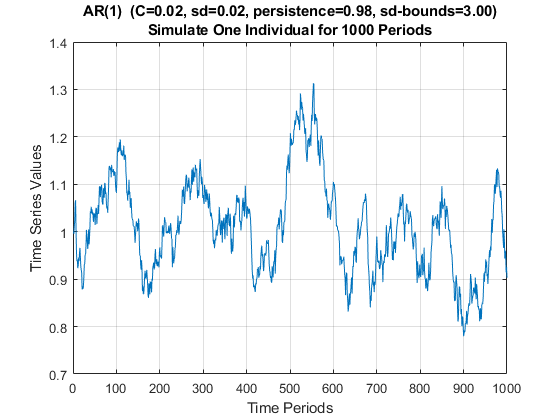
\includegraphics[width=5.20833in,height=\textheight]{img/fs_autoregressive_images/figure_0.png}

\hypertarget{income-process-for-india}{%
\subsubsection{Income Process for India}\label{income-process-for-india}}

In the Example below, we simulate an individual for 1000 periods. In the
example below, the parameters are from estiamting an AR(1) process for
log of income in India, see Udupa and Wang (2020). We can use the
\href{https://fanwangecon.github.io/MEconTools/MEconTools/doc/stats/htmlpdfm/fx_simu_stats.html}{ff\_simu\_stats}
function from \href{https://fanwangecon.github.io/MEconTools/}{MEconTools} to
look at the distributional information from this time series, we care
about income, so we will exponentiate the log of income we obtained.

Note that for the distributional results, GINI, share of income held by
different percentiles of households, is invariant to the choice of the
\(C\) constant term earlier. Try changing that number, the distributional
statistics that we obtain below will be the same. Also note that the
exponential of the mean of the log of income is not equal to the mean of
income.

\begin{verbatim}
% Number of Time Periods
it_T = 1000;
% Mean and SD of the Shock Process
fl_constant = 3.024467;
fl_normal_sd = 0.45;
% Persistence
fl_persistence = 0.7468;
% Bounds on Shocks
fl_shk_bnds = 5;
% Initialize with exo fed point or not, if false initialize at Random Point
% from the stationary distribution
bl_init = true;
fl_init = fl_constant/(1 - fl_persistence);
% Generate a normal shock vector (the first draw will be ignored)
it_draws = it_T;
rng(789);
ar_fl_shocks = normrnd(0, fl_normal_sd, 1, it_draws);
% out of bounds indicators
fl_shk_bds_lower = 0 - fl_normal_sd*fl_shk_bnds;
fl_shk_bds_upper = 0 + fl_normal_sd*fl_shk_bnds;
ar_bl_outofbounds = (ar_fl_shocks <= fl_shk_bds_lower | ar_fl_shocks >= fl_shk_bds_upper);
ar_fl_shocks(ar_fl_shocks <= fl_shk_bds_lower) = fl_shk_bds_lower;
ar_fl_shocks(ar_fl_shocks >= fl_shk_bds_upper) = fl_shk_bds_upper;
% Initialize Output Array
ar_fl_time_series = zeros(size(ar_fl_shocks));
% Loop over time
for it_t=1:1:length(ar_fl_shocks)
    if (it_t == 1)
        % initialize using the ean of the process
        ar_fl_time_series(1) = fl_constant/(1 - fl_persistence);
        if (bl_init)
            ar_fl_time_series(1) = fl_init;            
        end
    else
        fl_ts_t = fl_constant + ar_fl_time_series(it_t-1)*fl_persistence + ar_fl_shocks(it_t);
        ar_fl_time_series(it_t) = fl_ts_t;
    end
end
ar_series = (ar_fl_time_series);
fl_mean = mean(ar_series);
fl_std = std(ar_series);
figure();
% x-axis
ar_it_time = 1:1:length(ar_fl_shocks);
% plot
plot(ar_it_time, (ar_fl_time_series));
% Generate Title
ar_fl_params_values = [fl_constant, fl_normal_sd, fl_persistence, fl_shk_bnds];
ar_st_parms_names = ["C", "sd", "persistence", "sd-bounds"];
st_rounding = '.2f';
st_title_main = "AR(1) Log of Income in India";
ar_st_params = strcat(ar_st_parms_names, compose(strcat("=%", st_rounding), ar_fl_params_values));
st_param_pasted = strjoin(ar_st_params, ', ');
st_title_wth_params = strcat(st_title_main, ' (', st_param_pasted, ')');
title({st_title_wth_params, 'Simulate One Individual for 1000 Periods'});
% X and Y labels
ylabel({'Log of Income (India)'});
xlabel('Time Periods');
grid on;
\end{verbatim}

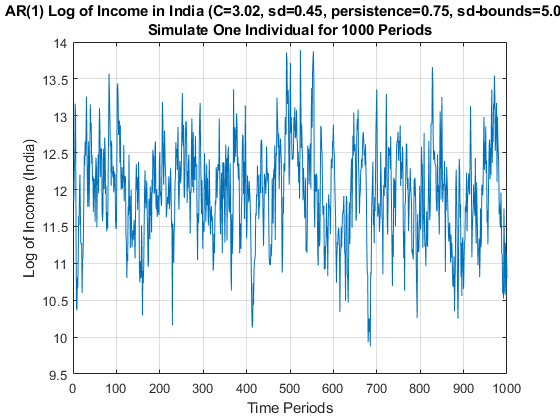
\includegraphics[width=5.20833in,height=\textheight]{img/fs_autoregressive_images/figure_1.png}

\begin{verbatim}
% Set Parameters
mp_cl_mt_xyz_of_s = containers.Map('KeyType','char', 'ValueType','any');
mp_cl_mt_xyz_of_s('log_income') = {(ar_series), zeros(1)};
mp_cl_mt_xyz_of_s('income') = {exp(ar_series), zeros(1)};
mp_cl_mt_xyz_of_s('ar_st_y_name') = ["log_income", "income"];
% Mass
rng(123);
mt_f_of_s = zeros(size(ar_series)) + 1/numel(ar_series);
mt_f_of_s = mt_f_of_s/sum(mt_f_of_s, 'all');
mp_cl_mt_xyz_of_s_out = ff_simu_stats(mt_f_of_s, mp_cl_mt_xyz_of_s);

xxx tb_outcomes: all stats xxx
    OriginalVariableNames    log_income      income  
    _____________________    __________    __________

    {'mean'             }       11.959      1.946e+05
    {'unweighted_sum'   }        11959      1.946e+08
    {'sd'               }      0.67236     1.4024e+05
    {'coefofvar'        }     0.056222        0.72064
    {'gini'             }     0.031635        0.35645
    {'min'              }       9.8742          19423
    {'max'              }       13.893      1.081e+06
    {'pYis0'            }            0              0
    {'pYls0'            }            0              0
    {'pYgr0'            }            1              1
    {'pYisMINY'         }        0.001          0.001
    {'pYisMAXY'         }        0.001          0.001
    {'p1'               }       10.258          28498
    {'p10'              }       11.087          65316
    {'p25'              }       11.518     1.0049e+05
    {'p50'              }       11.983        1.6e+05
    {'p75'              }        12.42     2.4771e+05
    {'p90'              }       12.761     3.4829e+05
    {'p99'              }       13.479      7.141e+05
    {'fl_cov_log_income'}      0.45207          84333
    {'fl_cor_log_income'}            1        0.89439
    {'fl_cov_income'    }        84333     1.9667e+10
    {'fl_cor_income'    }      0.89439              1
    {'fracByP1'         }    0.0093239      0.0014385
    {'fracByP10'        }     0.089816       0.024687
    {'fracByP25'        }       0.2317       0.088239
    {'fracByP50'        }      0.47761        0.25477
    {'fracByP75'        }      0.73265        0.51224
    {'fracByP90'        }      0.89045        0.73747
    {'fracByP99'        }      0.98852        0.95275
\end{verbatim}

\hypertarget{matlab-moving-average-of-time-series}{%
\subsection{Matlab Moving Average of Time-series}\label{matlab-moving-average-of-time-series}}

\begin{quote}
Go back to \href{http://fanwangecon.github.io/}{fan}'s \href{https://fanwangecon.github.io/MEconTools/}{MEconTools} Package, \href{https://fanwangecon.github.io/M4Econ/}{Matlab Code Examples} Repository (\href{https://fanwangecon.github.io/M4Econ/bookdown}{bookdown site}), or \href{https://fanwangecon.github.io/Math4Econ/}{Math for Econ with Matlab} Repository (\href{https://fanwangecon.github.io/Math4Econ/bookdown}{bookdown site}).
\end{quote}

\hypertarget{weighted-average-of-neighbors}{%
\subsubsection{Weighted Average of Neighbors}\label{weighted-average-of-neighbors}}

Not actually a time-series moving average. There is a vector of a
parameter value, this parameter is not been estimated, we estimate all
other parameters while varying this one parameter. At different values
of this parameter, there is a vector of estimates. We have estimated a
model along a equi-distance grid of this exogenous parameter. Now for
each of the estimated parameter, calculate a "moving-average" based on
averaging across estimated neighbor values of this parameter, where
neighbor distance is defined by the fixed exogenous parameter. Why do
this? This can be considered a "smoother" tool, but more importantly,
use the moving averages as new initial parameter guesses for a new round
of estimation at each of the exogenous parameter's values. For different
starting seeds, use different moving windows.

First, select out all estimates:

\begin{verbatim}
% Load in file
srn_excel_exa = 'C:\Users\fan\M4Econ\table\_exa\excel_exa.xlsx';
tb_estimates = readtable(srn_excel_exa);
% columns to select
ar_st_colnames = tb_estimates.Properties.VariableNames;
ar_st_colnames_sel = ["mean_h_sd", ar_st_colnames(endsWith(ar_st_colnames, '_esti'))];
% Select all estimates columns and the exogenous parameter column
mt_estimates_sel = tb_estimates{:, ar_st_colnames_sel};
% sort by the first column
mt_estimates_sel = sortrows(mt_estimates_sel, 1);
disp(mt_estimates_sel(1:10,:));

    0.0500   -3.4978   -2.6181   -2.7631   -0.9659   -0.4155   -3.1664   -4.4143
    0.1000   -3.5013   -2.6949   -2.8498   -0.9718   -0.4155   -3.1579   -4.4355
    0.1500   -3.4849   -2.8976   -3.0884   -0.9737   -0.4155   -3.1566   -4.4783
    0.2000   -3.4633   -2.7626   -2.9237   -0.9746   -0.4155   -3.1552   -4.5471
    0.2500   -3.3769   -1.4130   -1.4498   -0.9752   -0.4155   -3.1545   -4.7172
    0.3000   -3.3928   -2.7294   -2.8764   -0.9737   -0.4155   -3.1544   -4.7274
    0.3500   -3.3356   -2.5737   -2.6928   -0.9711   -0.4155   -3.1550   -4.8517
    0.4000   -3.1298   -1.7669   -1.8096   -0.9509   -0.4155   -3.1538   -5.8944
    0.4500   -3.1357   -2.2754   -2.3482   -0.9509   -0.4155   -3.1537   -6.0055
    0.5000   -3.1579   -2.6960   -2.8119   -0.9513   -0.4155   -3.1553   -6.0710

% show size
disp(size(mt_estimates_sel));

    82     8
\end{verbatim}

Second, calculate moving aveage with
\href{https://www.mathworks.com/help/matlab/ref/movmean.html\#bu6jxup}{movmean},
take the mean of up to 33 surrounding values, 66 and 99. Note that there
is only 82 elements of the array. But the movmean function's window
parameter will divide the window left and right.

\begin{verbatim}
mt_estimates_mov33 = movmean(mt_estimates_sel, 33);
mt_estimates_mov66 = movmean(mt_estimates_sel, 66);
mt_estimates_movflat = movmean(mt_estimates_sel, size(mt_estimates_sel,1)*2);
\end{verbatim}

Visualize using the
\href{https://fanwangecon.github.io/MEconTools/MEconTools/doc/graph/htmlpdfm/fx_graph_grid.html}{ff\_graph\_grid}
function from \href{https://fanwangecon.github.io/MEconTools/}{MEconTools}
moving average for one parameter, with different windows. Note that with
a moving window of 82*2, the moving average becomes flat, because there
are 82 elements of the underlying "time-series", so the window needs
to be 82*2 for the moving average to be fully flat.

\begin{verbatim}
% Generate some Data
ar_row_grid = ["actual", "moving avg widow=33","mov window=66","mov window=82*2"];
ar_exo_param_grid = mt_estimates_sel(:, 1);
it_col = 4;
mt_mov_value = [mt_estimates_sel(:,it_col), ...
    mt_estimates_mov33(:,it_col), ...
    mt_estimates_mov66(:,it_col), ...
    mt_estimates_movflat(:,it_col)]'; 
% container map settings
mp_support_graph = containers.Map('KeyType', 'char', 'ValueType', 'any');
mp_support_graph('cl_st_graph_title') = {'Moving Average with Widening Sliding Windows'};
mp_support_graph('cl_st_ytitle') = {'Parameter Estimates Moving Average'};
mp_support_graph('cl_st_xtitle') = {'Exogenous Parameter (not estimated)'};
mp_support_graph('st_legend_loc') = 'best';
mp_support_graph('bl_graph_logy') = false;
mp_support_graph('it_legend_select') = 4; % how many shock legends to show
mp_support_graph('st_rounding') = '6.2f'; % format shock legend
mp_support_graph('cl_scatter_shapes') = {'s', 'o', '*', 'x'};
mp_support_graph('cl_colors') = 'lines';
% Call function
ff_graph_grid(mt_mov_value, ar_row_grid, ar_exo_param_grid, mp_support_graph);
\end{verbatim}

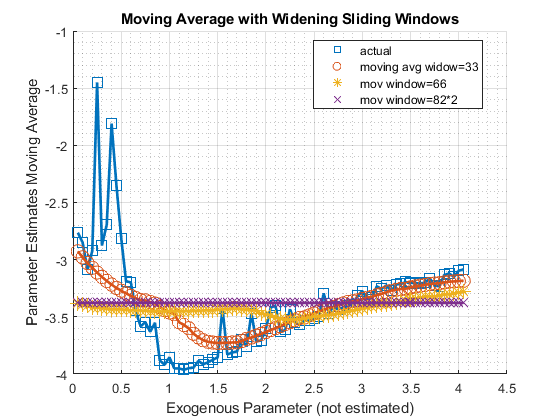
\includegraphics[width=5.20833in,height=\textheight]{img/fs_movingaverage_images/figure_0.png}

\hypertarget{cross-sectional-data}{%
\section{Cross-sectional Data}\label{cross-sectional-data}}

\hypertarget{matlab-mincer-wage-earnings-equation-with-experience-education-and-gamma-shocks}{%
\subsection{Matlab Mincer Wage Earnings Equation with Experience, Education and Gamma Shocks}\label{matlab-mincer-wage-earnings-equation-with-experience-education-and-gamma-shocks}}

\begin{quote}
Go back to \href{http://fanwangecon.github.io/}{fan}'s \href{https://fanwangecon.github.io/MEconTools/}{MEconTools} Package, \href{https://fanwangecon.github.io/M4Econ/}{Matlab Code Examples} Repository (\href{https://fanwangecon.github.io/M4Econ/bookdown}{bookdown site}), or \href{https://fanwangecon.github.io/Math4Econ/}{Math for Econ with Matlab} Repository (\href{https://fanwangecon.github.io/Math4Econ/bookdown}{bookdown site}).
\end{quote}

\hypertarget{define-a-wage-equation-with-partial-income-for-part-time-workss-1}{%
\subsubsection{Define a Wage Equation with Partial Income for Part-time Workss}\label{define-a-wage-equation-with-partial-income-for-part-time-workss-1}}

Individuals might work part or full time. Define a mincer wage equation
that is a function of experienc, education and other individual
characteristics. This is partly based on the wage equation from \href{https://www.sciencedirect.com/science/article/abs/pii/S1094202517300029}{Hai and
Heckman
(2017)}. \citep{HaiHeckman2017}

First define parameters.

\begin{verbatim}
% cognitive and non-cognitive latent types
theta_cogntv = 0.1;
theta_noncog = 0.1;
% parameters mapping latent types to wage
COEF_alpha_cog_wage_hsh = 0.0529;
COEF_alpha_cog_wage_clg = 0.0529;
COEF_alpha_cog_wage_grd = 0.1433;
COEF_alpha_ncg_wage_hsh = 0.0275;
COEF_alpha_ncg_wage_clg = 0.0512;
COEF_alpha_ncg_wage_grd = 0.0892;
% Experience
COEF_beta_psi_0 = 1.8884;
COEF_beta_psi_k = 0.0767;
COEF_beta_psi_kk = -0.2683;
% Education
COEF_beta_psi_e0 = 0.0465;
COEF_beta_w_e_1 = 0.1432;
COEF_beta_w_e_2 = 0.1435;
COEF_beta_w_e_3 = 0.2806;
% for part time
COEF_beta_w_part_0 = -0.0082;
COEF_beta_w_part_1 = -0.4863;
\end{verbatim}

Second define the log wage equation. This wage equation is a function of
the parameters defined above, and also Education (ED), experience (EX)
and the wage shcok (EPS\_w).

\begin{verbatim}
% Log of wage
f_log_psi = @(ED, EX, EPS_w) ...
    ((COEF_alpha_cog_wage_hsh.*theta_cogntv + COEF_alpha_ncg_wage_hsh.*theta_noncog).*(ED < 12) ...
    + (COEF_alpha_cog_wage_clg.*theta_cogntv + COEF_alpha_ncg_wage_clg.*theta_noncog).*(ED >= 12).*(ED < 16) ...
    + (COEF_alpha_cog_wage_grd.*theta_cogntv + COEF_alpha_ncg_wage_grd.*theta_noncog).*(ED >= 16) ...
    + COEF_beta_psi_0 ...
    + COEF_beta_psi_k.*EX ...
    + COEF_beta_psi_kk.*(EX.^2/100) ...
    + COEF_beta_psi_e0.*(ED - 12) ...
    + COEF_beta_w_e_1.*(ED == 12) ...
    + COEF_beta_w_e_2.*(ED > 12).*(ED < 16) ...
    + COEF_beta_w_e_3.*(ED >= 16) ...
    + EPS_w);
\end{verbatim}

Third, define wage, which might differ depending on work status as well
as schooling status. D\_e is schooling or not, which can take values of 0
or 1. D\_k is work status, which can take values or 0, 0.5 (part-time
work) and 1 (full-time work).

\begin{verbatim}
% Per hour wage considering part time, part time wage differ if also schooling
f_hr_wage = @(D_e, D_k, ED, EX, EPS_w) ...
    exp(f_log_psi(ED, EX, EPS_w)).*exp((D_k==0.5).*(COEF_beta_w_part_0 + COEF_beta_w_part_1.*D_e));
% Total wage
f_wage = @(D_e, D_k, ED, EX, EPS_w) ...
    f_hr_wage(D_e, D_k, ED, EX, EPS_w).*(2080.*(D_k == 1) + 1040.*(D_k == 0.5) + 0.*(D_k == 0));
\end{verbatim}

Fourth, test the wage equation by calling it with different work and
schooling choices, along with different education, experience, and shock
levels.

\begin{verbatim}
% no experience, education, not school, not work
disp(['f_wage(0,0,0,0,0)=' num2str(f_wage(0,0,0,0,0))]);

f_wage(0,0,0,0,0)=0

% no experience, education, part-time
disp(['f_wage(0,0.5,0,0,0)=' num2str(f_wage(0,0.5,0,0,0))]);

f_wage(0,0.5,0,0,0)=3933.229

% no experience, education, full-time
disp(['f_wage(0,1,0,0,0)=' num2str(f_wage(0,1,0,0,0))]);

f_wage(0,1,0,0,0)=7931.2281
\end{verbatim}

With the anonymous function defined, we can supply a vector of education
values (as a column), and a vector of experience levles (as a row), and
generate a matrix of wages for full-time workers, simulated at one
particular shock level. Graph using
\href{https://fanwangecon.github.io/MEconTools/MEconTools/doc/graph/htmlpdfm/fx_graph_grid.html}{FF\_GRAPH\_GRID}
from \href{https://fanwangecon.github.io/MEconTools/}{MEconTools}.

The graph shows that higher education corresponds to higher wages, there
are different levels by education tiers, and there is a quadratic
structure to experience

\begin{verbatim}
% 1 to 16 years of educations
ar_edu = 1:1:20;
% 1 to 20 years of experiences
ar_exp = 1:1:20;
% broadcast evaluate
mt_wages = f_wage(0,1,ar_edu',ar_exp,0);
% graph using MEconTools
mp_support_graph = containers.Map('KeyType', 'char', 'ValueType', 'any');
mp_support_graph('cl_st_graph_title') = {'wages(edu, exp, shk=0), exp=x, education=color'};
mp_support_graph('cl_st_ytitle') = {'wages(edu,exp)'};
mp_support_graph('cl_st_xtitle') = {'experience levels'};
mp_support_graph('bl_graph_logy') = false; % do not log
mp_support_graph('st_rowvar_name') = 'edu=';
mp_support_graph('it_legend_select') = 10; % how many shock legends to show
mp_support_graph('st_rounding') = '3.0f'; % format shock legend
mp_support_graph('cl_colors') = 'copper'; % any predefined matlab colormap
% Call function
ff_graph_grid(mt_wages, ar_edu, ar_exp, mp_support_graph);
\end{verbatim}

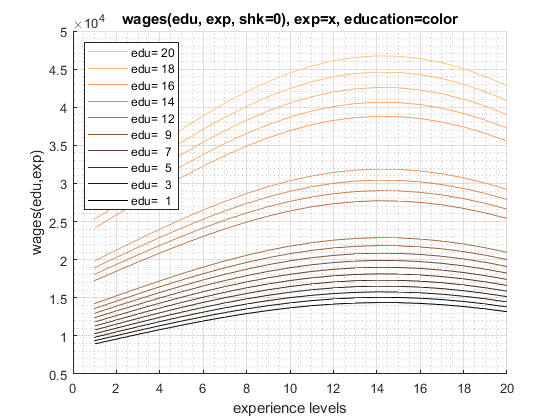
\includegraphics[width=5.20833in,height=\textheight]{img/fs_wage_equation_images/figure_0.png}

Draw the shock term from gamma distribution, distribution of wages at a
particular experience and education combination with many shocks.

\begin{verbatim}
% Gamma distribution parameters from Hai and Heckman
% E(epsilon) = a*b, var(epsion) = a*b^2.
a0 = 15.3558; % shape
b0 = 0.1388; % scale
% use gamrnd
it_draws = 10000;
ar_gamma_draws = gamrnd(a0, b0, [it_draws, 1]);
% Evaluate with 12 years of education and 10 years of experience with
% different shocks
ar_wages_e16_x10 = f_wage(0,1,16,10,ar_gamma_draws);
ar_wages_e12_x5 = f_wage(0,1,12,5,ar_gamma_draws);
\end{verbatim}

Draw a histogram of the wage distribution. \href{https://www.mathworks.com/help/matlab/ref/matlab.graphics.chart.primitive.histogram.html}{Multiple histograms in
matlab}.

\begin{verbatim}
figure();
h1 = histogram(log(ar_wages_e16_x10), 20);
hold on;
h2 = histogram(log(ar_wages_e12_x5), 20);
grid on;
h1.Normalization = 'probability';
h2.Normalization = 'probability';
% Put up legend.
legend1 = sprintf('Log wage dist edu=16 and exp=10');
legend2 = sprintf('Log wage dist edu=12 and exp=5');
legend({legend1, legend2});
\end{verbatim}

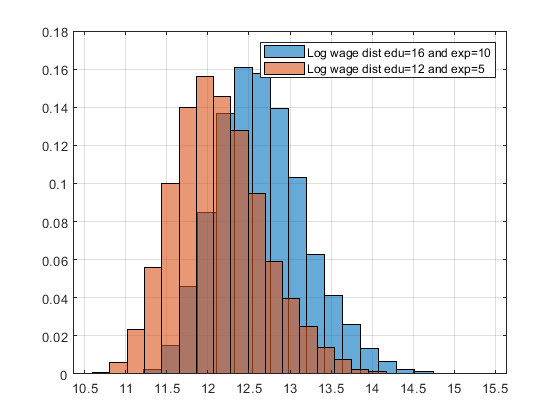
\includegraphics[width=5.20833in,height=\textheight]{img/fs_wage_equation_images/figure_1.png}

Generate distributional statistics using
\href{https://fanwangecon.github.io/MEconTools/MEconTools/doc/stats/htmlpdfm/fx_simu_stats.html}{FF\_SIMU\_STATS}
from \href{https://fanwangecon.github.io/MEconTools/}{MEconTools}. Given that
the shocks are the same, the distributional statistics in terms of gini,
and shares of wages held by different percentiles are the same. However,

\begin{verbatim}
% Set Parameters
mp_cl_mt_xyz_of_s = containers.Map('KeyType','char', 'ValueType','any');
mp_cl_mt_xyz_of_s('cl_wages_e16_x10') = {ar_wages_e16_x10, zeros(1)};
mp_cl_mt_xyz_of_s('cl_ar_wages_e12_x5') = {ar_wages_e12_x5, zeros(1)};
mp_cl_mt_xyz_of_s('ar_st_y_name') = ["cl_wages_e16_x10", "cl_ar_wages_e12_x5"];
% Mass
rng(123);
mt_f_of_s = 1/it_draws + zeros(size(ar_wages_e16_x10));
% Call Function
mp_cl_mt_xyz_of_s_out = ff_simu_stats(mt_f_of_s, mp_cl_mt_xyz_of_s);

xxx tb_outcomes: all stats xxx
        OriginalVariableNames        cl_wages_e16_x10    cl_ar_wages_e12_x5
    _____________________________    ________________    __________________

    {'mean'                     }       3.7009e+05           2.2035e+05
    {'unweighted_sum'           }       3.7009e+09           2.2035e+09
    {'sd'                       }       2.5548e+05           1.5212e+05
    {'coefofvar'                }          0.69034              0.69034
    {'gini'                     }          0.31929              0.31929
    {'min'                      }            72823                43359
    {'max'                      }       4.1108e+06           2.4476e+06
    {'pYis0'                    }                0                    0
    {'pYls0'                    }                0                    0
    {'pYgr0'                    }                1                    1
    {'pYisMINY'                 }           0.0001               0.0001
    {'pYisMAXY'                 }           0.0001               0.0001
    {'p1'                       }       1.0651e+05                63414
    {'p10'                      }       1.6176e+05                96313
    {'p25'                      }       2.1211e+05           1.2629e+05
    {'p50'                      }       3.0077e+05           1.7908e+05
    {'p75'                      }       4.4013e+05           2.6205e+05
    {'p90'                      }       6.5011e+05           3.8708e+05
    {'p99'                      }       1.3542e+06           8.0632e+05
    {'fl_cov_cl_wages_e16_x10'  }       6.5273e+10           3.8864e+10
    {'fl_cor_cl_wages_e16_x10'  }                1                    1
    {'fl_cov_cl_ar_wages_e12_x5'}       3.8864e+10            2.314e+10
    {'fl_cor_cl_ar_wages_e12_x5'}                1                    1
    {'fracByP1'                 }         0.002641             0.002641
    {'fracByP10'                }         0.036428             0.036428
    {'fracByP25'                }          0.11277              0.11277
    {'fracByP50'                }          0.28486              0.28486
    {'fracByP75'                }           0.5298               0.5298
    {'fracByP90'                }          0.74277              0.74277
    {'fracByP99'                }          0.95264              0.95264
\end{verbatim}

\hypertarget{simulation}{%
\chapter{Simulation}\label{simulation}}

\hypertarget{normal-distribution}{%
\section{Normal Distribution}\label{normal-distribution}}

\hypertarget{compute-cdf-for-normal-and-bivariate-normal-distributions}{%
\subsection{Compute CDF for Normal and Bivariate Normal Distributions}\label{compute-cdf-for-normal-and-bivariate-normal-distributions}}

\begin{quote}
Go back to \href{http://fanwangecon.github.io/}{fan}'s \href{https://fanwangecon.github.io/MEconTools/}{MEconTools} Package, \href{https://fanwangecon.github.io/M4Econ/}{Matlab Code Examples} Repository (\href{https://fanwangecon.github.io/M4Econ/bookdown}{bookdown site}), or \href{https://fanwangecon.github.io/Math4Econ/}{Math for Econ with Matlab} Repository (\href{https://fanwangecon.github.io/Math4Econ/bookdown}{bookdown site}).
\end{quote}

CDF for normal random variable through simulation and with NORMCDF
function. CDF for bivariate normal random variables through simulation
and with NORMCDF function.

\begin{itemize}
\item
  \href{https://fanwangecon.github.io/M4Econ/simulation/normal/htmlpdfm/fs_cholesky_decomposition.html}{fs\_cholesky\_decomposition}
\item
  \href{https://fanwangecon.github.io/M4Econ/simulation/normal/htmlpdfm/fs_cholesky_decomposition_d5.html}{fs\_cholesky\_decomposition\_d5}
\item
  \href{https://fanwangecon.github.io/M4Econ/simulation/normal/htmlpdfm/fs_bivariate_normal.html}{fs\_bivariate\_normal}
\end{itemize}

\hypertarget{simulate-normal-distribution-probability-with-uniform-draws}{%
\subsubsection{Simulate Normal Distribution Probability with Uniform Draws}\label{simulate-normal-distribution-probability-with-uniform-draws}}

Mean score is 0, standard deviation is 1, we want to know what is the
chance that children score less than -2, -1, 0, 1, and 2 respectively.
We have a solution to the normal CDF cumulative distribution problem, it
is:

\begin{verbatim}
mu = 0;
sigma = 1;
ar_x = [-2,-1,0,1,2];
for x=ar_x
    cdf_x = normcdf(x, mu, sigma);
    disp([strjoin(...
        ["CDF with normcdf", ...
        ['x=' num2str(x)] ...
        ['cdf_x=' num2str(cdf_x)] ...
        ], ";")]);
end

CDF with normcdf;x=-2;cdf_x=0.02275
CDF with normcdf;x=-1;cdf_x=0.15866
CDF with normcdf;x=0;cdf_x=0.5
CDF with normcdf;x=1;cdf_x=0.84134
CDF with normcdf;x=2;cdf_x=0.97725
\end{verbatim}

We can also approximate the probabilities above, by drawing many points
from a unifom:

\begin{enumerate}
\def\labelenumi{\arabic{enumi}.}
\item
  Draw from uniform distribution 0 to 1, N times.
\item
  Invert these using invnorm. This means our uniform draws are now
  effectively drawn from the normal distribution.
\item
  Check if each draw inverted is below the x threshold or above, count
  fractions.
\end{enumerate}

We should get very similar results as in the example above (especially
if N is large)

\begin{verbatim}
% set seed
rng(123);
% generate random numbers
N = 10000;
ar_unif_draws = rand(1,N);
% invert
ar_normal_draws = norminv(ar_unif_draws);
% loop over different x values
for x=ar_x
    % index if draws below x
    ar_it_idx_below_x = (ar_normal_draws < x);
    fl_frac_below_x = (sum(ar_it_idx_below_x))/N;
    disp([strjoin(...
        ["CDF with normcdf", ...
        ['x=' num2str(x)] ...
        ['fl_frac_below_x=' num2str(fl_frac_below_x)] ...
        ], ";")]);
end

CDF with normcdf;x=-2;fl_frac_below_x=0.023
CDF with normcdf;x=-1;fl_frac_below_x=0.1612
CDF with normcdf;x=0;fl_frac_below_x=0.4965
CDF with normcdf;x=1;fl_frac_below_x=0.847
CDF with normcdf;x=2;fl_frac_below_x=0.9789
\end{verbatim}

\hypertarget{simulate-bivariate-normal-distribution-probability-with-uniform-draws}{%
\subsubsection{Simulate Bivariate-Normal Distribution Probability with Uniform Draws}\label{simulate-bivariate-normal-distribution-probability-with-uniform-draws}}

There are two tests now, a math test and an English test. Student test
scores are correlated with correlation 0.5 from the two tests, mean and
standard deviations are 0 and 1 for both tests. What is the chance that
a student scores below -2 and -2 for both, below -2 and 0 for math and
English, below 2 and 1 for math and English, etc?

\begin{verbatim}
% timer
tm_start_mvncdf = tic;
% mean, and varcov
ar_mu = [0,0];
mt_varcov = [1,0.5;0.5,1];
ar_x = linspace(-3,3,101);
% initialize storage
mt_prob_math_eng = zeros([length(ar_x), length(ar_x)]);
% loop over math and english score thresholds
it_math = 0;
for math=ar_x
    it_math = it_math + 1;
    it_eng = 0;
    for eng=ar_x
        it_eng = it_eng + 1;
        % points below which to compute probability 
        ar_scores = [math, eng];
        % volumn of a mountain to the southwest of north-south and east-west cuts
        cdf_x = mvncdf(ar_scores, ar_mu, mt_varcov);
        mt_prob_math_eng(it_math, it_eng) = cdf_x;
    end
end
% end timer
tm_end_mvncdf = toc(tm_start_mvncdf);
st_complete = strjoin(...
    ["MVNCDF Completed CDF computes", ...
     ['number of points=' num2str(numel(mt_prob_math_eng))] ...
     ['time=' num2str(tm_end_mvncdf)] ...
    ], ";");
disp(st_complete);

MVNCDF Completed CDF computes;number of points=10201;time=1.1957

% show results
tb_prob_math_eng = array2table(round(mt_prob_math_eng, 4));
cl_col_names_a = strcat('english <=', string(ar_x'));
cl_row_names_a = strcat('math <=', string(ar_x'));
tb_prob_math_eng.Properties.VariableNames = cl_col_names_a;
tb_prob_math_eng.Properties.RowNames = cl_row_names_a;
% subsetting function
% https://fanwangecon.github.io/M4Econ/amto/array/htmlpdfm/fs_slicing.html#19_Given_Array_of_size_M,_Select_N_somewhat_equi-distance_elements
f_subset = @(it_subset_n, it_ar_n) unique(round(((0:1:(it_subset_n-1))/(it_subset_n-1))*(it_ar_n-1)+1));
disp(tb_prob_math_eng(f_subset(7, length(ar_x)), f_subset(7, length(ar_x))));

                    english <=-3    english <=-1.98    english <=-1.02    english <=0    english <=1.02    english <=1.98    english <=3
                    ____________    _______________    _______________    ___________    ______________    ______________    ___________

    math <=-3          0.0001           0.0005              0.001           0.0013           0.0013            0.0013          0.0013   
    math <=-1.98       0.0005           0.0043             0.0136           0.0217           0.0237            0.0238          0.0239   
    math <=-1.02        0.001           0.0136             0.0598           0.1239           0.1505            0.1537          0.1539   
    math <=0           0.0013           0.0217             0.1239           0.3333           0.4701            0.4978             0.5   
    math <=1.02        0.0013           0.0237             0.1505           0.4701           0.7521            0.8359          0.8458   
    math <=1.98        0.0013           0.0238             0.1537           0.4978           0.8359            0.9566          0.9753   
    math <=3           0.0013           0.0239             0.1539              0.5           0.8458            0.9753          0.9974   
\end{verbatim}

We can also approximate the probabilities above, by drawing many points
from two iid uniforms, and translating them to correlated normal using
cholesky decomposition:

\begin{enumerate}
\def\labelenumi{\arabic{enumi}.}
\item
  Draw from two random uniform distribution 0 to 1, N times each
\item
  Invert these using invnorm for both iid vectors from unifom draws to
  normal draws
\item
  Choleskey decompose and multiplication
\end{enumerate}

This method below is faster than the method above when the number of
points where we have to evaluat probabilities is large.

Generate randomly drawn scores:

\begin{verbatim}
% timer
tm_start_chol = tic;
% Draws uniform and invert to standard normal draws
N = 10000;
rng(123);
ar_unif_draws = rand(1,N*2);
ar_normal_draws = norminv(ar_unif_draws);
ar_draws_eta_1 = ar_normal_draws(1:N);
ar_draws_eta_2 = ar_normal_draws((N+1):N*2);

% Choesley decompose the variance covariance matrix
mt_varcov_chol = chol(mt_varcov, 'lower');

% Generate correlated random normals
mt_scores_chol = ar_mu' + mt_varcov_chol*([ar_draws_eta_1; ar_draws_eta_2]);
ar_math_scores = mt_scores_chol(1,:)';
ar_eng_scores = mt_scores_chol(2,:)';
\end{verbatim}

Approximate probabilities from randomly drawn scores:

\begin{verbatim}
% initialize storage
mt_prob_math_eng_approx = zeros([length(ar_x), length(ar_x)]);
% loop over math and english score thresholds
it_math = 0;
for math=ar_x
    it_math = it_math + 1;
    it_eng = 0;
    for eng=ar_x
        it_eng = it_eng + 1;
        
        % points below which to compute probability 
        % index if draws below x
        ar_it_idx_below_x_math = (ar_math_scores < math);
        ar_it_idx_below_x_eng = (ar_eng_scores < eng);
        ar_it_idx_below_x_joint = ar_it_idx_below_x_math.*ar_it_idx_below_x_eng;
        fl_frac_below_x_approx = (sum(ar_it_idx_below_x_joint))/N;
        
        % volumn of a mountain to the southwest of north-south and east-west cuts
        mt_prob_math_eng_approx(it_math, it_eng) = fl_frac_below_x_approx;
    end
end
% end timer
tm_end_chol = toc(tm_start_chol);
st_complete = strjoin(...
    ["UNIF+CHOL Completed CDF computes", ...
     ['number of points=' num2str(numel(mt_prob_math_eng_approx))] ...
     ['time=' num2str(tm_end_chol)] ...
    ], ";");
disp(st_complete);

UNIF+CHOL Completed CDF computes;number of points=10201;time=0.28661

% show results
tb_prob_math_eng_approx = array2table(round(mt_prob_math_eng_approx, 4));
cl_col_names_a = strcat('english <=', string(ar_x'));
cl_row_names_a = strcat('math <=', string(ar_x'));
tb_prob_math_eng_approx.Properties.VariableNames = cl_col_names_a;
tb_prob_math_eng_approx.Properties.RowNames = cl_row_names_a;
disp(tb_prob_math_eng_approx(f_subset(7, length(ar_x)), f_subset(7, length(ar_x))));

                    english <=-3    english <=-1.98    english <=-1.02    english <=0    english <=1.02    english <=1.98    english <=3
                    ____________    _______________    _______________    ___________    ______________    ______________    ___________

    math <=-3          0.0001           0.0005              0.001           0.0016           0.0016            0.0016          0.0016   
    math <=-1.98       0.0003            0.004             0.0132           0.0218           0.0237            0.0239          0.0239   
    math <=-1.02       0.0008           0.0131              0.061           0.1272           0.1529             0.157          0.1571   
    math <=0           0.0009           0.0202             0.1236            0.334           0.4661            0.4946          0.4965   
    math <=1.02        0.0009           0.0215             0.1493           0.4724            0.754            0.8411          0.8511   
    math <=1.98        0.0009           0.0217             0.1526           0.4989           0.8344            0.9591           0.977   
    math <=3           0.0009           0.0217             0.1526           0.5007           0.8425            0.9768          0.9976   
\end{verbatim}

\hypertarget{cholesky-decomposition-correlated-bivariate-normal-from-iid-random-draws}{%
\subsection{Cholesky Decomposition Correlated Bivariate Normal from IID Random Draws}\label{cholesky-decomposition-correlated-bivariate-normal-from-iid-random-draws}}

\begin{quote}
Go back to \href{http://fanwangecon.github.io/}{fan}'s \href{https://fanwangecon.github.io/MEconTools/}{MEconTools} Package, \href{https://fanwangecon.github.io/M4Econ/}{Matlab Code Examples} Repository (\href{https://fanwangecon.github.io/M4Econ/bookdown}{bookdown site}), or \href{https://fanwangecon.github.io/Math4Econ/}{Math for Econ with Matlab} Repository (\href{https://fanwangecon.github.io/Math4Econ/bookdown}{bookdown site}).
\end{quote}

Draw two correlated normal shocks using the MVNRND function. Draw two
correlated normal shocks from uniform random variables using Cholesky
Decomposition.

\begin{itemize}
\item
  \href{https://fanwangecon.github.io/M4Econ/simulation/normal/htmlpdfm/fs_cholesky_decomposition.html}{fs\_cholesky\_decomposition}
\item
  \href{https://fanwangecon.github.io/M4Econ/simulation/normal/htmlpdfm/fs_cholesky_decomposition_d5.html}{fs\_cholesky\_decomposition\_d5}
\item
  \href{https://fanwangecon.github.io/M4Econ/simulation/normal/htmlpdfm/fs_bivariate_normal.html}{fs\_bivariate\_normal}
\end{itemize}

\hypertarget{positively-correlated-scores-mvnrnd}{%
\subsubsection{Positively Correlated Scores MVNRND}\label{positively-correlated-scores-mvnrnd}}

We have English and Math scores, and we draw from a bivariate normal
distribution, assuming the two scores are positively correlatd. These
are \(x_1\) and \(x_2\).

\begin{verbatim}
% mean, and varcov
ar_mu = [70,80];
mt_varcov = [8,5;5,5];
% Generate Scores
rng(123);
N = 10000;
mt_scores = mvnrnd(ar_mu, mt_varcov, N);
% graph
figure();
scatter(mt_scores(:,1), mt_scores(:,2));
ylabel('English Scores');
xlabel('Math Scores')
grid on;
\end{verbatim}

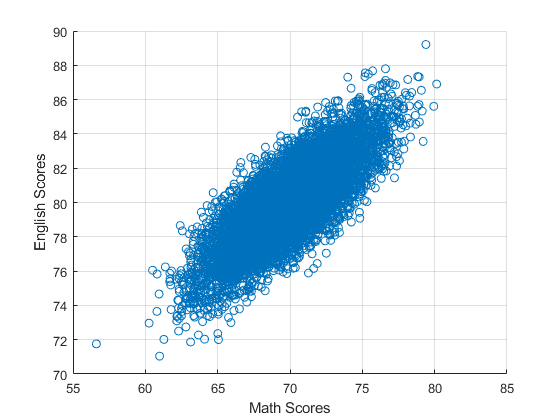
\includegraphics[width=5.20833in,height=\textheight]{img/fs_cholesky_decomposition_images/figure_0.png}

What are the covariance and correlation statistics?

\begin{verbatim}
disp([num2str(cov(mt_scores(:,1), mt_scores(:,2)))]);

8.0557      5.0738
5.0738      5.0638

disp([num2str(corrcoef(mt_scores(:,1), mt_scores(:,2)))]);

      1     0.79441
0.79441           1
\end{verbatim}

\hypertarget{bivariate-normal-from-uncorrelated-draws-via-cholesky-decomposition}{%
\subsubsection{Bivariate Normal from Uncorrelated Draws via Cholesky Decomposition}\label{bivariate-normal-from-uncorrelated-draws-via-cholesky-decomposition}}

We can get the same results as above, without having to explicitly draw
from a multivariate distribution by (For more details see \href{https://eml.berkeley.edu/~train/distant.html}{Train
(2009)}):

\begin{enumerate}
\def\labelenumi{\arabic{enumi}.}
\item
  Draw 2 uniform random iid vectors.
\item
  Convert to normal iid vectors.
\item
  Generate the test scores as a function of the two random variables,
  using Cholesky matrix.
\end{enumerate}

\underline{\textbf{\emph{First}}}, draw two uncorrelated normal random variables, with
mean 0, sd 1, \(\eta_1\) and \(\eta_2\).

\begin{verbatim}
% Draw Two Uncorrelated Normal Random Variables
% use the same N as above
rng(123);
% uniform draws, uncorrelated
ar_unif_draws = rand(1,N*2);
% normal draws, english and math are uncorreated
% ar_draws_eta_1 and ar_draws_eta_2 are uncorrelated by construction
ar_normal_draws = norminv(ar_unif_draws);
ar_draws_eta_1 = ar_normal_draws(1:N);
ar_draws_eta_2 = ar_normal_draws((N+1):N*2);
% graph
figure();
scatter(ar_draws_eta_1, ar_draws_eta_2);
ylabel('iid eta 1 draws');
xlabel('iid eta 2 draws')
grid on;
\end{verbatim}

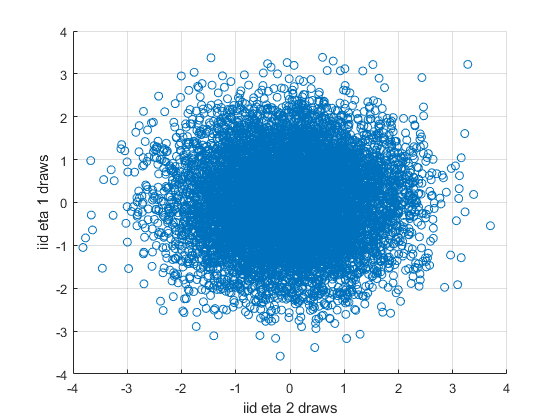
\includegraphics[width=5.20833in,height=\textheight]{img/fs_cholesky_decomposition_images/figure_1.png}

\begin{verbatim}
% Show Mean 1, cov = 0
disp([num2str(cov(ar_draws_eta_1, ar_draws_eta_2))]);

  0.99075   0.0056929
0.0056929     0.98517

disp([num2str(corrcoef(ar_draws_eta_1, ar_draws_eta_2))]);

        1   0.0057623
0.0057623           1
\end{verbatim}

\underline{\textbf{\emph{Second}}}, now using the variance-covariance we already have,
decompose it, we will have:

\begin{itemize}
\tightlist
\item
  \(\displaystyle \begin{array}{l} c_{aa} \,,\,\,0\\ c_{ab} \,,\,\,c_{bb} \end{array}\)
\end{itemize}

\begin{verbatim}
% Choesley decompose the variance covariance matrix
mt_varcov_chol = chol(mt_varcov, 'lower');
disp([num2str(mt_varcov_chol)]);

2.8284           0
1.7678      1.3693

% The cholesky decomposed matrix factorizes the original varcov matrix
disp([num2str(mt_varcov_chol*mt_varcov_chol')]);

8           5
5           5
\end{verbatim}

\underline{\textbf{\emph{Third}}}, We can get back to the original \(x_1\) and \(x_2\)
variables:

\begin{itemize}
\item
  \(\displaystyle x_1 =\mu_1 +c_{aa} *\eta_1\)
\item
  \(\displaystyle x_2 =\mu_2 +c_{ab} *\eta_1 +c_{bb} *\eta_2\)
\end{itemize}

\begin{verbatim}
% multiple the cholesky matrix by the eta draws
mt_scores_chol = ar_mu' + mt_varcov_chol*([ar_draws_eta_1; ar_draws_eta_2]);
mt_scores_chol = mt_scores_chol';
% graph
figure();
scatter(mt_scores_chol(:,1), mt_scores_chol(:,2));
ylabel('English Scores Chol from iid Draws = m1 + c\_aa*eta\_1');
xlabel('Math Scores Chol from iid Draws = m2 + c\_ab*eta\_1 + c\_bb*eta\_2')
grid on;
\end{verbatim}

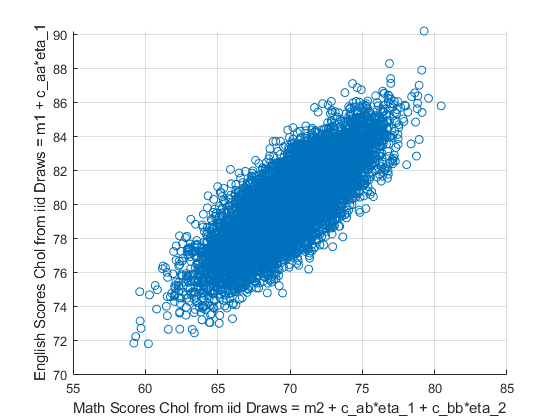
\includegraphics[width=5.20833in,height=\textheight]{img/fs_cholesky_decomposition_images/figure_2.png}

\begin{verbatim}
disp([num2str(cov(mt_scores_chol(:,1), mt_scores_chol(:,2)))]);

 7.926      4.9758
4.9758      4.9708

disp([num2str(corrcoef(mt_scores_chol(:,1), mt_scores_chol(:,2)))]);

      1     0.79272
0.79272           1
\end{verbatim}

\hypertarget{cholesky-decomposition-correlated-five-dimensional-multivariate-normal-shock}{%
\subsection{Cholesky Decomposition Correlated Five Dimensional Multivariate Normal Shock}\label{cholesky-decomposition-correlated-five-dimensional-multivariate-normal-shock}}

\begin{quote}
Go back to \href{http://fanwangecon.github.io/}{fan}'s \href{https://fanwangecon.github.io/MEconTools/}{MEconTools} Package, \href{https://fanwangecon.github.io/M4Econ/}{Matlab Code Examples} Repository (\href{https://fanwangecon.github.io/M4Econ/bookdown}{bookdown site}), or \href{https://fanwangecon.github.io/Math4Econ/}{Math for Econ with Matlab} Repository (\href{https://fanwangecon.github.io/Math4Econ/bookdown}{bookdown site}).
\end{quote}

Generate variance-covariance matrix from correlation and standard
deviation. Draw five correlated normal shocks using the MVNRND function.
Draw five correlated normal shocks from uniform random variables using
Cholesky Decomposition.

\begin{itemize}
\item
  \href{https://fanwangecon.github.io/M4Econ/simulation/normal/htmlpdfm/fs_cholesky_decomposition.html}{fs\_cholesky\_decomposition}
\item
  \href{https://fanwangecon.github.io/M4Econ/simulation/normal/htmlpdfm/fs_cholesky_decomposition_d5.html}{fs\_cholesky\_decomposition\_d5}
\item
  \href{https://fanwangecon.github.io/M4Econ/simulation/normal/htmlpdfm/fs_bivariate_normal.html}{fs\_bivariate\_normal}
\end{itemize}

\hypertarget{correlation-and-standard-deviations-to-variance-covariance-matrix}{%
\subsubsection{Correlation and Standard Deviations to Variance Covariance Matrix}\label{correlation-and-standard-deviations-to-variance-covariance-matrix}}

Given correlations and standard deviations, what is the variance and
covariance matrix? Assume mean 0. The first three variables are
correlated, the final two are iid.

First the ingredients:

\begin{verbatim}
% mean array
ar_mu = [0,0,0,0,0];
% standard deviations
ar_sd = [0.3301, 0.3329, 0.3308, 2312, 13394];
% correlations 
mt_cor = ...
    [1,0.1226,0.0182,0,0;...
     0.1226,1,0.4727,0,0;...
     0.0182,0.4727,1,0,0;...
     0,0,0,1,0;...
     0,0,0,0,1];
% show
disp(mt_cor);

    1.0000    0.1226    0.0182         0         0
    0.1226    1.0000    0.4727         0         0
    0.0182    0.4727    1.0000         0         0
         0         0         0    1.0000         0
         0         0         0         0    1.0000
\end{verbatim}

Second, we know that variance is the square of standard deviation. And
we know the formula for covariance, which is variance divided by two
standard deviations. So for the example here, we have:

\begin{verbatim}
% initialize
mt_varcov = zeros([5,5]);
% variance
mt_varcov(eye(5)==1) = ar_sd.^2;
% covariance
mt_varcov(1,2) = mt_cor(1,2)*ar_sd(1)*ar_sd(2);
mt_varcov(2,1) = mt_varcov(1,2);
mt_varcov(1,3) = mt_cor(1,3)*ar_sd(1)*ar_sd(3);
mt_varcov(3,1) = mt_varcov(1,3);
mt_varcov(2,3) = mt_cor(2,3)*ar_sd(2)*ar_sd(3);
mt_varcov(3,2) = mt_varcov(2,3);
% show
disp(mt_varcov(1:3,1:3));

    0.1090    0.0135    0.0020
    0.0135    0.1108    0.0521
    0.0020    0.0521    0.1094

disp(mt_varcov(4:5,4:5));

     5345344           0
           0   179399236
\end{verbatim}

\hypertarget{draw-five-correlated-shocks-using-mvnrnd}{%
\subsubsection{Draw Five Correlated Shocks Using MVNRND}\label{draw-five-correlated-shocks-using-mvnrnd}}

Generate N5 correlated shock structure

\begin{verbatim}
% Generate Scores
rng(123);
N = 50000;
mt_kw97_eps = mvnrnd(ar_mu, mt_varcov, N);
% graph
figure();
% subfigure 1
subplot(2,2,1);
scatter(mt_kw97_eps(:,1), mt_kw97_eps(:,2));
ylabel('White Collar Wage Shock');
xlabel('Blue Collar Wage Shock')
grid on;
% subfigure 2
subplot(2,2,2);
scatter(mt_kw97_eps(:,1), mt_kw97_eps(:,3));
ylabel('White Collar Wage Shock');
xlabel('Military Wage Shock')
grid on;
% subfigure 3
subplot(2,2,3);
scatter(mt_kw97_eps(:,3), mt_kw97_eps(:,2));
ylabel('Military Wage Shock');
xlabel('Blue Collar Wage Shock')
grid on;
% subfigure 4
subplot(2,2,4);
scatter(mt_kw97_eps(:,1), mt_kw97_eps(:,4));
ylabel('White Collar Wage Shock');
xlabel('School Shock')
grid on;
\end{verbatim}

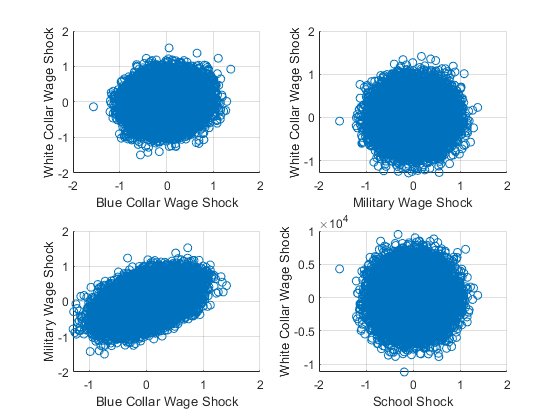
\includegraphics[width=5.20833in,height=\textheight]{img/fs_cholesky_decomposition_d5_images/figure_0.png}

What are the covariance and correlation statistics?

\begin{verbatim}
disp([num2str(round(corrcoef(mt_kw97_eps),3))]);

     1       0.119       0.016       0.002      -0.003
 0.119           1       0.468      -0.003       0.004
 0.016       0.468           1      -0.003       0.001
 0.002      -0.003      -0.003           1      -0.005
-0.003       0.004       0.001      -0.005           1

disp([num2str(round(corrcoef(mt_kw97_eps),2))]);

   1        0.12        0.02           0           0
0.12           1        0.47           0           0
0.02        0.47           1           0           0
   0           0           0           1       -0.01
   0           0           0       -0.01           1
\end{verbatim}

\hypertarget{draw-five-correlated-shocks-using-cholesky-decomposition}{%
\subsubsection{Draw Five Correlated Shocks Using Cholesky Decomposition}\label{draw-five-correlated-shocks-using-cholesky-decomposition}}

Following what we did for bivariate normal distribution, we can now do
the same for five different shocks at the same time (For more details
see \href{https://eml.berkeley.edu/~train/distant.html}{Train (2009)}):

\begin{enumerate}
\def\labelenumi{\arabic{enumi}.}
\item
  Draw 5 normal random variables that are uncorrelated
\item
  Generate 5 correlated shocks
\end{enumerate}

Draw the shocks

\begin{verbatim}
% Draws uniform and invert to standard normal draws
rng(123);
ar_unif_draws = rand(1,N*5);
ar_normal_draws = norminv(ar_unif_draws);
ar_draws_eta_1 = ar_normal_draws((N*0+1):N*1);
ar_draws_eta_2 = ar_normal_draws((N*1+1):N*2);
ar_draws_eta_3 = ar_normal_draws((N*2+1):N*3);
ar_draws_eta_4 = ar_normal_draws((N*3+1):N*4);
ar_draws_eta_5 = ar_normal_draws((N*4+1):N*5);

% Choesley decompose the variance covariance matrix
mt_varcov_chol = chol(mt_varcov, 'lower');

% Generate correlated random normals
mt_kp97_eps_chol = ar_mu' + mt_varcov_chol*([...
    ar_draws_eta_1; ar_draws_eta_2; ar_draws_eta_3; ar_draws_eta_4; ar_draws_eta_5]);
mt_kp97_eps_chol = mt_kp97_eps_chol';
\end{verbatim}

Graph:

\begin{verbatim}
% graph
figure();
% subfigure 1
subplot(2,2,1);
scatter(mt_kp97_eps_chol(:,1), mt_kp97_eps_chol(:,2));
ylabel('CHOL White Collar Wage Shock');
xlabel('CHOL Blue Collar Wage Shock')
grid on;
% subfigure 2
subplot(2,2,2);
scatter(mt_kp97_eps_chol(:,1), mt_kp97_eps_chol(:,3));
ylabel('CHOL White Collar Wage Shock');
xlabel('CHOL Military Wage Shock')
grid on;
% subfigure 3
subplot(2,2,3);
scatter(mt_kp97_eps_chol(:,3), mt_kp97_eps_chol(:,2));
ylabel('CHOL Military Wage Shock');
xlabel('CHOL Blue Collar Wage Shock')
grid on;
% subfigure 4
subplot(2,2,4);
scatter(mt_kp97_eps_chol(:,1), mt_kp97_eps_chol(:,4));
ylabel('CHOL White Collar Wage Shock');
xlabel('CHOL School Shock')
grid on;
\end{verbatim}

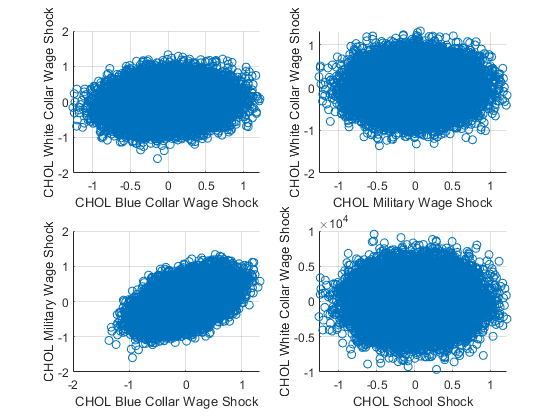
\includegraphics[width=5.20833in,height=\textheight]{img/fs_cholesky_decomposition_d5_images/figure_1.png}

What are the covariance and correlation statistics?

\begin{verbatim}
disp([num2str(round(corrcoef(mt_kp97_eps_chol),3))]);

     1       0.119       0.021       0.008      -0.003
 0.119           1       0.479       0.008      -0.003
 0.021       0.479           1       0.002           0
 0.008       0.008       0.002           1      -0.004
-0.003      -0.003           0      -0.004           1

disp([num2str(round(corrcoef(mt_kp97_eps_chol),2))]);

   1        0.12        0.02        0.01           0
0.12           1        0.48        0.01           0
0.02        0.48           1           0           0
0.01        0.01           0           1           0
   0           0           0           0           1
\end{verbatim}

\hypertarget{estimation}{%
\chapter{Estimation}\label{estimation}}

\hypertarget{linear-estimation}{%
\section{Linear Estimation}\label{linear-estimation}}

\hypertarget{linear-ols-estimation}{%
\subsection{Linear OLS Estimation}\label{linear-ols-estimation}}

\begin{quote}
Go back to \href{http://fanwangecon.github.io/}{fan}'s \href{https://fanwangecon.github.io/MEconTools/}{MEconTools} Package, \href{https://fanwangecon.github.io/M4Econ/}{Matlab Code Examples} Repository (\href{https://fanwangecon.github.io/M4Econ/bookdown}{bookdown site}), or \href{https://fanwangecon.github.io/Math4Econ/}{Math for Econ with Matlab} Repository (\href{https://fanwangecon.github.io/Math4Econ/bookdown}{bookdown site}).
\end{quote}

\hypertarget{estimation-without-an-intercept}{%
\subsubsection{Estimation without an Intercept}\label{estimation-without-an-intercept}}

Fit a line from the origin through two points, given Equations
\(Y=a\cdot X\), where we have two pairs of points for x and y.

\begin{verbatim}
rng(3);
[x1, x2] = deal(rand(),rand());
[y1, y2] = deal(rand(),rand());
ar_x = [x1,x2]';
ar_y = [y1,y2]';
\end{verbatim}

Fit a line through the two points, passing through the x-intercept.
Three formulas that provide the same answer.

\begin{verbatim}
% simple formula
fl_slope_basic = (1/(x1*x1 + x2*x2))*(x1*y1 + x2*y2);
% (X'X)^(-1)(X'Y)
fl_slope_matrix = inv(ar_x'*ar_x)*(ar_x'*ar_y);
% Use matlab function
tb_slope_fitlm = fitlm(ar_x, ar_y, 'Intercept',false);
fl_slope_fitlm = tb_slope_fitlm.Coefficients{1, 1};
\end{verbatim}

Visualize results.

\begin{verbatim}
figure();
hold on;
scatter([x1,x2], [y1,y2]);
xlim([0, 1]);
ylim([0, 1]);
refline(fl_slope_basic, 0);
grid on;
grid minor;
title('Best fit line through origin with two points');
\end{verbatim}

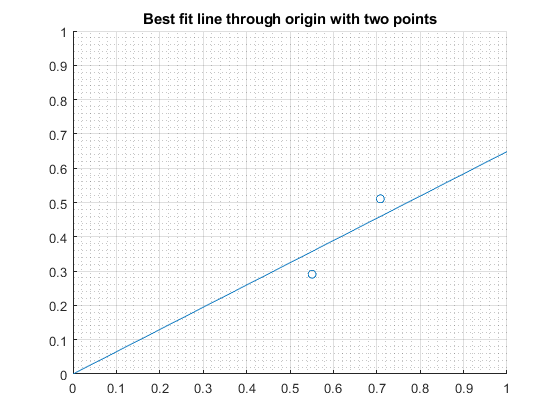
\includegraphics[width=5.20833in,height=\textheight]{img/fs_linear_ols_images/figure_0.png}

\hypertarget{nonlinear-estimation}{%
\section{Nonlinear Estimation}\label{nonlinear-estimation}}

\hypertarget{nonlinear-estimation-with-fminunc}{%
\subsection{Nonlinear Estimation with Fminunc}\label{nonlinear-estimation-with-fminunc}}

\begin{quote}
Go back to \href{http://fanwangecon.github.io/}{fan}'s \href{https://fanwangecon.github.io/MEconTools/}{MEconTools} Package, \href{https://fanwangecon.github.io/M4Econ/}{Matlab Code Examples} Repository (\href{https://fanwangecon.github.io/M4Econ/bookdown}{bookdown site}), or \href{https://fanwangecon.github.io/Math4Econ/}{Math for Econ with Matlab} Repository (\href{https://fanwangecon.github.io/Math4Econ/bookdown}{bookdown site}).
\end{quote}

\hypertarget{nonlinear-estimation-inputs-lhs-and-rhs}{%
\subsubsection{Nonlinear Estimation Inputs LHS and RHS}\label{nonlinear-estimation-inputs-lhs-and-rhs}}

Estimate this equation:
\(\omega_t =\left(\nu_0 +a_0 \right)+a_1 t-\log \left(1-\exp \left(a_0 +a_1 t\right)\right)+\nu_t\).
We have data from multiple \(t\), and want to estimate the \(a_0\), and
\(a_1\) coefficients mainly, but also \(\nu_0\) is good as well. This is an
estimation problem with 3 unknowns. \(t\) ranges from

\begin{verbatim}
% LHS outcome variable
ar_w = [-1.7349,-1.5559,-1.4334,-1.3080,-1.1791,-1.0462,-0.9085,-0.7652,-0.6150,-0.4564,-0.2874,-0.1052,0.0943];
% RHS t variable
ar_t = [0,3,5,7,9,11,13,15,16,19,21,23,25];
% actual parameters, estimation checks if gets actual parameters back
ar_a = [-1.8974, 0.0500];
\end{verbatim}

\hypertarget{prediction-and-mse-equations}{%
\subsubsection{Prediction and MSE Equations}\label{prediction-and-mse-equations}}

Objective function for prediction and mean-squared-error.

\begin{verbatim}
obj_ar_predictions = @(a) (v_0 + a(1) + a(2).*ar_t - log(1 - exp(a(1) + a(2).*ar_t)));
obj_fl_mse = @(a) mean((obj_ar_predictions(a) - ar_w).^2);
\end{verbatim}

Evaluate given ar\_a vectors.

\begin{verbatim}
ar_predict_at_actual = obj_ar_predictions(ar_a);
fl_mse_at_actual = obj_fl_mse(ar_a);
mt_compare = [ar_w', ar_predict_at_actual'];
tb_compare = array2table(mt_compare);
tb_compare.Properties.VariableNames = {'lhs-outcomes', 'evaluate-rhs-at-actual-parameters'};
disp(tb_compare);

    lhs-outcomes    evaluate-rhs-at-actual-parameters
    ____________    _________________________________

      -1.7349                    -1.7349             
      -1.5559                     -1.556             
      -1.4334                    -1.4335             
       -1.308                    -1.3081             
      -1.1791                    -1.1793             
      -1.0462                    -1.0464             
      -0.9085                   -0.90877             
      -0.7652                   -0.76546             
       -0.615                   -0.69133             
      -0.4564                   -0.45679             
      -0.2874                   -0.28786             
      -0.1052                   -0.10571             
       0.0943                   0.093688             
\end{verbatim}

\hypertarget{unconstrained-nonlinear-estimation}{%
\subsubsection{Unconstrained Nonlinear Estimation}\label{unconstrained-nonlinear-estimation}}

Estimation to minimize mean-squared-error.

\begin{verbatim}
% Estimation options
options = optimset('display','off');
% Starting values
ar_a_init = [-10, -10];
% Optimize
[ar_a_opti, fl_fval] = fminunc(obj_est, ar_a_init, options);
\end{verbatim}

Compare results.

\begin{verbatim}
mt_compare = [ar_a_opti', ar_a'];
tb_compare = array2table(mt_compare);
tb_compare.Properties.VariableNames = {'estimated-best-fit', 'actual-parameters'};
disp(tb_compare);

    estimated-best-fit    actual-parameters
    __________________    _________________

          -1.8939              -1.8974     
         0.050037                 0.05     
\end{verbatim}

\hypertarget{graphs}{%
\chapter{Graphs}\label{graphs}}

\hypertarget{figure-components}{%
\section{Figure Components}\label{figure-components}}

\hypertarget{matlab-graph-safe-colors-for-web-presentation-and-publications-examples}{%
\subsection{Matlab Graph Safe Colors for Web, Presentation and Publications Examples}\label{matlab-graph-safe-colors-for-web-presentation-and-publications-examples}}

\begin{quote}
Go back to \href{http://fanwangecon.github.io/}{fan}'s \href{https://fanwangecon.github.io/MEconTools/}{MEconTools} Package, \href{https://fanwangecon.github.io/M4Econ/}{Matlab Code Examples} Repository (\href{https://fanwangecon.github.io/M4Econ/bookdown}{bookdown site}), or \href{https://fanwangecon.github.io/Math4Econ/}{Math for Econ with Matlab} Repository (\href{https://fanwangecon.github.io/Math4Econ/bookdown}{bookdown site}).
\end{quote}

\hypertarget{good-colors-to-use-darker}{%
\subsubsection{Good Colors to Use Darker}\label{good-colors-to-use-darker}}

Nice darker light colors to use in matlab.

\begin{verbatim}
close all

blue = [57 106 177]./255;
red = [204 37 41]./255;
black = [83 81 84]./255;
green = [62 150 81]./255;
brown = [146 36 40]./255;
purple = [107 76 154]./255;
cl_colors = {blue, red, black, ...
             green, brown, purple};
cl_str_clr_names = ["blue", "red", "black", "green", "brown", "purple"];

for it_color=1:length(cl_colors)
    
    figure();
    x = [0 1 1 0];
    y = [0 0 1 1];
    fill(x, y, cl_colors{it_color});
    st_text = [cl_str_clr_names(it_color) num2str(round(cl_colors{it_color}*255))];
    hText = text(.10,.55, st_text);
    hText.Color = 'white';
    hText.FontSize = 30; 
    snapnow;
    
end
\end{verbatim}

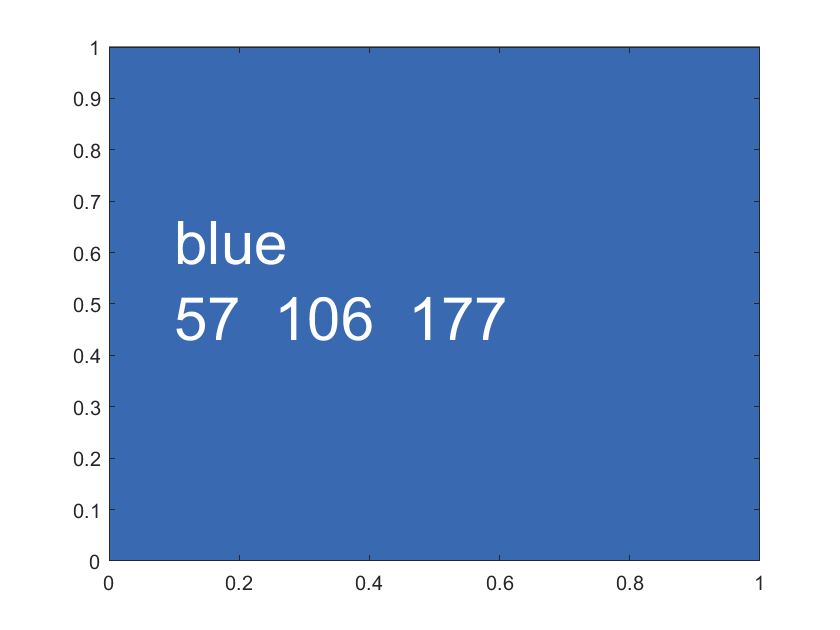
\includegraphics[width=5.20833in,height=\textheight]{img/fs_color_images/figure_0.png}

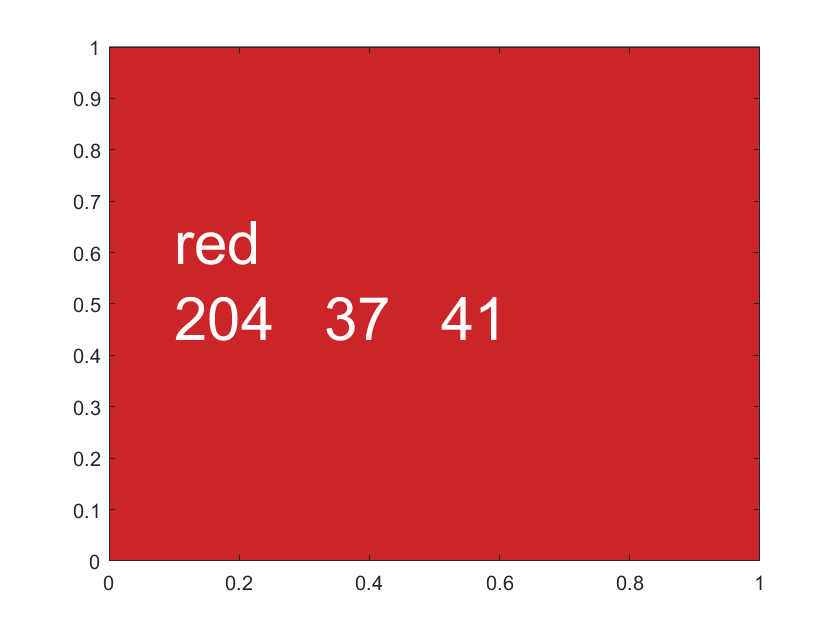
\includegraphics[width=5.20833in,height=\textheight]{img/fs_color_images/figure_1.png}

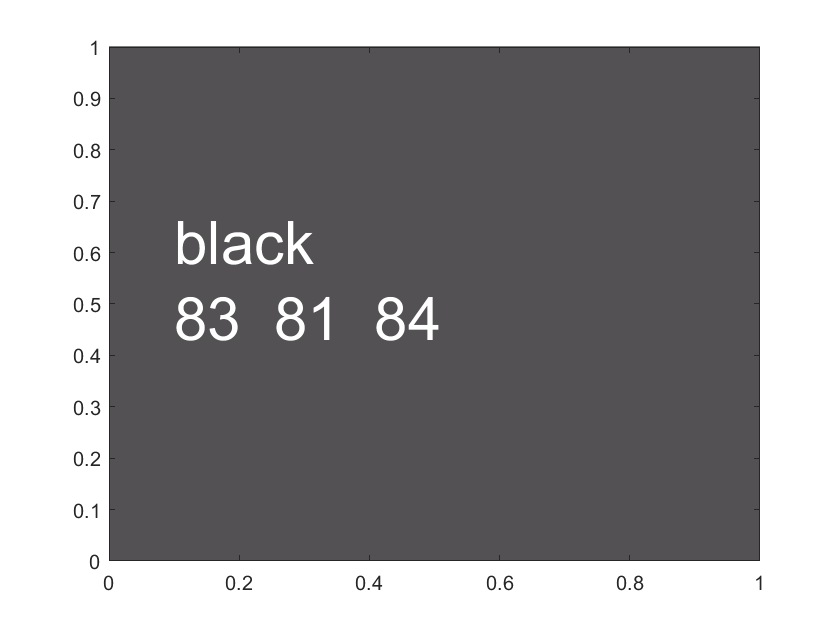
\includegraphics[width=5.20833in,height=\textheight]{img/fs_color_images/figure_2.png}

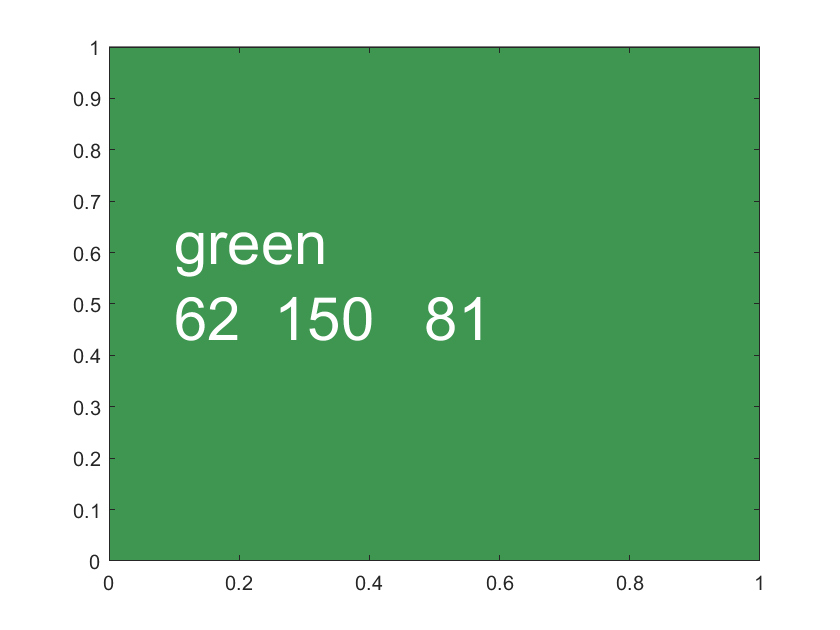
\includegraphics[width=5.20833in,height=\textheight]{img/fs_color_images/figure_3.png}

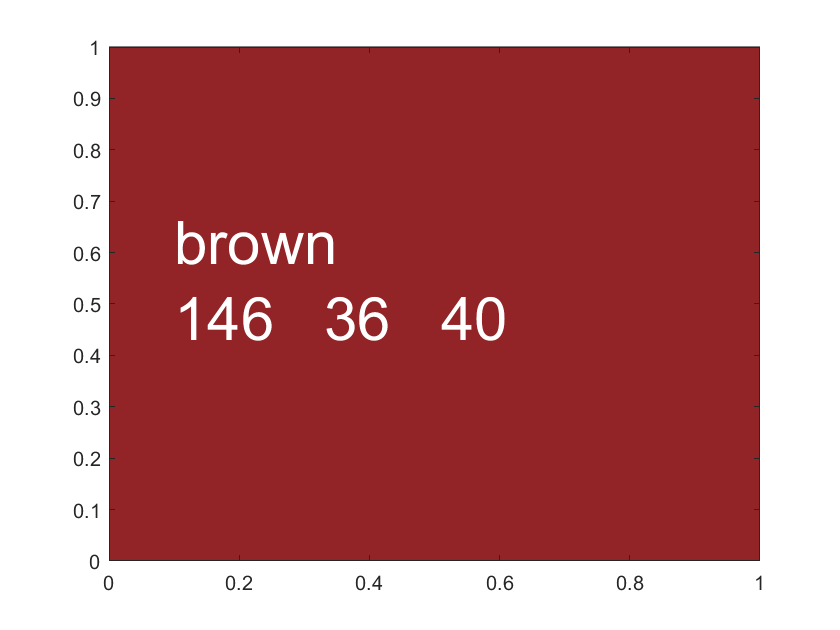
\includegraphics[width=5.20833in,height=\textheight]{img/fs_color_images/figure_4.png}

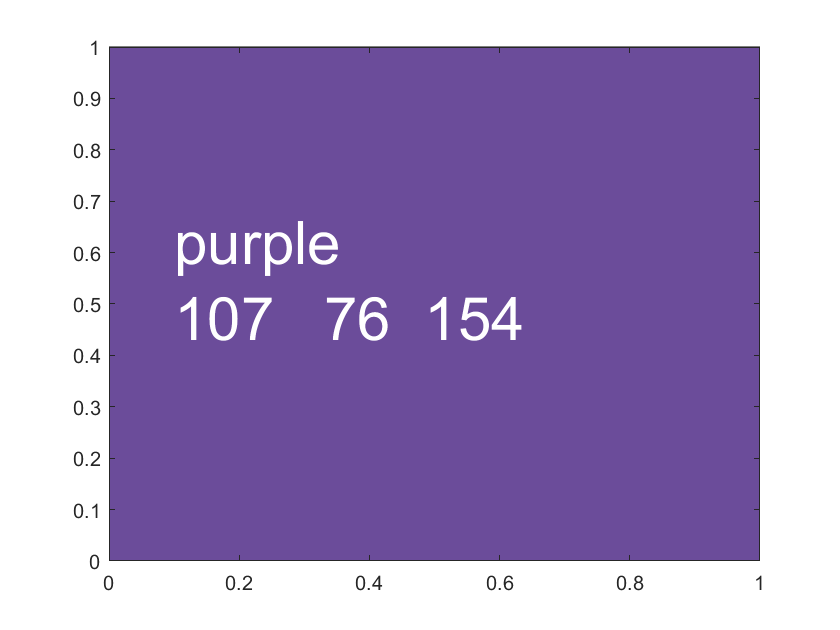
\includegraphics[width=5.20833in,height=\textheight]{img/fs_color_images/figure_5.png}

\hypertarget{good-colors-to-use-lighter}{%
\subsubsection{Good Colors to Use Lighter}\label{good-colors-to-use-lighter}}

Nice ligher colors to use in matlab.

\begin{verbatim}
close all

blue = [114 147 203]./255;
red = [211 94 96]./255;
black = [128 133 133]./255;
green = [132 186 91]./255;
brown = [171 104 87]./255;
purple = [144 103 167]./255;
cl_colors = {blue, red, black, ...
             green, brown, purple};
cl_str_clr_names = ["blue", "red", "black", "green", "brown", "purple"];

for it_color=1:length(cl_colors)
    
    figure();
    x = [0 1 1 0];
    y = [0 0 1 1];
    fill(x, y, cl_colors{it_color});
    
    st_text = [cl_str_clr_names(it_color) num2str(round(cl_colors{it_color}*255))];
    hText = text(.10,.55, st_text);
    hText.Color = 'white';
    hText.FontSize = 30; 
    snapnow;
    
end
\end{verbatim}

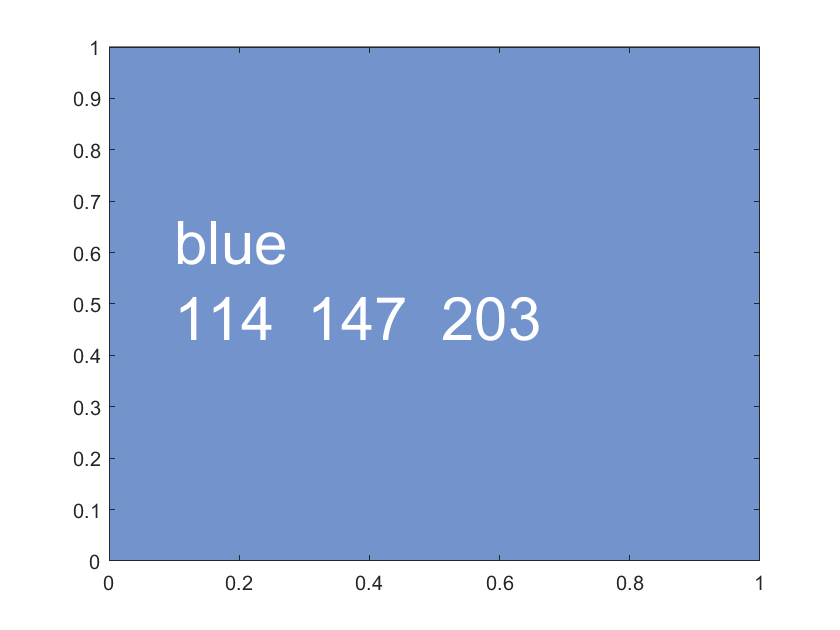
\includegraphics[width=5.20833in,height=\textheight]{img/fs_color_images/figure_6.png}

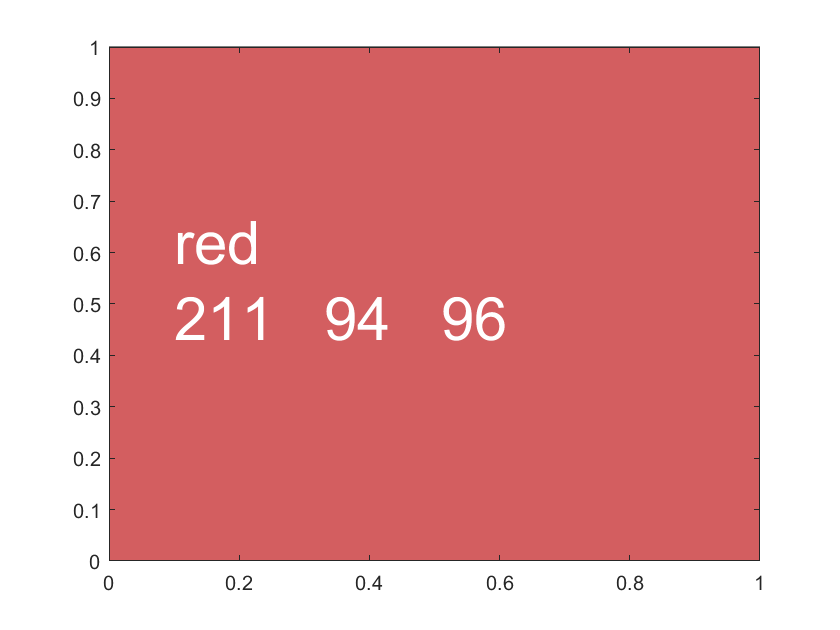
\includegraphics[width=5.20833in,height=\textheight]{img/fs_color_images/figure_7.png}

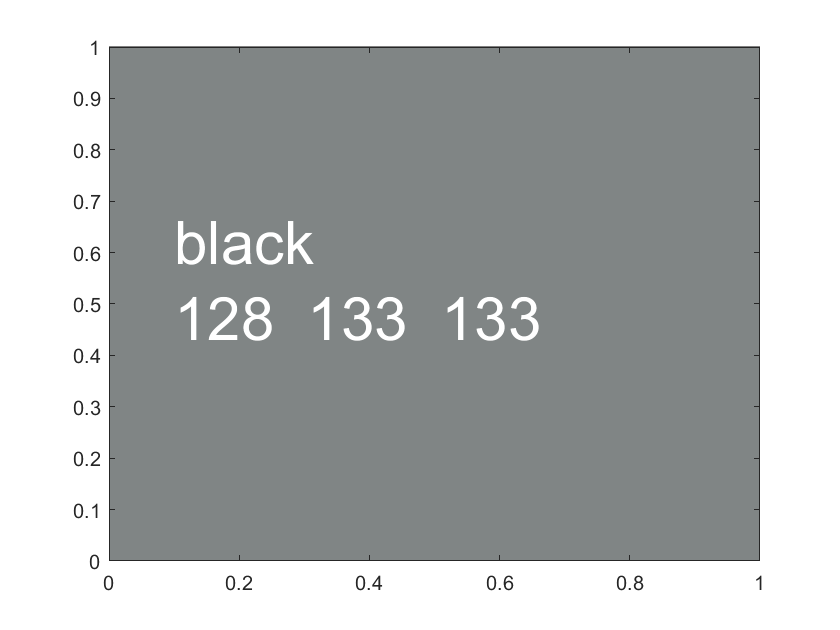
\includegraphics[width=5.20833in,height=\textheight]{img/fs_color_images/figure_8.png}

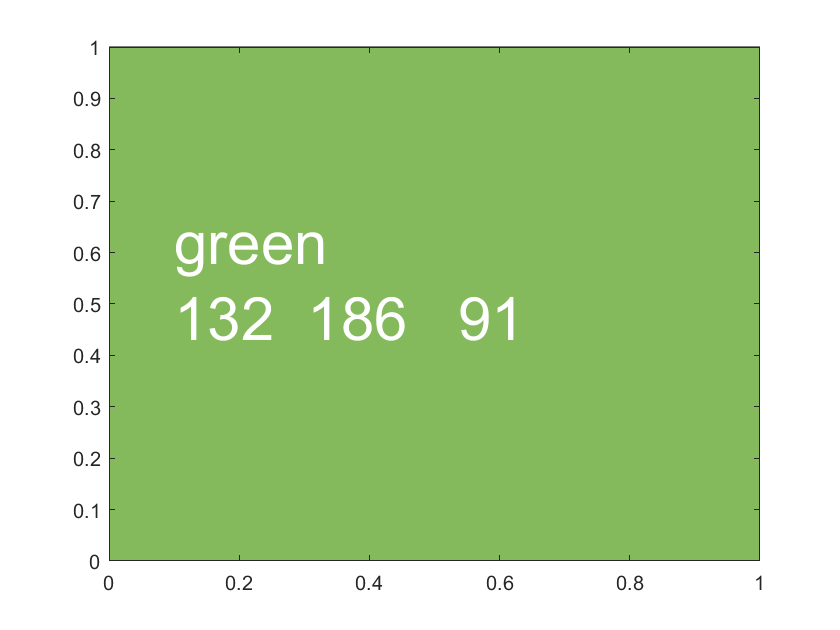
\includegraphics[width=5.20833in,height=\textheight]{img/fs_color_images/figure_9.png}

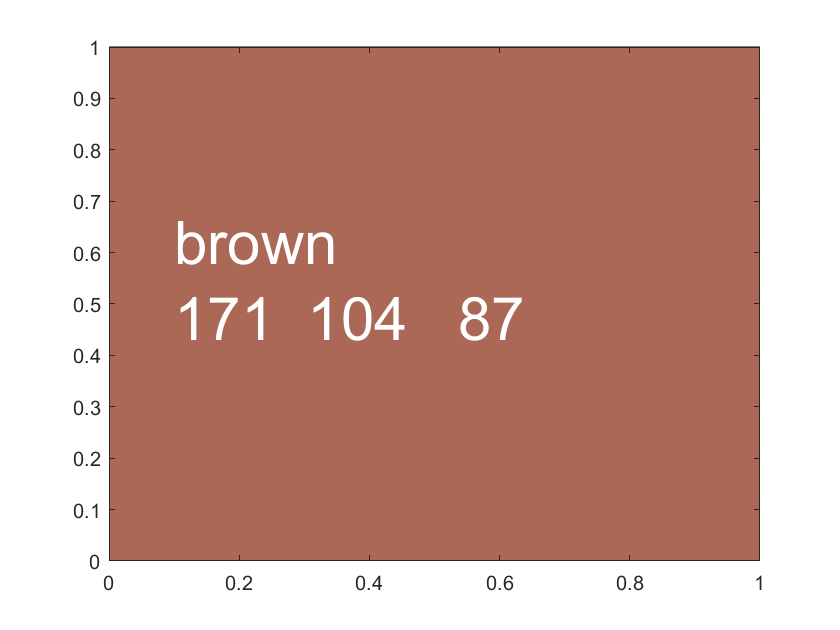
\includegraphics[width=5.20833in,height=\textheight]{img/fs_color_images/figure_10.png}

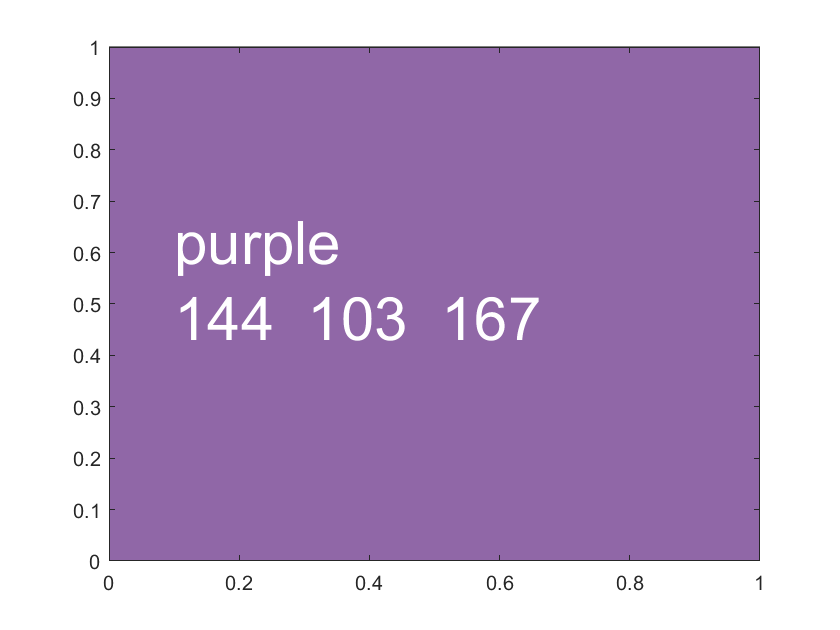
\includegraphics[width=5.20833in,height=\textheight]{img/fs_color_images/figure_11.png}

\hypertarget{matlab-has-a-graphical-tool-for-picking-color}{%
\subsubsection{Matlab has a graphical tool for picking color}\label{matlab-has-a-graphical-tool-for-picking-color}}

Enter uisetcolor pick color from new window and color values will appear
uisetcolor

\begin{verbatim}
% Color Pickers
% uisetcolor
\end{verbatim}

Picked Color use

\begin{verbatim}
figure();
hold on;

x = rand([10,1]);
y = rand([10,1]);

% Then can use for plot
plot(x,y,'Color',[.61 .51 .74]);

% Can use for Scatter
scatter(x, y, 10, ...
    'MarkerEdgeColor', [.61 .51 .74], 'MarkerFaceAlpha', 0.1, ...
    'MarkerFaceColor', [.61 .51 .74], 'MarkerEdgeAlpha', 0.1);
\end{verbatim}

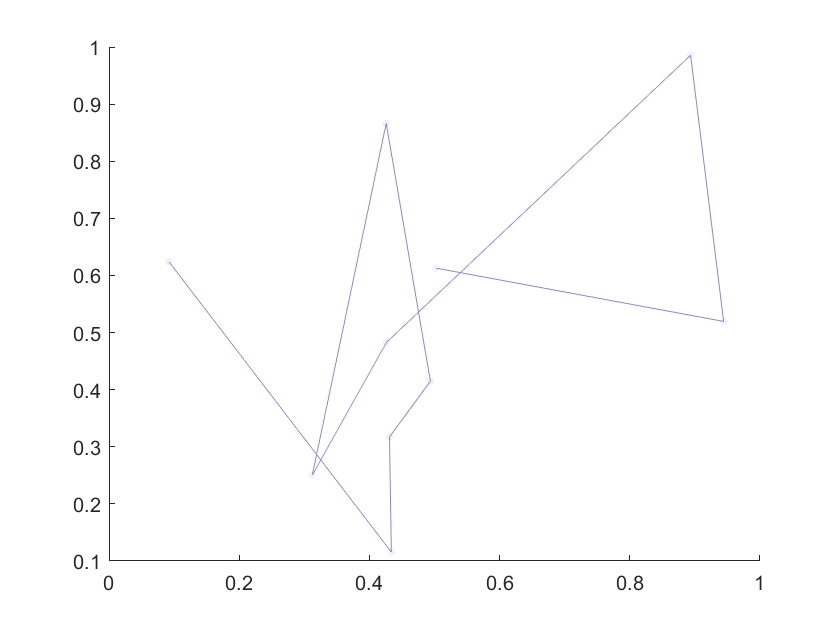
\includegraphics[width=5.20833in,height=\textheight]{img/fs_color_images/figure_12.png}

\hypertarget{matlab-graph-titling-labels-and-legends-examples}{%
\subsection{Matlab Graph Titling, Labels and Legends Examples}\label{matlab-graph-titling-labels-and-legends-examples}}

\begin{quote}
Go back to \href{http://fanwangecon.github.io/}{fan}'s \href{https://fanwangecon.github.io/MEconTools/}{MEconTools} Package, \href{https://fanwangecon.github.io/M4Econ/}{Matlab Code Examples} Repository (\href{https://fanwangecon.github.io/M4Econ/bookdown}{bookdown site}), or \href{https://fanwangecon.github.io/Math4Econ/}{Math for Econ with Matlab} Repository (\href{https://fanwangecon.github.io/Math4Econ/bookdown}{bookdown site}).
\end{quote}

\hypertarget{draw-a-figure-label-title-x-and-y-axises-with-latex-equations}{%
\subsubsection{\texorpdfstring{\textbf{Draw A figure Label Title, X and Y Axises with Latex Equations}}{Draw A figure Label Title, X and Y Axises with Latex Equations}}\label{draw-a-figure-label-title-x-and-y-axises-with-latex-equations}}

\begin{verbatim}
clear all;
close all;
figure();

% draw some lines
xline0 = xline(0);
xline0.HandleVisibility = 'off';
yline0 = yline(0);
yline0.HandleVisibility = 'off';
hline = refline([1 0]);
hline.Color = 'k';
hline.LineStyle = ':';
hline.HandleVisibility = 'off';

% Titling with multiple lines
title({'Cash-on-Hand given w(k+b),k,z' '$\alpha + \beta = \zeta$'},'Interpreter','latex');
ylabel({'Cash-on-Hand' 'line 2 $\frac{1}{2}$'},'Interpreter','latex');
xlabel({'Index of Cash-on-Hand Discrete Point'...
        ' $\frac{1}{2} + \alpha + \max + \sum_1^{B}$ Each Segment is a w=k+b; within segment increasing k'...
        'For each w and z, coh maximizing k is different'},'Interpreter','latex');
grid on;
grid minor;
\end{verbatim}

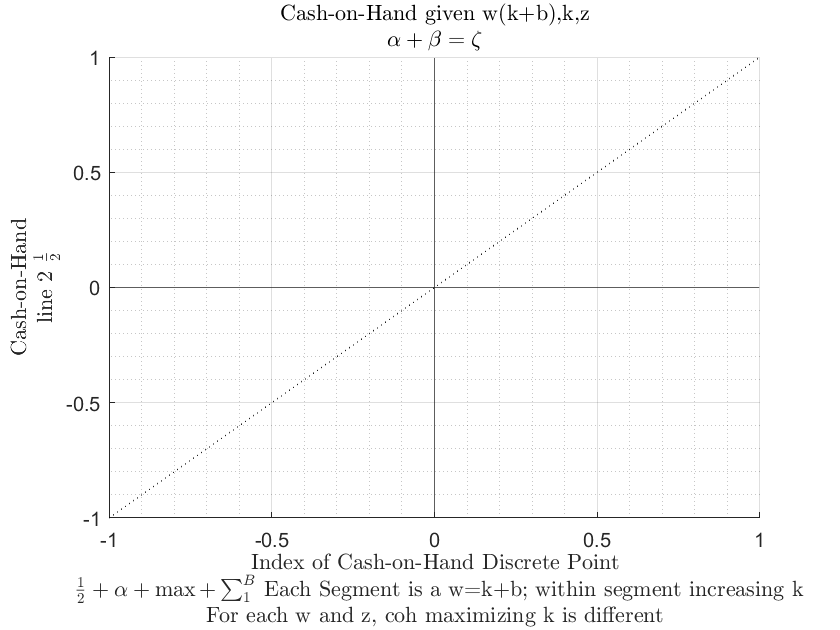
\includegraphics[width=5.20833in,height=\textheight]{img/fs_titling_images/figure_0.png}

\hypertarget{matlab-graph-specify-legends-manually}{%
\subsubsection{Matlab Graph Specify Legends Manually}\label{matlab-graph-specify-legends-manually}}

Specify labels manually, note we can use HandleVisibility to control
what part of figure show up in legends.

\begin{verbatim}
% Generate Random Data
rng(123);
it_x_n = 10;
it_x_groups_n = 3;
mat_y = rand([it_x_n, it_x_groups_n]);
mat_y = mat_y + sqrt(1:it_x_groups_n);
mat_y = mat_y + log(1:it_x_n)';
ar_x = 1:1:it_x_n;

% Start Figure
figure('PaperPosition', [0 0 10 10]);

hold on;

g1 = scatter(ar_x,  mat_y(:,1), 30, 'filled');
g2 = scatter(ar_x,  mat_y(:,2), 30, 'filled');
g3 = scatter(ar_x,  mat_y(:,3), 30, 'filled');

legend([g1, g2, g3], {'near','linear','spline'}, 'Location','best',...
        'NumColumns',1,'FontSize',12,'TextColor','black');

% PLot this line, but this line will not show up in legend
hline = refline([1 0]);
hline.Color = 'k';
hline.LineStyle = ':';
% not to show up in legend
hline.HandleVisibility = 'off';
grid on;
grid minor;

title(sprintf('griddedInterpolant comparison, crra utility approximation, interp grid n=%d', it_x_n))
ylabel('Actual Utility Evaluated at c')
xlabel('Approximated Util based on  Interpolation')
\end{verbatim}

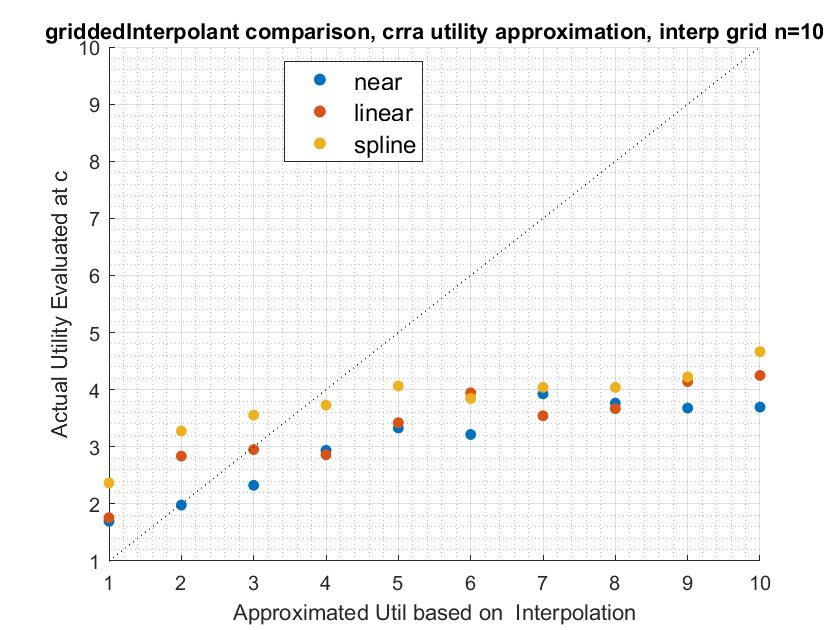
\includegraphics[width=5.20833in,height=\textheight]{img/fs_titling_images/figure_1.png}

\begin{verbatim}
snapnow;
\end{verbatim}

\hypertarget{given-graph-graph-subset-of-lines-and-add-extra-line-with-legend}{%
\subsubsection{Given Graph, Graph Subset of Lines and Add Extra Line with Legend}\label{given-graph-graph-subset-of-lines-and-add-extra-line-with-legend}}

Same plot as before, except we plot only 2 of the three lines and add
another line with associated legend entry.

\begin{verbatim}
legendCell = cellstr(num2str(ar_x', 'shock=%3.2f'));
xlinemax = xline(min(mat_y, [], 'all'));
xlinemax.Color = 'b';
xlinemax.LineWidth = 1.5;

legendCell{length(legendCell) + 1} = 'max-agg-save';
legend([g1, g3, xlinemax], legendCell([1,3,length(legendCell)]), 'Location', 'best');
\end{verbatim}

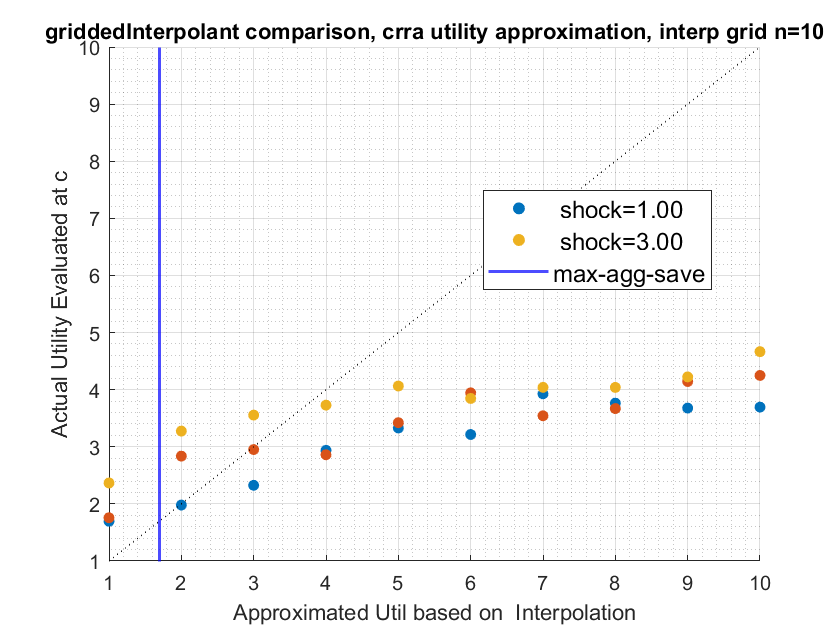
\includegraphics[width=5.20833in,height=\textheight]{img/fs_titling_images/figure_2.png}

\begin{verbatim}
snapnow;
\end{verbatim}

\hypertarget{matlab-graph-matrix-with-jet-spectrum-color-label-a-subset-examples}{%
\subsection{Matlab Graph Matrix with Jet Spectrum Color, Label a Subset Examples}\label{matlab-graph-matrix-with-jet-spectrum-color-label-a-subset-examples}}

\begin{quote}
Go back to \href{http://fanwangecon.github.io/}{fan}'s \href{https://fanwangecon.github.io/MEconTools/}{MEconTools} Package, \href{https://fanwangecon.github.io/M4Econ/}{Matlab Code Examples} Repository (\href{https://fanwangecon.github.io/M4Econ/bookdown}{bookdown site}), or \href{https://fanwangecon.github.io/Math4Econ/}{Math for Econ with Matlab} Repository (\href{https://fanwangecon.github.io/Math4Econ/bookdown}{bookdown site}).
\end{quote}

\hypertarget{plot-a-subset-of-data-matrix-with-appropriate-legends}{%
\subsubsection{Plot a Subset of Data Matrix with Appropriate Legends}\label{plot-a-subset-of-data-matrix-with-appropriate-legends}}

Sometimes we solve a model across many states, but we can only plot at a
subset of states, or perhaps we plot at all states, but only show
legends/labels for a subset.

In the example below, many lines are plotted, however, only a subset of
lines are labeled in the legend.

\begin{verbatim}
clear all;
close all;

% Generate Random Data
rng(123);
it_x_n = 10;
it_y_groups_n = 100;
ar_y = linspace(1,2,it_y_groups_n);
mat_y = rand([it_x_n, it_y_groups_n]);
mat_y = mat_y + sqrt(1:it_y_groups_n);
mat_y = mat_y + log(1:it_x_n)' + ar_y;
ar_x = 1:1:it_x_n;

% Jet color Graph All
figure('PaperPosition', [0 0 7 4]);
chart = plot(mat_y);
clr = jet(numel(chart));
for m = 1:numel(chart)
    set(chart(m),'Color',clr(m,:))
end

% zero lines
xline(0);
yline(0);

% invalid points separating lines
yline_borrbound = yline(3);
yline_borrbound.HandleVisibility = 'on';
yline_borrbound.LineStyle = ':';
yline_borrbound.Color = 'black';
yline_borrbound.LineWidth = 3;

% Titling
title('Cash-on-Hand given w(k+b),k,z');
ylabel('Cash-on-Hand');
xlabel({'Index of Cash-on-Hand Discrete Point'...
    'Each Segment is a w=k+b; within segment increasing k'...
    'For each w and z, coh maximizing k is different'});

% Xlim controls
xlim([min(ar_x), max(ar_x)]);

% Grid ons
grid on;
grid minor;
% Legends
legend2plot = fliplr([1 round(numel(chart)/3) round((2*numel(chart))/4)  numel(chart)]);
legendCell = cellstr(num2str(ar_y', 'shock=%3.2f'));

legendCell{length(legendCell) + 1} = 'borrow-constraint';
chart(length(chart)+1) = yline_borrbound;
legend(chart([legend2plot length(legendCell)]), ...
       legendCell([legend2plot length(legendCell)]), ...
       'Location', 'best');
\end{verbatim}

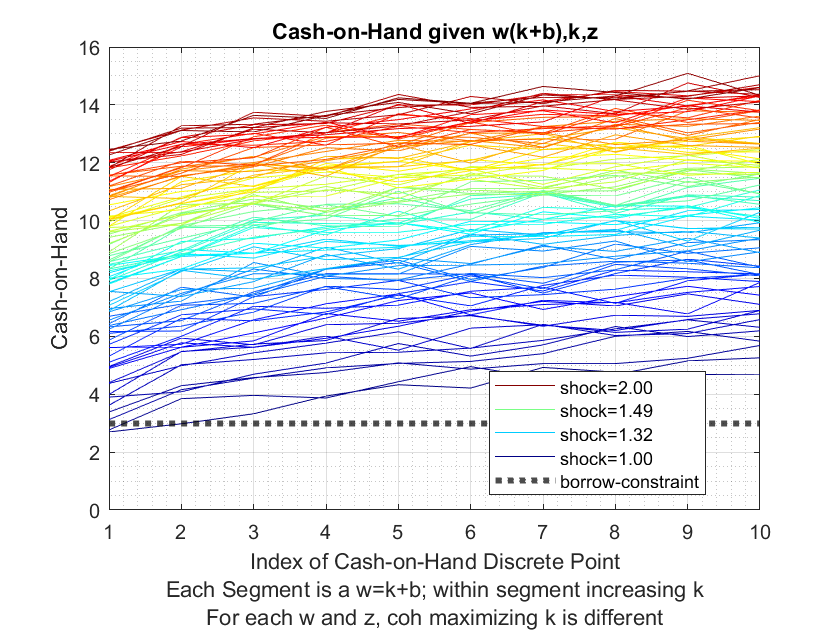
\includegraphics[width=5.20833in,height=\textheight]{img/fs_legendsubset_images/figure_0.png}

\hypertarget{basic-figure-types}{%
\section{Basic Figure Types}\label{basic-figure-types}}

\hypertarget{matlab-graph-scatter-plot-examples}{%
\subsection{Matlab Graph Scatter Plot Examples}\label{matlab-graph-scatter-plot-examples}}

\begin{quote}
Go back to \href{http://fanwangecon.github.io/}{fan}'s \href{https://fanwangecon.github.io/MEconTools/}{MEconTools} Package, \href{https://fanwangecon.github.io/M4Econ/}{Matlab Code Examples} Repository (\href{https://fanwangecon.github.io/M4Econ/bookdown}{bookdown site}), or \href{https://fanwangecon.github.io/Math4Econ/}{Math for Econ with Matlab} Repository (\href{https://fanwangecon.github.io/Math4Econ/bookdown}{bookdown site}).
\end{quote}

\hypertarget{scatter-plot-example}{%
\subsubsection{Scatter Plot Example}\label{scatter-plot-example}}

The plot below as square scatter points, each one with think border. Can
set transparency of border/edge and inside separately.

\begin{verbatim}
close all;
figure();
size = 100;
s = scatter(1:10,1:10,size);

s.Marker = 's';
% color picked by using: uisetcolor
s.MarkerEdgeColor = [0    0.4471    0.7412];
s.MarkerEdgeAlpha = 0.5;
s.MarkerFaceColor = [.61 .51 .74];
s.MarkerFaceAlpha = 1.0;
s.LineWidth = 10;
grid on;
grid minor;
\end{verbatim}

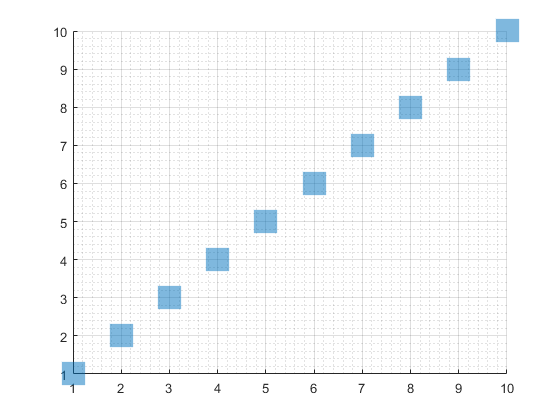
\includegraphics[width=5.20833in,height=\textheight]{img/fs_scatter_images/figure_0.png}

\begin{verbatim}
% 'o'   Circle
% '+'   Plus sign
% '*'   Asterisk
% '.'   Point
% 'x'   Cross
% 'square' or 's'   Square
% 'diamond' or 'd'  Diamond
% '^'   Upward-pointing triangle
% 'v'   Downward-pointing triangle
% '>'   Right-pointing triangle
% '<'   Left-pointing triangle
% 'pentagram' or 'p'    Five-pointed star (pentagram)
% 'hexagram' or 'h' Six-pointed star (hexagram)
% 'none'    No markers
\end{verbatim}

\hypertarget{scatter-with-edge-and-face-color-and-transparency}{%
\subsubsection{Scatter with Edge and Face Color and Transparency}\label{scatter-with-edge-and-face-color-and-transparency}}

Here is another way to Set Scatter Edge and Fac Colors and
Transparencies.

\begin{verbatim}
% Generate Data
rng(123);
it_x_n = 10;
it_x_groups_n = 3;
mat_y = rand([it_x_n, it_x_groups_n]);
mat_y = mat_y + sqrt(1:it_x_groups_n);
mat_y = mat_y + log(1:it_x_n)';
ar_x = 1:1:it_x_n;

% Colors
blue = [57 106 177]./255;
red = [204 37 41]./255;
black = [83 81 84]./255;
green = [62 150 81]./255;
brown = [146 36 40]./255;
purple = [107 76 154]./255;
cl_colors = {blue, red, black, ...
             green, brown, purple};

% Scatter Shapes
cl_scatter_shapes = {'s','x','o','d','p','*'};
% Scatter Sizes
cl_scatter_sizes = {100,100,50,50,50,50};
% Legend Keys
cl_legend = {'For Borr', 'Inf Borr', 'For+Inf Br'};

% Plot
figure();
hold on;
for it_m = 1:it_x_groups_n
    scatter(ar_x, mat_y(:,it_m), cl_scatter_sizes{it_m}, ...
        'Marker', cl_scatter_shapes{it_m}, ...
        'MarkerEdgeColor', cl_colors{it_m}, 'MarkerFaceAlpha', 0.8, ...
        'MarkerFaceColor', cl_colors{it_m}, 'MarkerEdgeAlpha', 0.8);
    cl_legend{it_m} = cl_legend{it_m};
end
legend(cl_legend, 'Location', 'best');
grid on; 
grid minor;
\end{verbatim}

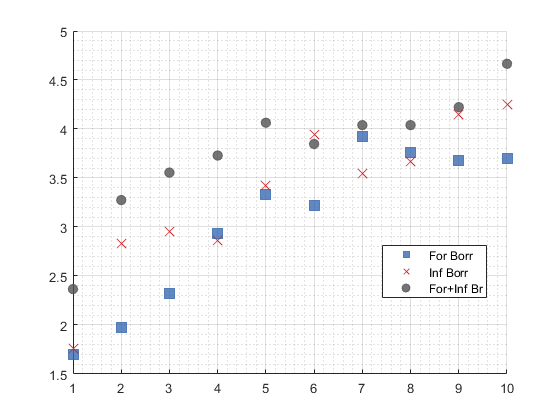
\includegraphics[width=5.20833in,height=\textheight]{img/fs_scatter_images/figure_1.png}

\hypertarget{matlab-line-and-scatter-plot-with-multiple-lines-and-axis-lines}{%
\subsection{Matlab Line and Scatter Plot with Multiple Lines and Axis Lines}\label{matlab-line-and-scatter-plot-with-multiple-lines-and-axis-lines}}

\begin{quote}
Go back to \href{http://fanwangecon.github.io/}{fan}'s \href{https://fanwangecon.github.io/MEconTools/}{MEconTools} Package, \href{https://fanwangecon.github.io/M4Econ/}{Matlab Code Examples} Repository (\href{https://fanwangecon.github.io/M4Econ/bookdown}{bookdown site}), or \href{https://fanwangecon.github.io/Math4Econ/}{Math for Econ with Matlab} Repository (\href{https://fanwangecon.github.io/Math4Econ/bookdown}{bookdown site}).
\end{quote}

\hypertarget{six-lines-plot}{%
\subsubsection{Six lines Plot}\label{six-lines-plot}}

Colors from \href{http://ksrowell.com/blog-visualizing-data/2012/02/02/optimal-colors-for-graphs/}{optimal
colors}.
Generate A line plot with multiple lines using safe colors, with
differening shapes. Figures include lines as well as scatter overlayed
jointly.

\begin{verbatim}
close all
figure();
hold on;

blue = [57 106 177]./255;
red = [204 37 41]./255;
black = [83 81 84]./255;
green = [62 150 81]./255;
brown = [146 36 40]./255;
purple = [107 76 154]./255;
cl_colors = {blue, red, black, ...
             green, brown, purple};
cl_legend = {'For Borr', 'Inf Borr', 'For+Inf Br', 'For+Br+Save', 'Bridge Loan', 'For Save'};
cl_scatter_shapes = {'s','x','o','d','p','*'};
cl_linestyle = {'--','-',':','-.','--','-'};
it_sca_bs = 20;
cl_scatter_csizes = {10*it_sca_bs, 20*it_sca_bs, 10*it_sca_bs, 10*it_sca_bs, 5*it_sca_bs, 8*it_sca_bs};
it_line_bs = 2;
cl_line_csizes = {1*it_line_bs, 2*it_line_bs, 1*it_line_bs, 1*it_line_bs, 1*it_line_bs, 2*it_line_bs};

it_x_groups_n = length(cl_scatter_csizes);
it_x_n = 10;

% Generate Random Data
rng(123);
mat_y = rand([it_x_n, it_x_groups_n]);
mat_y = mat_y + sqrt(1:it_x_groups_n);
mat_y = mat_y + log(1:it_x_n)';
ar_x = 1:1:it_x_n;

ar_it_graphs_run = 1:6;
it_graph_counter = 0;
ls_chart = [];
for it_fig = ar_it_graphs_run

    % Counter
    it_graph_counter = it_graph_counter + 1;

    % Y Outcome
    ar_y = mat_y(:, it_fig)';

    % Color and Size etc
    it_csize = cl_scatter_csizes{it_fig};
    ar_color = cl_colors{it_fig};
    st_shape = cl_scatter_shapes{it_fig};
    st_lnsty = cl_linestyle{it_fig};
    st_lnwth = cl_line_csizes{it_fig};
    
    % plot scatter and include in legend
    ls_chart(it_graph_counter) = scatter(ar_x, ar_y, it_csize, ar_color, st_shape);

    % plot line do not include in legend
    line = plot(ar_x, ar_y);
    line.HandleVisibility = 'off';
    line.Color = ar_color;
    line.LineStyle = st_lnsty;
    line.HandleVisibility = 'off';
    line.LineWidth = st_lnwth;

    % Legend to include
    cl_legend{it_graph_counter} = cl_legend{it_fig};
end

% Legend
legend(ls_chart, cl_legend, 'Location', 'southeast');

% labeling
title('Optimal Savings');
ylabel('Savings Levels');
xlabel('Cash-on-Hand Today');
grid on;
\end{verbatim}

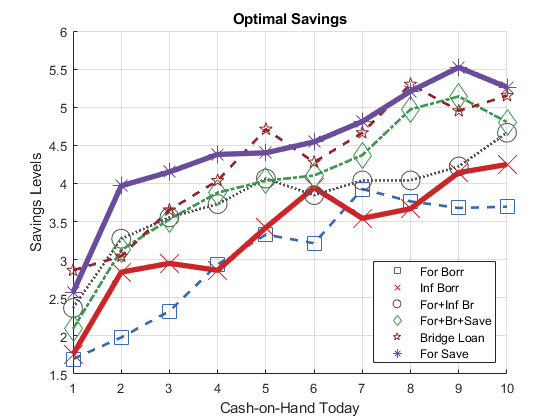
\includegraphics[width=5.20833in,height=\textheight]{img/fs_lines_images/figure_0.png}

\begin{verbatim}
snapnow;
\end{verbatim}

\hypertarget{horizontal-and-vertical-lines-and-45-degree}{%
\subsubsection{Horizontal and Vertical Lines and 45 Degree}\label{horizontal-and-vertical-lines-and-45-degree}}

Draw x and y axis, and draw a 45 degree line.

\begin{verbatim}
figure();

xline0 = xline(0);
xline0.HandleVisibility = 'off';
xline0.Color = red;
xline0.LineStyle = '--';
yline0 = yline(0);
yline0.HandleVisibility = 'off';
yline0.LineWidth = 1;

hline = refline([1 0]);
hline.Color = 'k';
hline.LineStyle = ':';
hline.HandleVisibility = 'off';

snapnow;
grid on;
grid minor;
\end{verbatim}

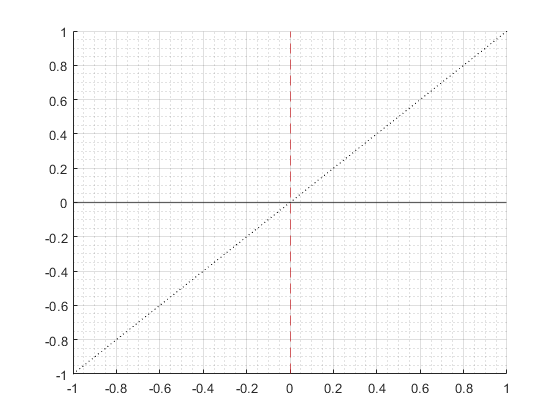
\includegraphics[width=5.20833in,height=\textheight]{img/fs_lines_images/figure_1.png}

\hypertarget{matlab-graph-scatter-and-line-spectrum-with-three-variables}{%
\subsection{Matlab Graph Scatter and Line Spectrum with Three Variables}\label{matlab-graph-scatter-and-line-spectrum-with-three-variables}}

\begin{quote}
Go back to \href{http://fanwangecon.github.io/}{fan}'s \href{https://fanwangecon.github.io/MEconTools/}{MEconTools} Package, \href{https://fanwangecon.github.io/M4Econ/}{Matlab Code Examples} Repository (\href{https://fanwangecon.github.io/M4Econ/bookdown}{bookdown site}), or \href{https://fanwangecon.github.io/Math4Econ/}{Math for Econ with Matlab} Repository (\href{https://fanwangecon.github.io/Math4Econ/bookdown}{bookdown site}).
\end{quote}

Generate k + b = w, color for each w, vectors of k and b such that k + b
= w for each w

There are two N by M matrix, A anb B.

Values in Matrix A correspond to the x-axis, values in Matrix B
correspond to the y-axis.

The rows and columns in matrix A and B have some other meanings. In this
case, we will give color to the columns.

The columns is represented by vector C, which is another variable.

\begin{enumerate}
\def\labelenumi{\arabic{enumi}.}
\item
  Each line a different color representing variable 3
\item
  Legend labeling a subset of colors
\item
  X and Y could be asset choices, color could be utility, consumption
  etc.
\end{enumerate}

\hypertarget{setting-up-data}{%
\subsubsection{Setting Up Data}\label{setting-up-data}}

\begin{verbatim}
close all
clear all

% Bounds
fl_b_bd = -10;
% Max and Mins
fl_w_max = 50;
fl_w_min = fl_b_bd;
fl_kp_max = fl_w_max - fl_b_bd;
fl_kp_min = 0;

% Grid Point Counts
it_w_i = 30;
it_kb_j = 30;

% Grids
ar_w = linspace(fl_w_min, fl_w_max, it_w_i);
ar_kp = linspace(fl_kp_min, fl_kp_max, it_kb_j);
mt_bp = ar_w - ar_kp';
mt_kp = ar_w - mt_bp;
mt_bl_constrained = (mt_bp < fl_b_bd);
mt_bp_wth_na = mt_bp;
mt_kp_wth_na = mt_kp;
mt_bp_wth_na(mt_bl_constrained) = nan;
mt_kp_wth_na(mt_bl_constrained) = nan;

% Flatten
ar_bp_mw_wth_na = mt_bp_wth_na(:);
ar_kp_mw_wth_na = mt_kp_wth_na(:);
ar_bp_mw = ar_bp_mw_wth_na(~isnan(ar_bp_mw_wth_na));
ar_kp_mw = ar_kp_mw_wth_na(~isnan(ar_kp_mw_wth_na));
\end{verbatim}

\hypertarget{graphing}{%
\subsubsection{Graphing}\label{graphing}}

\begin{verbatim}
figure('PaperPosition', [0 0 7 4]);
hold on;

chart = plot(mt_bp_wth_na, mt_kp_wth_na, 'blue');

clr = jet(numel(chart));
for m = 1:numel(chart)
   set(chart(m),'Color',clr(m,:))
end
if (length(ar_w) <= 50) 
    scatter(ar_bp_mw, ar_kp_mw, 5, 'filled');
end
xline(0);
yline(0);

title('Choice Grids Conditional on kp+bp=w')
ylabel('Capital Choice')
xlabel({'Borrowing or Saving'})
legend2plot = fliplr([1 round(numel(chart)/3) round((2*numel(chart))/4)  numel(chart)]);
legendCell = cellstr(num2str(ar_w', 'kp+bp=%3.2f'));
legend(chart(legend2plot), legendCell(legend2plot), 'Location','northeast');

grid on;
\end{verbatim}

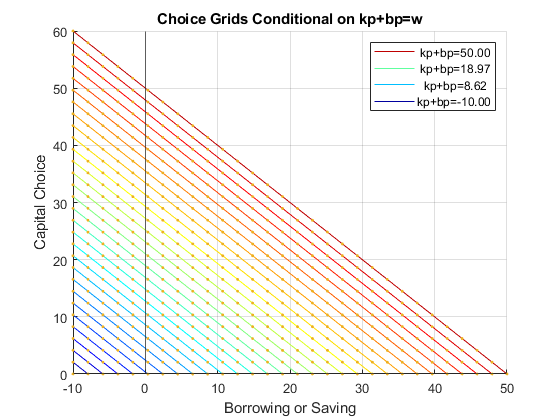
\includegraphics[width=5.20833in,height=\textheight]{img/fs_specline_images/figure_0.png}

\hypertarget{graph-functions}{%
\section{Graph Functions}\label{graph-functions}}

\hypertarget{matlab-graph-one-variable-function}{%
\subsection{Matlab Graph One Variable Function}\label{matlab-graph-one-variable-function}}

\begin{quote}
Go back to \href{http://fanwangecon.github.io/}{fan}'s \href{https://fanwangecon.github.io/MEconTools/}{MEconTools} Package, \href{https://fanwangecon.github.io/M4Econ/}{Matlab Code Examples} Repository (\href{https://fanwangecon.github.io/M4Econ/bookdown}{bookdown site}), or \href{https://fanwangecon.github.io/Math4Econ/}{Math for Econ with Matlab} Repository (\href{https://fanwangecon.github.io/Math4Econ/bookdown}{bookdown site}).
\end{quote}

\hypertarget{fplot-a-function-of-x}{%
\subsubsection{fplot a Function of X}\label{fplot-a-function-of-x}}

Given a cubic (polynomial) function, graph it using the fplot function,
between some values along the domain of the function. This function is
defined everywhere along the real-line. Note that fplot automatically
resizes the y-scale to show the full plot clearly.

\begin{verbatim}
% close all
figure();
hold on;

% Define a function
syms x
f_x = -7*x^(3);

% Set bounds on the domain
fl_x_lower = -2;
fl_x_higher = 2;

% Graph
fplot(f_x, [fl_x_lower, fl_x_higher])

% Add x-axis and y-axis
xline(0);
yline(0);

% Title and y and y-able
title(['Plot function: ' char(f_x)],'Interpreter',"none");
ylabel('f(x)');
xlabel('x');

% Add grids
grid on;
grid minor;
\end{verbatim}

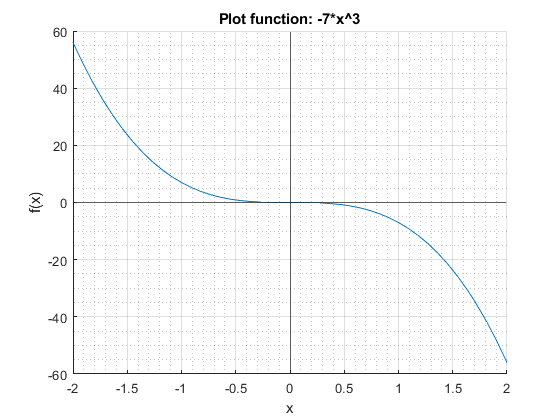
\includegraphics[width=5.20833in,height=\textheight]{img/fs_fplot_images/figure_0.png}

Plot a rational function, that is a function of polynomials.

\begin{verbatim}
% close all
figure();
hold on;

% Define a function
syms x
f_x = (x)/(x^2 + 1);

% Set bounds on the domain
fl_x_lower = -2;
fl_x_higher = 2;

% Graph
fplot(f_x, [fl_x_lower, fl_x_higher])

% Add x-axis and y-axis
xline(0);
yline(0);

% Title and y and y-able
title(['Plot function: ' char(f_x)],'Interpreter',"none");
ylabel('f(x)');
xlabel('x');

% Add grids
grid on;
grid minor;
\end{verbatim}

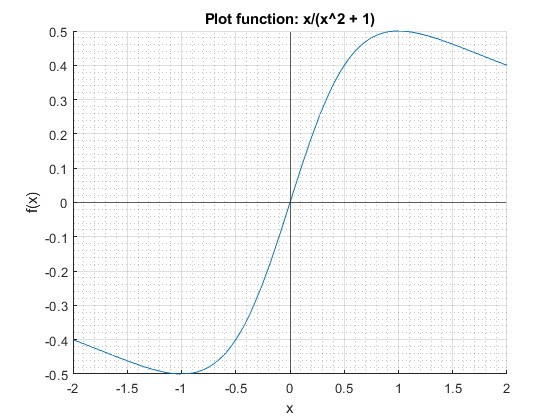
\includegraphics[width=5.20833in,height=\textheight]{img/fs_fplot_images/figure_1.png}

Plot a function that is not defined at all points along the real line.
Note also that the function always returns a positive value. Note the
fplot function automatically identifies the part of the x-axis where the
function is not defined, and draws dashed lines to demarcate.

\begin{verbatim}
% close all
figure();
hold on;

% Define a function
syms x
f_x = 5*(x^5 - 6*x^2 + 3*x)^(2/3);

% Set bounds on the domain
fl_x_lower = -1;
fl_x_higher = 2;

% Graph
fplot(f_x, [fl_x_lower, fl_x_higher])

% Add x-axis and y-axis
xline(0);
yline(0);

% Title and y and y-able
title(['Plot function: ' char(f_x)],'Interpreter',"none");
ylabel('f(x)');
xlabel('x');

% Add grids
grid on;
grid minor;
\end{verbatim}

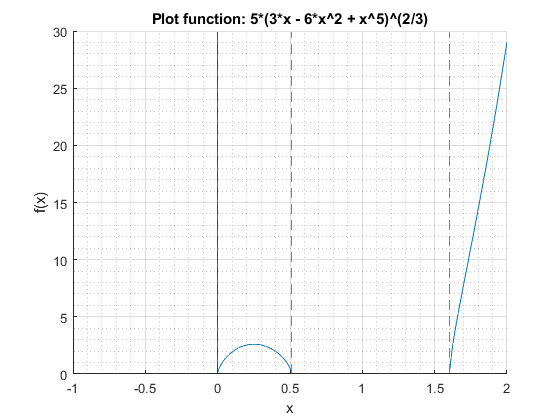
\includegraphics[width=5.20833in,height=\textheight]{img/fs_fplot_images/figure_2.png}

\hypertarget{plot-indifference-curve-and-budget-constraint}{%
\subsubsection{Plot Indifference Curve and Budget Constraint}\label{plot-indifference-curve-and-budget-constraint}}

Indifference curve and two budget lines. From \href{https://fanwangecon.github.io/Math4Econ/derivative_application/htmlpdfm/K_save_households.html}{two period consumption
and savings
problem}.

\begin{verbatim}
% close all
figure();
hold on;

% Define parameters
e1 = 1.5;
e2 = 1.9;
r = 0.05;

u_star = 1.5;
beta = 0.9;

% Define a function
% x = c1, f_x = c2
syms x
f_x_indiff = exp((u_star - log(x))/beta);

% Formula for optimal choice that minimize expenditure
c2_star_exp_min = exp((u_star + log(beta*(1+r)))/(1+beta));
c1_star_exp_min = (1/(beta*(1+r)))*c2_star_exp_min;
f_optimal_cost = c1_star_exp_min*(1+r)+c2_star_exp_min;

% budget equation
% x = c1, f_x = y
f_x_budget = (e1*(1+r) + e2) + (-1)*(1+r)*x;
f_x_budget_optimal_cost = f_optimal_cost + (-1)*(1+r)*x;

% Set bounds on the domain
fl_x_lower = 0;
fl_x_higher = 6;

% Graph
hold on;
fplot(f_x_indiff, [fl_x_lower, fl_x_higher])
fplot(f_x_budget, [fl_x_lower, fl_x_higher])
fplot(f_x_budget_optimal_cost, [fl_x_lower, fl_x_higher])

% plot a one point scatter plot
scatter(c1_star_exp_min, c2_star_exp_min, 300, 'filled');

% Add x-axis and y-axis
xline(0);
yline(0);

% Title and y and y-able
title(['Plot function: ' char(f_x_indiff)],'Interpreter',"none");
ylabel('c2');
xlabel('c1');

% this sets x and y visual boundaries
ylim([0,6]);
xlim([0,6]);
% Add grids
grid on;
grid minor;
\end{verbatim}

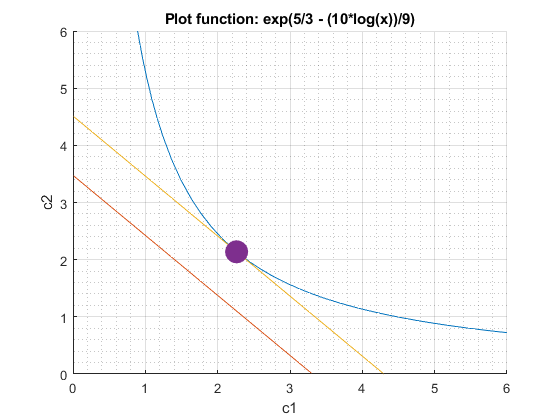
\includegraphics[width=5.20833in,height=\textheight]{img/fs_fplot_images/figure_3.png}

\hypertarget{write-and-read-plots}{%
\section{Write and Read Plots}\label{write-and-read-plots}}

\hypertarget{matlab-graph-generate-eps-postscript-figures-in-matlab}{%
\subsection{Matlab Graph Generate EPS postscript figures in matlab}\label{matlab-graph-generate-eps-postscript-figures-in-matlab}}

\begin{quote}
Go back to \href{http://fanwangecon.github.io/}{fan}'s \href{https://fanwangecon.github.io/MEconTools/}{MEconTools} Package, \href{https://fanwangecon.github.io/M4Econ/}{Matlab Code Examples} Repository (\href{https://fanwangecon.github.io/M4Econ/bookdown}{bookdown site}), or \href{https://fanwangecon.github.io/Math4Econ/}{Math for Econ with Matlab} Repository (\href{https://fanwangecon.github.io/Math4Econ/bookdown}{bookdown site}).
\end{quote}

\hypertarget{properly-save-eps-with-scatter-and-other-graphing-methods-renderer-painters}{%
\subsubsection{Properly Save EPS with Scatter and Other Graphing Methods: Renderer = Painters}\label{properly-save-eps-with-scatter-and-other-graphing-methods-renderer-painters}}

scatter plot saving as eps seems to only work when Renderer is set to
Painters

\begin{verbatim}
fl_fig_wdt = 3;
fl_fig_hgt = 2.65;

figure('PaperPosition', [0 0 fl_fig_wdt fl_fig_hgt], 'Renderer', 'Painters');
x = rand([10,1]);
y = rand([10,1]);
scatter(x, y, 'filled');
grid on;
grid minor;

st_img_path = 'C:/Users/fan/M4Econ/graph/export/_img/';
st_file_name = 'fs_eps_scatter_test';

% eps figure save with tiff preview
print(strcat(st_img_path, st_file_name), '-depsc', '-tiff');
\end{verbatim}

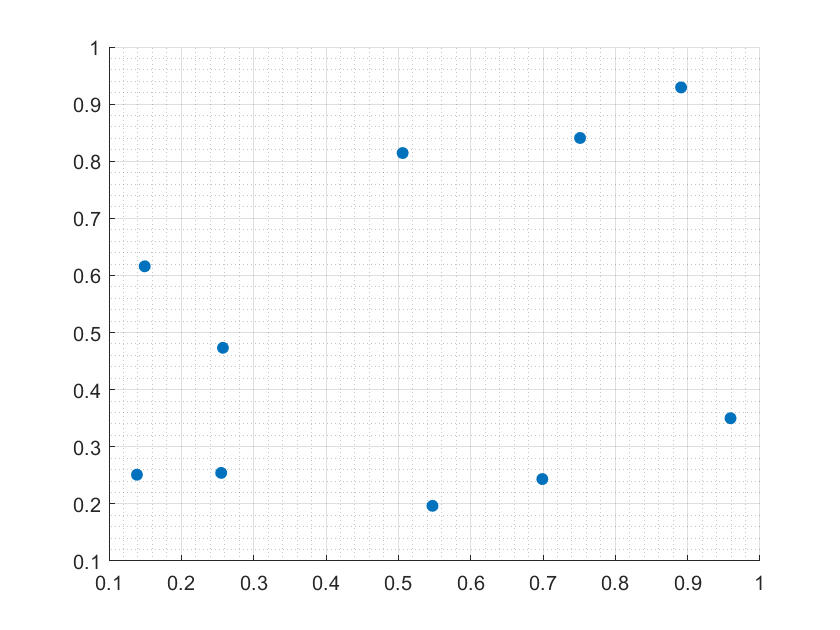
\includegraphics[width=5.20833in,height=\textheight]{img/fs_eps_images/figure_0.png}

\hypertarget{tables}{%
\chapter{Tables}\label{tables}}

\hypertarget{basic-table-generation}{%
\section{Basic Table Generation}\label{basic-table-generation}}

\hypertarget{named-tables-with-random-data}{%
\subsection{Named Tables with Random Data}\label{named-tables-with-random-data}}

\begin{quote}
Go back to \href{http://fanwangecon.github.io/}{fan}'s \href{https://fanwangecon.github.io/MEconTools/}{MEconTools} Package, \href{https://fanwangecon.github.io/M4Econ/}{Matlab Code Examples} Repository (\href{https://fanwangecon.github.io/M4Econ/bookdown}{bookdown site}), or \href{https://fanwangecon.github.io/Math4Econ/}{Math for Econ with Matlab} Repository (\href{https://fanwangecon.github.io/Math4Econ/bookdown}{bookdown site}).
\end{quote}

\hypertarget{generate-a-table-with-m-variables}{%
\subsubsection{Generate A Table with M Variables}\label{generate-a-table-with-m-variables}}

Generate a numeric table with random varlues and a string column

\begin{verbatim}
% Numeric Matrix
it_num_cols = 4;
it_num_rows = 5;
mt_data = rand([it_num_rows, it_num_cols]);

% Generate Table
tb_test = array2table(mt_data);

% Generate Row and Column Names
cl_col_names = strcat('col_', string((1:it_num_cols)));
cl_row_names = strcat('row_', string((1:it_num_rows)));

tb_test.Properties.VariableNames = matlab.lang.makeValidName(cl_col_names);
tb_test.Properties.RowNames = matlab.lang.makeValidName(cl_row_names);

% Generate two string variable
rng(456);
cl_st_var1 = strcat('data=', string(rand([it_num_rows,1])));
cl_st_var2 = strcat('data=', string(rand([it_num_rows,1])));
tb_test = addvars(tb_test, cl_st_var1, cl_st_var2);

% Display Table
disp(tb_test);

              col_1      col_2       col_3       col_4       cl_st_var1        cl_st_var2  
             _______    _______    _________    _______    ______________    ______________

    row_1    0.43568     0.4688      0.18092    0.14604    "data=0.24876"    "data=0.60411"
    row_2    0.38527       0.57      0.11816    0.54272    "data=0.16307"    "data=0.8857" 
    row_3    0.57571     0.6457      0.24273     0.8571    "data=0.78364"    "data=0.75912"
    row_4    0.14609    0.72334    0.0081834    0.20021    "data=0.80852"    "data=0.18111"
    row_5    0.68659    0.68067      0.36007    0.13463    "data=0.62563"    "data=0.15017"
\end{verbatim}

\hypertarget{tables-order-sort-add-rename-and-drop-columns}{%
\subsection{Tables Order, Sort, Add, Rename and Drop Columns}\label{tables-order-sort-add-rename-and-drop-columns}}

\begin{quote}
Go back to \href{http://fanwangecon.github.io/}{fan}'s \href{https://fanwangecon.github.io/MEconTools/}{MEconTools} Package, \href{https://fanwangecon.github.io/M4Econ/}{Matlab Code Examples} Repository (\href{https://fanwangecon.github.io/M4Econ/bookdown}{bookdown site}), or \href{https://fanwangecon.github.io/Math4Econ/}{Math for Econ with Matlab} Repository (\href{https://fanwangecon.github.io/Math4Econ/bookdown}{bookdown site}).
\end{quote}

\hypertarget{given-table-show-some-columns-first}{%
\subsubsection{Given Table, Show Some Columns First}\label{given-table-show-some-columns-first}}

\begin{verbatim}
% Generate Table
it_num_cols = 4;
it_num_rows = 5;
mt_data = rand([it_num_rows, it_num_cols]);
tb_test = array2table(mt_data);
cl_col_names = strcat('col_', string((1:it_num_cols)));
cl_row_names = strcat('row_', string((1:it_num_rows)));
tb_test.Properties.VariableNames = matlab.lang.makeValidName(cl_col_names);
tb_test.Properties.RowNames = matlab.lang.makeValidName(cl_row_names);

rng(123);
mean = strcat('data=', string(rand([it_num_rows,1])));
sd = strcat('data=', string(rand([it_num_rows,1])));
tb_test_ori = addvars(tb_test, mean, sd);

% Move Variable
tb_test_varmove = movevars(tb_test_ori, {'mean', 'sd'}, 'Before', 'col_1');

% Display
disp(tb_test_ori);

              col_1       col_2      col_3      col_4          mean               sd      
             ________    _______    _______    _______    ______________    ______________

    row_1     0.34318      0.738     0.6344    0.32296    "data=0.69647"    "data=0.42311"
    row_2     0.72905    0.18249    0.84943    0.36179    "data=0.28614"    "data=0.98076"
    row_3     0.43857    0.17545    0.72446    0.22826    "data=0.22685"    "data=0.68483"
    row_4    0.059678    0.53155    0.61102    0.29371    "data=0.55131"    "data=0.48093"
    row_5     0.39804    0.53183    0.72244    0.63098    "data=0.71947"    "data=0.39212"

disp(tb_test_varmove);

                  mean               sd           col_1       col_2      col_3      col_4 
             ______________    ______________    ________    _______    _______    _______

    row_1    "data=0.69647"    "data=0.42311"     0.34318      0.738     0.6344    0.32296
    row_2    "data=0.28614"    "data=0.98076"     0.72905    0.18249    0.84943    0.36179
    row_3    "data=0.22685"    "data=0.68483"     0.43857    0.17545    0.72446    0.22826
    row_4    "data=0.55131"    "data=0.48093"    0.059678    0.53155    0.61102    0.29371
    row_5    "data=0.71947"    "data=0.39212"     0.39804    0.53183    0.72244    0.63098
\end{verbatim}

\hypertarget{rename-table-columns}{%
\subsubsection{Rename Table Columns}\label{rename-table-columns}}

Rename the first Column, rename the `sd' column, then rename the 3rd and
4th Columns. Note for multiple column renaming, use parenthesis, but for
single column renaming, use bracket.

\begin{verbatim}
tb_test_varmove.Properties.VariableNames{1} = 'RenameMean';
tb_test_varmove.Properties.VariableNames{'sd'} = 'RenameSDCol';
tb_test_varmove.Properties.VariableNames([3 4]) = {'3rd' '4th'};
disp(tb_test_varmove);

               RenameMean       RenameSDCol        3rd         4th       col_3      col_4 
             ______________    ______________    ________    _______    _______    _______

    row_1    "data=0.69647"    "data=0.42311"     0.34318      0.738     0.6344    0.32296
    row_2    "data=0.28614"    "data=0.98076"     0.72905    0.18249    0.84943    0.36179
    row_3    "data=0.22685"    "data=0.68483"     0.43857    0.17545    0.72446    0.22826
    row_4    "data=0.55131"    "data=0.48093"    0.059678    0.53155    0.61102    0.29371
    row_5    "data=0.71947"    "data=0.39212"     0.39804    0.53183    0.72244    0.63098
\end{verbatim}

\hypertarget{remove-table-column}{%
\subsubsection{\texorpdfstring{\texttt{Remove\ Table\ Column}}{Remove Table Column}}\label{remove-table-column}}

\texttt{Remove\ columns\ from\ the\ Table}

\begin{verbatim}
tb_test_varmove_drop = removevars(tb_test_varmove, {'3rd', 'col_3'});
disp(tb_test_varmove_drop);

               RenameMean       RenameSDCol        4th       col_4 
             ______________    ______________    _______    _______

    row_1    "data=0.69647"    "data=0.42311"      0.738    0.32296
    row_2    "data=0.28614"    "data=0.98076"    0.18249    0.36179
    row_3    "data=0.22685"    "data=0.68483"    0.17545    0.22826
    row_4    "data=0.55131"    "data=0.48093"    0.53155    0.29371
    row_5    "data=0.71947"    "data=0.39212"    0.53183    0.63098
\end{verbatim}

\hypertarget{row-and-column-names-for-table-based-on-arrays}{%
\subsection{Row and Column Names for Table based on Arrays}\label{row-and-column-names-for-table-based-on-arrays}}

\begin{quote}
Go back to \href{http://fanwangecon.github.io/}{fan}'s \href{https://fanwangecon.github.io/MEconTools/}{MEconTools} Package, \href{https://fanwangecon.github.io/M4Econ/}{Matlab Code Examples} Repository (\href{https://fanwangecon.github.io/M4Econ/bookdown}{bookdown site}), or \href{https://fanwangecon.github.io/Math4Econ/}{Math for Econ with Matlab} Repository (\href{https://fanwangecon.github.io/Math4Econ/bookdown}{bookdown site}).
\end{quote}

\hypertarget{generate-table-with-row-and-column-names-based-on-multiple-numeric-array}{%
\subsubsection{Generate Table with Row and Column Names based on Multiple Numeric Array}\label{generate-table-with-row-and-column-names-based-on-multiple-numeric-array}}

Two numeric arrays describe the column names, combine numeric arrays
together to form string array which becomes table variable/column names.

\begin{verbatim}
close all;

% Generate Table 1
ar_fl_abc1 = [0.4 0.1 0.25 0.3 0.4];
ar_fl_abc2 = [0.4 0.1 0.2 0.3 0.4];
number1 = '123';
number2 = '456';
mt_data_a = [ar_fl_abc1' ar_fl_abc2'];

tb_test_a = array2table(mt_data_a);
cl_col_names_a = {['col' num2str(number1)], ['col' num2str(number2)]};
cl_row_names_a = strcat('rowA=', string((1:size(mt_data_a,1))));

tb_test_a.Properties.VariableNames = cl_col_names_a;
tb_test_a.Properties.RowNames = cl_row_names_a;
disp(tb_test_a);

              col123    col456
              ______    ______

    rowA=1      0.4      0.4  
    rowA=2      0.1      0.1  
    rowA=3     0.25      0.2  
    rowA=4      0.3      0.3  
    rowA=5      0.4      0.4  
\end{verbatim}

\hypertarget{include-row-names-as-a-a-string-cell-variable}{%
\subsubsection{Include Row Names as a a String Cell Variable}\label{include-row-names-as-a-a-string-cell-variable}}

\begin{verbatim}
% a and b must have the same row names
cl_st_varrownames = tb_test_a.Properties.RowNames;
tb_test_a = addvars(tb_test_a, cl_st_varrownames, 'Before', 1);

disp(tb_test_a);

              cl_st_varrownames    col123    col456
              _________________    ______    ______

    rowA=1       {'rowA=1'}          0.4      0.4  
    rowA=2       {'rowA=2'}          0.1      0.1  
    rowA=3       {'rowA=3'}         0.25      0.2  
    rowA=4       {'rowA=4'}          0.3      0.3  
    rowA=5       {'rowA=5'}          0.4      0.4  
\end{verbatim}

\hypertarget{include-row-names-as-a-string-variable}{%
\subsubsection{Include Row Names as a String Variable}\label{include-row-names-as-a-string-variable}}

\begin{verbatim}
% a and b must have the same row names
st_varrownames = string(cl_st_varrownames);
tb_test_a = addvars(tb_test_a, st_varrownames, 'Before', 1);
disp(tb_test_a);

              st_varrownames    cl_st_varrownames    col123    col456
              ______________    _________________    ______    ______

    rowA=1       "rowA=1"          {'rowA=1'}          0.4      0.4  
    rowA=2       "rowA=2"          {'rowA=2'}          0.1      0.1  
    rowA=3       "rowA=3"          {'rowA=3'}         0.25      0.2  
    rowA=4       "rowA=4"          {'rowA=4'}          0.3      0.3  
    rowA=5       "rowA=5"          {'rowA=5'}          0.4      0.4  
\end{verbatim}

\hypertarget{remove-row-names}{%
\subsubsection{Remove Row Names}\label{remove-row-names}}

Remove row names

\begin{verbatim}
tb_test_a.Properties.RowNames = {};
disp(tb_test_a);

    st_varrownames    cl_st_varrownames    col123    col456
    ______________    _________________    ______    ______

       "rowA=1"          {'rowA=1'}          0.4      0.4  
       "rowA=2"          {'rowA=2'}          0.1      0.1  
       "rowA=3"          {'rowA=3'}         0.25      0.2  
       "rowA=4"          {'rowA=4'}          0.3      0.3  
       "rowA=5"          {'rowA=5'}          0.4      0.4  
\end{verbatim}

\hypertarget{generate-string-based-on-row-values-and-column-names}{%
\subsubsection{Generate String Based on Row Values and Column Names}\label{generate-string-based-on-row-values-and-column-names}}

Suppose we are looping over meshed grid of parameter values, want to
generate a KEY that is based on three of the parameters, but not the
remaining parameter. One strategy is to use the current values of the
three parameters, combine them with the string column names, and
concatenate together. This generate a string key.

\begin{verbatim}
cl_ar_identifier = cell([size(tb_test_a,1), 1]);
for esti_row_idx=1:size(tb_test_a,1)
    
    % Get the current row, 3rd and 4th columns
    ar_fl_colvals = tb_test_a{esti_row_idx,[3,4]};
    ar_st_colnames = tb_test_a.Properties.VariableNames([3,4]);
    ar_st_colvals = cellfun(@(x) strtrim(x), cellstr(num2str(ar_fl_colvals')), 'UniformOutput', false);
    ar_st_identifier = strcat(ar_st_colnames', '=', ar_st_colvals);
    esti_identifier = strjoin(ar_st_identifier, "#");
    
    % add to cell
    cl_ar_identifier{esti_row_idx} = esti_identifier;
end
% this is a group identifier
ar_st_identifier = string(cl_ar_identifier);
tb_test_a = addvars(tb_test_a, cl_ar_identifier, 'Before', 1);
tb_test_a = addvars(tb_test_a, ar_st_identifier, 'Before', 1);
disp(tb_test_a);

        ar_st_identifier             cl_ar_identifier         st_varrownames    cl_st_varrownames    col123    col456
    ________________________    __________________________    ______________    _________________    ______    ______

    "col123=0.4#col456=0.4"     {'col123=0.4#col456=0.4' }       "rowA=1"          {'rowA=1'}          0.4      0.4  
    "col123=0.1#col456=0.1"     {'col123=0.1#col456=0.1' }       "rowA=2"          {'rowA=2'}          0.1      0.1  
    "col123=0.25#col456=0.2"    {'col123=0.25#col456=0.2'}       "rowA=3"          {'rowA=3'}         0.25      0.2  
    "col123=0.3#col456=0.3"     {'col123=0.3#col456=0.3' }       "rowA=4"          {'rowA=4'}          0.3      0.3  
    "col123=0.4#col456=0.4"     {'col123=0.4#col456=0.4' }       "rowA=5"          {'rowA=5'}          0.4      0.4  
\end{verbatim}

\hypertarget{select-subset-of-rows-and-columns}{%
\subsection{Select Subset of Rows and Columns}\label{select-subset-of-rows-and-columns}}

\begin{quote}
Go back to \href{http://fanwangecon.github.io/}{fan}'s \href{https://fanwangecon.github.io/MEconTools/}{MEconTools} Package, \href{https://fanwangecon.github.io/M4Econ/}{Matlab Code Examples} Repository (\href{https://fanwangecon.github.io/M4Econ/bookdown}{bookdown site}), or \href{https://fanwangecon.github.io/Math4Econ/}{Math for Econ with Matlab} Repository (\href{https://fanwangecon.github.io/Math4Econ/bookdown}{bookdown site}).
\end{quote}

\hypertarget{generate-a-table}{%
\subsubsection{Generate a Table}\label{generate-a-table}}

\begin{verbatim}
close all;
% Generate Table 1
ar_fl_abc1 = [0.4 0.1 0.25 0.3 0.4];
ar_fl_abc2 = [0.4 0.1 0.2 0.3 0.4];
number1 = '123';
number2 = '456';
mt_data_a = [ar_fl_abc1' ar_fl_abc2'];
tb_test_a = array2table(mt_data_a);
cl_col_names_a = {['col' num2str(number1)], ['col' num2str(number2)]};
cl_row_names_a = strcat('rowA=', string((1:size(mt_data_a,1))));
tb_test_a.Properties.VariableNames = cl_col_names_a;
tb_test_a.Properties.RowNames = cl_row_names_a;
% a and b must have the same row names
cl_st_varrownames = tb_test_a.Properties.RowNames;
tb_test_a = addvars(tb_test_a, cl_st_varrownames, 'Before', 1);
% a and b must have the same row names
st_varrownames = string(cl_st_varrownames);
tb_test_a = addvars(tb_test_a, st_varrownames, 'Before', 1);
tb_test_a = addvars(tb_test_a, ["a", "b", "cc", "aa", "b"]', 'Before', 1);
disp(tb_test_a);

              Var1    st_varrownames    cl_st_varrownames    col123    col456
              ____    ______________    _________________    ______    ______

    rowA=1    "a"        "rowA=1"          {'rowA=1'}          0.4      0.4  
    rowA=2    "b"        "rowA=2"          {'rowA=2'}          0.1      0.1  
    rowA=3    "cc"       "rowA=3"          {'rowA=3'}         0.25      0.2  
    rowA=4    "aa"       "rowA=4"          {'rowA=4'}          0.3      0.3  
    rowA=5    "b"        "rowA=5"          {'rowA=5'}          0.4      0.4  
\end{verbatim}

\hypertarget{select-rows-if-colx-is-equal-to-something}{%
\subsubsection{Select Rows if ColX is Equal to Something}\label{select-rows-if-colx-is-equal-to-something}}

Select a subset of rows based on the variable value in one column

\begin{verbatim}
% select the rows where Var1="b"
disp(tb_test_a(strcmp(tb_test_a.Var1, "b"),:));

              Var1    st_varrownames    cl_st_varrownames    col123    col456
              ____    ______________    _________________    ______    ______

    rowA=2    "b"        "rowA=2"          {'rowA=2'}         0.1       0.1  
    rowA=5    "b"        "rowA=5"          {'rowA=5'}         0.4       0.4  

% select the rows where col123=0.4
disp(tb_test_a(tb_test_a.col123==0.4,:));

              Var1    st_varrownames    cl_st_varrownames    col123    col456
              ____    ______________    _________________    ______    ______

    rowA=1    "a"        "rowA=1"          {'rowA=1'}         0.4       0.4  
    rowA=5    "b"        "rowA=5"          {'rowA=5'}         0.4       0.4  
\end{verbatim}

\hypertarget{read-in-a-table-from-an-excel-file}{%
\subsubsection{Read in a Table from an Excel File}\label{read-in-a-table-from-an-excel-file}}

There are estimates stored in a table. Each row is a different
estimation result, with a different set of estimates, for each row some
fixed (not-estimated) parameter might vary. Each column represents a
different parameter, or the parameter's state (initial value, estimated
value, standard error, etc).

The estimatetion results file is stored in:
M4Econ\textbackslash table\textbackslash\_exa\textbackslash excel\_exa.xlsx. We want to load in this file.
Directory is one root up and one root down. The file has multiple
sheets, automatically loads in the first sheet. And print table
variables names, column names.

\begin{verbatim}
srn_excel_exa = 'C:\Users\fan\M4Econ\table\_exa\excel_exa.xlsx';
tb_read = readtable(srn_excel_exa);
disp((tb_read.Properties.VariableNames)');

    {'estimodelctr'       }
    {'Var1'               }
    {'FVAL'               }
    {'EXITFLAG'           }
    {'esti_iterations'    }
    {'esti_funccount'     }
    {'mean_h_sd'          }
    {'NPquad_esti'        }
    {'NPquad_se'          }
    {'NPquad_actl'        }
    {'gamma_esti'         }
    {'gamma_se'           }
    {'gamma_actl'         }
    {'lambda_esti'        }
    {'lambda_se'          }
    {'lambda_actl'        }
    {'msrErrProtSD_esti'  }
    {'msrErrProtSD_se'    }
    {'msrErrProtSD_actl'  }
    {'freePriceFrac_esti' }
    {'freePriceFrac_se'   }
    {'freePriceFrac_actl' }
    {'h_exoshk_sd_esti'   }
    {'h_exoshk_sd_se'     }
    {'h_exoshk_sd_actl'   }
    {'h_endoshk_sd_esti'  }
    {'h_endoshk_sd_se'    }
    {'h_endoshk_sd_actl'  }
    {'parm_sk_mean_init'  }
    {'parm_sk_sd_init'    }
    {'NPquad_init'        }
    {'gamma_init'         }
    {'HAquad_init'        }
    {'theta_init'         }
    {'lambda_init'        }
    {'msrErrProtSD_init'  }
    {'logProt_init'       }
    {'freePriceFrac_init' }
    {'h_exoshk_sd_init'   }
    {'h_endoshk_sd_init'  }
    {'prod_hgt0_coef_init'}
    {'prod_prot_coef_init'}
    {'prod_cons_coef_init'}
    {'prod_male_coef_init'}
    {'prod_wgt0_coef_init'}
    {'endoshkCount'       }
    {'guasshermite'       }
    {'len_curEstiParam'   }
    {'fixedVarIndex'      }
    {'esti_method'        }
    {'esti_option_type'   }
    {'subset_iter_rounds' }
    {'lambda_frac_disc'   }
\end{verbatim}

\hypertarget{select-table-columns-based-on-column-name-strings}{%
\subsubsection{Select Table Columns based on Column Name Strings}\label{select-table-columns-based-on-column-name-strings}}

Given the table that we loaded in above, select only the columns that
start with some string like "gamma", or columns that end with certain
strings, like "\_esti".

The
\href{https://www.mathworks.com/help/matlab/ref/startswith.html}{startsWith},
\href{https://www.mathworks.com/help/matlab/ref/contains.html}{contains}, and
\href{https://www.mathworks.com/help/matlab/ref/endswith.html}{endsWith} are
string functions that generate logical arrays based on which elements of
the tring array satisfies the criteria. So this is not a table function,
it is a string function.

\begin{verbatim}
ar_st_col_names = tb_read.Properties.VariableNames;
ar_st_col_names_prod = ar_st_col_names(startsWith(ar_st_col_names, 'prod_'));
ar_st_col_names_esti = ar_st_col_names(endsWith(ar_st_col_names, '_esti'));
ar_st_col_names_sd = ar_st_col_names(contains(ar_st_col_names, '_sd_'));
disp(ar_st_col_names_prod');

    {'prod_hgt0_coef_init'}
    {'prod_prot_coef_init'}
    {'prod_cons_coef_init'}
    {'prod_male_coef_init'}
    {'prod_wgt0_coef_init'}

disp(ar_st_col_names_esti');

    {'NPquad_esti'       }
    {'gamma_esti'        }
    {'lambda_esti'       }
    {'msrErrProtSD_esti' }
    {'freePriceFrac_esti'}
    {'h_exoshk_sd_esti'  }
    {'h_endoshk_sd_esti' }

disp(ar_st_col_names_sd');

    {'h_exoshk_sd_esti' }
    {'h_exoshk_sd_se'   }
    {'h_exoshk_sd_actl' }
    {'h_endoshk_sd_esti'}
    {'h_endoshk_sd_se'  }
    {'h_endoshk_sd_actl'}
    {'parm_sk_sd_init'  }
    {'h_exoshk_sd_init' }
    {'h_endoshk_sd_init'}
\end{verbatim}

We can select columns that contain the string \emph{sd} as well as \emph{actl} in
them, by considering joint conditions.

\begin{verbatim}
ar_it_select = contains(ar_st_col_names, '_sd_').*endsWith(ar_st_col_names, '_actl');
ar_st_col_names_selected = ar_st_col_names(ar_it_select==1);
disp(ar_st_col_names_selected');

    {'h_exoshk_sd_actl' }
    {'h_endoshk_sd_actl'}

% show values from selected columns
disp(tb_read(1:10, ar_st_col_names_selected));

    h_exoshk_sd_actl    h_endoshk_sd_actl
    ________________    _________________

        0.042154             0.012103    
        0.042514             0.011849    
        0.042571             0.011352    
         0.04263             0.010598    
        0.042662            0.0089398    
        0.042664            0.0088495    
        0.042638            0.0078152    
        0.042689            0.0027549    
        0.042692            0.0024652    
        0.042625             0.002309    
\end{verbatim}

\hypertarget{table-joining}{%
\section{Table Joining}\label{table-joining}}

\hypertarget{row-and-column-combine-stack-tables-and-matrices}{%
\subsection{Row and Column Combine Stack Tables and Matrices}\label{row-and-column-combine-stack-tables-and-matrices}}

\begin{quote}
Go back to \href{http://fanwangecon.github.io/}{fan}'s \href{https://fanwangecon.github.io/MEconTools/}{MEconTools} Package, \href{https://fanwangecon.github.io/M4Econ/}{Matlab Code Examples} Repository (\href{https://fanwangecon.github.io/M4Econ/bookdown}{bookdown site}), or \href{https://fanwangecon.github.io/Math4Econ/}{Math for Econ with Matlab} Repository (\href{https://fanwangecon.github.io/Math4Econ/bookdown}{bookdown site}).
\end{quote}

\hypertarget{generate-some-tables-and-matrixes-for-combination}{%
\subsubsection{Generate Some Tables and Matrixes for Combination}\label{generate-some-tables-and-matrixes-for-combination}}

\begin{verbatim}
close all;

% Generate Table 1
ar_fl_abc1 = [0.4 0.1 0.25 0.3 0.4];
ar_fl_abc2 = [0.4 0.1 0.2 0.3 0.4];
number1 = '123';
number2 = '456';
mt_data_a = [ar_fl_abc1' ar_fl_abc2'];

tb_test_a = array2table(mt_data_a);
cl_col_names_a = {['col' num2str(number1)], ['col' num2str(number2)]};
cl_row_names_a = strcat('rowA=', string((1:size(mt_data_a,1))));

tb_test_a.Properties.VariableNames = cl_col_names_a;
tb_test_a.Properties.RowNames = cl_row_names_a;
disp(tb_test_a);

              col123    col456
              ______    ______

    rowA=1      0.4      0.4  
    rowA=2      0.1      0.1  
    rowA=3     0.25      0.2  
    rowA=4      0.3      0.3  
    rowA=5      0.4      0.4  

% Generate Table 2
rng(123);
ar_fl_abc3 = rand(size(ar_fl_abc1));
ar_fl_abc4 = rand(size(ar_fl_abc1));
ar_fl_abc5 = rand(size(ar_fl_abc1));

mt_data_b = [ar_fl_abc3' ar_fl_abc4' ar_fl_abc5'];

tb_test_b = array2table(mt_data_b);
cl_col_names_b = {['col' num2str(33)], ['col' num2str(44)], ['col' num2str(55)]};
cl_row_names_b = strcat('rowB=', string((1:size(mt_data_a,1))));

tb_test_b.Properties.VariableNames = cl_col_names_b;
tb_test_b.Properties.RowNames = cl_row_names_b;
disp(tb_test_b);

               col33      col44      col55  
              _______    _______    ________

    rowB=1    0.69647    0.42311     0.34318
    rowB=2    0.28614    0.98076     0.72905
    rowB=3    0.22685    0.68483     0.43857
    rowB=4    0.55131    0.48093    0.059678
    rowB=5    0.71947    0.39212     0.39804
\end{verbatim}

\hypertarget{combine-tables-together-stack-columns}{%
\subsubsection{Combine Tables Together Stack Columns}\label{combine-tables-together-stack-columns}}

Tables with the same number of rows, add more columns with named
variables

\begin{verbatim}
% a and b must have the same row names
tb_test_b_withArownames = tb_test_b;
tb_test_b_withArownames.Properties.RowNames = tb_test_a.Properties.RowNames;
tb_ab_col_stacked = [tb_test_a tb_test_b_withArownames];
disp(tb_ab_col_stacked);

              col123    col456     col33      col44      col55  
              ______    ______    _______    _______    ________

    rowA=1      0.4      0.4      0.69647    0.42311     0.34318
    rowA=2      0.1      0.1      0.28614    0.98076     0.72905
    rowA=3     0.25      0.2      0.22685    0.68483     0.43857
    rowA=4      0.3      0.3      0.55131    0.48093    0.059678
    rowA=5      0.4      0.4      0.71947    0.39212     0.39804
\end{verbatim}

\hypertarget{combine-tables-together-stack-rows}{%
\subsubsection{Combine Tables Together Stack Rows}\label{combine-tables-together-stack-rows}}

Tables with the same number of columns, dd more rows variables

\begin{verbatim}
% Select only 2 columns to match table a column count
tb_test_b_subset = tb_test_b(:,1:2);

% Make Column Names consistent
tb_test_b_subset.Properties.VariableNames = cl_col_names_a;

% Reset Row Names, can not have identical row names
tb_test_a.Properties.RowNames = strcat('row=', string((1:size(mt_data_a,1))));
tb_test_b_subset.Properties.RowNames = ...
    strcat('row=', string(((size(mt_data_a,1)+1):(size(mt_data_a,1)+size(tb_test_b_subset,1)))));
% tb_test_b_subset.Properties.RowNames =

% Stack Rows
tb_ab_row_stacked = [tb_test_a; tb_test_b_subset];
disp(tb_ab_row_stacked);

              col123     col456 
              _______    _______

    row=1         0.4        0.4
    row=2         0.1        0.1
    row=3        0.25        0.2
    row=4         0.3        0.3
    row=5         0.4        0.4
    row=6     0.69647    0.42311
    row=7     0.28614    0.98076
    row=8     0.22685    0.68483
    row=9     0.55131    0.48093
    row=10    0.71947    0.39212
\end{verbatim}

\hypertarget{matlab-table-stack-and-join-estimation-and-simulation-results}{%
\subsection{Matlab Table Stack and Join Estimation and Simulation Results}\label{matlab-table-stack-and-join-estimation-and-simulation-results}}

\begin{quote}
Go back to \href{http://fanwangecon.github.io/}{fan}'s \href{https://fanwangecon.github.io/MEconTools/}{MEconTools} Package, \href{https://fanwangecon.github.io/M4Econ/}{Matlab Code Examples} Repository (\href{https://fanwangecon.github.io/M4Econ/bookdown}{bookdown site}), or \href{https://fanwangecon.github.io/Math4Econ/}{Math for Econ with Matlab} Repository (\href{https://fanwangecon.github.io/Math4Econ/bookdown}{bookdown site}).
\end{quote}

\hypertarget{combine-tables-together-stack-rows-loop-template-common-columns}{%
\subsubsection{Combine Tables Together Stack Rows Loop Template Common Columns}\label{combine-tables-together-stack-rows-loop-template-common-columns}}

There is an estimation routine, each time the routine outputs a table
with a single row, the single row contains estimation outputs including
estiamtes, standard erros, initial parameters etc. We loop over
different estimation routines, with different starting values etc, and
rather than saving many tables, we want to save a joint table with all
rows stacked together.

This simply means that we have a loop, during each iteration, generating
a table, we want to stack things together. For this assume that the
column names are the same.

\begin{verbatim}
rng("default");
tb_saveCoef_stack = [];
for row_idx=1:5
    % a row of coefficent estimates    
    rng(123+row_idx);
    it_num_cols = 4;
    it_num_rows = 1;
    mt_saveCoef = rand([it_num_rows, it_num_cols]);
    
    % row to table
    ar_st_col_names = ["FVAL", "EXITFLAG", "esti_iterations", "esti_funccount"];        
    tb_saveCoef = array2table(mt_saveCoef);
    tb_saveCoef.Properties.VariableNames = ar_st_col_names;
    
    % Stack all results
    tb_saveCoef_stack = [tb_saveCoef_stack; tb_saveCoef];
end
% Add esti Counter as column
estimodelctr = (1:size(tb_saveCoef_stack,1))';
tb_saveCoef_stack = addvars(tb_saveCoef_stack, estimodelctr, 'Before', 1);
% Add a row name as a variable
cl_row_names_a = strcat('esti', string((1:size(tb_saveCoef_stack,1))));
tb_saveCoef_stack.Properties.RowNames = cl_row_names_a;
% display results
disp(tb_saveCoef_stack);

             estimodelctr     FVAL      EXITFLAG    esti_iterations    esti_funccount
             ____________    _______    ________    _______________    ______________

    esti1         1          0.10606     0.74547        0.57231            0.45824   
    esti2         2          0.50673    0.057531        0.62758            0.13255   
    esti3         3          0.10517     0.12814       0.087406            0.11548   
    esti4         4          0.52383    0.039963        0.18597            0.77279   
    esti5         5          0.86664     0.26314        0.13141           0.041593   
\end{verbatim}

\hypertarget{combine-tables-together-stack-rows-loop-template-outterjoin}{%
\subsubsection{Combine Tables Together Stack Rows Loop Template Outterjoin}\label{combine-tables-together-stack-rows-loop-template-outterjoin}}

Similar to the previous estimation problem, however, now during
different iterations, the column names, i.e.~the parameters been
estiamted are different. For example, there are 10 parameters, sometimes
we estimate 5 of the 10, sometimes 10 or the 10. Want to stack all
results together similar to above.

This is accomplished in the following example with the \href{https://www.mathworks.com/help/matlab/ref/outerjoin.html}{outerjoin
function}.

\begin{verbatim}
for row_idx=1:5
    % a row of coefficent estimates
    rng(123+row_idx);
    
    it_num_rows = 1;
    if (row_idx <= 2) 
        it_num_cols = 4;
        mt_saveCoef = rand([it_num_rows, it_num_cols]);    
        % row to table    
        ar_st_col_names = ["FVAL", "EXITFLAG", "esti_iterations", "esti_funccount"];
    elseif (row_idx <= 4) 
        it_num_cols = 2;
        mt_saveCoef = rand([it_num_rows, it_num_cols]);
        % row to table    
        ar_st_col_names = ["FVAL", "EXITFLAG"];
    else
        it_num_cols = 3;
        mt_saveCoef = rand([it_num_rows, it_num_cols]);
        % row to table    
        ar_st_col_names = ["FVAL", "esti_iterations", "esti_funccount"];
    end
    
    tb_saveCoef = array2table(mt_saveCoef);
    tb_saveCoef.Properties.VariableNames = ar_st_col_names;
    tb_saveCoef = addvars(tb_saveCoef, row_idx, 'Before', 1);
    
    % Stack all results
    if(row_idx == 1)
        tb_saveCoef_stack = tb_saveCoef;
    else
        tb_saveCoef_stack = outerjoin(tb_saveCoef_stack, tb_saveCoef, 'MergeKeys', true);
    end
end
% Add esti Counter as column
estimodelctr = (1:size(tb_saveCoef_stack,1))';
tb_saveCoef_stack = addvars(tb_saveCoef_stack, estimodelctr, 'Before', 1);
% Add a row name as a variable
cl_row_names_a = strcat('esti', string((1:size(tb_saveCoef_stack,1))));
tb_saveCoef_stack.Properties.RowNames = cl_row_names_a;
% display results
disp(tb_saveCoef_stack);

             estimodelctr    row_idx     FVAL      EXITFLAG    esti_iterations    esti_funccount
             ____________    _______    _______    ________    _______________    ______________

    esti1         1             1       0.10606     0.74547        0.57231           0.45824    
    esti2         2             2       0.50673    0.057531        0.62758           0.13255    
    esti3         3             3       0.10517     0.12814            NaN               NaN    
    esti4         4             4       0.52383    0.039963            NaN               NaN    
    esti5         5             5       0.86664         NaN        0.26314           0.13141    
\end{verbatim}

\hypertarget{combine-tables-outterjoin-with-parfor}{%
\subsubsection{Combine Tables Outterjoin with Parfor}\label{combine-tables-outterjoin-with-parfor}}

Same as above, but iterate/solve over loops with parfor

\begin{verbatim}
% Start cluster
delete(gcp('nocreate'));
myCluster = parcluster('local');
it_workers = 4;
myCluster.NumWorkers = it_workers;
parpool(it_workers);

Starting parallel pool (parpool) using the 'local' profile ...
Connected to the parallel pool (number of workers: 4).

% prepare storage
cl_stores = cell([4,1]);
% Loop over
parfor row_idx=1:4
    % a row of coefficent estimates
    rng(123+row_idx);    
    ar_st_col_names = ["FVAL", "EXITFLAG", "esti_iterations", "esti_funccount"];
    it_num_rows = 1;
    it_num_cols = 4;
    mt_saveCoef = rand([it_num_rows, it_num_cols]);        
    tb_saveCoef = array2table(mt_saveCoef);
    tb_saveCoef.Properties.VariableNames = ar_st_col_names;
    tb_saveCoef = addvars(tb_saveCoef, row_idx, 'Before', 1);    
    % Stack all results
    cl_stores{row_idx} = tb_saveCoef;
end
% delete cluster
delete(gcp('nocreate'));
\end{verbatim}

Stack tables stored in cells together:

\begin{verbatim}
% Combine
tb_saveCoef_stack = [];
for row_idx=1:4
    tb_saveCoef_stack = [tb_saveCoef_stack; cl_stores{row_idx}];
end
% display results
disp(tb_saveCoef_stack);

    Var1     FVAL      EXITFLAG    esti_iterations    esti_funccount
    ____    _______    ________    _______________    ______________

     1      0.48946    0.58215          0.2796           0.23945    
     2      0.28746     0.3907         0.12685             0.694    
     3      0.76682    0.48312         0.50655           0.24223    
     4      0.71522    0.15045         0.43025            0.4845    
\end{verbatim}

\hypertarget{nd-dimensional-parameter-arrays-simulate-model-and-stack-output-tables}{%
\subsubsection{ND Dimensional Parameter Arrays, Simulate Model and Stack Output Tables}\label{nd-dimensional-parameter-arrays-simulate-model-and-stack-output-tables}}

Now we will first column combine matrixes, model parameters and model
outcomes, and then row combine matrixes from different simulations.

A model takes a N parameters, solve the model over M sets of parameters.
Each time when the model is solved, a P by Q table of results is
generated. Each column is a different statistics (mean, std, etc.), and
each row is a different outcome variable (consumption, asset choices,
etc.). Stack these P by Q Tables together, and add in information about
the N parameters, each of the tables been stacked initially had the same
column and row names.

The resulting table should have P times M rows, for M sets of model
simulations each with P rows of results. And there should be N + Q
columns, storing the N parameters as well as the Q columns of different
outcomes.

\begin{verbatim}
rng(123);
% Generate A P by Q matrix of random parameter Values
it_param_groups_m = 5; 
it_params_n = 2;
it_outcomes_p = 3;
it_stats_q = 3;

% Parameter Matrix and Names
ar_param_names = strcat('param_', string(1:it_params_n));
mt_param_m_by_n = round(rand([it_param_groups_m, it_params_n])*5, 2);

% Loop over the parameters
for it_cur_param_group=1:1:it_param_groups_m
    
    % Current Parameters
    ar_param = mt_param_m_by_n(it_cur_param_group,:);
    
    % Some Model is simulated
    mt_model_simu = normrnd(mean(ar_param), std(ar_param), [it_outcomes_p, it_stats_q]);
    
    % Model Results are Saved As Table With Column and Row Information
    tb_model_simu = array2table(mt_model_simu);
    cl_col_names = strcat('stats_', string((1:size(mt_model_simu,2))));
    cl_row_names = strcat('outvar_', string((1:size(mt_model_simu,1))));
    tb_model_simu.Properties.VariableNames = cl_col_names;
    tb_model_simu.Properties.RowNames = cl_row_names;    
        
    % Convert Row Variable Names to a Column String
    outvar = string(tb_model_simu.Properties.RowNames);
    tb_model_simu = addvars(tb_model_simu, outvar, 'Before', 1);
    
    % Parameter Information Table that Shares Row Names as Simu Results
    mt_param_info = zeros([it_outcomes_p,it_params_n]) + ar_param;
    tb_param_info = array2table(mt_param_info);
    tb_param_info.Properties.VariableNames = ar_param_names;
    tb_param_info.Properties.RowNames = cl_row_names;
    
    % Combine Parameter Information and Simulation Contents
    tb_model_simu_w_info = [tb_param_info tb_model_simu];
    % Update Row Names based on total row available
    ar_rows_allsimu = (1:it_stats_q)' + (it_cur_param_group-1)*it_stats_q;
    tb_model_simu_w_info.Properties.RowNames = strcat('row=', string(ar_rows_allsimu));
    
    % Show One Example Table before Stacking
    if (it_cur_param_group == round(it_param_groups_m/2))
        disp(tb_model_simu);
        disp(tb_param_info);
        disp(tb_model_simu_w_info);
    end
    
    % Stack all results
    if(it_cur_param_group == 1)
        tb_model_allsimu_w_info = tb_model_simu_w_info;
    else
        tb_model_allsimu_w_info = [tb_model_allsimu_w_info; tb_model_simu_w_info];
    end
    
end

                  outvar      stats_1     stats_2    stats_3
                __________    ________    _______    _______

    outvar_1    "outvar_1"    0.056853    2.1703     2.1098 
    outvar_2    "outvar_2"      3.1545    2.0634     0.7798 
    outvar_3    "outvar_3"    -0.49033    2.2566     1.7896 
                param_1    param_2
                _______    _______

    outvar_1     1.13       3.42  
    outvar_2     1.13       3.42  
    outvar_3     1.13       3.42  
             param_1    param_2      outvar      stats_1     stats_2    stats_3
             _______    _______    __________    ________    _______    _______

    row=7     1.13       3.42      "outvar_1"    0.056853    2.1703     2.1098 
    row=8     1.13       3.42      "outvar_2"      3.1545    2.0634     0.7798 
    row=9     1.13       3.42      "outvar_3"    -0.49033    2.2566     1.7896 
\end{verbatim}

Show all Simulation Joint Table Outputs:

\begin{verbatim}
disp(tb_model_allsimu_w_info);

              param_1    param_2      outvar      stats_1     stats_2    stats_3
              _______    _______    __________    ________    _______    _______

    row=1      3.48       2.12      "outvar_1"      2.2665    1.1885      1.924 
    row=2      3.48       2.12      "outvar_2"      3.3427    2.4647     2.3548 
    row=3      3.48       2.12      "outvar_3"      2.6714    3.6132      2.918 
    row=4      1.43        4.9      "outvar_1"      3.3859    5.3759     1.5816 
    row=5      1.43        4.9      "outvar_2"      3.9499    3.8698     2.2693 
    row=6      1.43        4.9      "outvar_3"      5.7745    4.6871     1.7334 
    row=7      1.13       3.42      "outvar_1"    0.056853    2.1703     2.1098 
    row=8      1.13       3.42      "outvar_2"      3.1545    2.0634     0.7798 
    row=9      1.13       3.42      "outvar_3"    -0.49033    2.2566     1.7896 
    row=10     2.76        2.4      "outvar_1"      2.9611    2.6847     2.4986 
    row=11     2.76        2.4      "outvar_2"      2.9333    2.3457     3.0629 
    row=12     2.76        2.4      "outvar_3"      2.5814    2.4372     2.4806 
    row=13      3.6       1.96      "outvar_1"      2.7199    3.3129     3.0577 
    row=14      3.6       1.96      "outvar_2"      3.9804    1.4529     2.9285 
    row=15      3.6       1.96      "outvar_3"      2.8445    4.4117     2.6576 
\end{verbatim}

\hypertarget{appendix-appendix}{%
\appendix}


\hypertarget{index-and-code-links}{%
\chapter{Index and Code Links}\label{index-and-code-links}}

\hypertarget{data-structures-links}{%
\section{Data Structures links}\label{data-structures-links}}

\hypertarget{section-1.1-matrices-and-arraysmatrices-and-arrays-links}{%
\subsection{\texorpdfstring{\protect\hyperlink{matrices-and-arrays}{Section 1.1 Matrices and Arrays} links}{Section 1.1 Matrices and Arrays links}}\label{section-1.1-matrices-and-arraysmatrices-and-arrays-links}}

\begin{enumerate}
\def\labelenumi{\arabic{enumi}.}
\tightlist
\item
  \href{https://fanwangecon.github.io/M4Econ/amto/array/htmlpdfm/fs_reshape.html}{Array Reshape, Repeat and Expand}: \href{https://github.com/FanWangEcon/M4Econ/blob/master/amto/array/fs_reshape.mlx}{\textbf{mlx}} \textbar{} \href{https://github.com/FanWangEcon/M4Econ/blob/master/amto/array/htmlpdfm/fs_reshape.m}{\textbf{m}} \textbar{} \href{https://github.com/FanWangEcon/M4Econ/blob/master/amto/array/htmlpdfm/fs_reshape.pdf}{\textbf{pdf}} \textbar{} \href{https://fanwangecon.github.io/M4Econ/amto/array/htmlpdfm/fs_reshape.html}{\textbf{html}}

  \begin{itemize}
  \tightlist
  \item
    Reshape and flatten arrays.
  \item
    \textbf{m}: \emph{reshape()}
  \end{itemize}
\item
  \href{https://fanwangecon.github.io/M4Econ/amto/array/htmlpdfm/fs_slicing.html}{Array Index Slicing and Subsetting to Replace and Expand}: \href{https://github.com/FanWangEcon/M4Econ/blob/master/amto/array/fs_slicing.mlx}{\textbf{mlx}} \textbar{} \href{https://github.com/FanWangEcon/M4Econ/blob/master/amto/array/htmlpdfm/fs_slicing.m}{\textbf{m}} \textbar{} \href{https://github.com/FanWangEcon/M4Econ/blob/master/amto/array/htmlpdfm/fs_slicing.pdf}{\textbf{pdf}} \textbar{} \href{https://fanwangecon.github.io/M4Econ/amto/array/htmlpdfm/fs_slicing.html}{\textbf{html}}

  \begin{itemize}
  \tightlist
  \item
    Index based column and row expansions.
  \item
    Anonymous function to slice array subsets.
  \item
    \textbf{m}: \emph{sub2ind() + @(it\_subset\_n, it\_ar\_n) unique(round(((0:1:(it\_subset\_n-1))/(it\_subset\_n-1)) times (it\_ar\_n-1)+1))}
  \end{itemize}
\item
  \href{https://fanwangecon.github.io/M4Econ/amto/array/htmlpdfm/fs_matrix_max.html}{Find the Maximum Value and Index in Matrix Over Columns and Overall}: \href{https://github.com/FanWangEcon/M4Econ/blob/master/amto/array/fs_matrix_max.mlx}{\textbf{mlx}} \textbar{} \href{https://github.com/FanWangEcon/M4Econ/blob/master/amto/array/htmlpdfm/fs_matrix_max.m}{\textbf{m}} \textbar{} \href{https://github.com/FanWangEcon/M4Econ/blob/master/amto/array/htmlpdfm/fs_matrix_max.pdf}{\textbf{pdf}} \textbar{} \href{https://fanwangecon.github.io/M4Econ/amto/array/htmlpdfm/fs_matrix_max.html}{\textbf{html}}

  \begin{itemize}
  \tightlist
  \item
    Given 2D array, find the maximum value and index for each column.
  \item
    Find the maximum value in a 2D array's row and column indexes.
  \item
    \textbf{m}: \emph{max() + ind2sub() + maxk()}
  \end{itemize}
\item
  \href{https://fanwangecon.github.io/M4Econ/amto/array/htmlpdfm/fs_broadcast_expand.html}{Array Broadcasting Examples}: \href{https://github.com/FanWangEcon/M4Econ/blob/master/amto/array/fs_broadcast_expand.mlx}{\textbf{mlx}} \textbar{} \href{https://github.com/FanWangEcon/M4Econ/blob/master/amto/array/htmlpdfm/fs_broadcast_expand.m}{\textbf{m}} \textbar{} \href{https://github.com/FanWangEcon/M4Econ/blob/master/amto/array/htmlpdfm/fs_broadcast_expand.pdf}{\textbf{pdf}} \textbar{} \href{https://fanwangecon.github.io/M4Econ/amto/array/htmlpdfm/fs_broadcast_expand.html}{\textbf{html}}

  \begin{itemize}
  \tightlist
  \item
    broadcast means: array + array' + matrix = matrix.
  \end{itemize}
\item
  \href{https://fanwangecon.github.io/M4Econ/amto/array/htmlpdfm/fs_stateschoicesopti.html}{Grid States, Choices and Optimal Choices Example}: \href{https://github.com/FanWangEcon/M4Econ/blob/master/amto/array/fs_stateschoicesopti.mlx}{\textbf{mlx}} \textbar{} \href{https://github.com/FanWangEcon/M4Econ/blob/master/amto/array/htmlpdfm/fs_stateschoicesopti.m}{\textbf{m}} \textbar{} \href{https://github.com/FanWangEcon/M4Econ/blob/master/amto/array/htmlpdfm/fs_stateschoicesopti.pdf}{\textbf{pdf}} \textbar{} \href{https://fanwangecon.github.io/M4Econ/amto/array/htmlpdfm/fs_stateschoicesopti.html}{\textbf{html}}

  \begin{itemize}
  \tightlist
  \item
    States, choices, and find max.
  \end{itemize}
\item
  \href{https://fanwangecon.github.io/M4Econ/amto/array/htmlpdfm/fs_accumarray.html}{Accumarray Examples}: \href{https://github.com/FanWangEcon/M4Econ/blob/master/amto/array/fs_accumarray.mlx}{\textbf{mlx}} \textbar{} \href{https://github.com/FanWangEcon/M4Econ/blob/master/amto/array/htmlpdfm/fs_accumarray.m}{\textbf{m}} \textbar{} \href{https://github.com/FanWangEcon/M4Econ/blob/master/amto/array/htmlpdfm/fs_accumarray.pdf}{\textbf{pdf}} \textbar{} \href{https://fanwangecon.github.io/M4Econ/amto/array/htmlpdfm/fs_accumarray.html}{\textbf{html}}

  \begin{itemize}
  \tightlist
  \item
    Accumarray to sum up probabilities/values for discrete elements of arrays.
  \item
    \textbf{m}: \emph{unique() + reshape() + accumarray()}
  \end{itemize}
\item
  \href{https://fanwangecon.github.io/M4Econ/amto/array/htmlpdfm/fs_img.html}{Matlab Array Miscellaneous}: \href{https://github.com/FanWangEcon/M4Econ/blob/master/amto/array/fs_img.mlx}{\textbf{mlx}} \textbar{} \href{https://github.com/FanWangEcon/M4Econ/blob/master/amto/array/htmlpdfm/fs_img.m}{\textbf{m}} \textbar{} \href{https://github.com/FanWangEcon/M4Econ/blob/master/amto/array/htmlpdfm/fs_img.pdf}{\textbf{pdf}} \textbar{} \href{https://fanwangecon.github.io/M4Econ/amto/array/htmlpdfm/fs_img.html}{\textbf{html}}

  \begin{itemize}
  \tightlist
  \item
    Check data/parameter types.
  \item
    Compare approximately similar values.
  \item
    Find imaginary elements of array.
  \item
    \textbf{m}: \emph{imag() + isfloat() + iscell()}
  \end{itemize}
\end{enumerate}

\hypertarget{section-1.2-nd-dimensional-arraysnd-dimensional-arrays-links}{%
\subsection{\texorpdfstring{\protect\hyperlink{nd-dimensional-arrays}{Section 1.2 ND Dimensional Arrays} links}{Section 1.2 ND Dimensional Arrays links}}\label{section-1.2-nd-dimensional-arraysnd-dimensional-arrays-links}}

\begin{enumerate}
\def\labelenumi{\arabic{enumi}.}
\tightlist
\item
  \href{https://fanwangecon.github.io/M4Econ/amto/arraynd/htmlpdfm/fs_combi_permu.html}{All Possible Combinations of Arrays as Table or Random Subset Mesh}: \href{https://github.com/FanWangEcon/M4Econ/blob/master/amto/arraynd/fs_combi_permu.mlx}{\textbf{mlx}} \textbar{} \href{https://github.com/FanWangEcon/M4Econ/blob/master/amto/arraynd/htmlpdfm/fs_combi_permu.m}{\textbf{m}} \textbar{} \href{https://github.com/FanWangEcon/M4Econ/blob/master/amto/arraynd/htmlpdfm/fs_combi_permu.pdf}{\textbf{pdf}} \textbar{} \href{https://fanwangecon.github.io/M4Econ/amto/arraynd/htmlpdfm/fs_combi_permu.html}{\textbf{html}}

  \begin{itemize}
  \tightlist
  \item
    Generate a Table based on all possible combinations of several arrays.
  \item
    Draw randomly from array, permutate arrays.
  \item
    \textbf{m}: \emph{ndgrid() + cell2mat(cellfun(@(m) m(:), cl\_mt\_all, `uni', 0))}
  \end{itemize}
\item
  \href{https://fanwangecon.github.io/M4Econ/amto/arraynd/htmlpdfm/fs_3d4dndarray.html}{3D, 4D, ND Arrays Reshape and Summarize}: \href{https://github.com/FanWangEcon/M4Econ/blob/master/amto/arraynd/fs_3d4dndarray.mlx}{\textbf{mlx}} \textbar{} \href{https://github.com/FanWangEcon/M4Econ/blob/master/amto/arraynd/htmlpdfm/fs_3d4dndarray.m}{\textbf{m}} \textbar{} \href{https://github.com/FanWangEcon/M4Econ/blob/master/amto/arraynd/htmlpdfm/fs_3d4dndarray.pdf}{\textbf{pdf}} \textbar{} \href{https://fanwangecon.github.io/M4Econ/amto/arraynd/htmlpdfm/fs_3d4dndarray.html}{\textbf{html}}

  \begin{itemize}
  \tightlist
  \item
    Slice 2D matrixes out of ND matrixes. The 2D matrix is contiguous, but can be intermediate dimensions.
  \item
    Summarize a nd dimensional matrix along one or two dimensions group by various other dimensions.
  \item
    \textbf{m}: \emph{permute(mn, {[}3,1,2,4{]}) + squeeze(num2cell(mn, {[}1,2{]})) + celldisp() + ndgrid()}
  \end{itemize}
\item
  \href{https://fanwangecon.github.io/M4Econ/amto/arraynd/htmlpdfm/fs_3d4dndarray_nan.html}{ND Array Wide to Long Reshape to Table Dataframe with Variable Values for Each Dimension}: \href{https://github.com/FanWangEcon/M4Econ/blob/master/amto/arraynd/fs_3d4dndarray_nan.mlx}{\textbf{mlx}} \textbar{} \href{https://github.com/FanWangEcon/M4Econ/blob/master/amto/arraynd/htmlpdfm/fs_3d4dndarray_nan.m}{\textbf{m}} \textbar{} \href{https://github.com/FanWangEcon/M4Econ/blob/master/amto/arraynd/htmlpdfm/fs_3d4dndarray_nan.pdf}{\textbf{pdf}} \textbar{} \href{https://fanwangecon.github.io/M4Econ/amto/arraynd/htmlpdfm/fs_3d4dndarray_nan.html}{\textbf{html}}

  \begin{itemize}
  \tightlist
  \item
    Given 2D policy function f(a,z), generate table/dataframe with a, z, and f(a,z) columns.
  \item
    There is a ND Array where each dimension is a different attribute, generate 2D dataframe with columns for attribute values and ND Array values stored as a single column.
  \item
    There might be many NaN values in the ND array, drop NaN values in the ND array for 2D dataframe. Find the non-NaN values along each index dimension.
  \item
    \textbf{m}: \emph{cell() + NaN() + isnan() + ind2sub() + find()}
  \end{itemize}
\end{enumerate}

\hypertarget{section-1.3-cellscells-links}{%
\subsection{\texorpdfstring{\protect\hyperlink{cells}{Section 1.3 Cells} links}{Section 1.3 Cells links}}\label{section-1.3-cellscells-links}}

\begin{enumerate}
\def\labelenumi{\arabic{enumi}.}
\tightlist
\item
  \href{https://fanwangecon.github.io/M4Econ/amto/cell/htmlpdfm/fs_cellscombine.html}{Combine Cells}: \href{https://github.com/FanWangEcon/M4Econ/blob/master/amto/cell/fs_cellscombine.mlx}{\textbf{mlx}} \textbar{} \href{https://github.com/FanWangEcon/M4Econ/blob/master/amto/cell/htmlpdfm/fs_cellscombine.m}{\textbf{m}} \textbar{} \href{https://github.com/FanWangEcon/M4Econ/blob/master/amto/cell/htmlpdfm/fs_cellscombine.pdf}{\textbf{pdf}} \textbar{} \href{https://fanwangecon.github.io/M4Econ/amto/cell/htmlpdfm/fs_cellscombine.html}{\textbf{html}}

  \begin{itemize}
  \tightlist
  \item
    Combine string cell arrays and string.
  \item
    \textbf{m}: \emph{{[}\{st\_param\}, ls\_st\_param\_key, cl\_st\_param\_keys{]}}
  \end{itemize}
\item
  \href{https://fanwangecon.github.io/M4Econ/amto/cell/htmlpdfm/fs_cellfuns.html}{List Comprehension with Cells}: \href{https://github.com/FanWangEcon/M4Econ/blob/master/amto/cell/fs_cellfuns.mlx}{\textbf{mlx}} \textbar{} \href{https://github.com/FanWangEcon/M4Econ/blob/master/amto/cell/htmlpdfm/fs_cellfuns.m}{\textbf{m}} \textbar{} \href{https://github.com/FanWangEcon/M4Econ/blob/master/amto/cell/htmlpdfm/fs_cellfuns.pdf}{\textbf{pdf}} \textbar{} \href{https://fanwangecon.github.io/M4Econ/amto/cell/htmlpdfm/fs_cellfuns.html}{\textbf{html}}

  \begin{itemize}
  \tightlist
  \item
    Cell2mat, cellfun, anonymous function list comprehension over cells.
  \item
    Find min and max of all arrays in cells.
  \item
    Find length of all arrays in cells; find index of elements of one array in another cell array.
  \item
    Trim and concatenate floats to single string.
  \item
    \textbf{m}: \emph{cell2mat() + cellfun() + strcmp() + strtrim() + find() + cell2mat(cellfun(@(m) find(strcmp(ls\_st\_param\_key, m)), cl\_st\_param\_keys, `UniformOutput', false)) + cellfun(@(x) strtrim(x), cellstr(st\_fl\_rand), `UniformOutput', false)}
  \end{itemize}
\item
  \href{https://fanwangecon.github.io/M4Econ/amto/cell/htmlpdfm/fs_cellscombinations.html}{Permutate Cells}: \href{https://github.com/FanWangEcon/M4Econ/blob/master/amto/cell/fs_cellscombinations.mlx}{\textbf{mlx}} \textbar{} \href{https://github.com/FanWangEcon/M4Econ/blob/master/amto/cell/htmlpdfm/fs_cellscombinations.m}{\textbf{m}} \textbar{} \href{https://github.com/FanWangEcon/M4Econ/blob/master/amto/cell/htmlpdfm/fs_cellscombinations.pdf}{\textbf{pdf}} \textbar{} \href{https://fanwangecon.github.io/M4Econ/amto/cell/htmlpdfm/fs_cellscombinations.html}{\textbf{html}}

  \begin{itemize}
  \tightlist
  \item
    Generate all possible combinations of various arrays contained in cell array.
  \item
    \textbf{m}: \emph{ndgrid() + cell2mat() + array2table() + cell2mat(cellfun(@(m) m(:), cl\_mt\_all, `uni', 0))}
  \end{itemize}
\item
  \href{https://fanwangecon.github.io/M4Econ/amto/cell/htmlpdfm/fs_cellsnested.html}{Nested Cells}: \href{https://github.com/FanWangEcon/M4Econ/blob/master/amto/cell/fs_cellsnested.mlx}{\textbf{mlx}} \textbar{} \href{https://github.com/FanWangEcon/M4Econ/blob/master/amto/cell/htmlpdfm/fs_cellsnested.m}{\textbf{m}} \textbar{} \href{https://github.com/FanWangEcon/M4Econ/blob/master/amto/cell/htmlpdfm/fs_cellsnested.pdf}{\textbf{pdf}} \textbar{} \href{https://fanwangecon.github.io/M4Econ/amto/cell/htmlpdfm/fs_cellsnested.html}{\textbf{html}}

  \begin{itemize}
  \tightlist
  \item
    Cell of cells with inner cell having multiple types.
  \item
    \textbf{m}: \emph{linspace() + cell({[}4,1{]}) + clns\_parm\_tstar\{1\} = \{`fl\_crra', `CRRA', linspace(1, 2, it\_simu\_vec\_len)\} + disp(clns\_parm\_tstar(1)) + disp(clns\_parm\_tstar\{1\}\{1\})}
  \end{itemize}
\end{enumerate}

\hypertarget{section-1.4-characters-and-stringscharacters-and-strings-links}{%
\subsection{\texorpdfstring{\protect\hyperlink{characters-and-strings}{Section 1.4 Characters and Strings} links}{Section 1.4 Characters and Strings links}}\label{section-1.4-characters-and-stringscharacters-and-strings-links}}

\begin{enumerate}
\def\labelenumi{\arabic{enumi}.}
\tightlist
\item
  \href{https://fanwangecon.github.io/M4Econ/amto/string/htmlpdfm/fs_string.html}{String Basics}: \href{https://github.com/FanWangEcon/M4Econ/blob/master/amto/string/fs_string.mlx}{\textbf{mlx}} \textbar{} \href{https://github.com/FanWangEcon/M4Econ/blob/master/amto/string/htmlpdfm/fs_string.m}{\textbf{m}} \textbar{} \href{https://github.com/FanWangEcon/M4Econ/blob/master/amto/string/htmlpdfm/fs_string.pdf}{\textbf{pdf}} \textbar{} \href{https://fanwangecon.github.io/M4Econ/amto/string/htmlpdfm/fs_string.html}{\textbf{html}}

  \begin{itemize}
  \tightlist
  \item
    Compose string and rounded numeric array.
  \item
    Cut string suffix and append new suffix.
  \item
    \textbf{m}: *compose() + strjoin() + str\_sub = split(string, ``.'') + strcat(str\_sub\{1\}, '\_m.m')*
  \end{itemize}
\item
  \href{https://fanwangecon.github.io/M4Econ/amto/string/htmlpdfm/fs_string_array.html}{String Arrays Operations}: \href{https://github.com/FanWangEcon/M4Econ/blob/master/amto/string/fs_string_array.mlx}{\textbf{mlx}} \textbar{} \href{https://github.com/FanWangEcon/M4Econ/blob/master/amto/string/htmlpdfm/fs_string_array.m}{\textbf{m}} \textbar{} \href{https://github.com/FanWangEcon/M4Econ/blob/master/amto/string/htmlpdfm/fs_string_array.pdf}{\textbf{pdf}} \textbar{} \href{https://fanwangecon.github.io/M4Econ/amto/string/htmlpdfm/fs_string_array.html}{\textbf{html}}

  \begin{itemize}
  \tightlist
  \item
    String arrays and cell strings.
  \item
    Duplicate strings, concatenate string, and paste strings jointly with separator.
  \item
    Find string element positions, replace substrings.
  \item
    \textbf{m}: \emph{repmat() + num2str() + strcat() + strjoin() + fprintf() + strcmp() + strrep() + cel2mat(cellfun(@(m) find(strcmp()))) + cellstr()}
  \end{itemize}
\item
  \href{https://fanwangecon.github.io/M4Econ/amto/string/htmlpdfm/fs_string_strcat.html}{Convert and Cancatenate String and Numeric Array Concatenations}: \href{https://github.com/FanWangEcon/M4Econ/blob/master/amto/string/fs_string_strcat.mlx}{\textbf{mlx}} \textbar{} \href{https://github.com/FanWangEcon/M4Econ/blob/master/amto/string/htmlpdfm/fs_string_strcat.m}{\textbf{m}} \textbar{} \href{https://github.com/FanWangEcon/M4Econ/blob/master/amto/string/htmlpdfm/fs_string_strcat.pdf}{\textbf{pdf}} \textbar{} \href{https://fanwangecon.github.io/M4Econ/amto/string/htmlpdfm/fs_string_strcat.html}{\textbf{html}}

  \begin{itemize}
  \tightlist
  \item
    Generate rounded string array matrix with leading zero, leading space, decimal round from numeric matrix.
  \item
    Create a title string by joining rounded parameter and parameter names, with decimal formatting.
  \item
    Concatenate multiple numeric arrays together with strings and format.
  \item
    \textbf{m}: \emph{compose() + cellstr() + strcat() + strjoin() + \%.2f}
  \end{itemize}
\end{enumerate}

\hypertarget{section-1.5-map-containersmap-containers-links}{%
\subsection{\texorpdfstring{\protect\hyperlink{map-containers}{Section 1.5 Map Containers} links}{Section 1.5 Map Containers links}}\label{section-1.5-map-containersmap-containers-links}}

\begin{enumerate}
\def\labelenumi{\arabic{enumi}.}
\tightlist
\item
  \href{https://fanwangecon.github.io/M4Econ/amto/container/htmlpdfm/fs_container.html}{Container Map Basics}: \href{https://github.com/FanWangEcon/M4Econ/blob/master/amto/container/fs_container.mlx}{\textbf{mlx}} \textbar{} \href{https://github.com/FanWangEcon/M4Econ/blob/master/amto/container/htmlpdfm/fs_container.m}{\textbf{m}} \textbar{} \href{https://github.com/FanWangEcon/M4Econ/blob/master/amto/container/htmlpdfm/fs_container.pdf}{\textbf{pdf}} \textbar{} \href{https://fanwangecon.github.io/M4Econ/amto/container/htmlpdfm/fs_container.html}{\textbf{html}}

  \begin{itemize}
  \tightlist
  \item
    Numeric container map, dynamically filled container map.
  \item
    Numeric scalar, string, matrix as values for map container.
  \item
    Get values for multiple keys in map.
  \item
    \textbf{m}: \emph{isKey() + strjoin() + containers.Map(`KeyType', `char', `ValueType', `any') + map.keys() + map.values() + values(param\_map, \{`share\_unbanked\_j', `equi\_r\_j'\})}
  \end{itemize}
\item
  \href{https://fanwangecon.github.io/M4Econ/amto/container/htmlpdfm/fs_containermap.html}{Container Map Display Swtich Key and Values and Subseting}: \href{https://github.com/FanWangEcon/M4Econ/blob/master/amto/container/fs_containermap.mlx}{\textbf{mlx}} \textbar{} \href{https://github.com/FanWangEcon/M4Econ/blob/master/amto/container/htmlpdfm/fs_containermap.m}{\textbf{m}} \textbar{} \href{https://github.com/FanWangEcon/M4Econ/blob/master/amto/container/htmlpdfm/fs_containermap.pdf}{\textbf{pdf}} \textbar{} \href{https://fanwangecon.github.io/M4Econ/amto/container/htmlpdfm/fs_containermap.html}{\textbf{html}}

  \begin{itemize}
  \tightlist
  \item
    Loop over map, display keys and values.
  \item
    Select Container map subset by keys.
  \item
    Generate new container map by switching the values to keys and keys to values.
  \item
    \textbf{m}: \emph{strjoin() + keys(map) + values(map) + containers.Map(keys, values) + cellfun(@(x) num2str(x(:)), num\_cell, `uni', 0);}
  \end{itemize}
\item
  \href{https://fanwangecon.github.io/M4Econ/amto/container/htmlpdfm/fs_map_override.html}{Cell Override}: \href{https://github.com/FanWangEcon/M4Econ/blob/master/amto/container/fs_map_override.mlx}{\textbf{mlx}} \textbar{} \href{https://github.com/FanWangEcon/M4Econ/blob/master/amto/container/htmlpdfm/fs_map_override.m}{\textbf{m}} \textbar{} \href{https://github.com/FanWangEcon/M4Econ/blob/master/amto/container/htmlpdfm/fs_map_override.pdf}{\textbf{pdf}} \textbar{} \href{https://fanwangecon.github.io/M4Econ/amto/container/htmlpdfm/fs_map_override.html}{\textbf{html}}

  \begin{itemize}
  \tightlist
  \item
    Override default map with externally fed map, update existing and add new keys.
  \item
    \textbf{m}: \emph{param\_map\_updated = {[}param\_map\_old; param\_map\_updates\_new{]}}
  \end{itemize}
\end{enumerate}

\hypertarget{section-1.6-map-structure-arraymap-structure-array-links}{%
\subsection{\texorpdfstring{\protect\hyperlink{map-structure-array}{Section 1.6 Map Structure Array} links}{Section 1.6 Map Structure Array links}}\label{section-1.6-map-structure-arraymap-structure-array-links}}

\begin{enumerate}
\def\labelenumi{\arabic{enumi}.}
\tightlist
\item
  \href{https://fanwangecon.github.io/M4Econ/amto/struct/htmlpdfm/fs_struct_map.html}{Struct of Map Container for Nested Value Retrieval}: \href{https://github.com/FanWangEcon/M4Econ/blob/master/amto/struct/fs_struct_map.mlx}{\textbf{mlx}} \textbar{} \href{https://github.com/FanWangEcon/M4Econ/blob/master/amto/struct/htmlpdfm/fs_struct_map.m}{\textbf{m}} \textbar{} \href{https://github.com/FanWangEcon/M4Econ/blob/master/amto/struct/htmlpdfm/fs_struct_map.pdf}{\textbf{pdf}} \textbar{} \href{https://fanwangecon.github.io/M4Econ/amto/struct/htmlpdfm/fs_struct_map.html}{\textbf{html}}

  \begin{itemize}
  \tightlist
  \item
    There is a list of parameters, use several container maps to store information about parameters, and combine them in a struct.
  \item
    Use struct to in effect make single-line nested container map calls.
  \item
    \textbf{m}: \emph{struct}
  \end{itemize}
\end{enumerate}

\hypertarget{functions-links}{%
\section{Functions links}\label{functions-links}}

\hypertarget{section-2.1-varargin-default-parametersvarargin-default-parameters-links}{%
\subsection{\texorpdfstring{\protect\hyperlink{varargin-default-parameters}{Section 2.1 varargin Default Parameters} links}{Section 2.1 varargin Default Parameters links}}\label{section-2.1-varargin-default-parametersvarargin-default-parameters-links}}

\begin{enumerate}
\def\labelenumi{\arabic{enumi}.}
\tightlist
\item
  \href{https://fanwangecon.github.io/M4Econ/function/defaultparam/htmlpdfm/fs_varargin.html}{Use varargin as a Function Parameter}: \href{https://github.com/FanWangEcon/M4Econ/blob/master/function/defaultparam/fs_varargin.mlx}{\textbf{mlx}} \textbar{} \href{https://github.com/FanWangEcon/M4Econ/blob/master/function/defaultparam/htmlpdfm/fs_varargin.m}{\textbf{m}} \textbar{} \href{https://github.com/FanWangEcon/M4Econ/blob/master/function/defaultparam/htmlpdfm/fs_varargin.pdf}{\textbf{pdf}} \textbar{} \href{https://fanwangecon.github.io/M4Econ/function/defaultparam/htmlpdfm/fs_varargin.html}{\textbf{html}}

  \begin{itemize}
  \tightlist
  \item
    Default parameters allow for maintaining code testability.
  \item
    Use varargin for functions with limited parameters.
  \item
    \textbf{m}: \emph{varargin + cell2mat() + function {[}out\_put{]} = func\_name(varargin)}
  \end{itemize}
\item
  \href{https://fanwangecon.github.io/M4Econ/function/defaultparam/htmlpdfm/fs_defaultmap.html}{Use varargin as a Function Parameter}: \href{https://github.com/FanWangEcon/M4Econ/blob/master/function/defaultparam/fs_defaultmap.mlx}{\textbf{mlx}} \textbar{} \href{https://github.com/FanWangEcon/M4Econ/blob/master/function/defaultparam/htmlpdfm/fs_defaultmap.m}{\textbf{m}} \textbar{} \href{https://github.com/FanWangEcon/M4Econ/blob/master/function/defaultparam/htmlpdfm/fs_defaultmap.pdf}{\textbf{pdf}} \textbar{} \href{https://fanwangecon.github.io/M4Econ/function/defaultparam/htmlpdfm/fs_defaultmap.html}{\textbf{html}}

  \begin{itemize}
  \tightlist
  \item
    The varargin structure could lead to excessive code lines. Container Map works well with large parameter structure.
  \item
    Core model functions with potentially many parameters, possibly override default generation to save time.
  \item
    \textbf{m}: \emph{varargin + function {[}out\_put{]} = func\_name(varargin) + cm\_defaults = \{cm\_a, cm\_b\} + {[}cm\_defaults\{1:optional\_params\_len\}{]} = varargin\{:\} + cm\_c = {[}cm\_a;cm\_b{]}}
  \end{itemize}
\end{enumerate}

\hypertarget{section-2.2-dynamic-functionsdynamic-functions-links}{%
\subsection{\texorpdfstring{\protect\hyperlink{dynamic-functions}{Section 2.2 Dynamic Functions} links}{Section 2.2 Dynamic Functions links}}\label{section-2.2-dynamic-functionsdynamic-functions-links}}

\begin{enumerate}
\def\labelenumi{\arabic{enumi}.}
\tightlist
\item
  \href{https://fanwangecon.github.io/M4Econ/function/anonymous/htmlpdfm/fs_anonymous_func.html}{Anonymous Function Examples}: \href{https://github.com/FanWangEcon/M4Econ/blob/master/function/anonymous/fs_anonymous_func.mlx}{\textbf{mlx}} \textbar{} \href{https://github.com/FanWangEcon/M4Econ/blob/master/function/anonymous/htmlpdfm/fs_anonymous_func.m}{\textbf{m}} \textbar{} \href{https://github.com/FanWangEcon/M4Econ/blob/master/function/anonymous/htmlpdfm/fs_anonymous_func.pdf}{\textbf{pdf}} \textbar{} \href{https://fanwangecon.github.io/M4Econ/function/anonymous/htmlpdfm/fs_anonymous_func.html}{\textbf{html}}

  \begin{itemize}
  \tightlist
  \item
    Define a wage equation where individuals working part time earn a fraction of the full time earnings.
  \item
    \textbf{m}: \emph{gamrnd() + f\_x = @(x) x}
  \end{itemize}
\item
  \href{https://fanwangecon.github.io/M4Econ/function/anonymous/htmlpdfm/fs_dyna_generate_func.html}{Dynamically Generate M File}: \href{https://github.com/FanWangEcon/M4Econ/blob/master/function/anonymous/fs_dyna_generate_func.mlx}{\textbf{mlx}} \textbar{} \href{https://github.com/FanWangEcon/M4Econ/blob/master/function/anonymous/htmlpdfm/fs_dyna_generate_func.m}{\textbf{m}} \textbar{} \href{https://github.com/FanWangEcon/M4Econ/blob/master/function/anonymous/htmlpdfm/fs_dyna_generate_func.pdf}{\textbf{pdf}} \textbar{} \href{https://fanwangecon.github.io/M4Econ/function/anonymous/htmlpdfm/fs_dyna_generate_func.html}{\textbf{html}}

  \begin{itemize}
  \tightlist
  \item
    Get current working file file name and path.
  \item
    Generate a m file from strings, add file to path, can call that m file.
  \item
    \textbf{m}: \emph{matlab.desktop.editor.getActiveFilename + fileparts() + fullfile() + addpath() + fopen() + fprintf() + fclose()}
  \end{itemize}
\end{enumerate}

\hypertarget{distributional-processes-links}{%
\section{Distributional Processes links}\label{distributional-processes-links}}

\hypertarget{section-3.1-time-seriestime-series-links}{%
\subsection{\texorpdfstring{\protect\hyperlink{time-series}{Section 3.1 Time Series} links}{Section 3.1 Time Series links}}\label{section-3.1-time-seriestime-series-links}}

\begin{enumerate}
\def\labelenumi{\arabic{enumi}.}
\tightlist
\item
  \href{https://fanwangecon.github.io/M4Econ/panel/timeseries/htmlpdfm/fs_autoregressive.html}{Autoregressive Process AR(1)}: \href{https://github.com/FanWangEcon/M4Econ/blob/master/panel/timeseries/fs_autoregressive.mlx}{\textbf{mlx}} \textbar{} \href{https://github.com/FanWangEcon/M4Econ/blob/master/panel/timeseries/htmlpdfm/fs_autoregressive.m}{\textbf{m}} \textbar{} \href{https://github.com/FanWangEcon/M4Econ/blob/master/panel/timeseries/htmlpdfm/fs_autoregressive.pdf}{\textbf{pdf}} \textbar{} \href{https://fanwangecon.github.io/M4Econ/panel/timeseries/htmlpdfm/fs_autoregressive.html}{\textbf{html}}

  \begin{itemize}
  \tightlist
  \item
    The Mean and standard deviation of an AR(1) process.
  \item
    Simulate and graph an AR(1) persistent process.
  \item
    Simulate log income process with parameters estimated from Indian income data.
  \item
    \textbf{m}: \emph{normrnd() + for it\_t=1:1:length(ar\_shk) + plot(ar\_t, ar\_y)}
  \end{itemize}
\item
  \href{https://fanwangecon.github.io/M4Econ/panel/timeseries/htmlpdfm/fs_movingaverage.html}{Moving Average of Neighboring Values}: \href{https://github.com/FanWangEcon/M4Econ/blob/master/panel/timeseries/fs_movingaverage.mlx}{\textbf{mlx}} \textbar{} \href{https://github.com/FanWangEcon/M4Econ/blob/master/panel/timeseries/htmlpdfm/fs_movingaverage.m}{\textbf{m}} \textbar{} \href{https://github.com/FanWangEcon/M4Econ/blob/master/panel/timeseries/htmlpdfm/fs_movingaverage.pdf}{\textbf{pdf}} \textbar{} \href{https://fanwangecon.github.io/M4Econ/panel/timeseries/htmlpdfm/fs_movingaverage.html}{\textbf{html}}

  \begin{itemize}
  \tightlist
  \item
    Compute moving average of surrounding values with different windows.
  \item
    Visualize moving averages compare actual to smoothed average to fully flat moving average.
  \item
    \textbf{m}: \emph{movmean()}
  \item
    \textbf{MEconTools}: \emph{ff\_graph\_grid()}
  \end{itemize}
\end{enumerate}

\hypertarget{section-3.2-cross-sectional-datacross-sectional-data-links}{%
\subsection{\texorpdfstring{\protect\hyperlink{cross-sectional-data}{Section 3.2 Cross-sectional Data} links}{Section 3.2 Cross-sectional Data links}}\label{section-3.2-cross-sectional-datacross-sectional-data-links}}

\begin{enumerate}
\def\labelenumi{\arabic{enumi}.}
\tightlist
\item
  \href{https://fanwangecon.github.io/M4Econ/panel/crosssection/htmlpdfm/fs_wage_equation.html}{Mincer Wage Earnings Equation with Experience, Education and Gamma Shocks}: \href{https://github.com/FanWangEcon/M4Econ/blob/master/panel/crosssection/fs_wage_equation.mlx}{\textbf{mlx}} \textbar{} \href{https://github.com/FanWangEcon/M4Econ/blob/master/panel/crosssection/htmlpdfm/fs_wage_equation.m}{\textbf{m}} \textbar{} \href{https://github.com/FanWangEcon/M4Econ/blob/master/panel/crosssection/htmlpdfm/fs_wage_equation.pdf}{\textbf{pdf}} \textbar{} \href{https://fanwangecon.github.io/M4Econ/panel/crosssection/htmlpdfm/fs_wage_equation.html}{\textbf{html}}

  \begin{itemize}
  \tightlist
  \item
    Define a wage equation where individuals working part time earn a fraction of the full time earnings.
  \item
    Wage at different education and experience levels.
  \item
    Simluate wage with an array of gamma distribution shocks.
  \item
    \textbf{m}: \emph{gamrnd() + f\_x = @(x) x + histogram()}
  \item
    \textbf{MEconTools}: \emph{ff\_graph\_grid + ff\_simu\_stats}
  \end{itemize}
\end{enumerate}

\hypertarget{simulation-links}{%
\section{Simulation links}\label{simulation-links}}

\hypertarget{section-4.1-normal-distributionnormal-distribution-links}{%
\subsection{\texorpdfstring{\protect\hyperlink{normal-distribution}{Section 4.1 Normal Distribution} links}{Section 4.1 Normal Distribution links}}\label{section-4.1-normal-distributionnormal-distribution-links}}

\begin{enumerate}
\def\labelenumi{\arabic{enumi}.}
\tightlist
\item
  \href{https://fanwangecon.github.io/M4Econ/simulation/normal/htmlpdfm/fs_bivariate_normal.html}{Compute CDF for Normal and Bivariate Normal Distributions}: \href{https://github.com/FanWangEcon/M4Econ/blob/master/simulation/normal/fs_bivariate_normal.mlx}{\textbf{mlx}} \textbar{} \href{https://github.com/FanWangEcon/M4Econ/blob/master/simulation/normal/htmlpdfm/fs_bivariate_normal.m}{\textbf{m}} \textbar{} \href{https://github.com/FanWangEcon/M4Econ/blob/master/simulation/normal/htmlpdfm/fs_bivariate_normal.pdf}{\textbf{pdf}} \textbar{} \href{https://fanwangecon.github.io/M4Econ/simulation/normal/htmlpdfm/fs_bivariate_normal.html}{\textbf{html}}

  \begin{itemize}
  \tightlist
  \item
    CDF for normal random variable through simulation and with NORMCDF function.
  \item
    CDF for bivariate normal random variables through simulation and with NORMCDF function, using cholesky deomposition to model correlation from uniform random draws.
  \item
    \textbf{m}: \emph{mvncdf + norminv}
  \end{itemize}
\item
  \href{https://fanwangecon.github.io/M4Econ/simulation/normal/htmlpdfm/fs_cholesky_decomposition.html}{Cholesky Decomposition Correlated Two Dimensional Normal Shock}: \href{https://github.com/FanWangEcon/M4Econ/blob/master/simulation/normal/fs_cholesky_decomposition.mlx}{\textbf{mlx}} \textbar{} \href{https://github.com/FanWangEcon/M4Econ/blob/master/simulation/normal/htmlpdfm/fs_cholesky_decomposition.m}{\textbf{m}} \textbar{} \href{https://github.com/FanWangEcon/M4Econ/blob/master/simulation/normal/htmlpdfm/fs_cholesky_decomposition.pdf}{\textbf{pdf}} \textbar{} \href{https://fanwangecon.github.io/M4Econ/simulation/normal/htmlpdfm/fs_cholesky_decomposition.html}{\textbf{html}}

  \begin{itemize}
  \tightlist
  \item
    Draw two correlated normal shocks using the MVNRND function.
  \item
    Draw two correlated normal shocks from uniform random variables using Cholesky Decomposition.
  \item
    \textbf{m}: \emph{mvnrnd + corrcoef + norminv}
  \end{itemize}
\item
  \href{https://fanwangecon.github.io/M4Econ/simulation/normal/htmlpdfm/fs_cholesky_decomposition_d5.html}{Cholesky Decomposition Correlated Five Dimensional Normal Shock}: \href{https://github.com/FanWangEcon/M4Econ/blob/master/simulation/normal/fs_cholesky_decomposition_d5.mlx}{\textbf{mlx}} \textbar{} \href{https://github.com/FanWangEcon/M4Econ/blob/master/simulation/normal/htmlpdfm/fs_cholesky_decomposition_d5.m}{\textbf{m}} \textbar{} \href{https://github.com/FanWangEcon/M4Econ/blob/master/simulation/normal/htmlpdfm/fs_cholesky_decomposition_d5.pdf}{\textbf{pdf}} \textbar{} \href{https://fanwangecon.github.io/M4Econ/simulation/normal/htmlpdfm/fs_cholesky_decomposition_d5.html}{\textbf{html}}

  \begin{itemize}
  \tightlist
  \item
    Generate variance-covariance matrix from correlation and standard deviation.
  \item
    Draw five correlated normal shocks using the MVNRND function.
  \item
    Draw five correlated normal shocks from uniform random variables using Cholesky Decomposition.
  \item
    \textbf{m}: \emph{mvnrnd + corrcoef + norminv + subplot}
  \end{itemize}
\end{enumerate}

\hypertarget{estimation-links}{%
\section{Estimation links}\label{estimation-links}}

\hypertarget{section-5.1-linear-estimationlinear-estimation-links}{%
\subsection{\texorpdfstring{\protect\hyperlink{linear-estimation}{Section 5.1 Linear Estimation} links}{Section 5.1 Linear Estimation links}}\label{section-5.1-linear-estimationlinear-estimation-links}}

\begin{enumerate}
\def\labelenumi{\arabic{enumi}.}
\tightlist
\item
  \href{https://fanwangecon.github.io/M4Econ/estimation/linear/htmlpdfm/fs_linear_ols.html}{Matlab Linear OLS Estimation}: \href{https://github.com/FanWangEcon/M4Econ/blob/master/estimation/linear/fs_linear_ols.mlx}{\textbf{mlx}} \textbar{} \href{https://github.com/FanWangEcon/M4Econ/blob/master/estimation/linear/htmlpdfm/fs_linear_ols.m}{\textbf{m}} \textbar{} \href{https://github.com/FanWangEcon/M4Econ/blob/master/estimation/linear/htmlpdfm/fs_linear_ols.pdf}{\textbf{pdf}} \textbar{} \href{https://fanwangecon.github.io/M4Econ/estimation/linear/htmlpdfm/fs_linear_ols.html}{\textbf{html}}

  \begin{itemize}
  \tightlist
  \item
    Linear OLS estimation with and without intercept.
  \item
    \textbf{m}: \emph{fitlm()}
  \end{itemize}
\end{enumerate}

\hypertarget{section-5.2-nonlinear-estimationnonlinear-estimation-links}{%
\subsection{\texorpdfstring{\protect\hyperlink{nonlinear-estimation}{Section 5.2 Nonlinear Estimation} links}{Section 5.2 Nonlinear Estimation links}}\label{section-5.2-nonlinear-estimationnonlinear-estimation-links}}

\begin{enumerate}
\def\labelenumi{\arabic{enumi}.}
\tightlist
\item
  \href{https://fanwangecon.github.io/M4Econ/estimation/nonlinear/htmlpdfm/fs_nonlinear_explog.html}{Matlab Simple Nonlinear Estimation}: \href{https://github.com/FanWangEcon/M4Econ/blob/master/estimation/nonlinear/fs_nonlinear_explog.mlx}{\textbf{mlx}} \textbar{} \href{https://github.com/FanWangEcon/M4Econ/blob/master/estimation/nonlinear/htmlpdfm/fs_nonlinear_explog.m}{\textbf{m}} \textbar{} \href{https://github.com/FanWangEcon/M4Econ/blob/master/estimation/nonlinear/htmlpdfm/fs_nonlinear_explog.pdf}{\textbf{pdf}} \textbar{} \href{https://fanwangecon.github.io/M4Econ/estimation/nonlinear/htmlpdfm/fs_nonlinear_explog.html}{\textbf{html}}

  \begin{itemize}
  \tightlist
  \item
    Nonlinear estimation using fminunc.
  \item
    \textbf{m}: \emph{optimset() + fminunc()}
  \end{itemize}
\end{enumerate}

\hypertarget{graphs-links}{%
\section{Graphs links}\label{graphs-links}}

\hypertarget{section-6.1-figure-componentsfigure-components-links}{%
\subsection{\texorpdfstring{\protect\hyperlink{figure-components}{Section 6.1 Figure Components} links}{Section 6.1 Figure Components links}}\label{section-6.1-figure-componentsfigure-components-links}}

\begin{enumerate}
\def\labelenumi{\arabic{enumi}.}
\tightlist
\item
  \href{https://fanwangecon.github.io/M4Econ/graph/tools/htmlpdfm/fs_color.html}{Image Pick Safe Colors}: \href{https://github.com/FanWangEcon/M4Econ/blob/master/graph/tools/fs_color.mlx}{\textbf{mlx}} \textbar{} \href{https://github.com/FanWangEcon/M4Econ/blob/master/graph/tools/htmlpdfm/fs_color.m}{\textbf{m}} \textbar{} \href{https://github.com/FanWangEcon/M4Econ/blob/master/graph/tools/htmlpdfm/fs_color.pdf}{\textbf{pdf}} \textbar{} \href{https://fanwangecon.github.io/M4Econ/graph/tools/htmlpdfm/fs_color.html}{\textbf{html}}

  \begin{itemize}
  \tightlist
  \item
    Display safe colors.
  \item
    \textbf{m}: \emph{blue = {[}57 106 177{]}./255 + fill(x, y, cl\_colors\{it\_color\})}
  \end{itemize}
\item
  \href{https://fanwangecon.github.io/M4Econ/graph/tools/htmlpdfm/fs_titling.html}{Figure Titling and Legend}: \href{https://github.com/FanWangEcon/M4Econ/blob/master/graph/tools/fs_titling.mlx}{\textbf{mlx}} \textbar{} \href{https://github.com/FanWangEcon/M4Econ/blob/master/graph/tools/htmlpdfm/fs_titling.m}{\textbf{m}} \textbar{} \href{https://github.com/FanWangEcon/M4Econ/blob/master/graph/tools/htmlpdfm/fs_titling.pdf}{\textbf{pdf}} \textbar{} \href{https://fanwangecon.github.io/M4Econ/graph/tools/htmlpdfm/fs_titling.html}{\textbf{html}}

  \begin{itemize}
  \tightlist
  \item
    Multi-line titles, add legend lines.
  \item
    Add to legend, select legend to show.
  \item
    \textbf{m}: \emph{title(\{`Cash-on-Hand' `\(\alpha + \beta = \zeta\)'\},`Interpreter',`latex') + legend({[}g1, g2, g3{]}, \{`near',`linear',`spline'\}, `Location', `best', `NumColumns', 1, `FontSize', 12, `TextColor', `black');}
  \end{itemize}
\item
  \href{https://fanwangecon.github.io/M4Econ/graph/tools/htmlpdfm/fs_legendsubset.html}{Graph Many Lines Legend for Subset}: \href{https://github.com/FanWangEcon/M4Econ/blob/master/graph/tools/fs_legendsubset.mlx}{\textbf{mlx}} \textbar{} \href{https://github.com/FanWangEcon/M4Econ/blob/master/graph/tools/htmlpdfm/fs_legendsubset.m}{\textbf{m}} \textbar{} \href{https://github.com/FanWangEcon/M4Econ/blob/master/graph/tools/htmlpdfm/fs_legendsubset.pdf}{\textbf{pdf}} \textbar{} \href{https://fanwangecon.github.io/M4Econ/graph/tools/htmlpdfm/fs_legendsubset.html}{\textbf{html}}

  \begin{itemize}
  \tightlist
  \item
    State-space plots with color spectrum: can not show all states in legend, show subset, add additional line to plot and legend.
  \item
    \textbf{m}: \emph{jet() + numel() + fliplr() + jet(numel(chart)), set(chart(m), `Color', clr(m,:))}
  \end{itemize}
\end{enumerate}

\hypertarget{section-6.2-basic-figure-typesbasic-figure-types-links}{%
\subsection{\texorpdfstring{\protect\hyperlink{basic-figure-types}{Section 6.2 Basic Figure Types} links}{Section 6.2 Basic Figure Types links}}\label{section-6.2-basic-figure-typesbasic-figure-types-links}}

\begin{enumerate}
\def\labelenumi{\arabic{enumi}.}
\tightlist
\item
  \href{https://fanwangecon.github.io/M4Econ/graph/main/htmlpdfm/fs_scatter.html}{Scatter Plot Examples}: \href{https://github.com/FanWangEcon/M4Econ/blob/master/graph/main/fs_scatter.mlx}{\textbf{mlx}} \textbar{} \href{https://github.com/FanWangEcon/M4Econ/blob/master/graph/main/htmlpdfm/fs_scatter.m}{\textbf{m}} \textbar{} \href{https://github.com/FanWangEcon/M4Econ/blob/master/graph/main/htmlpdfm/fs_scatter.pdf}{\textbf{pdf}} \textbar{} \href{https://fanwangecon.github.io/M4Econ/graph/main/htmlpdfm/fs_scatter.html}{\textbf{html}}

  \begin{itemize}
  \tightlist
  \item
    Scatter multiple lines different colors, shapes and sizes.
  \item
    \textbf{m}: \emph{scatter(x, y, size) + Marker + MarkerEdgeColor + MarkerEdgeAlpha + MarkerFaceColor + MarkerFaceAlpha}
  \end{itemize}
\item
  \href{https://fanwangecon.github.io/M4Econ/graph/main/htmlpdfm/fs_lines.html}{Scatter Plot Examples}: \href{https://github.com/FanWangEcon/M4Econ/blob/master/graph/main/fs_lines.mlx}{\textbf{mlx}} \textbar{} \href{https://github.com/FanWangEcon/M4Econ/blob/master/graph/main/htmlpdfm/fs_lines.m}{\textbf{m}} \textbar{} \href{https://github.com/FanWangEcon/M4Econ/blob/master/graph/main/htmlpdfm/fs_lines.pdf}{\textbf{pdf}} \textbar{} \href{https://fanwangecon.github.io/M4Econ/graph/main/htmlpdfm/fs_lines.html}{\textbf{html}}

  \begin{itemize}
  \tightlist
  \item
    Scatter and lines multiple lines different colors, shapes and sizes.
  \item
    X axis, Y axis, and 45 degree line.
  \item
    \textbf{m}: \emph{xline(0) + yline(0) + refline({[}1 0{]}) + plot(x,y) + HandleVisibility + Color + LineStyle + LineWidth}
  \end{itemize}
\item
  \href{https://fanwangecon.github.io/M4Econ/graph/main/htmlpdfm/fs_specline.html}{Three variables Scatter and Lines with Color Spectrum}: \href{https://github.com/FanWangEcon/M4Econ/blob/master/graph/main/fs_specline.mlx}{\textbf{mlx}} \textbar{} \href{https://github.com/FanWangEcon/M4Econ/blob/master/graph/main/htmlpdfm/fs_specline.m}{\textbf{m}} \textbar{} \href{https://github.com/FanWangEcon/M4Econ/blob/master/graph/main/htmlpdfm/fs_specline.pdf}{\textbf{pdf}} \textbar{} \href{https://fanwangecon.github.io/M4Econ/graph/main/htmlpdfm/fs_specline.html}{\textbf{html}}

  \begin{itemize}
  \tightlist
  \item
    Two dimensional matrix for x and y, a third variable with color spectrum set via loop.
  \item
    \textbf{m}: \emph{plot(2d, 2d) + jet + set(chart(m), `Color', clr)}
  \end{itemize}
\end{enumerate}

\hypertarget{section-6.3-graph-functionsgraph-functions-links}{%
\subsection{\texorpdfstring{\protect\hyperlink{graph-functions}{Section 6.3 Graph Functions} links}{Section 6.3 Graph Functions links}}\label{section-6.3-graph-functionsgraph-functions-links}}

\begin{enumerate}
\def\labelenumi{\arabic{enumi}.}
\tightlist
\item
  \href{https://fanwangecon.github.io/M4Econ/graph/func/htmlpdfm/fs_fplot.html}{Matlab Plot Polynomials, Budget and Indifference Functions}: \href{https://github.com/FanWangEcon/M4Econ/blob/master/graph/func/fs_fplot.mlx}{\textbf{mlx}} \textbar{} \href{https://github.com/FanWangEcon/M4Econ/blob/master/graph/func/htmlpdfm/fs_fplot.m}{\textbf{m}} \textbar{} \href{https://github.com/FanWangEcon/M4Econ/blob/master/graph/func/htmlpdfm/fs_fplot.pdf}{\textbf{pdf}} \textbar{} \href{https://fanwangecon.github.io/M4Econ/graph/func/htmlpdfm/fs_fplot.html}{\textbf{html}}

  \begin{itemize}
  \tightlist
  \item
    Use fplot to plot a one variable function.
  \item
    Plot budget constraint and indifference curve.
  \item
    \textbf{m}: \emph{fplot() + xline() + yline() + title({[}char(f\_x){]},`Interpreter',``none'');}
  \end{itemize}
\end{enumerate}

\hypertarget{section-6.4-write-and-read-plotswrite-and-read-plots-links}{%
\subsection{\texorpdfstring{\protect\hyperlink{write-and-read-plots}{Section 6.4 Write and Read Plots} links}{Section 6.4 Write and Read Plots links}}\label{section-6.4-write-and-read-plotswrite-and-read-plots-links}}

\begin{enumerate}
\def\labelenumi{\arabic{enumi}.}
\tightlist
\item
  \href{https://fanwangecon.github.io/M4Econ/graph/export/htmlpdfm/fs_eps.html}{Graph Generate EPS Postscript Figures}: \href{https://github.com/FanWangEcon/M4Econ/blob/master/graph/export/fs_eps.mlx}{\textbf{mlx}} \textbar{} \href{https://github.com/FanWangEcon/M4Econ/blob/master/graph/export/htmlpdfm/fs_eps.m}{\textbf{m}} \textbar{} \href{https://github.com/FanWangEcon/M4Econ/blob/master/graph/export/htmlpdfm/fs_eps.pdf}{\textbf{pdf}} \textbar{} \href{https://fanwangecon.github.io/M4Econ/graph/export/htmlpdfm/fs_eps.html}{\textbf{html}}

  \begin{itemize}
  \tightlist
  \item
    EPS vector graphics, avoid bitmap (jpg, png), use vector graphics.
  \item
    \textbf{m}: \emph{figure(`Renderer', `Painters')}
  \end{itemize}
\end{enumerate}

\hypertarget{tables-links}{%
\section{Tables links}\label{tables-links}}

\hypertarget{section-7.1-basic-table-generationbasic-table-generation-links}{%
\subsection{\texorpdfstring{\protect\hyperlink{basic-table-generation}{Section 7.1 Basic Table Generation} links}{Section 7.1 Basic Table Generation links}}\label{section-7.1-basic-table-generationbasic-table-generation-links}}

\begin{enumerate}
\def\labelenumi{\arabic{enumi}.}
\tightlist
\item
  \href{https://fanwangecon.github.io/M4Econ/table/main/htmlpdfm/fs_tab_gensample.html}{Named Tables with Random Data}: \href{https://github.com/FanWangEcon/M4Econ/blob/master/table/main/fs_tab_gensample.mlx}{\textbf{mlx}} \textbar{} \href{https://github.com/FanWangEcon/M4Econ/blob/master/table/main/htmlpdfm/fs_tab_gensample.m}{\textbf{m}} \textbar{} \href{https://github.com/FanWangEcon/M4Econ/blob/master/table/main/htmlpdfm/fs_tab_gensample.pdf}{\textbf{pdf}} \textbar{} \href{https://fanwangecon.github.io/M4Econ/table/main/htmlpdfm/fs_tab_gensample.html}{\textbf{html}}

  \begin{itemize}
  \tightlist
  \item
    Convert a random matrix to a table with column and row names defined with arrays.
  \item
    \textbf{m}: \emph{array2table() + strcat() + addvars() + matlab.lang.makeValidName()}
  \end{itemize}
\item
  \href{https://fanwangecon.github.io/M4Econ/table/main/htmlpdfm/fs_tab_ordersort.html}{Order, Sort and Rename Columns}: \href{https://github.com/FanWangEcon/M4Econ/blob/master/table/main/fs_tab_ordersort.mlx}{\textbf{mlx}} \textbar{} \href{https://github.com/FanWangEcon/M4Econ/blob/master/table/main/htmlpdfm/fs_tab_ordersort.m}{\textbf{m}} \textbar{} \href{https://github.com/FanWangEcon/M4Econ/blob/master/table/main/htmlpdfm/fs_tab_ordersort.pdf}{\textbf{pdf}} \textbar{} \href{https://fanwangecon.github.io/M4Econ/table/main/htmlpdfm/fs_tab_ordersort.html}{\textbf{html}}

  \begin{itemize}
  \tightlist
  \item
    Convert a matrix to table with mean and sd columns. Rearrange and rename columns.
  \item
    \textbf{m}: \emph{array2table() + rng() + addvars() + movevars() + removevars() + matlab.lang.makeValidName() + tb.Properties.VariableNames + tb.Properties.RowNames}
  \end{itemize}
\item
  \href{https://fanwangecon.github.io/M4Econ/table/main/htmlpdfm/fs_tab_rowcolstrs.html}{Array Based Row and Column Names}: \href{https://github.com/FanWangEcon/M4Econ/blob/master/table/main/fs_tab_rowcolstrs.mlx}{\textbf{mlx}} \textbar{} \href{https://github.com/FanWangEcon/M4Econ/blob/master/table/main/htmlpdfm/fs_tab_rowcolstrs.m}{\textbf{m}} \textbar{} \href{https://github.com/FanWangEcon/M4Econ/blob/master/table/main/htmlpdfm/fs_tab_rowcolstrs.pdf}{\textbf{pdf}} \textbar{} \href{https://fanwangecon.github.io/M4Econ/table/main/htmlpdfm/fs_tab_rowcolstrs.html}{\textbf{html}}

  \begin{itemize}
  \tightlist
  \item
    Generate a column and row named table. Convert row names to a column as strings. Remove Row Names.
  \item
    Generate string-keys based on column names and values for a subset of columns.
  \item
    \textbf{m}: \emph{array2table() + string() + strcat(`rowA=', string((1:size(mt, 1)))) + tb\_test\_a.Properties.VariableNames + tb\_test\_a.Properties.RowNames + addvars(tb, rownames, `Before', 1) + strcat() + strjoin() + cellfun(@(x) f(x), ar\_x)}
  \end{itemize}
\item
  \href{https://fanwangecon.github.io/M4Econ/table/main/htmlpdfm/fs_tab_select_rows_cols.html}{Select Subset of Rows and Columns}: \href{https://github.com/FanWangEcon/M4Econ/blob/master/table/main/fs_tab_select_rows_cols.mlx}{\textbf{mlx}} \textbar{} \href{https://github.com/FanWangEcon/M4Econ/blob/master/table/main/htmlpdfm/fs_tab_select_rows_cols.m}{\textbf{m}} \textbar{} \href{https://github.com/FanWangEcon/M4Econ/blob/master/table/main/htmlpdfm/fs_tab_select_rows_cols.pdf}{\textbf{pdf}} \textbar{} \href{https://fanwangecon.github.io/M4Econ/table/main/htmlpdfm/fs_tab_select_rows_cols.html}{\textbf{html}}

  \begin{itemize}
  \tightlist
  \item
    Conditional selection based on cell values and column and row names.
  \item
    Load a excel file and select based on column name string conditions.
  \item
    \textbf{m}: \emph{tb(strcmp(tb.v1, ``b''),:) + tb(tb.va==0.4,:) + readtable() + startsWith() + endsWith() + contains()}
  \end{itemize}
\end{enumerate}

\hypertarget{section-7.2-table-joiningtable-joining-links}{%
\subsection{\texorpdfstring{\protect\hyperlink{table-joining}{Section 7.2 Table Joining} links}{Section 7.2 Table Joining links}}\label{section-7.2-table-joiningtable-joining-links}}

\begin{enumerate}
\def\labelenumi{\arabic{enumi}.}
\tightlist
\item
  \href{https://fanwangecon.github.io/M4Econ/table/join/htmlpdfm/fs_tab_stack.html}{Stack Matlab Tables}: \href{https://github.com/FanWangEcon/M4Econ/blob/master/table/join/fs_tab_stack.mlx}{\textbf{mlx}} \textbar{} \href{https://github.com/FanWangEcon/M4Econ/blob/master/table/join/htmlpdfm/fs_tab_stack.m}{\textbf{m}} \textbar{} \href{https://github.com/FanWangEcon/M4Econ/blob/master/table/join/htmlpdfm/fs_tab_stack.pdf}{\textbf{pdf}} \textbar{} \href{https://fanwangecon.github.io/M4Econ/table/join/htmlpdfm/fs_tab_stack.html}{\textbf{html}}

  \begin{itemize}
  \tightlist
  \item
    Append columns to existing table. Stack tables vertically and horizontally.
  \item
    \textbf{m}: \emph{array2table() + {[}tb\_a tb\_b{]} + {[}tb\_a; tb\_b{]} + tb.Properties.VariableNames + tb.Properties.RowNames}
  \end{itemize}
\item
  \href{https://fanwangecon.github.io/M4Econ/table/join/htmlpdfm/fs_tab_stack_simuesti.html}{Stack and Join Estimation and Simulation Results}: \href{https://github.com/FanWangEcon/M4Econ/blob/master/table/join/fs_tab_stack_simuesti.mlx}{\textbf{mlx}} \textbar{} \href{https://github.com/FanWangEcon/M4Econ/blob/master/table/join/htmlpdfm/fs_tab_stack_simuesti.m}{\textbf{m}} \textbar{} \href{https://github.com/FanWangEcon/M4Econ/blob/master/table/join/htmlpdfm/fs_tab_stack_simuesti.pdf}{\textbf{pdf}} \textbar{} \href{https://fanwangecon.github.io/M4Econ/table/join/htmlpdfm/fs_tab_stack_simuesti.html}{\textbf{html}}

  \begin{itemize}
  \tightlist
  \item
    Stack different tables together with varying columns via outerjoin, store with parallel parfor.
  \item
    Stack different estiamtion results together into a common table where columns show parameter names and other strings.
  \item
    Simulate a model, column combine simulation parameters with multi-row simulation results. Then row stack results from multiple simulations together.
  \item
    \textbf{m}: \emph{array2table() + outerjoin() + addvars()}
  \item
    \textbf{parallel}: \emph{parfor}
  \end{itemize}
\end{enumerate}

  \bibliography{book.bib,packages.bib}

\end{document}
